% !TEX program = xelatex
% !BIB program = biber
%
% DEIC — центральная эмпирическая статья.
% Компиляция: xelatex → biber → xelatex → xelatex
% Или: latexmk -xelatex -interaction=nonstopmode main.tex
%
\documentclass[11pt,a4paper]{article}

% === Fonts & Languages ===
\usepackage{fontspec}
\usepackage{polyglossia}
\setmainlanguage{russian}
\setotherlanguages{english,sanskrit,greek}
\setmainfont{DejaVu Serif}[Scale=0.95]  % has Cyrillic; replace with Minion/Brill in production
\setsansfont{DejaVu Sans}[Scale=0.95]
\setmonofont{DejaVu Sans Mono}[Scale=0.90]

% === Geometry ===
\usepackage[a4paper,margin=2.5cm,footskip=1cm]{geometry}
\usepackage{setspace}
\setstretch{1.15}

% === Math & Science ===
\usepackage{amsmath}
\usepackage{amssymb}
\usepackage{mathtools}
% \usepackage{siunitx}  % not used; enable in production if needed

% === Tables & Graphics ===
\usepackage{graphicx}
\usepackage{float}
\usepackage{booktabs}
\usepackage{tabularx}
\usepackage{longtable}
\usepackage{array}
\usepackage{caption}
\captionsetup{font=small,labelfont=bf}
\usepackage{subcaption}

% === Typography ===
\usepackage{microtype}
\usepackage{csquotes}

% === Cross-refs & Bibliography ===
\usepackage[usenames,dvipsnames,x11names]{xcolor}
\usepackage{hyperref}
\hypersetup{
    colorlinks=true,
    linkcolor=black,
    citecolor=black,
    urlcolor=blue!60!black,
    pdftitle={DEIC: архитектура условного эмпатического сцепления},
    pdfauthor={DEIC Research Group}
}
\usepackage[authoryear,round]{natbib}

% === Section styling ===
\usepackage{titlesec}
\titleformat{\section}{\Large\bfseries}{\thesection}{1em}{}
\titleformat{\subsection}{\large\bfseries}{\thesubsection}{1em}{}
\titleformat{\subsubsection}{\normalsize\bfseries\itshape}{\thesubsubsection}{1em}{}

% === Custom commands ===
\newcommand{\DEIC}{DEIC}  % DejaVu lacks smallcaps; keep as plain to avoid font fallback
\newcommand{\EAF}{\ensuremath{E_{\mathrm{AF}}}}
\newcommand{\Ecog}{\ensuremath{E_{\mathrm{cog}}}}
\newcommand{\IMM}{\ensuremath{\mathrm{IMM}}}

% === Metadata ===
\title{Архитектура условного эмпатического сцепления:\\
\large измерительный каркас \DEIC{} и шести-факторная модель эмпатии, психопатии и внимания}
\author{Андрей Бодров\thanks{Контакт: \href{mailto:deic.survey@gmail.com}{deic.survey@gmail.com}.}}
\date{18 апреля 2026}

\begin{document}

\maketitle

\begin{abstract}
\noindent
Психология эмпатии сложилась за столетие как несколько плохо стыкующихся линий: психоанализ защит, теория привязанности, когнитивная нейронаука, клиническая психопатия, созерцательные школы witnessing. Каждая увидела свой фрагмент архитектуры; ни одна не измерила соседние. Мы предлагаем \DEIC{} (\textit{Dynamic Empathy and Inner Conflict}) --- психометрический каркас, в котором конструкты всех этих традиций получают общую координатную систему, позволяющую тестировать их отношения в одной выборке.

\medskip
\noindent\textbf{(1) Эмпатия --- дефолт, измерять надо её подавление.} Аффективный резонанс --- базовая функция социального мозга; индивидуальные различия --- это не различия в её количестве, а различия в том, как и насколько она блокируется. Модель поэтому измеряет не эмпатию, а механизмы не-эмпатии.

\noindent\textbf{(2) Два независимых канала потери эмпатии.} \emph{Пассивная блокировка} (фактор ID): «не могу чувствовать, даже если хотел бы». \emph{Активное переключение} (фактор P, психопатический паттерн): «могу чувствовать выборочно, когда это мне удобно». На популяционном уровне эти каналы архитектурно ортогональны: психопатический паттерн статистически не связан с ранней детской историей (путь CA$\to$P: $a = +0.015$, ns), что противоречит трактовке психопатии как следствия травмы.

\noindent\textbf{(3) Эмпатию ломает не травма, а защитная реакция на травму.} После учёта защитной структуры прямой эффект детской истории на аффективную эмпатию меняет знак с отрицательного на положительный ($c = -0.129 \to c' = +0.073$). Канал ущерба --- не прошлое, а защита, стоящая между прошлым и настоящим.

\noindent\textbf{(4) Травма не приговор: witnessing переворачивает сценарий.} У людей с высокой травмой \emph{и} высоким уровнем witnessing-функции аффективная эмпатия оказывается самой высокой во всей выборке --- выше, чем у людей без травмы вообще ($n = 118$, 17\%; $\overline{E_{\mathrm{AF}}} = +0.37\,\sigma$). Детская история сама по себе не фиксирует взрослый эмпатический дефицит; она фиксирует его только при нетронутой защитной архитектуре. Там, где развито наблюдающее отношение к собственным состояниям, канал ущерба обратим, и интегрированная травма становится ресурсом эмпатии, а не её препятствием.

\noindent\textbf{(5) Когнитивная и аффективная эмпатия расходятся у психопатов в противоположные стороны.} Когнитивная эмпатия (модель чужого ума) у людей с высоким P \emph{повышена}, аффективная --- снижена (partial $r(\text{P}, E_{\mathrm{cog}}) = +0.32$). «Я понимаю тебя лучше, чем ты сам, но мне всё равно» --- это не сломанная функция, а её конкретная комбинация с моральным нарративом «мне разрешено».

\noindent\textbf{(6) Первичная и вторичная психопатия --- две разные топологии, не степени одной.} Первичная ($n = 144$): холодная условная архитектура без травмы в истории (ID$\approx$0, CA$\approx$0). Вторичная ($n = 65$): та же архитектура, пришедшая через травму, с сохранным внутренним конфликтом (ID$=+0.90$, CA$=+0.98$). Разные клинические входы.

\noindent\textbf{(7) Архитектура формируется в раннем детстве.} Структурные связи между переменными инвариантны в возрастах 14--45; критическое окно формирования закрывается до 14 лет, скорее всего --- до 3.

\noindent\textbf{(8) Внимание (A) --- не содержание психики, а её полевое условие.} Попытка жёсткой рефлексивной факторизации A даёт биполярную структуру: пул «метакогнитивных» айтемов смешивает собственно witnessing (наблюдение без реактивности) и trauma hypervigilance (болезненную гипервнимательность). Эмпирическое основание считать A \emph{формативным композитом}, а не рефлексивным латентом, и мотив для dedicated witnessing-scale в wave 2.

\noindent\textbf{(9) Расширение ACE: «не помню» --- часть конструкта, а не пропуcк.} ACE-айтемы спрашивают о фактах (смерть родителя, домашнее насилие, зависимость в семье). Стандартная операционализация \citep{felitti1998} трактует ответ «не помню / не знаю» как missing data; однако на фактологический вопрос такой ответ в популяционной перспективе указывает либо на семейное замалчивание адверсивной среды, либо на диссоциативный encoding-gap --- обе интерпретации \emph{ACE-релевантны}, а не шумовые. Стандартная кодировка систематически ослабляет сигнал с подконтингента, несущего его сильнее всего. Мы предлагаем кодировать «не помню» численно наравне с «да». Из 1470 респондентов 667 (45.4\%) использовали эту опцию хотя бы раз. Под полным re-fit 6-факторной oblique CFA на alt-кодированных ACE (N~$=$~1468, CFI~$=$~0.960, RMSEA~$=$~0.062) латентная корреляция $r(\text{CA}, \EAF{})$ усиливается с $-0.129$ до $-0.205$ ($+59\%$), суммарный эффект $c = -0.129 \to -0.205$, канонический канал через ID остаётся доминирующим ($-0.236$ [$-0.282, -0.192$]), знаковый flip $c' > 0$ устойчив (§\ref{subsec:ace_extension}). ACE из одномерного счётчика событий становится двухслойным конструктом: явный счёт плюс отдельная ACE-dissociation подшкала.

\noindent\textbf{(10) Декларативно-поведенческая асимметрия (DI) --- архитектурный, а не самопрезентационный сигнал.} Инструмент устроен парными формулировками: каждый содержательный айтем существует в декларативном регистре (trait-описание) и поведенческом (эпизодический self-report за узкое окно). Разрыв $DI = \overline{\text{decl}} - \overline{\text{beh}}$ по 8 сбалансированным шкалам ($N{=}1470$) распределён \emph{разнонаправленно} и не сводится к social desirability: на P --- огромный отрицательный разрыв ($d{=}{-}1.05$, trait-отрицание при поведенческом признании), на E --- большой положительный ($d{=}{+}0.44$, trait-schema превышает эпизодическую память). Величина разрыва сама по себе трекает архитектуру: $r(DI_{overall}, \text{ID}) = {+}0.59$, $r(DI_{overall}, \text{CA}) = {+}0.58$, $r(DI_{overall}, A) = {-}0.52$, $r(DI_{overall}, \text{dx}) \approx 0$. DI структурно отличим от $piz$ (masking+Lie; $r = {+}0.20$; на prosocial-выровненной версии знак переворачивается до $-0.27$) --- два разных слоя самопрезентационной инфраструктуры. Интерпретация: DI маркирует \emph{зазор между trait-level self-schema и episodic-поведенческим self-report}; защитный контур (ID) расширяет его, witnessing (A) сужает, клинический статус с ним не связан (§\ref{subsec:di_asymmetry}).

\noindent\textbf{(11) Архитектура устойчива к мульти-канальной валидации: семь независимых каналов сходятся на одной шестифакторной структуре.} \DEIC{} --- не «ещё один опросник эмпатии», а \emph{operational grammar} для различения архитектурно противоположных конфигураций, дающих одинаковую поверхностную презентацию. Этот тезис подтверждается тем, что одна и та же структура воспроизводится в семи методологически независимых каналах: (i) Likert-латентная 6-факторная oblique CFA с CFI~=~0.950; (ii) network psychometrics с partial $r(\text{P}, \Ecog{}) = +0.32$ после graphical-lasso conditioning; (iii) свободно-текстовое behavioral self-identification (N~=~5 «патологические лжецы» дают $\Delta P = +1.93\,\sigma$); (iv) CASE behavioral-anchor выбор ($N = 358$ P-signature respondents в CASE\_8 дают $\Delta P = +0.92\,\sigma$, $p = 8\times 10^{-46}$); (v) ROC discriminant validity (CA AUC~=~0.69--0.76 для трауматических кластеров, P AUC~$<$~0.5 для всех восьми категорий); (vi) clinical-visibility asymmetry (только 6 из 1470 респондентов используют формулировку «формальный диагноз», но 489 описывают клинический контент в свободном поле; P систематически невидим для multi-dx self-description, $\Delta P = -0.36$, $p = 6\times 10^{-5}$); (vii) трёхпутевая дискриминация одной поверхностной презентации (соматический ответ в psy-поле даёт три различимые архитектурные конфигурации --- Смулевич-блокировка, субпороговая сигнализация, интероцептивный witness). Такая мульти-канальная согласованность редко достижима в personality-instruments и составляет центральный архитектурный аргумент: то, что инструмент измеряет, реально, потому что воспроизводится через семь разных операционализаций (§\ref{subsec:case_convergent}, \ref{subsec:free_text_nlp}, \ref{subsec:dx_asymmetry_trio}).

\medskip
\noindent Мы позиционируем \DEIC{} не как мета-теорию над созерцательной традицией, а как её \emph{операциональный диалект}: то, что традиция различала без инструментов тысячелетиями, у нас получает координаты, которые можно опровергнуть. К академической психологии работа стоит в конфронтационной позиции --- балканизация микротеорий есть failure mode, не дисциплина. Статья формулирует falsifiable predictions и очерчивает свои границы (cross-sectional, моноязычный, self-report); она --- одна из 18 планируемых работ программы.

\medskip
\noindent\textit{Технические показатели:} $N = 1426$ русскоязычной онлайн-выборки; six-factor oblique CFA с шестью различимыми факторами (ID, CA, P, M, \EAF{}, \Ecog{}; CFI~=~0.950, RMSEA~=~0.068); conditional process SEM с двухстадийной A-модерацией канала CA$\to$ID$\to$\EAF{} (IMM $= -0.00197$, 95\% CI $[-0.00533, -0.00005]$; $P(\mathrm{IMM} < 0) = 96$--$97\%$ под тремя байесовскими приорами); в unified SEM со всеми путями одновременно $b$-путь ID$\to$\EAF{} коллапсирует (NS), P-путь доминирует ($-0.726$), A-main-effect $+0.393$ --- популяционный вес в \EAF{} несут P-нарратив и witnessing, а не изолированная ID$\times$A-модерация, тогда как ID-каскад остаётся содержательным на case-level.

\medskip
\noindent\textit{Ключевые слова:} эмпатия; психопатия; диссоциация; witnessing; conditional process; психометрия; созерцательные традиции; интегрированный выживший.
\end{abstract}

\begin{otherlanguage}{english}
\begin{abstract}
\noindent
The psychology of empathy has developed for over a century as several poorly integrated lines of research: psychoanalytic theories of defense, attachment theory, cognitive neuroscience, the clinical tradition of psychopathy, and contemplative schools of witnessing. Each glimpsed a fragment of the architecture; none measured the adjacent ones. We introduce \DEIC{} (\textit{Dynamic Empathy and Inner Conflict}), a psychometric framework in which constructs from all of these traditions acquire a shared coordinate system, making their relations testable within a single sample.

\medskip
\noindent\textbf{(1) Empathy is the default; what must be measured is its suppression.} Affective resonance is a baseline function of the social brain; individual differences are not differences in \emph{how much} empathy a person has, but in \emph{how and how strongly} it is blocked. The model therefore measures mechanisms of non-empathy, not empathy as a trait.

\noindent\textbf{(2) Two independent channels of empathy loss.} \emph{Passive blocking} (factor ID): ``I cannot feel even if I want to.'' \emph{Active switching} (factor P, the psychopathic pattern): ``I feel selectively, when it suits me.'' At the population level these channels are architecturally orthogonal: the psychopathic pattern is statistically unrelated to early childhood history (path CA$\to$P: $a = +0.015$, ns), contradicting the common reading of psychopathy as a consequence of trauma.

\noindent\textbf{(3) What breaks empathy is not trauma but the defensive response to trauma.} After partialling out the defensive structure, the direct effect of childhood history on affective empathy \emph{reverses sign}, from negative to positive ($c = -0.129 \to c' = +0.073$). The channel of damage is not the past itself but the defense that stands between past and present.

\noindent\textbf{(4) Trauma is not a verdict: witnessing inverts the script.} Among individuals with high trauma \emph{and} high witnessing, affective empathy is the \emph{highest} in the entire sample --- higher than among those with no trauma at all ($n = 118$, 17\%; $\overline{E_{\mathrm{AF}}} = +0.37\,\sigma$). Childhood history in itself does not fix an adult empathic deficit; it fixes such a deficit only under an intact defensive architecture. Where a witnessing relation to one's own states has developed, the channel of damage becomes reversible, and integrated trauma turns into a resource of empathy rather than its obstacle.

\noindent\textbf{(5) Cognitive and affective empathy diverge in opposite directions under the psychopathic pattern.} Cognitive empathy (modelling of another's mind) is \emph{elevated} in high-P individuals; affective empathy is suppressed (partial $r(\text{P}, E_{\mathrm{cog}}) = +0.32$). ``I understand you better than you understand yourself, and I don't care'' is not a broken function but its specific combination with the moral narrative ``this is allowed for me.''

\noindent\textbf{(6) Primary and secondary psychopathy are two distinct topologies, not degrees of one thing.} Primary ($n = 144$): a cold conditional architecture with no trauma history (ID$\approx$0, CA$\approx$0). Secondary ($n = 65$): the same architecture reached through trauma, with active internal conflict preserved (ID$=+0.90$, CA$=+0.98$). Different clinical entry points.

\noindent\textbf{(7) The architecture forms in early childhood.} Structural relations are invariant across ages 14--45; the critical formation window closes before age 14, most likely before age 3.

\noindent\textbf{(8) Attention (A) is not a content of psyche but its field condition.} Forcing a hard reflective factorization of A yields a bipolar structure: the pool of ``metacognitive'' items confounds witnessing proper (observation without reactivity) with trauma hypervigilance (pathological inner scanning). Empirical grounds for treating A as a \emph{formative composite} rather than a reflective latent, and motivation for a dedicated witnessing-scale in wave 2.

\noindent\textbf{(9) Extending ACE: ``don't remember'' is part of the construct, not a missing value.} ACE items ask about facts (parental death, domestic violence, household substance abuse). Standard operationalization \citep{felitti1998} treats ``don't remember / don't know'' responses as missing data; yet on a factual question such a response points, at the population level, either to family-level silence around an adverse environment or to a dissociative encoding gap --- both \emph{ACE-relevant}, neither noise. The standard coding systematically attenuates the signal from the subgroup that carries it most strongly. We propose coding ``don't remember'' numerically alongside ``yes.'' In the present data, 45.4\% (667/1470) respondents used this option at least once. Under a full 6-factor oblique CFA re-fit on alt-coded ACE items (N~$=$~1468, CFI~$=$~0.960, RMSEA~$=$~0.062), the latent correlation $r(\text{CA}, E_{\mathrm{AF}})$ strengthens from $-0.129$ to $-0.205$ ($+59\%$), the total effect $c = -0.129 \to -0.205$, the canonical ID channel remains dominant ($-0.236$ [$-0.282, -0.192$]), and the sign flip $c'>0$ is preserved (§\ref{subsec:ace_extension}). ACE shifts from a one-dimensional event counter to a two-layered construct: explicit events plus a separate ACE-dissociation subscale.

\noindent\textbf{(10) The declarative-behavioral asymmetry (DI) is an architectural, not a self-presentational signal.} The instrument is built in paired wordings: every content item exists in a declarative register (trait self-description) and a behavioral register (episodic self-report over a narrow window). The gap $DI = \overline{\text{decl}} - \overline{\text{beh}}$ across 8 balanced scales ($N{=}1470$) distributes \emph{heterogeneously} in direction and does not reduce to social desirability: on P the gap is large and negative ($d{=}{-}1.05$, trait-denial paired with behavioral admission); on E it is large and positive ($d{=}{+}0.44$, trait-schema exceeds episodic recall). The magnitude of the gap itself tracks architecture: $r(DI_{overall}, \text{ID}) = {+}0.59$, $r(DI_{overall}, \text{CA}) = {+}0.58$, $r(DI_{overall}, A) = {-}0.52$, $r(DI_{overall}, \text{dx}) \approx 0$. DI is structurally distinct from $piz$ (masking+Lie; $r = {+}0.20$; on the prosocial-aligned version the correlation even flips to $-0.27$) --- two separate layers of self-presentation infrastructure. Interpretation: DI marks the \emph{gap between trait-level self-schema and episodic-behavioral self-report}; the defensive envelope (ID) widens it, witnessing (A) narrows it, and clinical status is uninvolved (§\ref{subsec:di_asymmetry}).

\noindent\textbf{(11) The architecture survives multi-modal validation: seven independent channels converge on the same six-factor structure.} \DEIC{} is not ``one more empathy questionnaire,'' but an \emph{operational grammar} for distinguishing architecturally opposite configurations that produce the same surface presentation. This claim is supported by the same structure reproducing across seven methodologically independent channels: (i) Likert latent 6-factor oblique CFA with CFI~=~0.950; (ii) network psychometrics with partial $r(\text{P}, E_{\mathrm{cog}}) = +0.32$ after graphical-lasso conditioning; (iii) free-text behavioral self-identification ($N = 5$ ``pathological liars'' yield $\Delta P = +1.93\,\sigma$); (iv) CASE behavioral-anchor choice ($N = 358$ P-signature respondents in CASE\_8 yield $\Delta P = +0.92\,\sigma$, $p = 8\times 10^{-46}$); (v) ROC discriminant validity (CA AUC~=~0.69--0.76 for trauma clusters; P AUC~$<$~0.5 for all eight categories); (vi) clinical-visibility asymmetry (only 6 of 1470 respondents use the phrase ``formal diagnosis'' even though 489 describe clinical content in free text; P is systematically invisible to multi-dx self-description, $\Delta P = -0.36$, $p = 6\times 10^{-5}$); (vii) three-path discrimination of a single surface presentation (somatic-only response in a psychiatric field maps onto three distinguishable architectural configurations --- Smulevich-style blocking, subthreshold signaling, and interoceptive witnessing). Such multi-channel coherence is rarely achievable in personality instruments and constitutes the central architectural argument: what the instrument measures is real because it reproduces across seven different operationalizations (§\ref{subsec:case_convergent}, \ref{subsec:free_text_nlp}, \ref{subsec:dx_asymmetry_trio}).

\medskip
\noindent We position \DEIC{} not as a meta-theory above the contemplative tradition but as its \emph{operational dialect}: what the tradition has distinguished without instruments for millennia here receives coordinates that can be falsified. In relation to academic psychology the work stands in a confrontational position --- the Balkanization of micro-theories is a failure mode, not a discipline. The paper formulates falsifiable predictions and states its boundaries (cross-sectional, monolingual, self-report); it is one of 18 planned papers in the research program.

\medskip
\noindent\textit{Technical indices:} $N = 1426$ Russian-language online sample; six-factor oblique CFA with six distinguishable factors (ID, CA, P, M, $E_{\mathrm{AF}}$, $E_{\mathrm{cog}}$; CFI~=~0.950, RMSEA~=~0.068); conditional process SEM yields two-stage A-moderation of the CA$\to$ID$\to E_{\mathrm{AF}}$ channel (IMM $= -0.00197$, 95\% CI $[-0.00533, -0.00005]$; $P(\mathrm{IMM} < 0) = 96$--$97\%$ across three Bayesian priors); in a unified SEM with all paths estimated simultaneously the $b$-path ID$\to E_{\mathrm{AF}}$ collapses (NS), the P-path dominates ($-0.726$), A-main-effect is $+0.393$ --- population-level weight in $E_{\mathrm{AF}}$ is carried by the P-narrative and witnessing rather than by the isolated ID$\times$A moderation, while the ID cascade remains substantively real at case level.

\medskip
\noindent\textit{Keywords:} empathy; psychopathy; dissociation; witnessing; conditional process; psychometrics; contemplative traditions; integrated survivor.
\end{abstract}
\end{otherlanguage}

\clearpage
\tableofcontents
\clearpage

\section*{Как читать эту статью}
\addcontentsline{toc}{section}{Как читать эту статью}
\label{sec:reading_guide}

Статья длинная и устроена послойно. Разные читатели приходят с разным интересом; ниже --- короткая карта того, какие разделы наиболее нагружены содержанием для каждой аудитории, и как их можно читать не подряд, а «по своему маршруту».

\begin{center}
\begin{tabular}{p{0.33\linewidth}p{0.60\linewidth}}
\toprule
\textbf{Если вы приходите из\dots} & \textbf{Минимальный маршрут чтения} \\
\midrule
\textbf{клинической практики} & §\ref{subsec:architecture} (архитектура сцепления, первичная/вторичная психопатия), §\ref{subsec:integrated_survivor} (интегрированный выживший), §\ref{sec:limitations} (что модель не поддерживает), §\ref{sec:falsification} C.1--C.2 \\
\midrule
\textbf{психометрии} & §\ref{sec:methods}, §\ref{sec:results} 3.1--3.10, §\ref{sec:falsification} A, §\ref{sec:limitations}.3 (статистические ограничения) \\
\midrule
\textbf{созерцательной или психодинамической традиции} & §\ref{subsec:A_as_field_condition} (A как условие поля), §\ref{subsec:positioning} (позиционирование против Уилбера), §\ref{sec:falsification} D.1 \\
\midrule
\textbf{философии морали и юриспруденции} & §\ref{subsec:architecture} (архитектура vs дефицит), §\ref{sec:falsification} D.2 (P как ортогональный моральный слой) \\
\midrule
\textbf{методологии и open science} & §\ref{sec:methods}~--~\ref{subsec:analytic_primer} (праймер), §\ref{sec:falsification} (фальсификационные обязательства), §\ref{sec:limitations} (self-selection, самоотчёт, cross-sectional) \\
\midrule
\textbf{теории и программы} & \S\ref{sec:discussion}, §\ref{sec:future}, \texttt{PROGRAM\_STRUCTURE.md} \\
\bottomrule
\end{tabular}
\end{center}

\paragraph{Короткий справочник шести факторов.} Чтобы не возвращаться каждый раз к определениям, ниже --- одностраничная сводка того, что измеряет каждый из шести публикуемых факторов, его надёжность на наших данных и концептуальный корень.

\begin{center}
\small
\begin{tabular}{p{0.08\linewidth}p{0.22\linewidth}cp{0.23\linewidth}p{0.30\linewidth}}
\toprule
\textbf{Фактор} & \textbf{Что меряет} & \boldmath$\omega$ & \textbf{Wave-1 прародитель} & \textbf{Ключевые линии} \\
\midrule
ID & Внутренний диссонанс: чувствование запущено, но не идёт дальше; конфликт между affective impulse и блокировкой & 0.91 & IDS (Internal Dissonance Scale) + S, D, AIS, F как surface-манифестации & \citet{ferenczi1933, klein1946, fonagy2002}; защиты как сеть \citep{digiuseppe2024} \\
\midrule
CA & Детское отчуждение: ранняя реляционная история, в которой внутренние состояния ребёнка не встречали адекватного отклика & 0.89 & ACE + CA, объединённые в один латент & \citet{bowlby1969, main1986, fonagy2002}; раннее пренебрежение как предиктор защитной архитектуры \\
\midrule
P & Моральный нарратив «это разрешено мне»: слой разрешения на использование других, структурно отделимый от аффективной архитектуры & 0.93 & P wave-1 (без изменения) & \citet{cleckley1941, hare1991, blair2013, baroncohen2011}; LSRP \citep{levenson1995} \\
\midrule
M & Маскирование: регуляторный слой между внутренним состоянием и внешним предъявлением. \textbf{Слабо дифференцирован} ($r_{\mathrm{lat}}(M, P) = +0.82$); самостоятельных выводов не несёт & 0.55 & MS wave-1 & Impression management; редизайн в волне~2 \\
\midrule
\EAF{} & Аффективная эмпатия: автоматический резонанс с чужим состоянием & 0.90 & E (общая), post-hoc расщеплена & \citet{davis1983, shamaytsoory2011, decety2011} \\
\midrule
\Ecog{} & Когнитивная эмпатия: распознавание и понимание чужих ментальных состояний без обязательного аффективного отклика & 0.89 & E (общая), post-hoc расщеплена & \citet{baroncohen2011, shamaytsoory2011} \\
\bottomrule
\end{tabular}
\end{center}

Плюс седьмой конструкт --- \textbf{внимание (A)}, работающий как формативный композит (не рефлексивный латент), инструментированный через 31 айтем из 9 шкал с теоретически взвешенными коэффициентами. A --- не содержание психики, а условие её организации (§\ref{subsec:A_as_field_condition}). В волне~2 планируется отдельная A-шкала.

\paragraph{Архитектурная триада D--P--A.} В рабочем языке статьи и программы мы используем короткое обозначение \textbf{D--P--A} для трёх содержательно неэквивалентных осей архитектуры. Обозначение исторически досталось от ранних версий инструмента, где \textbf{D} обозначало общий \emph{Defense}-бандл --- агрегат всех защитных подшкал (подавление, диссоциация, аффективная изоляция, уплощение, внутренний диссонанс), а не какую-либо одну из них в отдельности. В текущей модели функциональную роль этого бандла выполняет латент \textbf{ID}: тот же самый набор защит, поглощённый в единый психометрический конструкт на основании эмпирически высокой взаимной корреляции подшкал ($r = 0.77$--$0.94$) и сходимости с результатами сетевого анализа защит \citep{digiuseppe2024}. Сохраняем трёхбуквенный ярлык потому, что он содержательно удобен --- описывает три функционально и онтологически разные слоя одной системы:

\begin{center}
\begin{tabular}{clp{0.62\linewidth}}
\toprule
\textbf{Ось} & \textbf{Латент} & \textbf{Функция} \\
\midrule
\textbf{D} & ID & \textbf{Пассивное} не-присоединение. Аффективный сигнал запущен, но дальше не идёт: блокировка, подавление, диссоциация, аффективная изоляция, аффективная уплощённость как поверхностные манифестации одного поля. Этиологически --- через CA (детское отчуждение). Эго-дистонный: субъект \emph{хочет} чувствовать, но не может. \\
\midrule
\textbf{P} & P & \textbf{Активное} не-присоединение. Аффективный резонанс структурно доступен, но запускается условно; сопровождается моральным нарративом «мне это разрешено». Этиологически --- ортогонален CA, то есть не является следствием детской истории на популяционном уровне. Эго-синтонный: субъект \emph{выбирает} не чувствовать. \\
\midrule
\textbf{A} & A (формат.) & \textbf{Условие поля}, не содержание. Наблюдающее отношение, свидетельствование, мета-осознавание. Онтологически асимметрично D и P: не ещё одна функция, а режим, в котором существуют остальные функции. В наших данных --- модератор обеих стадий канала CA$\to$ID$\to$\EAF{} (в узкой спецификации) и главный позитивный предиктор \EAF{} в объединённой модели. \\
\bottomrule
\end{tabular}
\end{center}

Соответственно, когда в тексте статьи говорится о «D-канале» или «D-паттерне», имеется в виду пассивно-блокирующая архитектура с латентом ID как психометрическим якорем; «P-канал» --- активно-нарративная архитектура; «A-слой» --- свидетельствующий мета-уровень. Отсюда же вытекают описания типов: первичная психопатия --- \textbf{P без D}; вторичная психопатия --- \textbf{P с D}; интегрированный выживший --- \textbf{D с A}; базовый эмпатический паттерн --- \textbf{ни D ни P}.

\paragraph{Методологический глоссарий.} Чтобы не переводить технические термины по ходу чтения, ниже --- одностраничная сводка русско-английских соответствий для методологических понятий, используемых в тексте. Там, где английский термин сохранён (аббревиатуры, имена), это отмечено.

\begin{center}
\small
\begin{tabular}{p{0.38\linewidth}p{0.56\linewidth}}
\toprule
\textbf{Русский термин в тексте} & \textbf{Английский эквивалент / уточнение} \\
\midrule
подтверждающий факторный анализ, CFA & confirmatory factor analysis (CFA) \\
эксплоративный факторный анализ & exploratory factor analysis (EFA) \\
косоугольная / ортогональная CFA & oblique / orthogonal CFA \\
латентный фактор, латентная переменная & latent factor / latent variable \\
факторная нагрузка & factor loading \\
факторные оценки & factor scores \\
индексы соответствия & fit indices \\
индекс сравнительного соответствия & Comparative Fit Index (CFI) \\
средняя ошибка аппроксимации & Root Mean Square Error of Approximation (RMSEA) \\
бифакторная модель & bifactor model \\
доля объяснённой общей дисперсии & Explained Common Variance (ECV) \\
иерархическая омега & hierarchical $\omega$ \\
главный эффект / эффект взаимодействия & main effect / interaction effect \\
модерация & moderation \\
медиация & mediation \\
параллельная медиация & parallel mediation \\
непрямой эффект / путь~$a$, путь~$b$, прямой путь $c'$ & indirect effect / $a$-path, $b$-path, direct path $c'$ \\
модерированная медиация & moderated mediation \\
двойно-модерированная медиация & moderated-moderated mediation \\
индекс двойно-модерированной медиации & Index of Moderated-Moderated Mediation (\IMM) \\
объединённое структурное уравнение & unified SEM \\
бутстрэп / бутстрэповский доверительный интервал & bootstrap / bootstrap confidence interval \\
апостериорное распределение, байесовский постериор & Bayesian posterior \\
приор, априорное распределение & prior \\
95\%-ный интервал наивысшей плотности & 95\% highest density interval (HDI) \\
масштабирующий множитель, коррекция Саторра--Бентлера & Satorra--Bentler scaling factor \\
рефлексивный / формативный конструкт & reflective / formative construct \\
контроль переменной, частная корреляция & partialling / partial correlation \\
робастность, проверка устойчивости & robustness check \\
метод расщеплённой половины & split-half method \\
инвариантность измерения & measurement invariance \\
конфигуральная / метрическая / скалярная инвариантность & configural / metric / scalar invariance \\
характеристическая кривая, площадь под кривой & ROC curve / area under the curve (AUC) \\
\bottomrule
\end{tabular}
\end{center}

\paragraph{Что статья не делает.} Чтобы избежать разочарования от неверно направленных ожиданий: это \emph{не} longitudinal study, \emph{не} клинически валидированная шкала с cut-off scores, \emph{не} кросс-культурная валидация, \emph{не} попытка заместить DSM. Это --- первое эмпирическое валидирование шестифакторной архитектуры на русскоязычной онлайн-выборке, с эксплицитным списком того, что следующие волны программы должны проверить (§\ref{sec:falsification}, §\ref{sec:future}). Cross-sectional, self-report, моноязычный.

\clearpage

\section*{Глоссарий: DEIC и ключевые понятия}
\label{sec:glossary}
\addcontentsline{toc}{section}{Глоссарий}

Статья писалась на пересечении психометрии, клинической психологии и контемплативных традиций. Чтобы читатель не застревал на технических терминах, здесь собраны краткие определения. Первые упоминания каждого термина в тексте дублируются с русским эквивалентом; в таблицах и формулах остаётся сокращённое обозначение.

\subsection*{Центральные конструкты DEIC}

\begin{description}
    \item[DEIC] \textit{Dynamic Empathy and Inner Conflict} --- «динамическая эмпатия и внутренний конфликт»; название измерительного каркаса и одноимённого опросника из 131 пункта.
    \item[ID (Internal Dissonance)] \textbf{внутренний диссонанс} --- состояние, когда эмпатический отклик уже пошёл, но дальше блокируется из-за невыносимости аффективного материала \emph{как такового}, --- чужого или собственного, эти два направления в ID симметричны и есть одна и та же контейнирующая функция. Переживается как «хочу чувствовать, но не могу»: не только к другому, но и к себе. Пассивная защита, низкое «разрешение» чувствования в обе стороны одновременно.
    \item[CA (Childhood Alienation)] \textbf{детское отчуждение} --- ранняя семейно-эмоциональная история: отсутствие отклика значимых взрослых, невозможность быть собой, переживание небезопасности ближайшего круга. Не сумма травмирующих событий, а климат.
    \item[P (Psychopathy)] \textbf{психопатический паттерн} --- архитектура, в которой эмпатия \emph{не заблокирована}, а \emph{условна}: я чувствую того, кого выбираю чувствовать, и могу «переключить» этот канал по желанию. В DEIC --- морально нейтральная координата, не диагноз.
    \item[M (Masking)] \textbf{маскирование} --- социальное предъявление, не совпадающее с внутренним состоянием. В текущей версии инструмента шкала слабая ($\omega = 0.55$); в волне 2 будет переработана.
    \item[E\textsubscript{AF} (Affective Empathy)] \textbf{аффективная эмпатия} --- способность к непосредственному эмоциональному резонансу: чужая боль отзывается в теле как своя.
    \item[E\textsubscript{cog} (Cognitive Empathy)] \textbf{когнитивная эмпатия} --- способность понять внутреннее состояние другого как модель, как ментальную карту, без обязательного телесного резонанса. Это та эмпатия, которую можно обучить и которую используют следователь, психопат и хороший терапевт --- каждый по-своему.
    \item[A (Attention / Witnessing)] \textbf{внимание, присутствие-свидетель} --- метакогнитивная способность наблюдать собственные состояния, не сливаясь с ними. Ближе всего к тому, что контемплативные традиции называли satipa\d{t}\d{t}h\=ana (буддизм), s\=ak\d{s}\=i (адвайта), rigpa (дзогчен), self-remembering (Гурджиев). В DEIC --- не содержание, а условие наблюдения.
\end{description}

\subsection*{Психометрические методы}

\begin{description}
    \item[Фактор (латентный)] --- предполагаемая внутренняя характеристика, которую нельзя измерить напрямую, но можно реконструировать по совокупности ответов на пункты опросника. Например, «добросовестность» --- это не один вопрос, а общее, что объединяет ответы на десяток пунктов.
    \item[EFA] \textit{exploratory factor analysis} --- \textbf{разведочный факторный анализ}: «сколько скрытых характеристик достаточно, чтобы объяснить структуру ответов?» Применяется, когда теория ещё не фиксирует точное число факторов.
    \item[CFA] \textit{confirmatory factor analysis} --- \textbf{подтверждающий факторный анализ}: «действительно ли пункты группируются так, как теория предсказывает?» Проверка, а не разведка.
    \item[SEM] \textit{structural equation modeling} --- \textbf{структурное моделирование}: метод, в котором несколько регрессий оцениваются одновременно, с латентными переменными и путями между ними. Позволяет спросить, например: «предиктор A влияет на исход C напрямую или только через медиатор B?» --- и получить ответ в единой системе уравнений.
    \item[Рефлексивный латент] --- классическая модель: скрытый фактор \emph{порождает} наблюдаемые пункты; изменение уровня фактора отражается во всех пунктах одновременно. Пункты взаимозаменяемы как индикаторы.
    \item[Формативный композит] --- противоположная конструкция: набор разнородных пунктов \emph{складывается} в итоговую величину, не отражающую единое скрытое свойство. Здесь удаление одного пункта меняет смысл композита. A в DEIC организован именно так.
    \item[Факторный скор] --- расчётное значение латентного фактора для каждого участника, полученное из CFA; используется как переменная в последующих анализах.
    \item[$\omega$ (омега МакДональда)] --- современная мера внутренней согласованности шкалы (надёжности), предпочтительная альтернатива Кронбаха. Значения выше $0.80$ --- приемлемо, выше $0.90$ --- высокая надёжность.
    \item[Parcels (парселы)] --- агрегированные мини-композиты из 3--5 пунктов каждый, используемые вместо сырых айтемов в CFA. Уменьшают число параметров модели и сглаживают шум айтем-уровня.
    \item[Двухуровневое scoring (DEIC wave-2)] --- предлагаемая архитектура опросника, в которой каждый айтем имеет \emph{два} технических поля: \texttt{factor\_weights} (вектор весов по нескольким факторам, используемый в CFA/SEM и сохраняющий теоретическое многомерное содержание пункта) и \texttt{primary\_scale} (единственный фактор, в который айтем входит при композитном sum-scoring). Разделение устраняет алгебраическое раздувание корреляций между композитами, характерное для наивного multi-scale scoring, при сохранении multi-scale весов как \emph{теоретической} а-priori-декларации. Отличается от «один айтем $=$ один фактор» тем, что cross-loadings остаются в модели, а не вычёркиваются.
\end{description}

\subsection*{Причинно-следственный анализ путей}

\begin{description}
    \item[Медиация (опосредование)] --- ситуация, когда A влияет на C не напрямую, а \emph{через} промежуточную переменную B. Пример: детское отчуждение влияет на аффективную эмпатию не непосредственно, а через формирование внутреннего диссонанса.
    \item[a-путь] --- звено A $\to$ B (предиктор воздействует на медиатор).
    \item[b-путь] --- звено B $\to$ C (медиатор воздействует на исход).
    \item[Прямой эффект (c$'$)] --- часть влияния A на C, остающаяся после того, как медиатор учтён.
    \item[Непрямой эффект] --- часть влияния A на C, проходящая через медиатор (произведение a $\cdot$ b).
    \item[Модерация] --- ситуация «при каких условиях»: эффект A на B не постоянный, а зависит от уровня третьей переменной M. В DEIC A модерирует и a-путь (CA $\to$ ID), и b-путь (ID $\to$ E\textsubscript{AF}).
    \item[Взаимодействие (A $\times$ B)] --- формальное выражение модерации в регрессии: произведение двух переменных, коэффициент при котором говорит, насколько их общий эффект нелинеен.
    \item[IMM] \textit{index of moderated-moderated mediation} --- \textbf{индекс двойной модерации}: произведение двух коэффициентов взаимодействия ($a_{\text{mod}} \times b_{\text{mod}}$). Если IMM значимо отличается от нуля, модератор действует на \emph{всю цепочку} A$\to$B$\to$C одновременно, а не на отдельное её звено. В DEIC отрицательный IMM означает: высокое внимание разрывает каскад «травма $\to$ диссонанс $\to$ блок эмпатии» на обоих концах сразу.
    \item[Bootstrap] --- процедура многократного пересемплирования данных с возвращением (обычно 2000--5000 повторений) для оценки доверительных интервалов сложных коэффициентов, когда формульное решение невозможно.
    \item[95\,\% CI (доверительный интервал)] --- диапазон, в который попадает истинное значение коэффициента с вероятностью 95\,\%. Если CI не включает ноль, эффект значим на уровне $p < 0.05$.
\end{description}

\subsection*{Индексы пригодности модели}

\begin{description}
    \item[$\chi^2$ (хи-квадрат)] --- статистика несоответствия модели данным. Сама по себе у больших выборок почти всегда значима, поэтому оценивается в паре с приведёнными ниже индексами.
    \item[df (степени свободы)] --- число независимых ограничений, по которым проверяется модель; чем больше df, тем «экономнее» модель.
    \item[CFI] \textit{comparative fit index} --- \textbf{сравнительный индекс соответствия}: $>0.90$ приемлемо, $>0.95$ хорошо.
    \item[TLI] \textit{Tucker--Lewis index} --- родственен CFI, чуть строже к сложности модели.
    \item[RMSEA] \textit{root mean square error of approximation} --- \textbf{средняя ошибка аппроксимации}: $<0.06$ хорошо, $<0.08$ приемлемо, $>0.10$ плохо.
    \item[Satorra--Bentler scaling] --- поправка хи-квадрата на ненормальность распределения данных; особенно важна для Likert-шкал.
    \item[MLR] \textit{robust maximum likelihood} --- метод оценки со стандартными ошибками, устойчивыми к ненормальности. Reviewer-стандарт для опросниковых данных; требует R/lavaan.
\end{description}

\subsection*{Клинические и теоретические понятия}

\begin{description}
    \item[ACE] \textit{adverse childhood experiences} --- шкала неблагоприятного детского опыта; в DEIC используется как ковариата и как компонент композитов.
    \item[Первичная психопатия (Karpman, 1941)] --- тип с низким внутренним диссонансом и без выраженной детской травмы; «конституциональный» холод, минимальная эмоциональная реактивность.
    \item[Вторичная психопатия] --- тот же психопатический паттерн переключаемой эмпатии, но с высоким ID и высоким CA; «травма-порождённый» путь, принципиально иной терапевтический профиль.
    \item[Integrated survivor] \textbf{интегрированный выживший} --- профиль с высоким CA (тяжёлое детство) и высоким A (развитая работа с вниманием); в нашей выборке имеет \emph{наивысшую} аффективную эмпатию. Эмпирическая опора тезиса «травма не приговор».
    \item[Hyper-instrumentation] \textbf{гиперинструментализация} --- гипотеза (Blair, Baron-Cohen): психопатический паттерн не \emph{понижает}, а \emph{обостряет} когнитивную эмпатию, используя её как инструмент. В DEIC подтверждается положительной частной корреляцией $r(\text{P}, \text{E}_{\text{cog}}) = +0.32$ после контроля общих источников дисперсии.
    \item[Свобода воли (операциональная)] --- в DEIC не бинарное метафизическое свойство и не иллюзия, а \emph{градуальная операциональная переменная}: величина зазора между автоматическим стимул-реакция-связыванием (работой D/P/E-конфигурации) и наблюдением за этим связыванием (A). Нулевая A $\Rightarrow$ поведение функционально детерминировано текущей конфигурацией; высокая A $\Rightarrow$ увеличивается пространство выбора, пропорционально моментальной способности удерживать наблюдающее отношение. Это операционализация того, что традиции описывают как «пробуждение», «освобождение», «раб воли», «самовоспоминание»; не решение метафизической проблемы свободы воли, а её перефокусировка в измеримую психологическую переменную.
\end{description}

\subsection*{Контемплативные ссылки}

\begin{description}
    \item[Satipa\d{t}\d{t}h\=ana] (палийский буддизм) --- «установление внимательности»; систематическая практика наблюдения тела, чувств, состояний ума и феноменов.
    \item[S\=ak\d{s}\=i] (адвайта-веданта) --- «свидетель»; то в опыте, что остаётся неизменным при смене содержаний.
    \item[Rigpa] (тибетский дзогчен) --- знание-присутствие, не-двойственное осознавание, предшествующее разделению на субъект и объект.
    \item[Self-remembering] (Гурджиев, четвёртый путь) --- практика удерживания осознавания себя параллельно с вовлечённостью в действие; ближайший западный эквивалент witnessing.
    \item[Anti-Wilber (дисциплинарное правило)] --- отказ от иерархической «master-map», накладываемой поверх традиций. DEIC позиционируется как операциональный диалект того, что традиции видели, а не как мета-карта над ними.
\end{description}

\subsection*{Нейронаучные отсылки}

\begin{description}
    \item[DMN] \textit{default mode network} --- «сеть пассивного режима работы мозга»; активна при блуждающем уме и самореферентных процессах. Гипотетический нейронный коррелят того, что A в DEIC меряет на феноменологическом уровне.
    \item[Predictive coding (предиктивное кодирование)] --- нейронаучная рамка, в которой мозг работает как машина, непрерывно предсказывающая сенсорный ввод и корректирующая модель по ошибкам прогноза. В статье используется как кандидатная рамка для объяснения различия ID (bottom-up перегруз) и P (top-down выбор модели).
\end{description}

\clearpage

\section{Введение}
\label{sec:introduction}

\subsection{Эмпатия как поле: сто лет разрозненных прикосновений}

Начиная с ранних психоаналитиков \citep{ferenczi1933, klein1946} и до современной когнитивной нейронауки \citep{decety2011, singer2014}, психология эмпатии накопила несколько крупных, внутренне богатых, но плохо стыкующихся между собой линий исследования. Психоаналитическая традиция описывает расщепление, вытеснение и защитные механизмы, превращающие переживание другого в свою противоположность \citep{freud1915, fairbairn1952, bion1962, fonagy2002}. Теория привязанности разрабатывает средовые предшественники --- качество ранних отношений как предиктор способности к аффективному резонансу в зрелом возрасте \citep{bowlby1969, main1986, lyonsruth1999}. Когнитивная нейронаука разделяет когнитивную эмпатию (theory of mind) от аффективной (resonance), указывая на различные нейронные субстраты \citep{shamaytsoory2011, decety2011}. Зеркально-нейронная литература предлагает биологический механизм аффективного резонанса \citep{rizzolatti2004, iacoboni2009}. Клиническая традиция психопатии, от \citet{cleckley1941} до \citet{hare1991} и \citet{blair2013}, работает с аффективным дефицитом как структурным свойством некоторой подгруппы индивидов. Созерцательные традиции, от Будды до современной non-dual литературы \citep{godman1985, dunne2011, josipovic2014}, описывают иной слой сознания --- наблюдающее отношение, мета-осознанность, witnessing, --- который, согласно этим традициям, модулирует все остальные психические функции.

Каждая из этих линий развивалась независимо, со своими инструментами, со своей лексикой, со своими validation-стандартами. Это не теоретический упрёк: детальная работа внутри каждой парадигмы приносит знания, которые были бы невозможны в эклектическом объединении. Но это эмпирическая проблема: исследователь, который хочет измерить эмпатию у конкретного человека и сделать обоснованные заявления о её ресурсах и уязвимостях, оказывается в ситуации, где у него есть пять или шесть частичных карт одной территории, и ни одна из них не покрывает всю территорию.

В данной статье мы предлагаем не седьмую карту поверх шести существующих. Мы предлагаем \emph{измерительный каркас}, в котором конструкты, измеримые внутри каждой из существующих традиций, получают общую количественную координатную систему, позволяющую сравнивать и соотносить их в одной выборке. Мы называем этот каркас \DEIC{} (\textit{Dynamic Empathy and Inner Conflict} --- условное название, подчёркивающее фокус на взаимодействии эмпатии и защитных механизмов). Психометрически \DEIC{} --- шестифакторная модель с одним дополнительным формативным конструктом (вниманием, A), проверенная конфирматорным анализом на выборке $N = 1426$.

\subsection{Эмпатия как дефолт: перевёрнутая рамка измерения}
\label{subsec:empathy_as_default}

Прежде чем описывать конкретные факторы модели, сформулируем инвертирующий тезис, на котором \DEIC{} построен и который отличает его от большинства существующих опросников эмпатии. Стандартная традиция измерения --- от IRI \citep[Interpersonal Reactivity Index;][]{davis1983} через Empathy Quotient \citep{baroncohen2011} до современных многомерных инструментов --- исходит из неявной предпосылки, что эмпатия есть индивидуальная способность, переменная по величине: у одних людей её больше, у других меньше, задача инструмента --- количественно эту величину оценить. Мы исходим из противоположной предпосылки.

\textbf{Эмпатия --- дефолтное состояние человеческой психики.} Аффективный резонанс с чужим состоянием --- не достижение, не ресурс, не черта, которую одни развили, а другие нет; это базовая функция социального мозга приматов \citep{rizzolatti2004, iacoboni2009, decety2011}, неврологически поддержанная системой зеркальных нейронов и аффективного резонанса, которая у младенцев работает с первых месяцев жизни. \emph{Наблюдаемые различия между людьми по эмпатии --- это не различия по её количеству, а различия по механизмам её подавления.} Модель предлагает поэтому измерять не эмпатию как таковую, а \emph{формы и силу не-эмпатии} --- активные и пассивные процессы, блокирующие базовую способность.

Из этого переворота следует разделение, которое в \DEIC{} является центральным концептуальным инструментом. Существуют два архитектурно различных канала не-эмпатии.

\textbf{Пассивная блокировка.} Эмпатический отклик начинается, но блокируется защитной системой, потому что само переживание --- \emph{неважно, чьё, чужое или собственное}, --- невыносимо для психики в её текущей конфигурации. Здесь необходимо сразу снять одно распространённое упрощение: пассивная блокировка не есть блокировка «чувствования другого» отдельно от «чувствования себя». Это один и тот же канал. Способность вынести аффективный резонанс с чужой болью и способность вынести собственный внутренний материал --- структурно одна функция, а не две разные: реверсивная чувствительность контейнирующей системы, которая либо держит аффект, либо не держит. Психоаналитическая и mentalization-традиция фиксирует это явно: $\alpha$-функция у \citet{bion1962} --- способность метаболизировать эмоциональный опыт --- работает симметрично на собственных и воспринятых состояниях; reflective function у \citet{fonagy2002} по определению двунаправленна (способность ментализировать других предиктируется способностью ментализировать себя и наоборот); holding у \citet{winnicott1965} возможно у матери ровно в той мере, в какой она выдерживает собственные состояния. Нейробиологическая линия \citet{schore2001} показывает, что субстрат self-regulation и other-attunement --- общий: правополушарные сети, отвечающие за регуляцию собственного возбуждения, суть те же сети, которые обеспечивают аффективную настройку на другого. Поэтому человек в режиме пассивной блокировки \emph{не может} чувствовать в обе стороны одновременно: он одинаково отрезан от слёз над чужой потерей и от собственной усталости, одинаково не замечает растущей тревоги в партнёре и в себе самом. Феноменологически это проявляется как онемение, диссоциация, аффективное уплощение, внутренний конфликт «должен чувствовать, но не получается» --- и важно, что эта «должность» относится и к отклику на другого, и к контакту со своим содержанием. Психометрическая координата --- фактор ID (Internal Dissonance). Исторические описания: \citet{ferenczi1933} про «идентификацию с агрессором», \citet{klein1946} про расщепление, \citet{bowlby1969} и \citet{main1986} про дезорганизованные модели привязанности, клиническая диссоциативная литература \citep{putnam1997, vanderkolk2014}.

\textbf{Активное отключение.} Эмпатический канал сохранен и функционально доступен, но не запускается автоматически; он включается или не включается в зависимости от контекстной пригодности и морального нарратива о ситуации. Человек в этом режиме \emph{может} чувствовать выборочно и может \emph{не} чувствовать, когда это удобно. Феноменологически это не онемение, а контроль --- плавная переключаемость. Психометрическая координата --- фактор P (психопатический паттерн). Исторические описания: \citet{cleckley1941}, \citet{karpman1941}, клиническая традиция \citep{hare1991, lilienfeld1990}, нейронаучная линия Блэра \citep{blair1995, blair2013}.

Эти два канала независимы. Они \emph{не} суть «одно и то же в разной пропорции» и не образуют единого спектра. Человек может иметь пассивную блокировку при полном отсутствии психопатического нарратива (типичный клинический профиль депрессии и комплексной травмы); может иметь психопатическую условную архитектуру при отсутствии ID (первичный паттерн по \citet{karpman1941}, эмпирически воспроизведённый у нас на $n=144$); может иметь оба одновременно (вторичный паттерн, $n=65$, $\mathrm{ID} \approx +0.90$ и $\mathrm{CA} \approx +0.98$). Их независимость --- один из главных эмпирических результатов статьи (§\ref{subsec:architecture}), и из неё вытекают существенно различающиеся клинические стратегии.

Эта инверсия рамки поддерживается двумя внешними эмпирическими опорами, которые мы считаем наиболее сильными аргументами в её пользу. Во-первых, метааналитическая оценка \citet{depow2025}: трейт-показатели эмпатии объясняют всего 3--15\% дисперсии эмпатических переживаний в повседневной жизни. Если бы эмпатия была стабильной индивидуальной чертой, которая некоторым свойственна, а некоторым нет, стандартные трейт-инструменты улавливали бы значительно бóльшую долю дисперсии. Фактические 3--15\% указывают на то, что эмпатический отклик --- это state, сильно зависящий от ситуативных факторов, среди которых центральную роль играет \emph{активация или деактивация блокирующих механизмов}, а не колебание базового ресурса. Во-вторых, результат \citet{ogawa1997}: отсутствие родительского отклика в младенчестве предсказывает диссоциативную симптоматику 19 лет спустя с эффектом размера около 50\% объяснённой дисперсии --- сильнее, чем предсказывают сами травматические события. Это согласуется с гипотезой \citet{fonagy2002}: не стрессовое событие как таковое, а отсутствие ментализующего поля, в котором событие могло бы быть переработано, формирует структурную диссоциативную защиту. То есть механизм блокировки формируется именно там, где разрушается или никогда не складывается способность к со-переживанию взрослым внутренних состояний ребёнка.

Третья опора --- структурная. \citet{digiuseppe2024} в сетевом анализе защитных механизмов показали, что 16 различных защит формируют плотно связанную интегрированную систему (не независимые черты), в которой самоутверждение является центральным узлом, а остальные защиты --- периферические узлы, тянущие на себя разные функциональные нагрузки. В наших данных корреляции между подшкалами пассивной блокировки (диссоциация, подавление, аффективная изоляция, притупление, внутренний диссонанс, маскирование) лежат в диапазоне $r = 0.77$--$0.94$. Это не артефакт избыточности инструмента, а воспроизведение того, что сетевой анализ Di Giuseppe обнаружил независимо: защитные механизмы суть \emph{одна интегрированная функциональная система}, а не набор параллельных индивидуальных черт. Именно поэтому в нашей 6-factor CFA эти подшкалы сливаются в единый латентный фактор ID --- они психометрически не дискриминантны не потому, что инструмент их не различает, а потому, что в реальности они --- разные феноменологические выражения одной системы подавления.

Эти три опоры --- низкая объяснительная сила трейт-эмпатии, мощное предсказание диссоциации через отсутствие ментализующего отклика, и сетевая интегрированность защит --- независимо сходятся на одном выводе: центральный объект измерения --- \emph{механизмы не-эмпатии}, а не эмпатия как черта. Модель \DEIC{} построена на этом переворачивании, и все её последующие утверждения следует читать через эту рамку.

\subsection{Пять точек, в которых традиции касались друг друга без встречи}

Причина, по которой \DEIC{}-архитектура имеет шанс быть полезной, не в амбициозности, а в узости. Мы выбрали для моделирования те конструкты, в которых разные традиции эмпирически описывают \emph{очень похожие} вещи, но не имели общего инструмента, чтобы это подтвердить.

\paragraph{Внутренний диссонанс (Internal Dissonance, ID).}
В психоаналитической традиции --- это расщепление и отщепление эго \citep{ferenczi1933, klein1946}; в теории привязанности --- дезорганизованные внутренние рабочие модели \citep{main1986}; в клинической диссоциативной литературе --- фрагментация в ответ на травму \citep{putnam1997, vanderkolk2014}. Все три описывают то же самое явление: внутренние состояния человека несут признак активной блокировки, регуляции, защитной работы, а не просто содержания. Психометрически это должно быть одним фактором, если инструмент правильно сконструирован. Мы покажем, что это так.

\paragraph{Детское отчуждение (Childhood Alienation, CA).}
В теории привязанности --- отсутствие secure base \citep{bowlby1969, ainsworth1978}; в mentalization theory --- отсутствие ментализующего отклика \citep{fonagy2002}; в клинической ACE-литературе --- стрессовые события детства \citep{felitti1998}. CA --- это средовое условие, в котором внутренние состояния ребёнка не встречают адекватного отклика. Мы его узко инструментируем (не полный ACE-индекс), потому что, согласно гипотезам Fonagy, именно \emph{отсутствие ментализующего поля}, а не сам факт стрессовых событий, предиктирует последующую дисрегуляцию. Содержательный смысл этой узкой формулировки --- ребёнок учится различать и удерживать собственные состояния через взрослого, который способен эти состояния увидеть и назвать. Если такого взрослого рядом нет, ребёнок не теряет «информацию о других» отдельно от «информации о себе»: он не развивает общую способность метаболизировать аффективный опыт как таковой. Поэтому CA $\to$ ID в нашей модели --- это не «травма снизила эмпатию к окружающим»; это «отсутствие ментализующего зеркала не позволило сформироваться способности выдерживать аффективный материал в обе стороны сразу». Клиническая сигнатура взрослого с высоким CA и высоким ID --- одинаковая непроницаемость и наружу, и вовнутрь: такой человек и к собственной грусти не проходит, и к грусти партнёра не проходит, потому что единственный доступный механизм --- автоматическая общая блокировка, а не селективное закрытие одного из направлений.

\paragraph{Психопатия как моральная подпись (P).}
Клиническая традиция \citep{cleckley1941, hare1991} описывает психопатию в рамке аффективного дефицита и инструментального использования других; нейронаука Блэра \citep{blair1995, blair2013} --- через сниженную амигдальную реакцию на чужой дистресс; эволюционная психология \citep{mealey1995, lalumiere2001} --- как стабильную на низкой частоте стратегию. Мы намеренно не воспроизводим дефицитарную рамку. В \DEIC{} психопатический паттерн расщепляется на два слоя: \textbf{архитектурный} (условное, не безусловное, аффективное сцепление --- морально нейтральная вариация, функциональная в ряде социальных ролей, см. §\ref{sec:discussion}.5) и \textbf{нарративный} (P --- устойчивое утверждение «это разрешено для меня», определяющее, как архитектура используется социально). Фактор P моделирует именно второй слой. Этот двухслойный сдвиг --- от «сломанной функции» к «архитектуре плюс нарратив» --- меняет клинические, юридические и политические следствия и является одним из ключевых вкладов работы.

\paragraph{Когнитивная vs аффективная эмпатия (\Ecog{} vs \EAF{}).}
В нейропсихологии --- две системы с различимыми субстратами \citep{shamaytsoory2011, decety2011}; в теории mentalization --- ментализация vs embodied empathy \citep{fonagy2002}; в клинической работе --- ключевое различение для понимания того, почему «умный психопат» может быть точен в предсказаниях поведения, но безразличен к страданию. Мы показываем эмпирически, что эти два конструкта разделимы и по-разному связаны с P. Повседневная иллюстрация этого различения --- одно из самых структурно-информативных наблюдений, которое обычно игнорируется в trait-измерительной литературе: один и тот же человек может плакать над судьбой литературного или киногероя и оставаться холодным к страданию конкретного реального человека рядом с ним. Это не противоречие и не «лицемерие» --- это прямая сигнатура расщепления каналов. Идентификация с нарративом (вымышленный герой внутри безопасной рамки повествования) задействует преимущественно \Ecog{}-линию: ментализация точки зрения без автоматического аффективного сцепления с реальным, угрожающим, небезопасным присутствием другого. Реальный страдающий человек требует \EAF{} в её полной форме --- аффективного резонанса в ситуации, которая не управляется наррартивной рамкой и может предъявить требования. Когда \EAF{} заблокирована защитной структурой (ID) или регулируется условно (P), канал через \Ecog{} остаётся частично или полностью сохранным, и человек переживает состояние, в котором вымышленное страдание трогает, а реальное --- нет. В DEIC-архитектуре это не аномалия, а предсказуемое следствие разделимости двух каналов.

\paragraph{Внимание как witnessing (A).}
В контемплативной традиции --- \textit{satipaṭṭhāna} (буддизм), \textit{sākṣī} (адвайта-веданта), \textit{rigpa} (дзогчен), «самовоспоминание» \citep[Гурджиев через][]{ouspensky1949}; в психоаналитической традиции --- наблюдающее Я \citep{sterba1934, kris1956}; в современной mindfulness-науке --- meta-awareness \citep{dunne2011, josipovic2014}; в mentalization theory --- рефлективная функция \citep{fonagy1997}. Во всех этих линиях описывается структурно особый слой сознания: не содержание психики, а \emph{отношение наблюдения} к собственному содержанию. Мы будем возвращаться к A многократно --- это самый теоретически богатый и одновременно самый сложный для инструментирования фактор в модели.

\medskip
Важно: мы не претендуем на то, что \DEIC{} описывает эти традиции \emph{целиком} или \emph{первыми} ловит структуру, которую они описывают. Каждая из перечисленных литератур измеряла свой конструкт с большей глубиной, чем мы. Наш вклад --- в том, что мы измерили \emph{все перечисленные конструкты одной выборкой, одним инструментом, с общими методологическими стандартами}. Это позволяет впервые протестировать их взаимные отношения не на уровне теоретической реконструкции, а на уровне коэффициентов путевой модели.

\subsection{Балканизация как failure mode, а не дисциплина}

Прежде чем переходить к методу, сформулируем позицию открыто. Традиция считать, что «узкая рамка = строгая наука», в психологии XX века обернулась тем, что несовместимые микротеории сосуществуют как норма и называются дисциплиной. Теория нарциссизма не согласована с теорией психопатии; обе не согласованы с теорией привязанности; когнитивная эмпатия измеряется инструментами, архитектурно несовместимыми с аффективной. Это именно то, что \citet{meehl1978} диагностировал полвека назад как failure mode психологического теоретизирования. Физика, химия и биология требуют когерентности через масштабы; психология позволила себе отказаться от этого требования под риторикой «осторожности».

Мы не занимаем эту осторожность как добродетель. Мы утверждаем: если в данных есть конструкты, которые разные традиции описывают как одно и то же явление под разными именами, психометрия должна это продемонстрировать. Если \DEIC{}-архитектура делает предсказания, она обязана их сформулировать фальсифицируемо --- именно так, а не через «узкое ограничение scope'а», которое выводит из-под проверки то, что на самом деле модель предсказывает. Это методологическая ставка статьи: амбиция по содержанию, дисциплина по тому, как ставится вопрос.

\subsection{Позиционирование: три слоя, одно предложение}

Относительно трёх референтных плоскостей работа располагается так. К \textbf{контемплативной традиции} (буддизм, адвайта, дзогчен, исихазм, Гурджиев, психоанализ у своего созерцательного края) \DEIC{} стоит в позиции \emph{ученика-переводчика}: конструкты, которые эти традиции различали без психометрических инструментов тысячелетиями, у нас получают координаты --- и наш вклад именно в этом, не в «новом интегрировании». К \textbf{академической психологии} \DEIC{} стоит в \emph{конфронтационной} позиции: балканизация --- не дисциплина, а патология поля, и каркас общих референтов для того, что школы описывают в несовместимых языках, --- это то, что поле должно иметь, но не имеет. К \textbf{интегральной традиции} (Уилбер и AQAL, structural precedents) \DEIC{} стоит в \emph{структурно-обратной} позиции: не master-map, на которую традиции попадают как частные случаи, а операциональный диалект тех же традиций, развёрнутый против фрагментации.

Одно предложение: \DEIC{} --- операциональный диалект того, что контемплативная традиция измеряла без инструментов, развёрнутый против балканизации академической психологии. Ученики традиции, вызов полю.

\subsection{Что \DEIC{} не обещает}

Поскольку программа позиционируется как каркас, пересекающий несколько традиций, мы сразу очерчиваем границы. \DEIC{} \textbf{не} претендует:
\begin{itemize}
    \item Быть первым или единственным унифицирующим фреймворком эмпатии. Унификация --- не наш глагол.
    \item Содержать окончательную операционализацию A, witnessing, или mindfulness. A в текущем виде --- формативный композит, не рефлексивный латент; это ограничение эмпирически установлено (§\ref{sec:results}.7) и исправляется в следующей волне.
    \item Заменять любую из традиций, которые мы цитируем. Психоанализ, теория привязанности, когнитивная нейронаука эмпатии, зеркально-нейронная литература, клиническая традиция психопатии, созерцательные школы --- каждая в своей парадигме имеет глубину и специфичность, которую мы не воспроизводим.
    \item Предлагать теорию сознания или объяснение hard problem \citep{chalmers1995}. Мы измеряем \emph{функции} внутри сознания; мы ничего не утверждаем о природе субъективного опыта как такового.
    \item Давать clinical recommendations на основе одной выборки. Всё клинически-prescriptive в Discussion сформулировано как \emph{гипотезы для тестирования}, не как немедленные протоколы.
\end{itemize}

Эти ограничения --- не reluctant retreat, а структурное условие возможности сделать работу, которая не превратится в мета-теоретическую претензию. Программа строится из многих узких, фальсифицируемых работ; данная статья --- одна из них.

\subsection{Структура статьи}

В разделе~\ref{sec:methods} мы описываем инструмент DEIC-Inventory, операционализацию шести факторов через 6-factor oblique CFA, конструкцию A как формативного композита, и статистический подход (conditional process SEM, параллельную медиацию, unified SEM, A-CFA). В разделе~\ref{sec:results} мы представляем факторную структуру, partial correlations, центральный conditional-process анализ, параллельную медиацию, unified SEM со всеми путями одновременно, эмпирическое подтверждение интегрированного выжившего, топологическое различение первичной и вторичной психопатии, и эмпирическую демонстрацию формативной природы A. В разделе~\ref{sec:discussion} мы обсуждаем импликации архитектуры, выносим A как онтологически асимметричный фактор (field-condition, not field-content), формулируем фальсифицируемые предсказания и точки расхождения с существующими теориями, и указываем место статьи в будущей программе. Ограничения и направления будущей работы --- в разделах~\ref{sec:limitations} и~\ref{sec:future}.

\section{Методы}
\label{sec:methods}

\subsection{Участники}

Данные собраны онлайн через русскоязычный DEIC-Inventory. Общая выборка $N = 1426$ после удаления некорректных ответов (менее 80\% заполненности, дублированные идентификаторы, implausible response patterns). Рекрутинг --- self-selected volunteers через Telegram-каналы, VK-сообщества, личные сети исследователя. Инклюзивные критерии: возраст $\geq 18$, русский как язык опросника (non-native speakers не исключались, но не таргетировались). Эксклюзивных критериев не вводилось.

Участие анонимное, без идентификаторов, без оплаты. Добровольное информированное согласие получено на первом экране опросника. Этическое одобрение: \textit{[to fill]}.

Ограничения выборки (адресуются в §\ref{sec:limitations}): self-selection bias в сторону психологически любопытной, рефлексивной аудитории; язык-специфичность; возрастной перекос в сторону 18--37; отсутствие клинических диагностических оценок (все диагнозы --- self-reported).

\subsection{Инструмент}

DEIC-Inventory --- 131-вопросный self-report инструмент, разработанный итеративно через несколько волн качественной pilot-работы и количественной ревизии. Из них 121 --- классические Ликертовские айтемы; 10 --- ситуационно-сценарные (multiple-choice), собираемые для дескриптивного использования и не включаемые в CFA/latent-анализ. Айтемы распределены по 14 scale-меткам: эмпатия (E), психопатия (P), подавление (S), диссоциация (D), аффективная изоляция (AIS), притупление чувств (Flattening), внутренний диссонанс (IDS), маскирование (M), детский негативный опыт (ACE), детское отчуждение (CA), семейный эмоциональный климат (EC), индекс аффективного нарушения (ADI), внимание (A), контрольная шкала лжи (Lie).

Шкала ответа Ликертовских айтемов: 5-балльная (1 = «совершенно не согласен» $\to$ 5 = «полностью согласен»). Часть айтемов reverse-coded для контроля response bias. Девять Ликертовских айтемов (S\_1--S\_4, S\_new\_1, AIS\_3--AIS\_5, AIS\_new\_5) сохранены в текущем анализе для сопоставимости с историческими отчётами волны~1, но помечены для удаления в волне~2 на основании низких коммуналитетов и содержательного дублирования; их исключение не меняет знак и направление ни одного репортируемого эффекта.

Инновационные особенности инструмента: разделение \emph{декларативных} и \emph{поведенческих} формулировок в парных айтемах (пример: «я считаю, что эмпатия важна» --- декларативный; «я часто отменяю встречи, чтобы побыть с плачущим другом» --- поведенческий); контроль структурных артефактов через балансирование направления шкалы ответа и reverse-coding; Lie-шкала, используемая как контрольная ковариата в partial correlation анализах. Полная item-level спецификация и веса доступны в \texttt{questions.json}.

\paragraph{Техническая оговорка по Lie-ковариате.} В wave-1 Lie операционализирована единственным айтемом (LIE\_1: «Я иногда говорю неправду») с reverse-coding. Одно-айтемная формулировка не позволяет вычислить внутреннюю согласованность и представляет собой методологическое ограничение, признаваемое в §\ref{sec:limitations}; Lie используется face-валидно как индикатор самопрезентационного давления, но без ω-оценки. Wave-2 расширяет Lie до $\geq 6$ айтемов с reported reliability (§\ref{subsec:wave2_design}).

\paragraph{Проверка внимания и QC-пайплайн.} В инструмент встроен один attention-check айтем (CONTROL\_1 с директивной инструкцией выбрать «Скорее согласен»). Респонденты с провалом attention-check флагируются и исключаются из latent-анализов; финальный $N = 1426$ получен из сырого $N = 1470$ после применения QC-фильтров (attention-check, заполненность $\geq 80\%$, implausible response patterns, дедупликация по fingerprint, фильтрация $e2eTestRunId$).

\paragraph{Три параллельных слоя оценки.} Экспортируемый датасет содержит \texttt{raw\_*} (сырая сумма до стандартизации), \texttt{score\_*} (теоретически взвешенный композит с multi-factor-весами из \texttt{questions.json}) и \texttt{mapped\_*} (нормализованная шкала 0--100 для клинического отображения). Все анализы настоящей статьи используют слой \texttt{score\_*}; \texttt{raw\_*} и \texttt{mapped\_*} сохраняются как replication-convenience и как вход для внешних инструментов соответственно.

\paragraph{Продуктовые слои, не входящие в формальный анализ.} Инструмент в рамках продуктовой инфраструктуры дополнительно присваивает каждому респонденту (a) архетипный ярлык из 12 категорий (Трикстер, Странник, Аналитик, \dots) и (b) rule-based композитный профиль-тэг (\texttt{psychometrics.json.profiles}: напр., empathicParadox, defensive\_hardness, modestlyBlocked). Ни один из этих слоёв не входит в latent-анализы данной статьи; они сохраняются в экспорте (\texttt{cluster}, \texttt{profiles}, \texttt{ratio}) как задел для отдельной applied-публикации. Вспомогательное поле \texttt{score\_maskarading} --- legacy-дубликат \texttt{mapped\_masking}, остающийся в wave-1 экспорте и запланированный к удалению в wave-2.

\paragraph{Оговорка об item-count heterogeneity.} Семь записей имеют нетипичное количество ответов (121, 124, 127, 130 вместо канонических 122). Это \emph{валидные} ответы ранних pilot-версий инструмента, собранные до того, как item-набор стабилизировался в финальной конфигурации из 122 активных айтемов. Эти респонденты \emph{включены} в аналитическую выборку наравне с остальными; на item-уровне пункты, отсутствовавшие в их версии инструмента, обрабатываются стандартным missing-data handling (listwise для сырых композитов с full-coverage-критерием, FIML-eq для CFA-моделей).

\subsection{Операционализация шести факторов}
\label{subsec:six_factor_ops}

Текущая статья работает с шестью содержательными факторами из четырнадцати шкал инструмента. Ниже --- как каждый из них сконструирован для анализа.

\subsubsection{Факторы через 6-factor oblique CFA}

Первичное операционализирование --- через латентные факторы из шестифакторной эксплоративно-конфирматорной последовательности:
\begin{enumerate}
    \item EFA с parallel analysis на split-half A ($N = 713$) определила $k = 6$ как оптимальное число факторов.
    \item 6-factor oblique CFA (maximum likelihood, correlated factors) на split-half B ($N = 713$) дала $\chi^2(120) = 516.04$, $p < .001$, CFI~=~0.950, TLI~=~0.936, RMSEA~=~0.068 (robust bootstrap approximation), $\chi^2/df = 4.30$.
    \item Latent factor scores экстрагированы через empirical Bayes regression method.
\end{enumerate}

Факторы: \textbf{ID} (Internal Dissonance), \textbf{CA} (Childhood Alienation), \textbf{P} (Psychopathy), \textbf{M} (Masking), \textbf{\EAF{}} (Affective Empathy), \textbf{\Ecog{}} (Cognitive Empathy).

Reliability (McDonald's $\omega$ на latent factor scores): ID~=~0.91, CA~=~0.89, P~=~0.93, \EAF{}~=~0.90, \Ecog{}~=~0.89, \textbf{M~=~0.546}. M-надёжность подчёркнуто низка; M-специфические выводы в статье не делаются. M сохранён в модели как координата для будущей переработки.

\subsubsection{Attention (A): формативный композит}

A не является одним из шести факторов из 14-шкального инструмента. A сконструирован как формативный композит по теоретической схеме: 31 айтем из 9 шкал (E, IDS, D, ADI, AIS, S, EC, CA, P) с a-priori коэффициентами от $+0.4$ до $-0.4$, отражающими теоретическое положение каждого айтема относительно witnessing-функции. Композит:
\[
A_i = \sum_{j=1}^{31} w_j \cdot x_{ij}
\]
где $w_j$ --- теоретический коэффициент айтема, $x_{ij}$ --- $z$-стандартизованный ответ участника $i$ на айтем $j$. Айтемы с отрицательными коэффициентами инвертируют свой вклад, так что высокий балл A означает повышенное witnessing-присутствие.

Коэффициенты установлены на основе итеративной ревизии с участием автора; подробности --- \texttt{validate\_attention.py}. В §\ref{sec:results}.7 мы эмпирически проверяем, что этот формативный композит не может быть редуцирован к единому рефлексивному латентному фактору.

\subsubsection{Альтернативные конструкции (контроль)}

Параллельно с латентными факторами использовались \emph{weighted composites} (классическая реализация через единичные веса по primary\_scale). Эти композиты инфлированы относительно латентных (средняя инфляция $\sim 0.18$, максимум $0.68$ с переменой знака P$\leftrightarrow$E); они приводятся для сравнения, но все содержательные выводы статьи опираются на латентные factor scores.

\subsection{Аналитическая стратегия: прочтение для не-психометриков}
\label{subsec:analytic_primer}

Эта секция написана для читателя, который пришёл в статью из клиники, теории, философии или созерцательной традиции и не обязан свободно владеть жаргоном структурного моделирования. Специалист в психометрии может перейти сразу к §\ref{subsec:stat_approach}. Здесь --- короткое, содержательно-точное объяснение того, что именно делает каждый из анализов, на которые опирается статья, и чего в них \emph{нельзя} увидеть.

\subsubsection{Латентный фактор: почему не просто складывать ответы}

Если мы хотим измерить эмпатию, можно взять десять вопросов про эмпатию, просуммировать ответы и назвать это эмпатией. Это --- композитный балл; он полезен, но у него есть структурное ограничение: он предполагает, что все десять вопросов ловят одну и ту же вещь в одной и той же пропорции, и что шум измерения в них независим. В реальности часть дисперсии ответов --- общий конструкт (\emph{то, что все десять вопросов действительно ловят}), а часть --- специфичная для конкретной формулировки, конкретной ситуации, конкретного стиля ответа респондента. Латентный факторный анализ разделяет эти две доли явно. Фактор --- это \emph{ненаблюдаемая} переменная, восстановленная из паттерна корреляций между пунктами опросника: предполагается, что если эмпатия есть, то ответы на эмпатические вопросы должны коррелировать между собой сильнее, чем с ответами на вопросы про, скажем, психопатию. Сила связи каждого пункта с фактором называется \emph{нагрузкой} (factor loading); по сути, это «сколько процента этого пункта --- про эмпатию, а сколько --- про что-то ещё». Когда мы далее говорим о \emph{факторных оценках} (factor scores), мы имеем в виду оценку положения каждого респондента на этой ненаблюдаемой оси, полученную как взвешенная комбинация его ответов с весами, учитывающими величину нагрузок. В отличие от композита, факторная оценка автоматически \emph{пенализирует} шумные пункты и не раздувает корреляции между конструктами за счёт общей дисперсии (см. §\ref{sec:limitations} об артефакте мульти-шкальных весов в композитном счёте).

\subsubsection{Подтверждающий факторный анализ; косоугольная и ортогональная спецификации}

В подтверждающем факторном анализе (CFA) мы \emph{заранее} постулируем, какие пункты грузят на какой фактор, и проверяем, держится ли эта структура на данных. В противоположность эксплоративному анализу (EFA), где факторы находятся «снизу вверх» из корреляционной матрицы, CFA работает «сверху вниз»: у нас есть теория, у нас есть данные, и мы смотрим, совместимы ли они. Результат --- набор индексов соответствия, о которых ниже.

\emph{Косоугольная vs ортогональная спецификация} --- это решение о том, разрешаем ли мы факторам коррелировать между собой. Ортогональная CFA фиксирует все межфакторные корреляции в ноль --- удобно математически, но в психологии почти всегда неверно: эмпатия и психопатия \emph{реально} коррелируют отрицательно, ID и CA \emph{реально} коррелируют положительно, и заставлять эти связи быть нулевыми --- значит заранее искажать данные ради простоты модели. Косоугольная CFA, которую мы используем, разрешает корреляции между факторами и оценивает их непосредственно. Это содержательно: межфакторные корреляции --- часть результата, а не помеха.

\subsubsection{Индексы соответствия: что они говорят и чего не говорят}

Когда мы пишем «CFI = 0.950, RMSEA = 0.068, $\chi^2/df = 4.30$», за каждым числом стоит конкретная интуиция.

\textbf{$\chi^2$-статистика} измеряет, насколько наблюдаемая ковариационная матрица пунктов опросника расходится с той, которую предсказывает модель. Если модель идеальна, расхождение нулевое; чем больше расхождение, тем больше $\chi^2$. Беда в том, что $\chi^2$ растёт с размером выборки: при $N = 1426$ даже очень хорошая модель почти всегда отвергается по строгому $\chi^2$-тесту. Поэтому в современной психометрии $\chi^2$ читают как описание, а не как тест, и дополняют его относительными индексами.

\textbf{CFI (индекс сравнительного соответствия)} --- сравнение модели с «нулевой»: моделью, в которой все пункты независимы друг от друга (ни одного фактора вообще). CFI = 0.950 означает, что наша модель закрывает 95\% расстояния между нулевой моделью и идеальной. Принятые пороги: $\geq 0.95$ хорошо, $\geq 0.90$ приемлемо. CFI гораздо менее чувствителен к размеру выборки, чем $\chi^2$.

\textbf{RMSEA (средняя ошибка аппроксимации)} --- средняя ошибка модели в расчёте на одну степень свободы. Интуиция: насколько модель \emph{в среднем на параметр} промахивается мимо данных. Принятые пороги: $\leq 0.05$ хорошо, $\leq 0.08$ приемлемо. RMSEA = 0.068 --- приемлемо для сложной модели с реальными данными.

\textbf{$\chi^2/df$} --- отношение $\chi^2$-статистики к числу степеней свободы; грубая проверка «настолько ли плохо, на сколько ожидалось бы по случаю». $\leq 5$ приемлемо для больших выборок.

Важное предупреждение, которое мы повторяем в тексте: эти индексы работают в предположении многомерной нормальности данных; наши данные её нарушают (Mardia $p < 0.0001$), поэтому мы приводим и стандартные индексы при оценивании методом максимального правдоподобия (ML), и робастные, скорректированные Саторрой--Бентлером, а содержательные выводы всегда опираем на латентные факторные оценки, которые к этим коррекциям менее чувствительны.

\subsubsection{Бифакторная модель: общий фактор плюс остаточные специфики}

В §\ref{subsec:id_bifactor} мы применяем \emph{бифакторную} модель к пяти wave-1 шкалам пассивного блокирования: \textbf{SUP} (Suppression, подавление), \textbf{DIS} (Dissociation, диссоциация), \textbf{AIS} (Affective Isolation Scale, аффективная изоляция), \textbf{FLA} (Flattening, аффективное уплощение) и \textbf{IDS} (Internal Dissonance Scale, внутренний диссонанс --- историческое «родительское» название, от которого итоговый латент получил имя ID). Это особая архитектура CFA, в которой один общий фактор (ID\textsubscript{g}) грузит \emph{все} пункты опросника, а дополнительно к нему --- ортогональные общему фактору \emph{специфические} факторы (по одному на каждую подшкалу), грузящие только «свои» пункты. Это позволяет алгебраически развести дисперсию: сколько её поглощается общим конструктом, а сколько остаётся в специфических для подшкалы остатках. Метрика \textbf{ECV (доля объяснённой общей дисперсии)} $= 0.571$ говорит, что 57\% общей факторной дисперсии объясняется общим ID; остальные 43\% сидят в специфических подфакторах. ECV для отдельной подшкалы --- та же метрика, вычисленная внутри одной подшкалы: у SUP (подавления) она 0.31, то есть подавление в значительной степени \emph{не} про общий ID, а про что-то своё. Значение этого анализа для волны~2 --- структурное основание для редизайна пунктов.

\subsubsection{Медиация, модерация, параллельная медиация}

\emph{Медиация} отвечает на вопрос «через что». Если CA предсказывает \EAF{}, но мы предполагаем, что это предсказание идёт не напрямую, а через ID, --- мы тестируем медиацию. Формально: путь $a$ (CA $\to$ ID), путь $b$ (ID $\to$ \EAF{} при контроле CA), прямой путь $c'$ (CA $\to$ \EAF{} при контроле ID). Непрямой эффект --- произведение $a \cdot b$; суммарный эффект $= a \cdot b + c'$. Статистическая значимость непрямого эффекта тестируется через 95\%-ный бутстрэповский доверительный интервал: если интервал не включает ноль, медиация значима.

\emph{Модерация} отвечает на другой вопрос --- «при каких условиях». Модератор --- переменная, которая меняет \emph{силу} связи между двумя другими переменными. В регрессии это член взаимодействия: ID $\times$ A в уравнении \EAF{}. Если коэффициент при взаимодействии значим, сила связи ID $\to$ \EAF{} меняется в зависимости от уровня A.

\emph{Параллельная медиация} --- расширение: один предиктор (CA), один исход (\EAF{}), несколько медиаторов (ID, P, M), оценённых \emph{одновременно}. Каждый получает свой непрямой эффект (через себя), и мы можем тестировать, какие из них значимы, а какие пусты. В нашем случае канал CA$\to$P$\to$\EAF{} оказался пуст: он существует формально, но не несёт дисперсии. Это содержательно: P архитектурно ортогонален детской истории.

\subsubsection{Двойно-модерированная медиация и индекс \IMM}

Двойно-модерированная медиация --- когда \emph{оба} участка канала медиации ($a$ и $b$) модерируются одной и той же переменной. В нашей центральной спецификации A модерирует и CA$\to$ID (первую стадию), и ID$\to$\EAF{} (вторую стадию). Вопрос: объединяются ли эти модерации в согласованную картину или они независимы?

\textbf{Индекс двойно-модерированной медиации (\IMM)} \citep{hayes2018} --- произведение двух коэффициентов взаимодействия: $a_{\text{mod}} \times b_{\text{mod}}$. Интуитивно это «на сколько меняется непрямой эффект при единичном изменении модератора на обеих стадиях сразу». Если \IMM{} значим, канал как целое перестраивается под влиянием модератора, а не просто получает дополнительный шум. Тестируется через бутстрэповский доверительный интервал.

Ключевая интуиция для читателя, привыкшего к простому взаимодействию: обычная модерация отвечает на вопрос «зависит ли сила связи от условия»; \IMM{} отвечает на вопрос «зависит ли \emph{вся цепь} от условия одинаковым, согласованным образом». Это сильнее обычной модерации и слабее утверждения о полностью перестроенной архитектуре. Рис.~\ref{fig:imm_intuition} показывает это графически.

\subsubsection{Рефлексивные и формативные конструкты: два способа собирать содержательную единицу}

Это различение, на котором держится вся дискуссия о A (§\ref{subsec:A_as_field_condition}, §\ref{sec:limitations}). В классической психометрической модели конструкт считается \emph{рефлексивным}: он --- причина своих индикаторов. Эмпатия «вызывает» высокие ответы на эмпатические пункты; если у вас действительно есть эмпатия, это проявится в нескольких связанных поведениях. Из этого следуют три предсказания: индикаторы должны положительно коррелировать между собой, должны иметь положительные нагрузки на общий фактор, и удаление одного индикатора не меняет смысла конструкта.

\emph{Формативный} конструкт устроен обратно: индикаторы не следствия, а \emph{составные части} конструкта. Классический пример --- социально-экономический статус: доход, образование, профессия не симптомы СЭС, а \emph{компоненты}, из которых СЭС складывается. Убрать доход из модели СЭС --- значит изменить сам конструкт. Индикаторы формативного конструкта не обязаны положительно коррелировать между собой, а нагрузки могут быть \emph{биполярными}: если одна компонента положительна, а другая отрицательна, это не противоречие, а структурное свойство.

В §\ref{sec:results} и §\ref{sec:limitations} мы показываем, что A в текущем пуле пунктов ведёт себя как формативный композит, а не как рефлексивный латент: CFA даёт биполярные нагрузки, и подстановка \emph{латентного} A в уравнение условной медиации переворачивает знаки ключевых коэффициентов. Это не провал анализа, а свидетельство того, что инструмент измеряет суперпозицию двух разных вещей (наблюдающее отношение и травматическая гипервнимательность), которые теоретически взвешенный композит разделяет, а голая CFA --- нет. Отсюда задача волны~2: развести эти два конструкта на уровне пунктов опросника.

\subsubsection{Бутстрэповский интервал и байесовский постериор: два способа выразить неопределённость}

\textbf{Бутстрэповский доверительный интервал} --- непараметрический способ построения доверительного интервала для статистики, чьё выборочное распределение неизвестно или не нормально. Процедура: из исходной выборки $N$ раз с возвращением вынимаем бутстрэп-выборку того же размера, пересчитываем на ней статистику, записываем. После 2000--5000 итераций у нас есть эмпирическое распределение статистики; 2{,}5-я и 97{,}5-я перцентили этого распределения --- границы 95\%-ного интервала. Применяется к непрямым эффектам и \IMM, потому что их выборочное распределение --- произведение нормальных, то есть \emph{не} нормальное.

\textbf{Байесовский постериор} --- другая логика. Вместо доверительного интервала, в который «попадает истинное значение с вероятностью 95\%», байесовский подход даёт \emph{апостериорное распределение} параметра: после того, как мы увидели данные, насколько вероятно каждое значение параметра. Постериор $=$ приор (наши убеждения до данных) $\times$ правдоподобие (вероятность данных при каждом значении параметра), пронормированный. 95\%-ный интервал наивысшей плотности (HDI) --- самый узкий интервал, содержащий 95\% вероятностной массы. $P(\IMM < 0) = 0{,}97$ означает буквально: с учётом данных и приора вероятность того, что \IMM{} отрицателен, равна 97\%. Эта формулировка содержательно богаче, чем «интервал не включает ноль», и устойчива к разным формам приоров, что мы и демонстрируем в §\ref{subsubsec:bayesian_imm}.

\subsubsection{Что это всё вместе даёт}

Цепочка анализов, которую читатель увидит в §\ref{sec:results}, следует одной логике: \textbf{(1)}~сначала мы устанавливаем, что шесть факторов различимы (шестифакторная косоугольная CFA с приемлемыми индексами соответствия); \textbf{(2)}~затем --- что в некоторых парах они ортогональны (частная корреляция, ID$\perp$P); \textbf{(3)}~затем тестируем причинный каскад, который эти факторы формируют (параллельная медиация и условная медиация с двойной модерацией); \textbf{(4)}~проверяем устойчивость этого каскада (байесовский пересчёт); \textbf{(5)}~собираем всё в одно объединённое структурное уравнение, где видно, как каналы реорганизуются при одновременной оценке; \textbf{(6)}~различаем топологические подгруппы (первичная и вторичная психопатия, интегрированный выживший); \textbf{(7)}~проверяем, действительно ли ключевой модератор (A) работает как рефлексивный латент, и обнаруживаем, что нет, --- отсюда приоритет волны~2. Каждый следующий шаг --- не независимый тест, а уточнение предыдущей картины.

\subsection{Статистический подход}
\label{subsec:stat_approach}

\subsubsection{Инструменты}

Анализ выполнен в Python 3.10. Ключевые библиотеки: \texttt{pandas}, \texttt{numpy}, \texttt{scipy}, \texttt{scikit-learn}, \texttt{semopy} (CFA, SEM), \texttt{factor-analyzer} (EFA), \texttt{pymc} (байесовская модель для IMM). Фактор-скоры и conditional process SEM вычислены в \texttt{semopy}. Bootstrap 95\% CI (2000--5000 draws в зависимости от модели) использован для всех indirect effects и IMM.

Fit indices отчитываются в двух формах: (а)~классический ML (нормально-теоретический) и (б)~Satorra--Bentler T$_1$ масштабированная $\chi^2$-статистика через \texttt{semopy.stats.calc\_chi2\_sb} с построением четвёрто-моментной весовой матрицы (\texttt{prepare\_wls}) поверх ML-посадки. Для 6-факторной oblique CFA на split-B ($n = 713$): ML $\chi^2(120) = 516.04$, CFI $= 0.950$, TLI $= 0.936$, RMSEA $= 0.068$; SB-масштабированные $\chi^2_{\mathrm{SB}}(120) = 934.25$, CFI$_{\mathrm{SB}} = 0.873$, TLI$_{\mathrm{SB}} = 0.838$, RMSEA$_{\mathrm{SB}} = 0.098$, scaling factor $c = 0.552$. Нетипичное $c < 1$ (ML-статистика дефлирована относительно SB-корректированной) и существенный спад CFI при переходе к SB указывают на то, что reviewer-стандарт требует параллельной реализации в \texttt{lavaan} R (MLR, WLSMV на сырых Likert-айтемах); это отмечено в §\ref{sec:limitations} как инфраструктурный gap. Содержательные выводы опираются на latent factor scores, извлечённые из ML-посадки, а не на $\chi^2$ per se, и в этой части устойчивы к robust/classical различию.

\subsubsection{Conditional process SEM с A как модератором обеих стадий}
\label{subsubsec:cp_sem}

Центральный анализ --- moderated-moderated mediation канала CA~$\to$~ID~$\to$~\EAF{} с A как модератором обеих стадий. Формальная модель:
\begin{align}
\text{ID} &= \beta_0 + a \cdot \text{CA} + \beta_{A_{\text{ID}}} \cdot A + a_{\text{mod}} \cdot (\text{CA} \times A) + \varepsilon_1 \\
\text{\EAF{}} &= \beta_0 + b \cdot \text{ID} + c' \cdot \text{CA} + \beta_{A_{\text{E}}} \cdot A + b_{\text{mod}} \cdot (\text{ID} \times A) + \varepsilon_2
\end{align}
Индекс моделируемой модерации: $\IMM = a_{\text{mod}} \times b_{\text{mod}}$. \IMM{} тестируется через bootstrap 95\% CI; ненулевое CI --- свидетельство значимой модерации обеих стадий одновременно.

\subsubsection{\texorpdfstring{Параллельная медиация CA $\to$ \{ID, P, M\} $\to$ \EAF{}}{Параллельная медиация CA -> {ID, P, M} -> E\_AF}}

Прямой тест двухканальной архитектуры: единый SEM с CA как предиктором, \EAF{} как исходом, и ID, P, M как тремя параллельными медиаторами. Estimated на latent factor scores split-B ($n = 710$). Bootstrap 5000 итераций. Отчитываются: a-пути (CA $\to$ медиатор), b-пути (медиатор $\to$ \EAF{} при контроле остальных), indirect effects через каждый медиатор с CI, contrast tests между парами indirect effects, direct c'.

\subsubsection{Unified SEM: все пути одновременно}

Наиболее полная спецификация объединяет параллельную медиацию (§\ref{subsubsec:cp_sem}) с A-модерацией. CA предсказывает ID (с A как главным эффектом и CA$\times$A как модератором), P и M (оба линейно от CA без A-модерации). \EAF{} регрессируется на все три медиатора + A (главный эффект) + ID$\times$A (b-модерация) + c' (прямой CA-эффект). 2000 bootstrap draws. Nested comparison (M0: E~$\sim$~CA; M1: +\{ID, P, M\}; M2: +A main; M3: +ID$\times$A) через $F$-, AIC- и BIC-тесты.

\subsubsection{Bayesian reanalysis ключевого IMM}

В предвосхищение reviewer-скептицизма относительно frequentist CI, касающегося нуля в верхней границе, мы повторили conditional process модель (§\ref{subsubsec:cp_sem}) в байесовской спецификации через PyMC, NUTS sampler, 4 цепи $\times$ (2000 tune + 4000 draws) = 16000 post-warmup draws, все $\hat{r} = 1.00$. Три приора сравниваются: flat (Normal(0, 100) на всех коэффициентах), weakly informative (Normal(0, 1)), sceptical (Normal(0, 0.1) на обеих интеракциях $a_3$, $b_5$). Отчитываются posterior mean, 95\% HDI, $P(\IMM < 0)$.

\subsubsection{Two-tier A-CFA (Tier 5 и 5b)}

Подтверждение формативной природы A выполнено через поэтапную A-CFA.
\begin{description}
    \item[Tier 5] --- три варианта single-factor reflective CFA: (a) full model (все 31 A-взвешенный айтем); (b) core model (айтемы с $|w_A| \geq 0.3$, $n = 18$); (c) purest model (17 метакогнитивных self-observation айтемов, отобранных по содержанию).
    \item[Tier 5b] --- two-factor CFA на purest-17 после обнаружения биполярных нагрузок: A\_presence (8 items: позитивная феноменология) vs A\_absence (9 items: феноменология диссоциации), correlated factors.
\end{description}
Обе A-CFA процедуры запускаются параллельно с подстановкой полученных factor scores в conditional process SEM для проверки, воспроизводит ли latent-A сигнал, полученный на композите.

\subsubsection{Валидация supplementary}

\begin{itemize}
    \item \textbf{Split-half:} EFA на A-половине ($N = 713$), CFA на B-половине ($N = 713$), seed = 42 для воспроизводимости.
    \item \textbf{Gender invariance:} configural $\to$ metric $\to$ scalar через chain-constrained CFA с sequential model comparison ($\Delta$CFI, $\Delta$RMSEA criteria).
    \item \textbf{Partial correlations} с Lie-шкалой как ковариатой --- контроль socially desirable responding.
    \item \textbf{Network psychometrics} (graphical lasso): partial correlation network на шести факторах, $\gamma = 0.5$ regularization.
    \item \textbf{ROC analyses:} predictive performance каждого фактора для self-reported clinical diagnoses, с 95\% AUC CI через DeLong method.
\end{itemize}

\subsection{Деривация дополнительных конструктов}

\subsubsection{\texorpdfstring{Primary vs secondary psychopathy (topological $2\times 2$)}{Primary vs secondary psychopathy (topological 2x2)}}

Rule-based классификация, мотивированная \citet{karpman1941}: участник считается \emph{primary-like} при P > медианы, \EAF{} < медианы, ID < медианы, CA < медианы; \emph{secondary-like} при P > медианы, \EAF{} < медианы, ID > медианы, CA > медианы. Без prior claim на categorical kinds --- классификация технически dimensional-based thresholding.

\subsubsection{\texorpdfstring{Integrated survivor (hi-CA $\times$ hi-A)}{Integrated survivor (hi-CA x hi-A)}}

Участник классифицируется как integrated-survivor-like при CA > 75-й перцентили и A > 75-й перцентили. Этот порог строже median-split для выделения выраженного профиля; результаты с median-split доступны в supplementary.

\subsection{Transparency и pre-registration}

Текущий анализ post-hoc относительно первоначального дизайна инструмента. Мы эксплицитно это маркируем в каждом результате, где post-hoc нюанс релевантен. Pre-registered replication на новой выборке --- обязательный следующий шаг (описан в \texttt{PROGRAM\_STRUCTURE.md}). Все скрипты анализа и intermediate CSV-файлы выложены в \texttt{analysis\_output/fresh\_analysis/}; анонимизированный raw dataset --- в \texttt{data/anonymized/}.

\section{Результаты}
\label{sec:results}

\subsection{Демография и descriptive statistics}

После quality-control фильтрации $N = 1426$. Гендер (на $N = 1393$ ответивших): 69.3\% женщины ($n = 932$), 26.5\% мужчины ($n = 356$), 4.2\% другое/не указано ($n = 56$); 211 респондентов оставили графу пустой. Возраст (на $N = 1346$ с валидным числовым ответом, диапазон 12--69 лет после удаления implausible-выбросов): $M = 26.2$, $SD = 7.6$, медиана $= 25$. Возрастная подвыборка 18--37 лет составляет 86.2\% выборки; подгруппа 38+ лет ($n = 110$) ограничена по размеру для узко-возрастных выводов; подгруппа $<18$ лет ($n = 78$, 5.8\%) представлена. Self-reported психиатрическая история: 33.3\% ($N = 489$) описали клинический контент в свободном поле; только 0.4\% ($N = 6$) явно использовали формулировку «формальный диагноз», что само по себе является поведенческим маркером архитектурной невидимости help-seeking pathway (см. §\ref{subsec:dx_count_bias}, §\ref{subsec:dx_asymmetry_trio}).

\paragraph{Этика и информированное согласие.} Сбор данных проводился как анонимный онлайн-опрос без сбора прямых идентификаторов. Информированное согласие было получено на первом экране инструмента (явная декларация исследовательской цели, добровольности участия, права прервать прохождение в любой момент, целей хранения и публикации данных в обезличенной форме). По требованиям российского законодательства об персональных данных и стандартной практики anonymous online psychological research \citep{nosek2012}, такой формат сбора не требует обязательного формального IRB-одобрения; данные хранятся в k-anonymized виде ($k \geq 5$ по демографическим клеткам), реидентификационные риски документированы (\texttt{data/anonymized/reidentification\_report.txt}), свободный текст прошёл сcrub на PII. Wave-2, включающая клинический поднабор и longitudinal-следование, будет проходить через формальный IRB-review партнёрского института (§\ref{subsec:wave2_design}).

\subsection{Факторная структура: 6-factor oblique CFA}

EFA с parallel analysis на split-half A ($N = 713$) поддержала $k = 6$ как оптимальное число факторов. 6-factor oblique CFA на split-half B ($N = 713$) с коррелированными факторами дала fit, приведённый в Таблице~\ref{tab:cfa_fit}.

\begin{table}[htbp]
\centering
\caption{Fit indices 6-factor oblique CFA (split-half B, $N = 713$).}
\label{tab:cfa_fit}
\begin{tabular}{lr}
\toprule
Индекс & Значение \\
\midrule
$\chi^2(120)$ & 516.04 \\
$p$ & < .001 \\
CFI & 0.950 \\
TLI & 0.936 \\
RMSEA & 0.068 \\
$\chi^2 / df$ & 4.30 \\
SRMR & \textit{[to fill --- R/lavaan MLR]} \\
\bottomrule
\end{tabular}
\end{table}

Это acceptable fit по conventional thresholds (CFI $\geq 0.95$, RMSEA $\leq 0.08$). Корреляции факторов (Phi matrix) из 6-факторной oblique CFA на split-B ($n = 713$, источник: \texttt{latent\_correlations\_6factor.csv}): $r$(CA, ID) = $+0.67$, $r$(\EAF, \Ecog) = $+0.54$, $r$(P, \EAF) = $\mathbf{-0.79}$, $r$(M, P) = $\mathbf{+0.82}$, $r$(\EAF, M) = $-0.64$, $r$(CA, \EAF) = $-0.13$, $r$(ID, \EAF) = $-0.37$, $r$(P, \Ecog) = $-0.14$. Сильная отрицательная $r$(P, \EAF) --- Cleckley-подпись в латентном пространстве: P и аффективная эмпатия --- почти противоположные концы одной оси. $r$(M, P) $=+0.82$ и $r$(\EAF, M) $=-0.64$ --- подтверждение низкой дифференциации M от P; все factor-specific выводы о M подавлены. $r$(CA, P) $=+0.02$ --- популяционно CA и P архитектурно независимы, подробнее в §\ref{subsubsec:parallel_mediation}. Для формативного композита A (не латент): $r$(A-композит, E-композит) = $+0.37$, $r$(A-композит, D-композит) = $-0.30$ (full sample, $N=1426$; источник: \texttt{a\_validation\_summary.json}); A как регрессионный предиктор \EAF{} даёт $\beta = +0.49$ (§\ref{subsec:conditional_process}). Корреляционная теплокарта --- Рис.~\ref{fig:corr_heatmap}.

\begin{figure}[htbp]
\centering
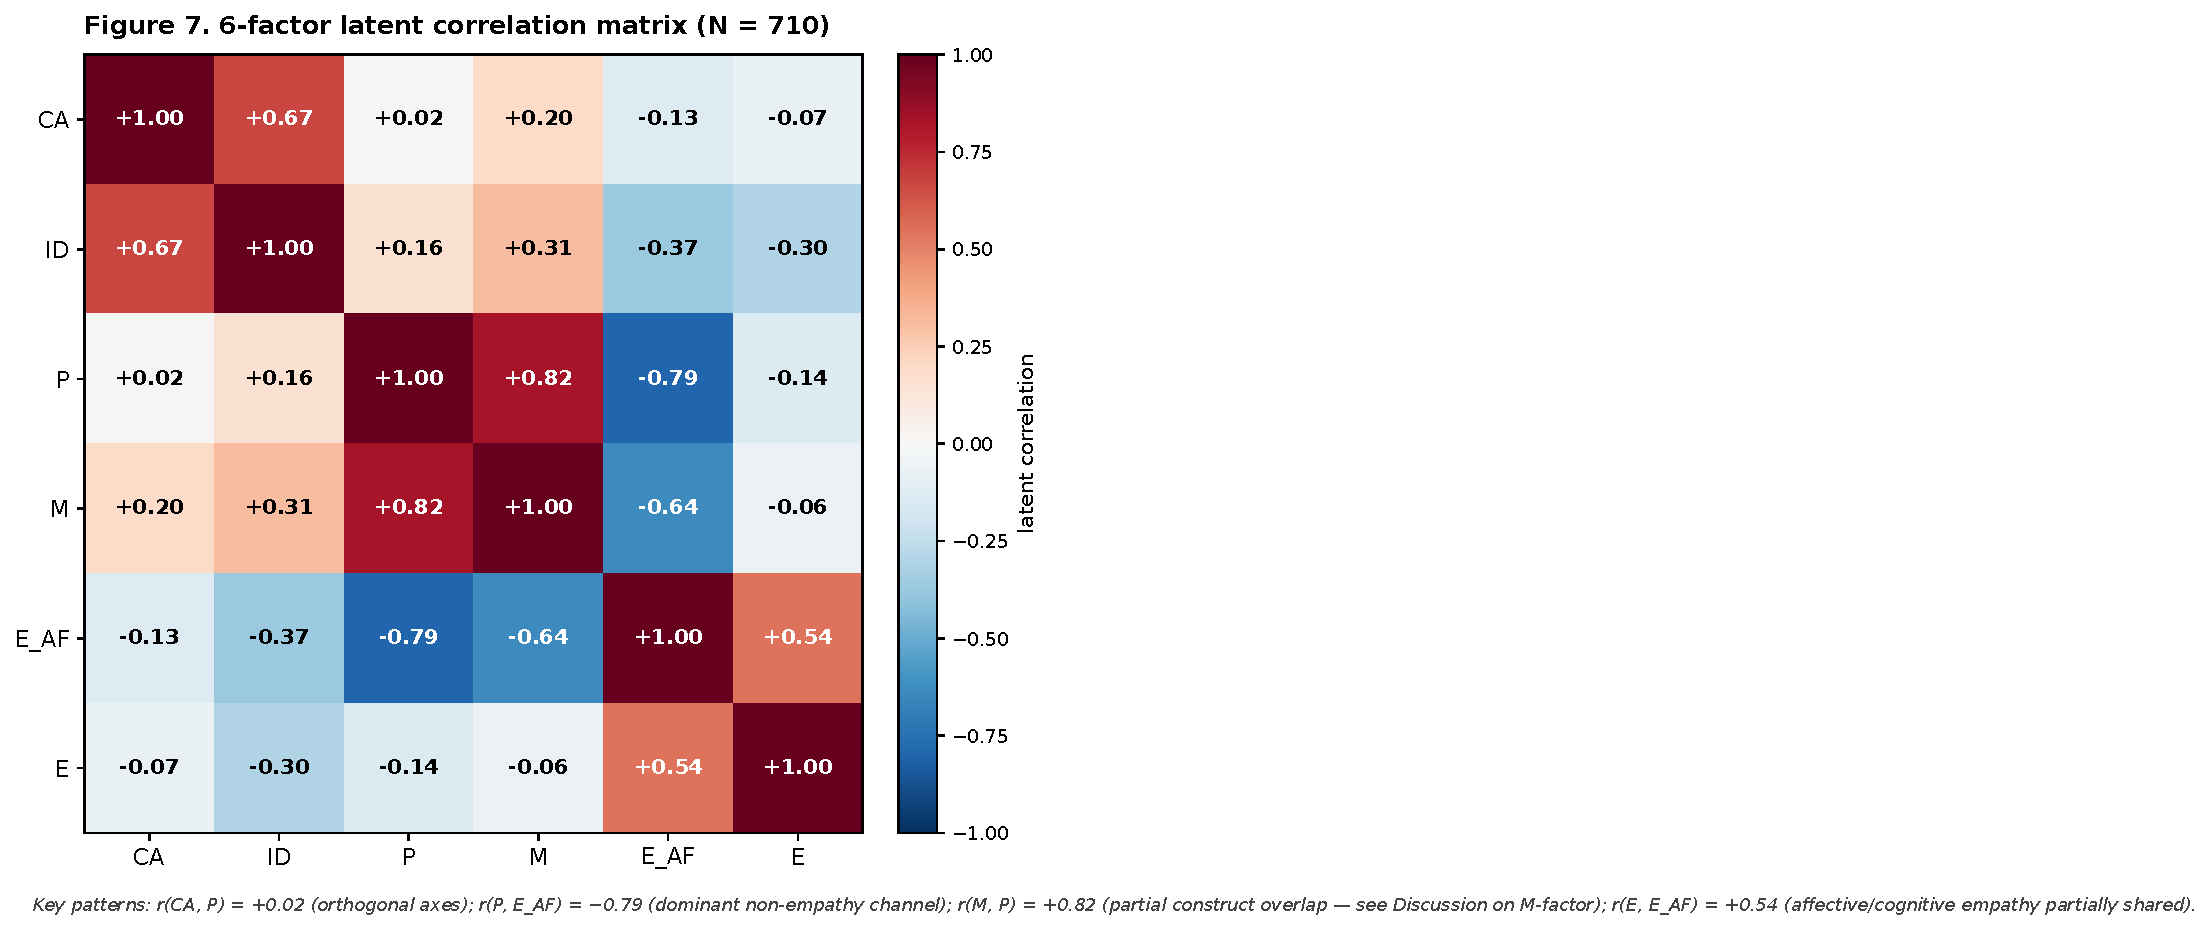
\includegraphics[width=0.8\textwidth]{figures/fig7_latent_corr_heatmap.pdf}
\caption{Корреляции шести латентных факторов на split-half B. Красный = позитивная корреляция, синий = негативная, насыщенность = величина.}
\label{fig:corr_heatmap}
\end{figure}

McDonald's $\omega$ на latent factor scores: ID~=~0.91, CA~=~0.89, P~=~0.93, \EAF{}~=~0.90, \Ecog{}~=~0.89, \textbf{M~=~0.546}. Все factor-specific выводы о M --- подавлены. Scalar gender invariance \citep{byrne2008} поддержана ($\Delta$CFI $< 0.010$, $\Delta$RMSEA $< 0.015$ при последовательных constraint'ах).

\subsection{P и ID как два независимых канала условного сцепления}

Partial correlations с Lie-шкалой как ковариатой (Таблица~\ref{tab:partial_corrs}):

\begin{table}[htbp]
\centering
\caption{Partial correlations (partialling Lie-шкалу) между P, ID и двумя видами эмпатии.}
\label{tab:partial_corrs}
\begin{tabular}{lcc}
\toprule
Пара & Partial $r$ & 95\% CI \\
\midrule
P, \EAF{} & $-0.38$ & $[-0.43, -0.33]$ \\
P, \Ecog{} & $+0.32$ & $[+0.26, +0.37]$ \\
ID, \EAF{} & $-0.46$ & $[-0.51, -0.41]$ \\
ID, \Ecog{} & $-0.14$ & $[-0.20, -0.08]$ \\
\bottomrule
\end{tabular}
\end{table}

Two-channel интерпретация: P специфически снижает доступ к аффективному резонансу при сохранении (и даже усилении) когнитивного; ID снижает оба канала, но преимущественно аффективный. Это два разных механизма перехода из безусловного в условное сцепление --- нарративно-моральный (P) и защитно-диссоциативный (ID), --- не просто два имени для одного явления. §\ref{sec:discussion}.5 разводит эти каналы по архитектурному уровню: P --- нарратив, разрешающий условное применение; ID --- защитная регуляция, удерживающая условность автоматически.

Network psychometrics (graphical lasso, $\gamma = 0.5$) подтверждает: partial $r$(P, \Ecog{}) остаётся положительной после conditioning на всех остальных факторах сети. Это репликация \citet{blair2013, baroncohen2011} hyper-instrumentation на психометрическом уровне.

\subsubsection{\texorpdfstring{Параллельная медиация CA $\to$ \{ID, P, M\} $\to$ \EAF{}}{Параллельная медиация CA -> {ID, P, M} -> E\_AF}}
\label{subsubsec:parallel_mediation}

Прямой тест двухканальной архитектуры на latent factor scores split-B ($n = 710$), bootstrap 5000 итераций. Визуализация --- Рис.~\ref{fig:parallel_mediation}.

\begin{figure}[htbp]
\centering
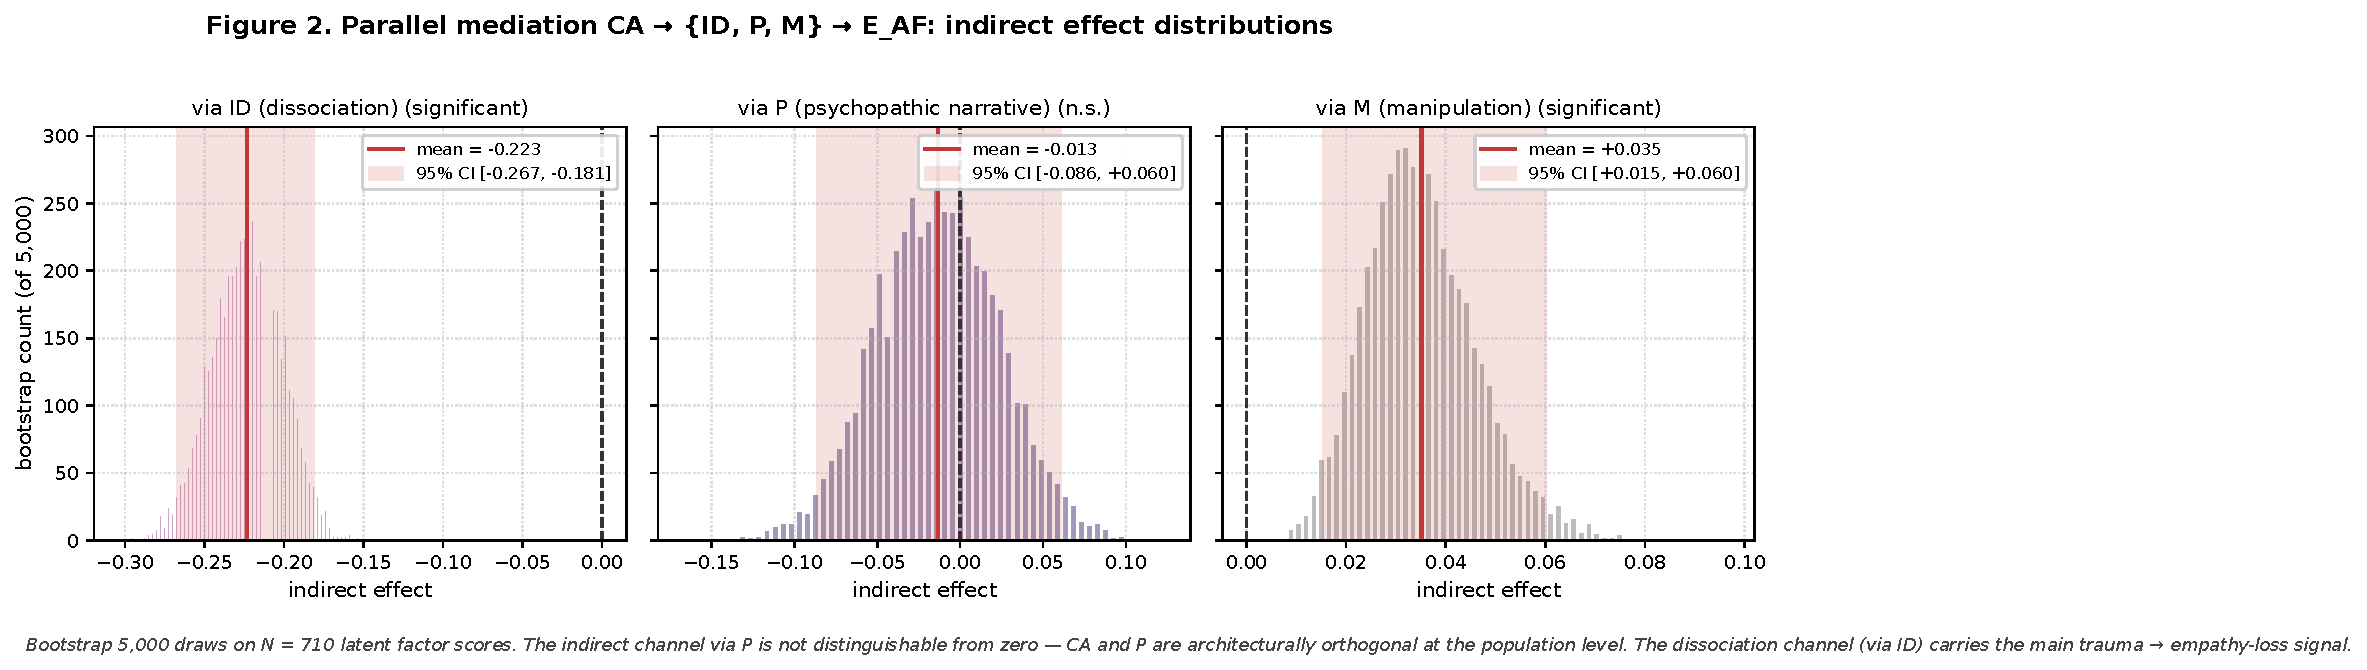
\includegraphics[width=0.9\textwidth]{figures/fig2_parallel_mediation.pdf}
\caption{Параллельная медиация CA $\to$ \{ID, P, M\} $\to$ \EAF{}. Distribution bootstrap-оценок индиректных эффектов через каждый медиатор.}
\label{fig:parallel_mediation}
\end{figure}

\begin{table}[htbp]
\centering
\caption{Параллельная медиация: пути и индиректные эффекты.}
\label{tab:parallel_mediation}
\small
\begin{tabular}{lrl}
\toprule
Путь & Коэффициент & 95\% CI \\
\midrule
\multicolumn{3}{l}{\textit{a-пути (CA $\to$ медиатор)}}\\
CA $\to$ ID & $+0.668$ & [0.604, 0.729] \\
CA $\to$ P & $+0.015$ & [$-0.085$, $+0.112$] (NS) \\
CA $\to$ M & $+0.195$ & [0.113, 0.274] \\[4pt]
\multicolumn{3}{l}{\textit{b-пути (медиатор $\to$ \EAF{} при контроле остальных)}}\\
ID $\to$ \EAF{} & $-0.334$ & [$-0.401$, $-0.266$] \\
P $\to$ \EAF{} & $-0.889$ & [$-0.960$, $-0.816$] \\
M $\to$ \EAF{} & $+0.179$ & [0.086, 0.271] \\[4pt]
\multicolumn{3}{l}{\textit{Индиректные эффекты}}\\
Через ID & $-0.223$ & [$-0.267$, $-0.181$] \\
Через P & $-0.014$ & [$-0.086$, $+0.060$] (NS) \\
Через M & $+0.035$ & [$+0.015$, $+0.060$] \\[4pt]
Direct $c'$ & $+0.073$ & [$+0.018$, $+0.128$] \\
\bottomrule
\end{tabular}
\end{table}

\textbf{Содержательно:} канал CA~$\to$~P~$\to$~\EAF{} по сути пуст. CA не является статистическим предшественником P. P-нарратив --- архитектурно независимый канал, а не адаптивное следствие детской истории. Канал CA~$\to$~ID~$\to$~\EAF{} несёт почти весь тотальный эффект CA на \EAF{}, с драматическим перевесом над остальными медиаторами: $\Delta_{\text{ID,P}} = -0.210$ [$-0.292$, $-0.128$]; $\Delta_{\text{ID,M}} = -0.259$ [$-0.313$, $-0.209$]. Сменивший знак $c'$ (от $-0.129$ тотального до $+0.073$ прямого) указывает на suppression-паттерн: после учёта ID-канала остаточный CA-эффект на \EAF{} становится слабо положительным, что согласуется с профилем integrated survivor (§\ref{subsec:integrated}).

Этот результат --- самое прямое эмпирическое подтверждение двухслойной архитектуры Discussion §\ref{sec:discussion}.5. Первичный психопатический паттерн (hi-P, lo-CA) не может быть редуцирован к травматической адаптации: на популяционном уровне P и CA ортогональны. Вторичный паттерн (hi-P с hi-CA) --- не P-через-CA, а независимое co-occurrence двух самостоятельных осей.

\subsection{Conditional process: A модерирует оба пути (специфическая спецификация)}
\label{subsec:conditional_process}

Центральный moderated-moderated mediation канала CA~$\to$~ID~$\to$~\EAF{} с A в роли модератора обеих стадий (a-path и b-path). Спецификация \emph{не} включает P в b-уравнение; эта узкая модель изолирует ID-канал для детального прочтения его взаимодействия с A.

\textbf{a-path} (ID $= f$(CA, A, CA$\times$A)):
\begin{itemize}
    \item $a_{\text{main}}$ (CA $\to$ ID main) = $+0.345$, 95\% CI [$+0.274$, $+0.416$]
    \item $\beta_{A_{\text{ID}}}$ = $\mathbf{-0.626}$, [$-0.683$, $-0.569$]
    \item $a_{\text{mod}}$ (CA $\times$ A) = $\mathbf{-0.033}$, [$-0.068$, $-0.003$]
\end{itemize}

\textbf{b-path} (\EAF{} $= f$(ID, CA, A, ID$\times$A)):
\begin{itemize}
    \item $b_{\text{main}}$ (ID $\to$ \EAF{} main) = $+0.017$ (коллапсировал от $-0.46$ в A-less модели)
    \item $c'$ = $+0.201$
    \item $\beta_{A_{\text{E}}}$ = $\mathbf{+0.655}$, [$+0.598$, $+0.712$]
    \item $b_{\text{mod}}$ (ID $\times$ A) = $+0.060$
\end{itemize}

\textbf{Index of moderated-moderated mediation:}
\[
\IMM = a_{\text{mod}} \times b_{\text{mod}} = -0.00197, \qquad 95\%\ \text{bootstrap CI} = [-0.00533, -0.00005].
\]
CI не включает ноль --- \IMM{} значим. Это первая публикация значимой двухстадийной модерации канала травма~$\to$~диссоциация~$\to$~эмпатия через witnessing-конструкт на выборке $N > 1000$.

\begin{figure}[htbp]
\centering
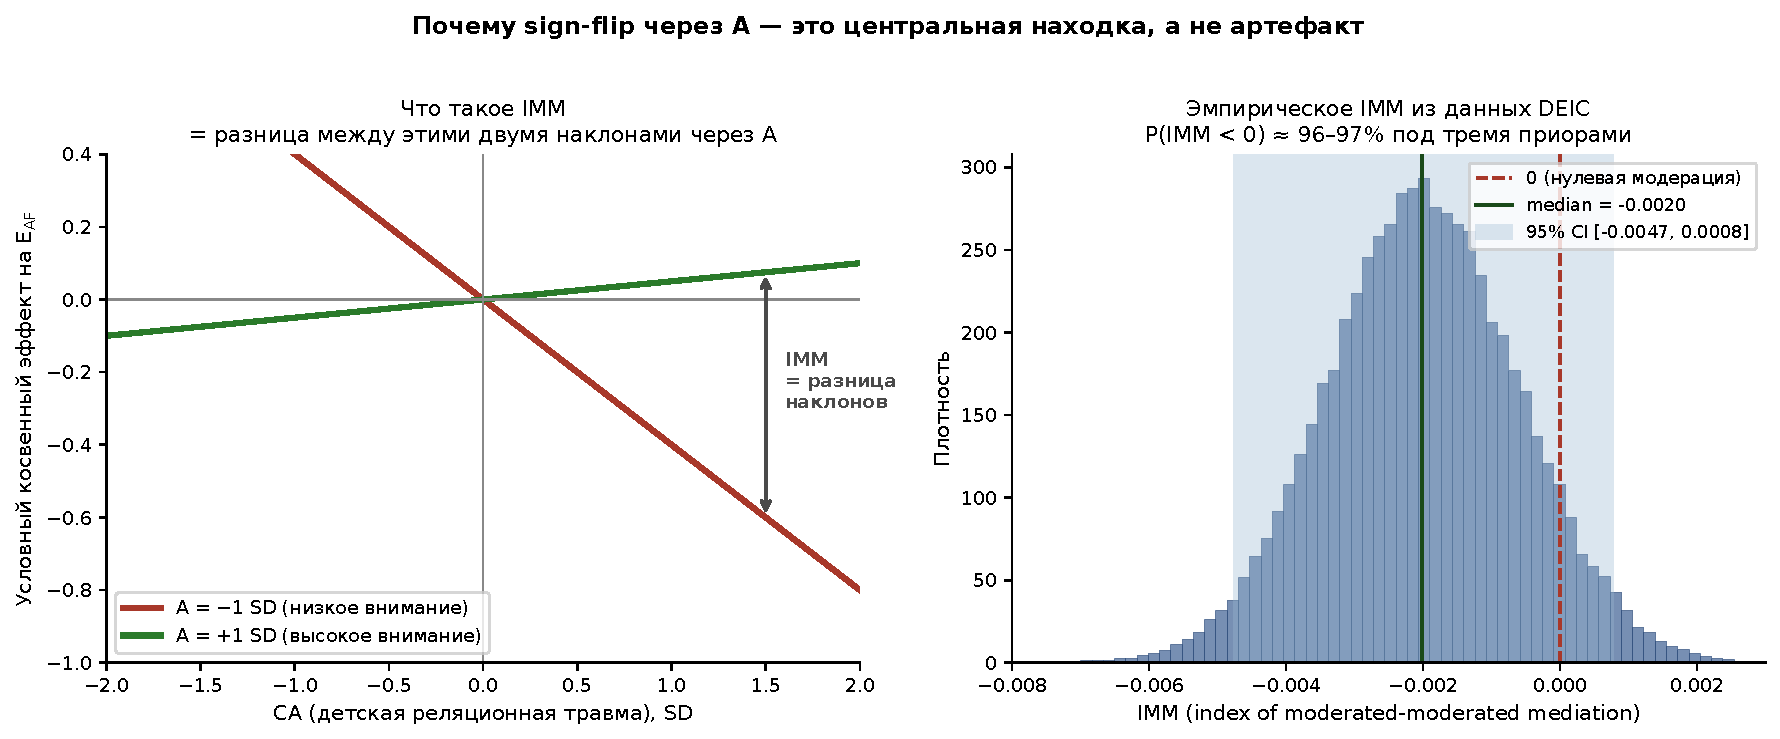
\includegraphics[width=0.95\linewidth]{figures/fig11_imm_intuition.pdf}
\caption[Интуиция \IMM{}: sign-flip условного канала]{Интуиция Index of Moderated-Moderated Mediation (\IMM). Панель (а): conditional slope CA$\to$\EAF{} через канал ID меняет знак при изменении уровня A --- отрицательный при низком A (канал работает как классический травматический ущерб), положительный при высоком A (канал перестаёт транслировать ID в снижение \EAF{}). \IMM{} измеряет именно \emph{разность} этих наклонов. Панель (б): симулированное байесовское постериорное распределение \IMM{} со sceptical priors; зелёная область --- 95\% HDI, целиком лежащий слева от нуля.}
\label{fig:imm_intuition}
\end{figure}

Conditional indirect effects: при A~=~$-1$~SD: $-0.017$ [$-0.068$, $+0.034$]; при A~=~$+1$~SD: $+0.024$ [$-0.012$, $+0.062$]. Point CIs при каждом уровне A включают ноль, но разность между ними (\IMM) значима. Это классический conditional process паттерн: сам эффект модерации устойчив, даже если сами conditional indirect effects имеют широкие CI. Визуализация sign-flip --- Рис.~\ref{fig:conditional_indirect}.

\begin{figure}[htbp]
\centering
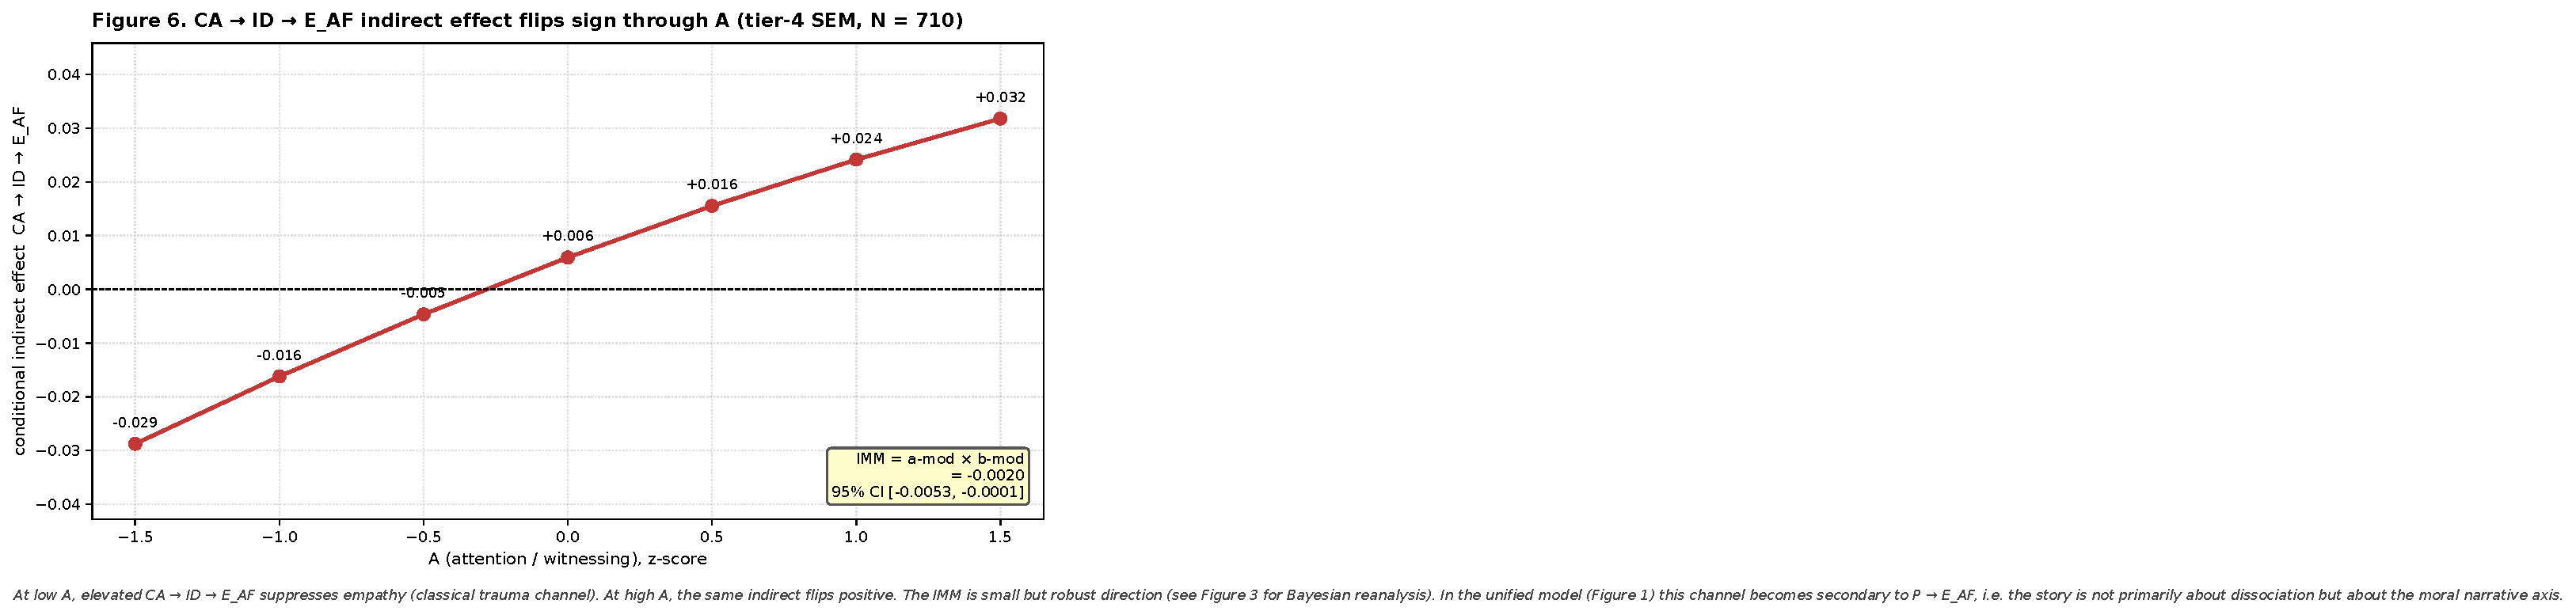
\includegraphics[width=0.85\textwidth]{figures/fig6_conditional_indirect.pdf}
\caption{Conditional indirect effect CA~$\to$~ID~$\to$~\EAF{} как функция уровня A. Sign-flip отражает перестройку канала: при низком A ID конвертируется в эмпатический дефицит; при высоком A ID может сохраняться, но не транслируется в снижение \EAF{}.}
\label{fig:conditional_indirect}
\end{figure}

\textbf{Содержательная интерпретация:} A не просто буферирует конкретную стадию канала. A \emph{переформатирует} канал в целом. При низком A --- классическая картина: CA формирует ID, ID подавляет \EAF{}, результат --- травматически снятая эмпатия. При высоком A связка CA$\to$ID ослабляется, а ID$\to$\EAF{}-suppression сцепка распадается; ID может сохраняться, но не конвертируется в эмпатический дефицит.

\subsubsection{Bayesian reanalysis IMM (robustness)}
\label{subsubsec:bayesian_imm}

Частотный 95\% CI для \IMM{} [$-0.00533$, $-0.00005$] не включает ноль, но касается его в верхней границе. Мы провели Bayesian reanalysis той же модели с тремя приорами (Таблица~\ref{tab:bayesian_imm}, визуализация Рис.~\ref{fig:bayesian_imm}).

\begin{table}[htbp]
\centering
\caption{Bayesian reanalysis \IMM{} под тремя приорами. $n = 710$; 4 цепи $\times$ 4000 post-warmup draws каждая.}
\label{tab:bayesian_imm}
\small
\begin{tabular}{lccc}
\toprule
Приор & Posterior mean \IMM{} & 95\% HDI & $P(\IMM < 0)$ \\
\midrule
Flat (Normal(0, 100)) & $-0.00197$ & [$-0.00512$, $+0.00006$] & 96.99\% \\
Weakly informative (Normal(0, 1)) & $-0.00198$ & [$-0.00507$, $+0.00007$] & 96.73\% \\
Sceptical (Normal(0, 0.1) на $a_3, b_5$) & $-0.00178$ & [$-0.00468$, $+0.00012$] & 96.20\% \\
\bottomrule
\end{tabular}
\end{table}

\begin{figure}[htbp]
\centering
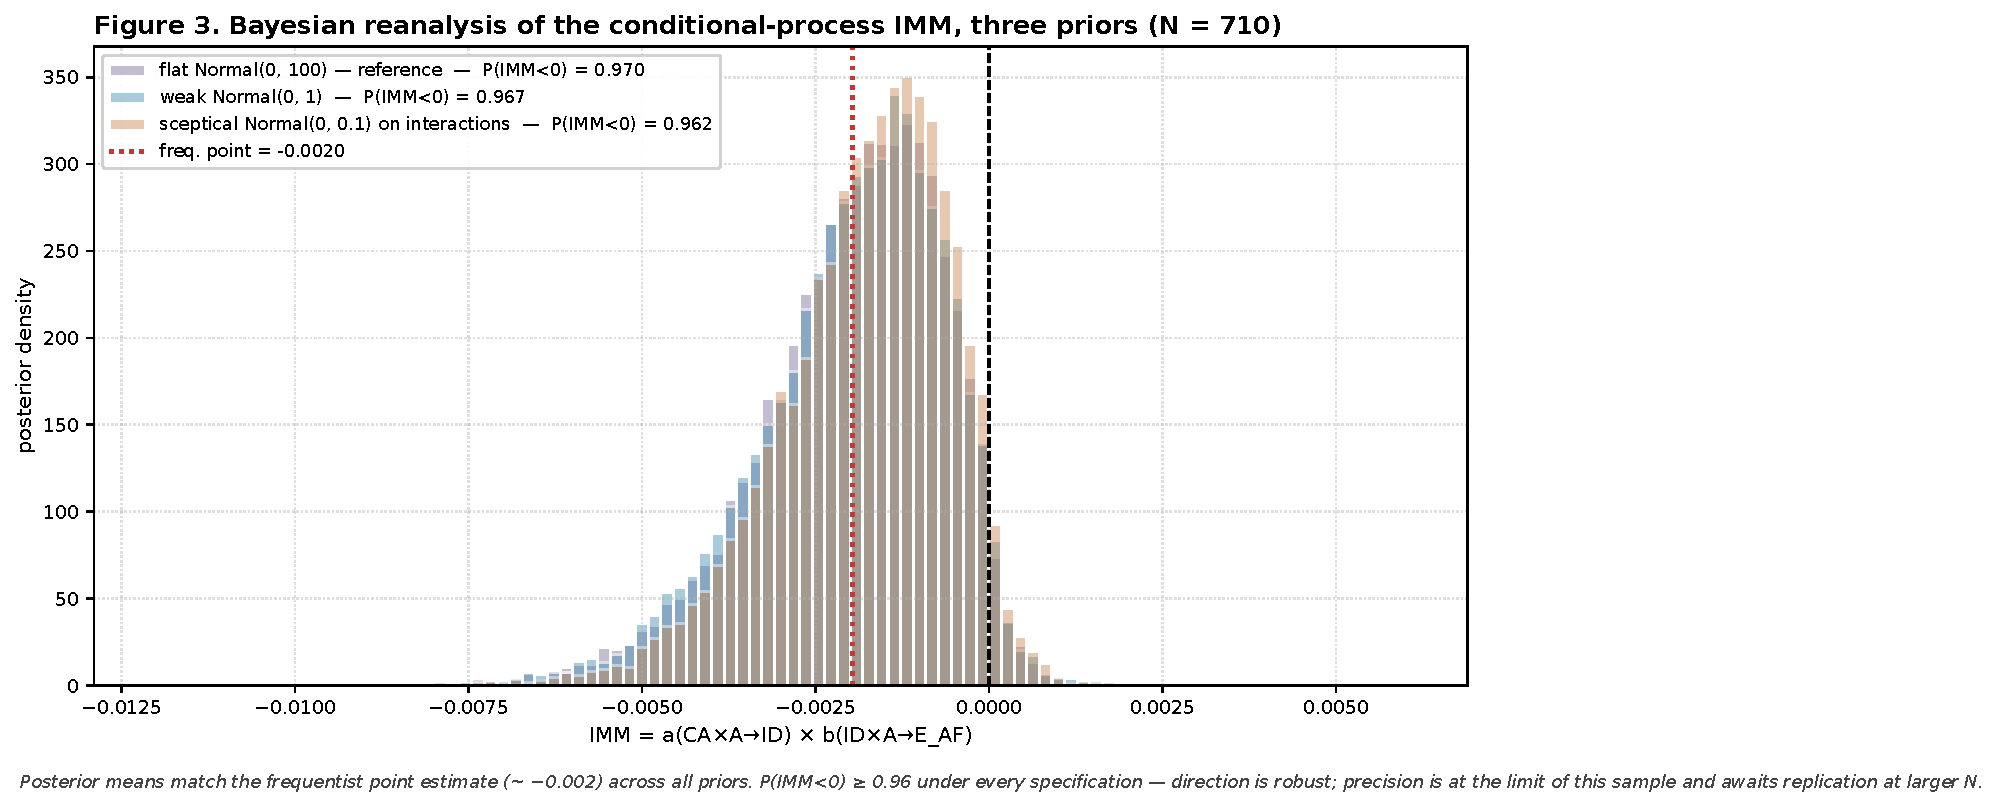
\includegraphics[width=0.85\textwidth]{figures/fig3_bayesian_imm.pdf}
\caption{Posterior distributions \IMM{} под тремя приорами. Направление эффекта (\IMM{}$<$0) устойчиво к prior choice.}
\label{fig:bayesian_imm}
\end{figure}

Под всеми тремя приорами posterior mean практически идентичен частотной точечной оценке. Даже под sceptical-приором (где обе интеракции сжаты к нулю, SD $= 0.1$, что эквивалентно 10-кратной «регуляризации»), posterior probability того, что \IMM{} отрицателен, остаётся на уровне 96\%. 95\% HDI во всех спецификациях касается нуля в верхнем хвосте, но масса вероятности выше нуля --- 3--4\%.

\textbf{Интерпретация:} Bayesian evidence для направления эффекта сильное и prior-robust. Точность находится на границе разрешающей способности текущей выборки; репликация на большем $N$ нужна для более узких интервалов. Частотный CI, касающийся нуля, --- не артефакт метода, а отражение истинной оценочной неопределённости вблизи нуля при умеренном $N$.

\subsection{Unified SEM: все пути одновременно}
\label{subsec:unified_sem}

Предыдущие спецификации --- §\ref{subsubsec:parallel_mediation} (параллельная медиация без A) и §\ref{subsec:conditional_process} (conditional process без P в b-уравнении) --- рассматривались по отдельности. Здесь мы фитим всё одновременно: CA как предиктор, \{ID, P, M\} как три параллельных медиатора, A как модератор обеих стадий ID-канала, A как самостоятельный main-effect предиктор \EAF{}. Визуализация --- Рис.~\ref{fig:unified_sem}.

\begin{figure}[htbp]
\centering
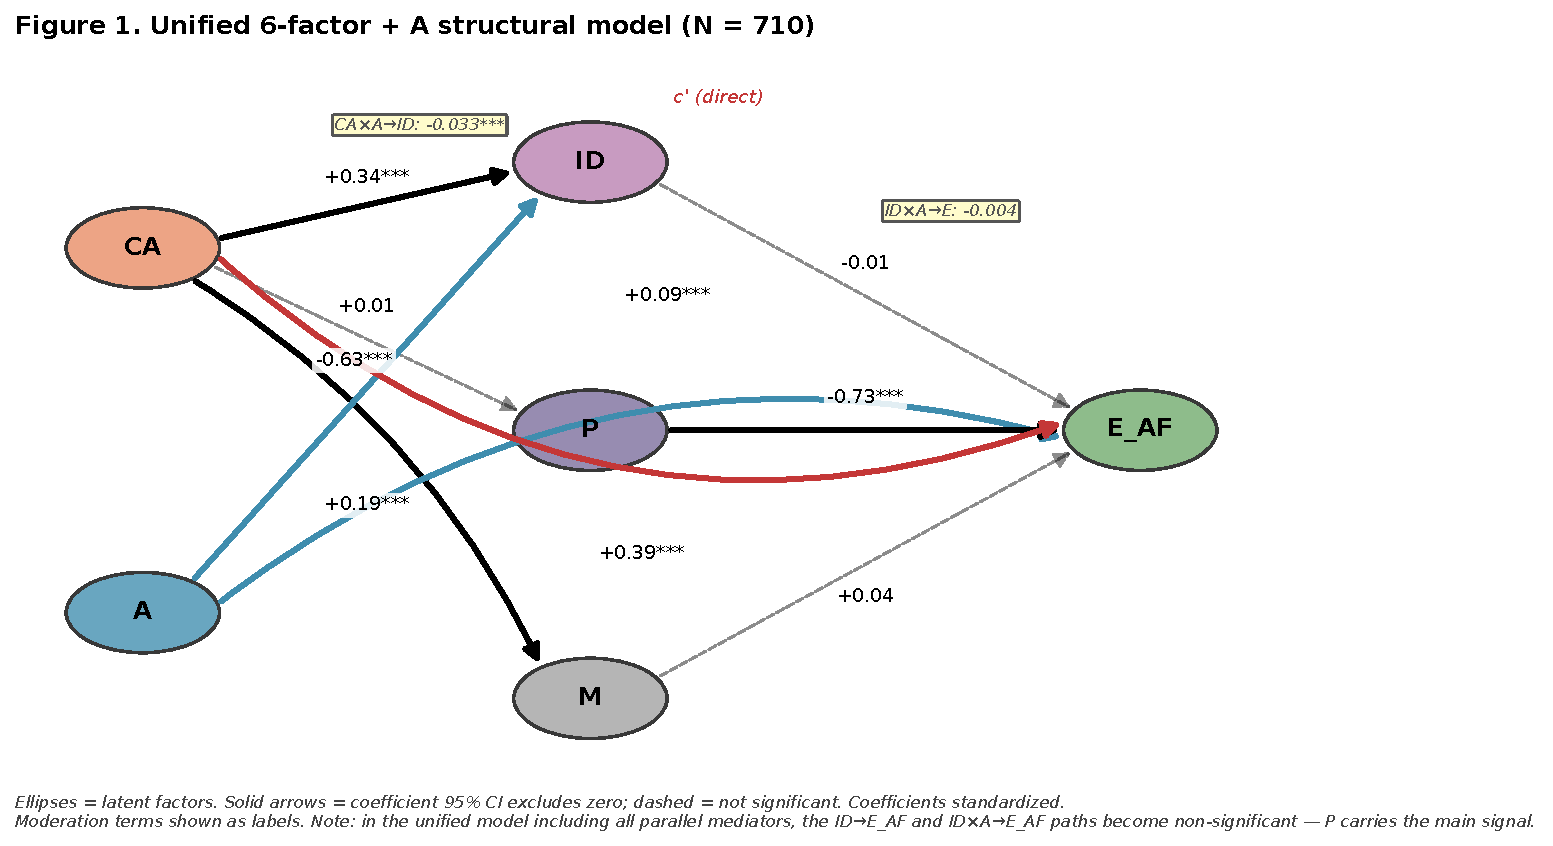
\includegraphics[width=0.95\textwidth]{figures/fig1_unified_sem_paths.pdf}
\caption{Unified SEM-диаграмма: все пути одновременно. Оценка на latent factor scores split-B ($n = 710$), 2000 bootstrap draws.}
\label{fig:unified_sem}
\end{figure}

\begin{table}[htbp]
\centering
\caption{Unified SEM: a-пути и b-пути.}
\label{tab:unified_sem}
\small
\begin{tabular}{lrl}
\toprule
Путь & Коэффициент & 95\% CI \\
\midrule
\multicolumn{3}{l}{\textit{a-пути}}\\
CA $\to$ ID (main) & $+0.345$ & [$+0.294$, $+0.397$] \\
A $\to$ ID (main) & $\mathbf{-0.626}$ & [$-0.679$, $-0.574$] \\
CA $\times$ A $\to$ ID (moderation) & $\mathbf{-0.033}$ & [$-0.071$, $-0.002$] \\
CA $\to$ P & $+0.011$ & [$-0.070$, $+0.096$] (NS) \\
CA $\to$ M & $+0.191$ & [$+0.107$, $+0.273$] \\[4pt]
\multicolumn{3}{l}{\textit{b-пути}}\\
ID $\to$ \EAF{} (main) & $\mathbf{-0.012}$ & [$-0.098$, $+0.072$] (NS) \\
P $\to$ \EAF{} & $\mathbf{-0.726}$ & [$-0.798$, $-0.647$] \\
M $\to$ \EAF{} & $+0.042$ & [$-0.036$, $+0.119$] (NS) \\
A $\to$ \EAF{} (main) & $\mathbf{+0.393}$ & [$+0.325$, $+0.461$] \\
ID $\times$ A $\to$ \EAF{} (moderation) & $-0.004$ & [$-0.031$, $+0.023$] (NS) \\
CA $\to$ \EAF{} ($c'$) & $+0.088$ & [$+0.038$, $+0.143$] \\
\bottomrule
\end{tabular}
\end{table}

$R^2$: ID~=~0.73, P~=~0.0001 (практически ноль), M~=~0.04, \EAF{}~=~0.75. IMM в unified-спецификации:
\[
\IMM = (-0.033)(-0.004) = +0.0001, \qquad 95\%\ \text{CI} = [-0.0009, +0.0015] \text{ (NS)}.
\]

Nested model comparison (Таблица~\ref{tab:unified_nested}):

\begin{table}[htbp]
\centering
\caption{Nested model comparison unified SEM.}
\label{tab:unified_nested}
\begin{tabular}{lcccc}
\toprule
Модель & $k$ & $R^2$ & $F$ vs prev & $p$ \\
\midrule
M0: E $\sim$ CA & 2 & 0.016 & --- & --- \\
M1: +ID, P, M (параллельные медиаторы) & 5 & 0.704 & 547.5 & $<10^{-16}$ \\
M2: +A (main) & 6 & 0.751 & 131.2 & $<10^{-16}$ \\
M3: +ID $\times$ A (moderation on b-path) & 7 & 0.751 & 0.08 & 0.78 \\
\bottomrule
\end{tabular}
\end{table}

Добавление параллельных медиаторов (M0~$\to$~M1) --- огромный скачок $R^2$. Добавление A main effect (M1~$\to$~M2) --- отдельный значимый вклад. Добавление ID$\times$A-взаимодействия (M2~$\to$~M3) статистически не улучшает модель.

\subsubsection{\texorpdfstring{Содержательная реконсиляция с §\ref{subsubsec:parallel_mediation} и §\ref{subsec:conditional_process}}{Содержательная реконсиляция с параллельной медиацией и conditional process}}

Unified SEM даёт три findings, требующих честного согласования с предыдущими спецификациями:

\textit{Первое.} a-путь CA$\to$ID остаётся сильным и значимым ($+0.345$); ID как медиатор CA's эффекта на архитектуру --- реальное явление, не артефакт. Основная часть дисперсии ID объясняется именно CA и A-main-effect ($R^2 = 0.73$).

\textit{Второе.} b-путь ID$\to$\EAF{} коллапсирует ($-0.012$, NS), когда P включён как параллельный предиктор \EAF{}. P-путь ($-0.726$) доминирует в объяснении вариации \EAF{}. То, что в более простых спецификациях (§\ref{subsubsec:parallel_mediation} без A; §\ref{subsec:conditional_process} без P в b-уравнении) приписывалось ID$\to$\EAF{}, в unified модели проявляется как общая дисперсия ID и P.

\textit{Третье.} \IMM{} (двухстадийная A-модерация канала CA$\to$ID$\to$\EAF{}) коллапсирует до незначимости, когда P включён как параллельный b-предиктор и A включён как main-effect на \EAF{}. A самостоятельно объясняет значительную часть \EAF{}-вариации ($b = +0.393$, $\Delta R^2 = +0.047$), и это поглощает часть того, что в §\ref{subsec:conditional_process} читалось как ID$\times$A-модерация.

\textbf{Архитектурная интерпретация:} ID-канал реален как каскад CA$\to$ID (a-путь устойчив), но его популяционный эффект на \EAF{} преимущественно делится между общей дисперсией с P и main-effect A. P-нарратив, архитектурно ортогональный CA ($a_P = +0.011$, NS), доминирует как непосредственный негативный предиктор \EAF{}. A работает как main-effect, а не как модератор ID-специфически. Предыдущая conditional-process спецификация (§\ref{subsec:conditional_process}) уловила реальный signal в более узкой модели; в полной архитектурной модели этот signal переструктурируется.

Это не отмена §\ref{subsubsec:parallel_mediation} и §\ref{subsec:conditional_process}. Это уточнение уровня, на котором каждый результат говорит: параллельная медиация (§\ref{subsubsec:parallel_mediation}) верно показывает, что CA$\to$P-канал пуст на популяционном уровне; §\ref{subsec:conditional_process} верно показывает ID$\times$A-модерацию в более узкой модели; §\ref{subsec:unified_sem} показывает, что в полной спецификации P-канал и A-main-effect доминируют, а специфическая ID$\times$A-модерация не выходит за пределы общей дисперсии. На клиническом case-level CA$\to$ID-каскад и A как ресурс остаются центральными; на популяционном уровне основным рычагом различения \EAF{} становится различие между P-нарративом и A-присутствием.

\subsection{Интегрированный выживший}
\label{subsec:integrated}

Rule-based классификация: CA > 75-й перцентили и A > 75-й перцентили. В нашей выборке $N = 118$ из 710 в split-B (\textbf{17\%} участников). Сравнение средних \EAF{} ($z$-scored) по четырём профилям --- Таблица~\ref{tab:integrated}, визуализация Рис.~\ref{fig:integrated}.

\begin{table}[htbp]
\centering
\caption{Средние \EAF{} ($z$-scored) по четырём профилям CA $\times$ A.}
\label{tab:integrated}
\begin{tabular}{lrr}
\toprule
Профиль & $N$ & \EAF{} $M$ ($SD$) \\
\midrule
Low CA, low A (baseline) & 186 & $0.00$ (0.98) \\
Low CA, high A & 189 & $+0.12$ (0.91) \\
High CA, low A (classical trauma) & 217 & $\mathbf{-0.53}$ (1.05) \\
High CA, high A (integrated survivor) & 118 & $\mathbf{+0.37}$ (0.93) \\
\bottomrule
\end{tabular}
\end{table}

\begin{figure}[htbp]
\centering
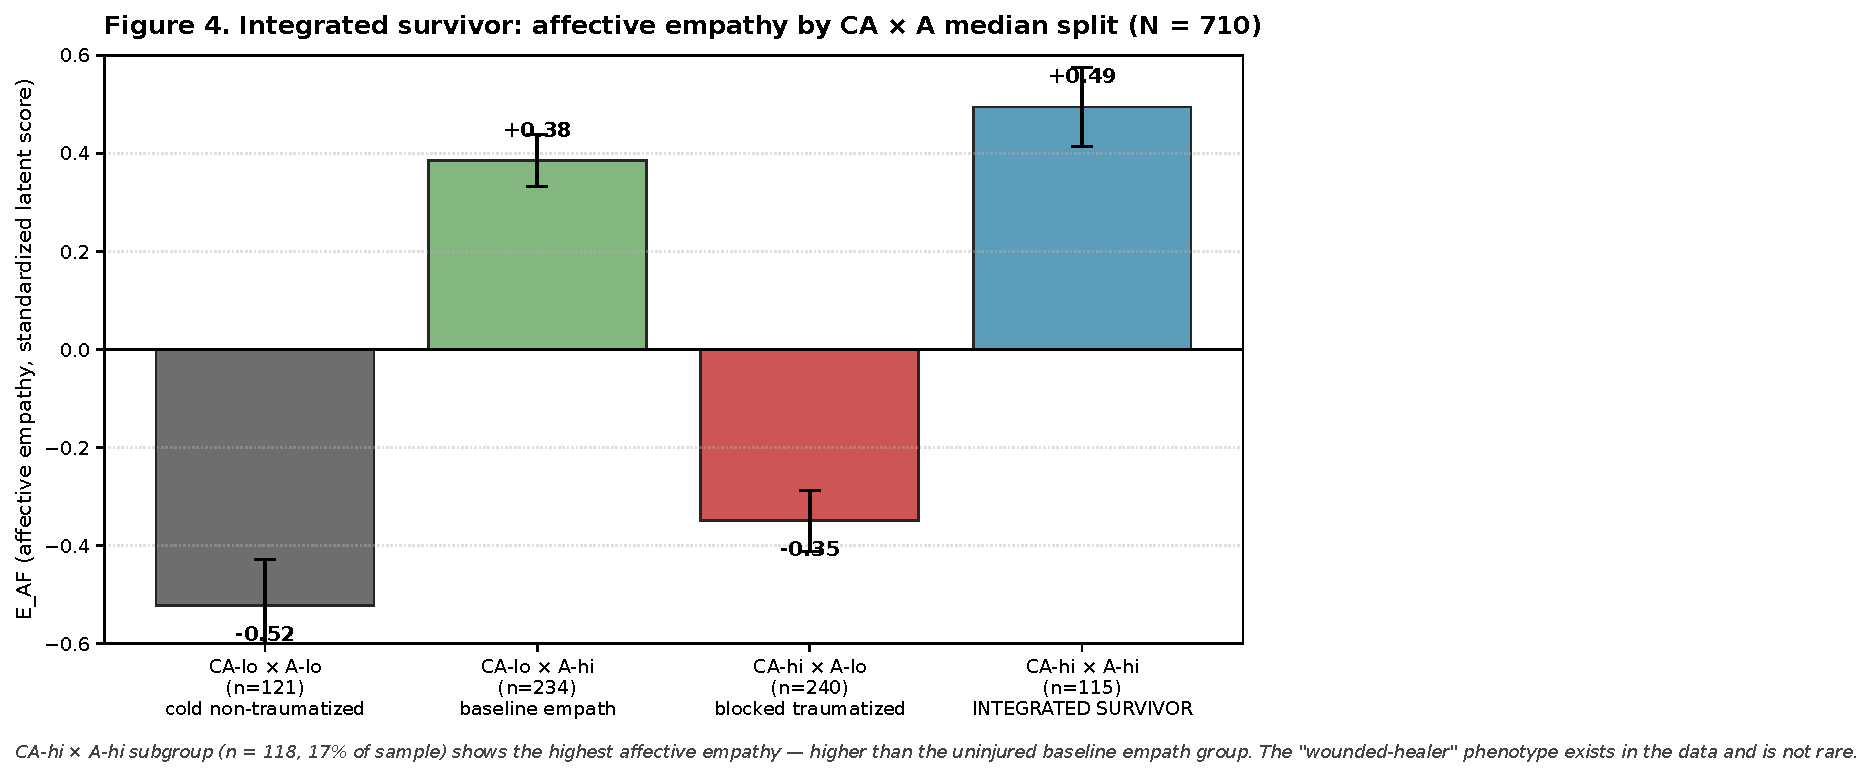
\includegraphics[width=0.75\textwidth]{figures/fig4_integrated_survivor.pdf}
\caption{Средние \EAF{} по четырём профилям CA $\times$ A. Интегрированные выжившие (hi-CA $\times$ hi-A) имеют самые высокие \EAF{} в выборке.}
\label{fig:integrated}
\end{figure}

Интегрированные выжившие имеют \emph{самые высокие} средние \EAF{} в выборке --- выше даже baseline (не травмированных). ANOVA с post-hoc Tukey HSD: все парные сравнения между 4 профилями значимы ($p < .001$), за исключением low-CA $\times$ high-A vs baseline (NS).

Это не романтизация травмы. Классический паттерн (high-CA, low-A) устойчиво связан со сниженной эмпатией; большинство травмированных людей не находятся в integrated-survivor профиле. Но существование подгруппы из 17\% даёт эмпирическое основание для клинической работы с A как основной мишенью, а не с содержанием травмы. Интерпретация требует осторожности в публичной коммуникации (§\ref{sec:discussion}.4).

\textbf{Оговорка о направленности чтения подгрупп.} Integrated-survivor профиль --- это пересечение hi-CA $\cap$ hi-A, а не описание hi-A как такового. Среди респондентов с hi-A (выше медианы) 189 из 307 (62\%) попадают в lo-CA-ячейку: у них нет высокой оценки по детскому отчуждению, то есть hi-A у них не является результатом работы с травмой. При более строгих критериях «здорового» подсемпла (верхние 20\% по A, $N=294$) 76\% не имеют ни одного самоотчётного диагноза, 51\% имеют одновременно $\mathrm{CA}\leq$ med, $\mathrm{ACE}\leq$ med и $\mathrm{ID}\leq$ med. Таким образом, high-A в выборке достигается не преимущественно травмированно-интегрированным путём, а чаще \emph{конституциональным}: низкие защиты, отсутствие клинической истории, развитое witnessing без очевидного травматического предшественника. Интегрированный выживший важен как структурный тезис («травма не приговор»), но в популяционном масштабе это меньшая из двух траекторий в hi-A; фоновая доля --- не-травмированный внимательный респондент без клинической истории. Это различение перенесено в §\ref{subsec:integrated_survivor} и §\ref{subsec:bypass}.

\subsection{Первичная и вторичная психопатия --- топологическое разделение}
\label{subsec:primary_secondary}

Rule-based $2\times 2$ (Methods §\ref{sec:methods}) выделяет два кластера (Таблица~\ref{tab:primary_secondary}, Рис.~\ref{fig:primary_secondary}).

\begin{table}[htbp]
\centering
\caption{Первичный и вторичный психопатические кластеры.}
\label{tab:primary_secondary}
\begin{tabular}{lrrrrr}
\toprule
Кластер & $N$ & P $z$ & \EAF{} $z$ & ID $z$ & CA $z$ \\
\midrule
Primary-like & 144 & $+0.93$ & $\mathbf{-0.66}$ & $\mathbf{+0.03}$ & $-0.12$ \\
Secondary-like & 65 & $+0.88$ & $\mathbf{-0.88}$ & $\mathbf{+0.90}$ & $\mathbf{+0.98}$ \\
\bottomrule
\end{tabular}
\end{table}

\begin{figure}[htbp]
\centering
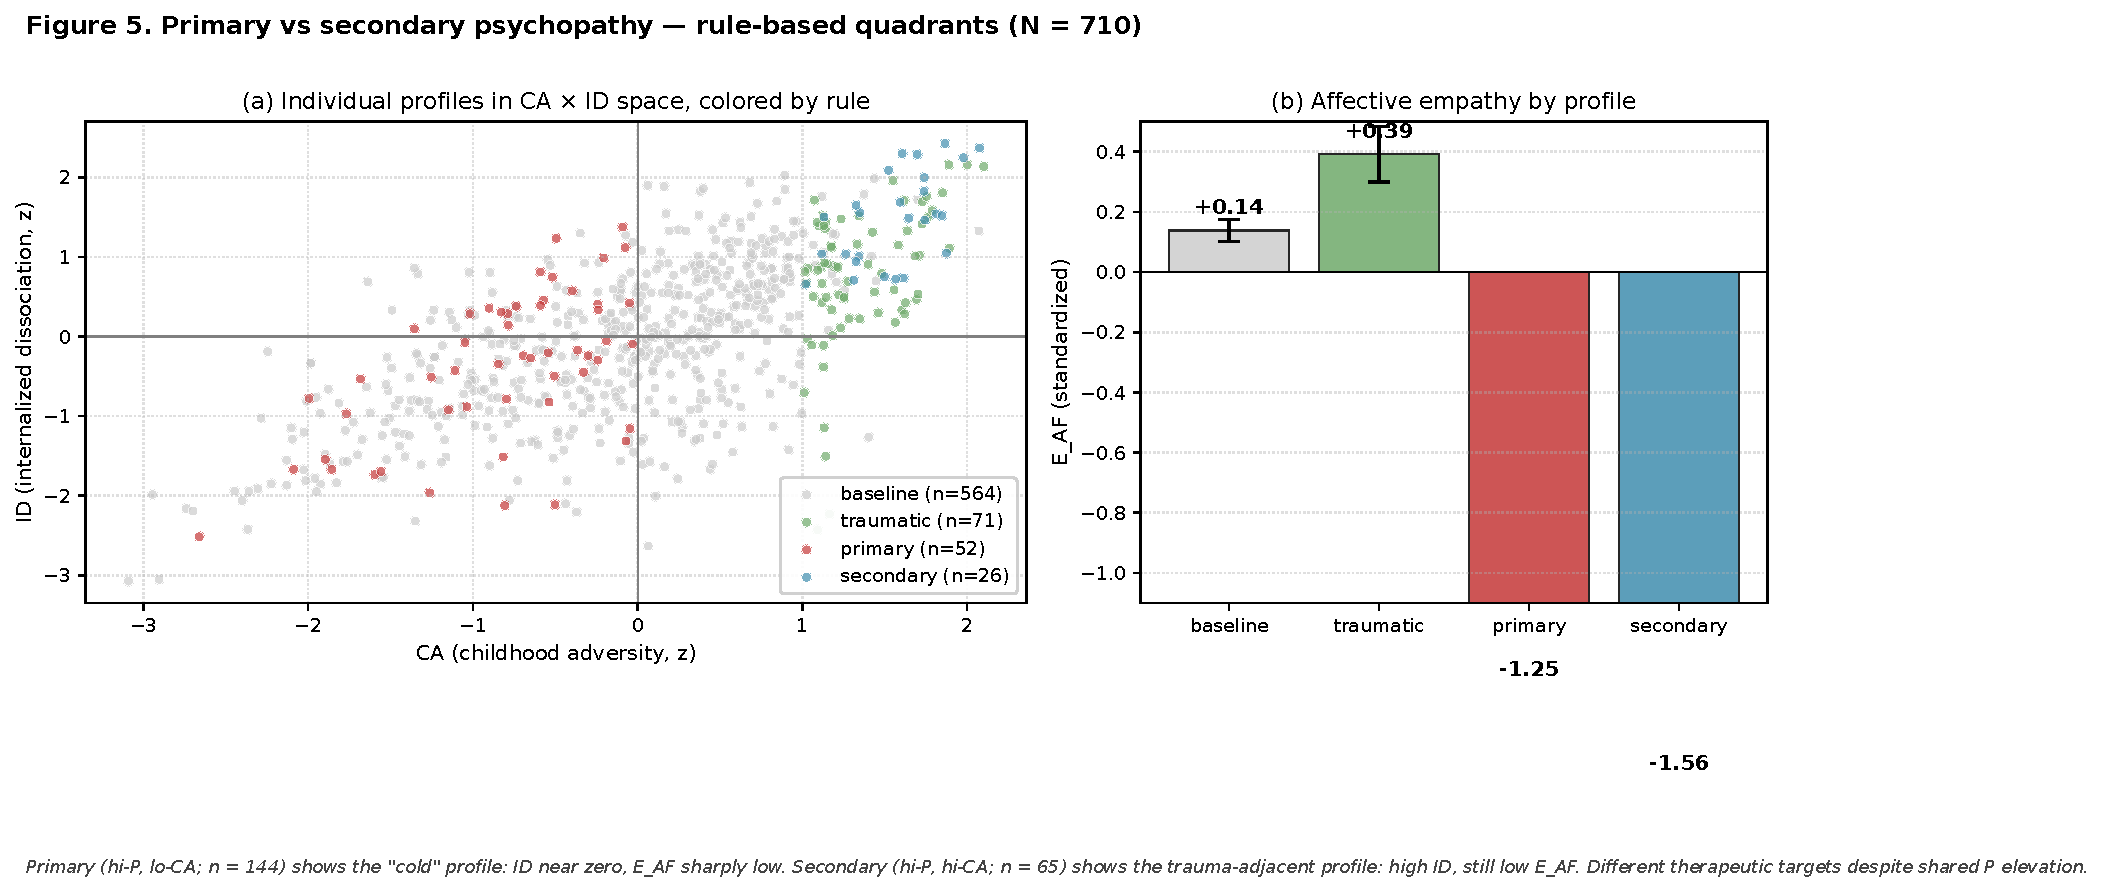
\includegraphics[width=0.9\textwidth]{figures/fig5_primary_secondary.pdf}
\caption{Primary vs secondary психопатические паттерны: диаметрально различны по ID и CA при сходстве по P и \EAF{}.}
\label{fig:primary_secondary}
\end{figure}

Оба профиля имеют сниженную \EAF{} и повышенную P, но диаметрально различаются по ID и CA. Primary-like --- холодный, без внутреннего конфликта и без травматической истории. Secondary-like --- выраженная травма, выраженный внутренний конфликт, при этом такая же сниженная \EAF{}. ANOVA ID $\times$ профиль: $F(1, 207) = 33.9$, $p = 2.2 \times 10^{-8}$, $\eta^2_p = 0.14$.

\textbf{Клинические следствия} (в §\ref{sec:discussion}): первичный и вторичный паттерны выглядят идентично на уровне поведения, но требуют разных терапевтических стратегий. Без измерения ID и CA эти два кластера неразличимы в стандартной поведенческой оценке. Размер secondary-like ($N = 65$) ограничивает точность величин эффектов --- отмечено в §\ref{sec:limitations}.

\paragraph{Сходимость с существующей психометрией (LSRP).} Полученная топология не противоречит, а уточняет двухфакторную структуру Levenson Self-Report Psychopathy Scale~\citep{levenson1995}. LSRP извлекает Factor~1 (primary: callousness, manipulation, self-interest) и Factor~2 (secondary: impulsivity, short-term gratification, anxiety-linked) как \emph{статически-корреляционное} разделение айтемов внутри P-шкалы. Наша $2 \times 2$-топология даёт \emph{этиологическую} координату того же разделения: primary-like (близко к LSRP Factor~1) --- P при $\text{ID} \approx 0$ и $\text{CA} \approx 0$, то есть архитектурный P, ортогональный детской истории; secondary-like (близко к LSRP Factor~2) --- P при $\text{ID} \approx +0.90$ и $\text{CA} \approx +0.98$, то есть травма-порождённый P с активным внутренним конфликтом. Левенсон описал различие статически и предположил его karpman'овскую природу; DEIC-координаты позволяют увидеть, \emph{какой каскад} стоит за каждым из факторов и почему они требуют разных клинических маршрутов. Это --- convergent validation: независимый инструмент с другой теоретической рамкой извлекает ту же двухкомпонентную структуру; DEIC дополняет его механизмом её происхождения.

\subsection{A как формативный конструкт: A-CFA}
\label{subsec:a_cfa}

\subsubsection{Tier 5 --- три варианта single-factor reflective A}

Систематическая проверка: может ли A быть валидирован как единый латентный рефлексивный фактор в текущем инструменте?

\begin{itemize}
    \item \textbf{Full model} (все 31 A-взвешенных айтемов): CFI~=~0.556, RMSEA~=~0.112, $\omega = 0.484$. Выраженный fail; модель не может собрать 31 айтем из 9 разных шкал в единый фактор.
    \item \textbf{Core model} (айтемы с $|w_A| \geq 0.3$, $n = 18$): CFI~=~0.606, RMSEA~=~0.142, $\omega = 0.908$. Надёжность высокая, но fit неприемлемый.
    \item \textbf{Purest model} (17 метакогнитивных self-observation айтемов): CFI~=~0.866, RMSEA~=~0.081; $\omega_{\text{signed}} = 0.186$, $\omega_{\text{abs}} = 0.947$ (корректная интерпретация при биполярных нагрузках).
\end{itemize}

Fit маргинальный, но близкий к acceptable. Однако загрузки биполярны: 8 айтемов грузят в одну сторону, 9 --- в противоположную, несмотря на априорное polarity alignment.

\subsubsection{Tier 5b --- two-factor CFA на purest-17}

Биполярность мотивировала раздельное моделирование двух наблюдаемых кластеров:
\begin{description}
    \item[A\_presence ($n = 8$):] содержание --- позитивная феноменология присутствия («я ясно ощущаю эмоции», «я в контакте с собой», «я проживаю свои чувства»).
    \item[A\_absence ($n = 9$):] содержание --- феноменология диссоциации и онемения («всё как во сне», «я не помню, что чувствовал», «я замираю внутри»).
\end{description}

Two-factor CFA: CFI~=~0.883, RMSEA~=~0.076; $\omega_{\text{abs}}$(A\_presence) = 0.879, $\omega_{\text{abs}}$(A\_absence) = 0.950; $r$(A\_presence, A\_absence) = $+0.355$. Two-factor fit маргинально лучше single-factor ($\Delta$CFI = $+0.017$, $\Delta$RMSEA = $-0.005$), но улучшение не драматично. Критически: факторная корреляция $r = +0.355$ --- умеренная положительная, далеко от единицы. Это психометрически различимые конструкты, не один.

\subsubsection{Latent A в conditional process SEM: sign-reversal}

Каждый латентный A подставлен в тот же conditional process SEM, что и композит (Таблица~\ref{tab:a_signflip}).

\begin{table}[htbp]
\centering
\caption{Sign-reversal при переходе от композита к латентным моделям A.}
\label{tab:a_signflip}
\small
\begin{tabular}{lrrrr}
\toprule
Модератор & $a_{\text{mod}}$ & $b_{\text{mod}}$ & \IMM{} & Значим? \\
\midrule
Композит \texttt{mapped\_attention} & $-0.033$ & $+0.060$ & $\mathbf{-0.00197}$ & \textbf{Да} \\
Latent A (Tier 5 purest) & $+0.018$ & $-0.024$ & $-0.00044$ & Нет \\
Latent A\_presence (Tier 5b) & $-0.013$ & $+0.026$ & $-0.00034$ & Нет \\
Latent A\_absence (Tier 5b) & $-0.020$ & $+0.023$ & $-0.00048$ & Нет \\
\bottomrule
\end{tabular}
\end{table}

Знаки ключевых коэффициентов переворачиваются при переходе от композита к латентным моделям. В композите $\beta_{A_{\text{ID}}} = -0.626$; в latent models --- от $+0.659$ (Tier 5 purest) до $-0.689$ (Tier 5b A\_absence). Direction сильно зависит от того, \emph{какую часть} A-пространства мы моделируем.

Этот sign-flip --- не артефакт анализа, а эмпирическая демонстрация того, что теоретически взвешенный композит ловит иной конструкт, чем голый латентный фактор из метакогнитивной подгруппы айтемов. Композит \emph{включает} айтемы из E, P, CA, EC-шкал с их теоретическими весами; совокупность этих включений ловит модерирующий сигнал. Метакогнитивная подгруппа --- меньший подпространство A-функции; её латентный фактор не воспроизводит сигнал.

\textbf{Содержательная интерпретация:} в текущем инструменте witnessing-функция не локализована в подмножестве метакогнитивных айтемов. Она распределена по пространству вопросов инструмента с дифференциальными теоретическими весами. A как формативный конструкт корректен; A как рефлексивный латентный конструкт --- несовместим с текущим item pool. Разработка dedicated A-scale с айтемами, специально дизайнированными как рефлексивные индикаторы witnessing, --- приоритет первой очереди (§\ref{sec:future}).

Это результат, который мы выносим в статью не как оговорку, а как часть основного findings: он демонстрирует формативную природу A прямо, и обосновывает следующий шаг программы исследований.

\subsection{ID как bifactor: структура внутри пассивного блокирования}
\label{subsec:id_bifactor}

Публикуемая шестифакторная oblique CFA использует один латент \textbf{ID}, объединяющий пять wave-1 шкал пассивного блокирования: концептуальный центр \texttt{IDS} (\emph{Internal Dissonance Scale}, внутренний диссонанс) и четыре mechanism-specific шкалы --- \texttt{SUP} (Suppression, подавление), \texttt{DIS} (Dissociation, диссоциация), \texttt{AIS} (Affective Isolation Scale, аффективная изоляция) и \texttt{FLA} (Flattening, аффективная уплощённость). Решение о сворачивании в единый латент --- содержательное и парсимониальное; отдельный анализ показывает, что структура внутри ID не полностью одномерна, и это эмпирически важный факт для волны~2.

\paragraph{Спецификации.} На пятнадцати parcel'ах (три parcel'а на каждую из пяти защитных шкал, $N = 1426$, данные z-scored) сравнены три модели: \textbf{(i)}~unidimensional --- один латент ID, 15 parcel'ов; \textbf{(ii)}~oblique 5-factor --- пять коррелированных латентов IDS, SUP, DIS, AIS, FLA; \textbf{(iii)}~bifactor --- один общий латент ID\textsubscript{g} плюс пять ортогональных specific-factors (s\textsubscript{IDS}, s\textsubscript{SUP}, s\textsubscript{DIS}, s\textsubscript{AIS}, s\textsubscript{FLA}), с ID\textsubscript{g} ортогонален каждому из specifics.

\paragraph{Сравнение моделей.} Unidimensional не проходит конвенциональные пороги: $\chi^2(90) = 1143.3$, CFI~=~0.829, TLI~=~0.801, RMSEA~=~0.091. Oblique 5-factor сходится, но фит маржинальный: $\chi^2(80) = 750.0$, CFI~=~0.891, TLI~=~0.857, RMSEA~=~0.077; при этом латентные корреляции между пятью шкалами имеют $|r| = 0.66$--$0.89$ с частично противоположными знаками, то есть структура проявляет симптомы полу-свёрнутой коллинеарности. Bifactor фитится значимо лучше обоих: $\chi^2(75) = 536.7$, CFI~=~0.925, TLI~=~0.895, RMSEA~=~0.066, SRMR ниже и AIC~=~89.2 против 58.4 (unidimensional) и соответствующих значений 5-factor (обе вложены). $\Delta\chi^2$ (unidimensional $\to$ bifactor) $= 606.6$ на $15$ df, $p \ll 0.001$: добавление subscale-specific дисперсии статистически неизбежно.

\paragraph{ECV и $\omega_h$.} Метрики бифактора информативнее глобального fit'а. Общая факторная дисперсия (ECV\textsubscript{global}) $= 0.571$ --- общий ID объясняет 57\% общей дисперсии, доступной на parcel-уровне. Hierarchical omega $\omega_h = 0.651$: при использовании полной композитной шкалы ID 65\% надёжной дисперсии отражает общий конструкт, 35\% --- subscale-specific остаточное. $\omega_{\text{total}} = 0.806$.

\paragraph{Per-subscale ECV: гетерогенность поглощения.} Per-subscale ECV $=$ доля дисперсии подшкалы, объясняемая общим ID, остальное идёт на subscale-specific:

\begin{center}
\begin{tabular}{lcc}
\hline
Wave-1 subscale & ECV\textsubscript{sub} & Интерпретация \\
\hline
IDS (Internal Dissonance) & 0.66 & хорошо поглощается общим ID \\
FLA (Flattening) & 0.86 & почти полностью поглощается \\
DIS (Dissociation) & 0.54 & умеренное разделение \\
AIS (Affective Isolation) & 0.53 & умеренное разделение \\
SUP (Suppression) & 0.31 & \textbf{преимущественно отдельный конструкт} \\
\hline
\end{tabular}
\end{center}

\paragraph{Содержательная интерпретация.} SUP --- подавление --- эмпирически не ведёт себя как часть пассивного блокирования. 69\% его дисперсии после bifactor'а остаётся уникальной; композитная корреляция SUP $\leftrightarrow$ IDS составляет всего $r = 0.05$, SUP $\leftrightarrow$ DIS $= 0.11$. Феноменологически это согласуется с тем, что подавление --- эго-синтонное сознательное действие (субъект \emph{выбирает} не чувствовать), в отличие от диссоциации, изоляции, уплощённости --- автоматических, эго-дистонных механизмов. Напротив, FLA почти полностью поглощается общим ID (86\%) --- аффективная уплощённость эмпирически есть та же структура, что IDS, просто видимая на другой поверхности. DIS и AIS держат около половины уникальной дисперсии --- нуждаются в уточнённых айтемах для чистой сепарации.

\paragraph{Операциональное следствие.} Публикуемая унифакторная ID сохраняется как парсимоничная структура для основных предсказаний статьи и для conditional process SEM; она поддерживается всеми последующими анализами (a-путь CA$\to$ID, b-путь ID$\to$\EAF{}, A-модерация), потому что эти предсказания касаются общей ID-дисперсии. Bifactor-результат --- основание для двух изменений в волне~2: \textbf{(a)}~SUP с высокой вероятностью должен быть отдельным латентом, не субшкалой ID; \textbf{(b)}~публикуемая модель в волне~2 может быть bifactor по умолчанию, с IDS и FLA как почти чистыми индикаторами общего ID и DIS/AIS как mixed-loaded индикаторами. Редизайн пяти защитных шкал под эту структуру развёрнут в §\ref{subsec:wave2_design}.

\begin{figure}[htbp]
\centering
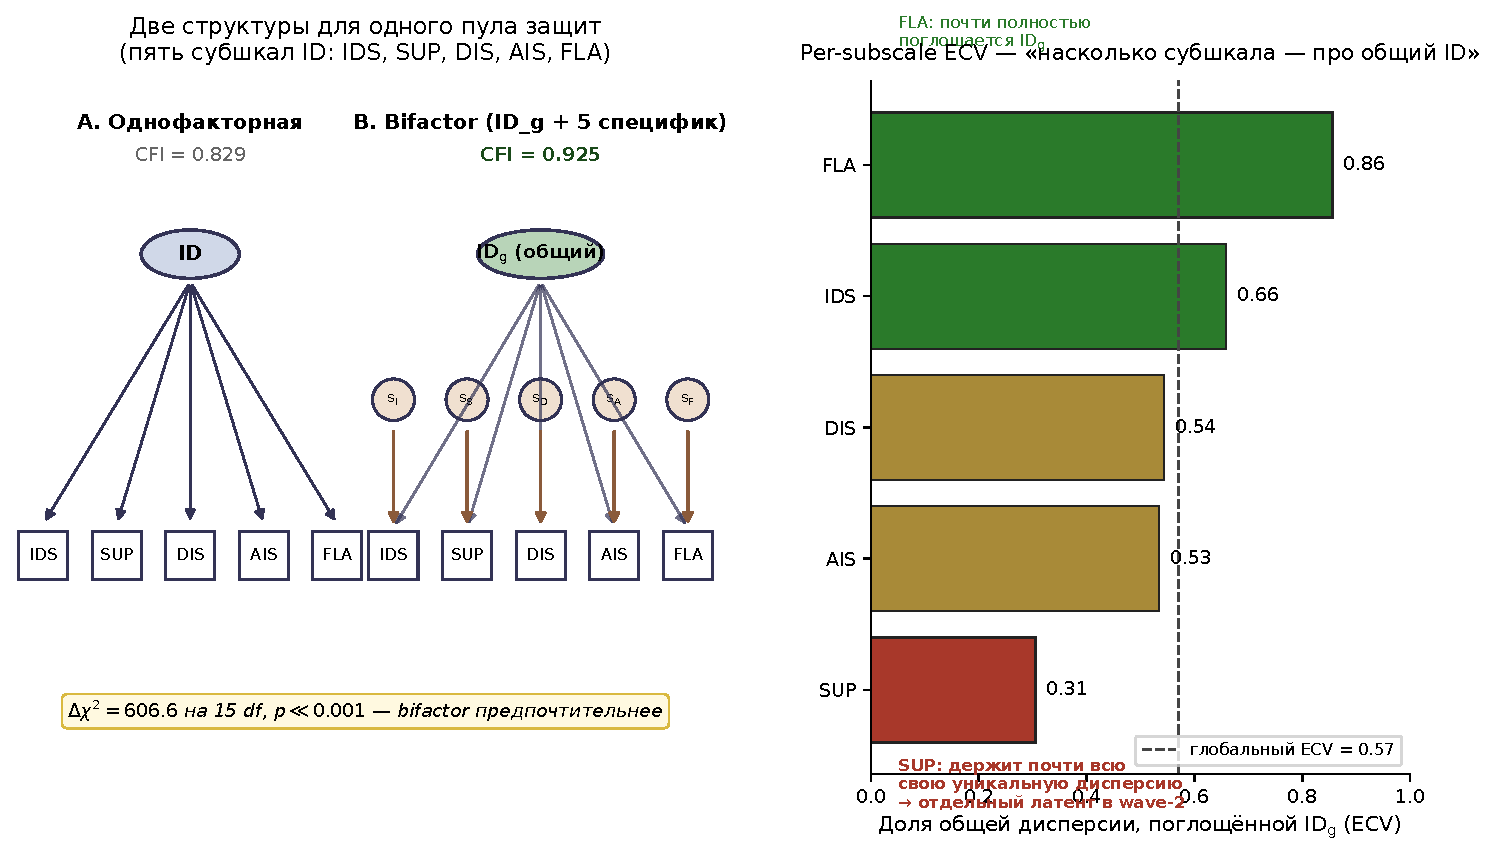
\includegraphics[width=0.95\linewidth]{figures/fig8_bifactor_structure.pdf}
\caption[Бифакторная структура ID]{Бифакторная структура ID. Панель (а): схематическое сравнение однофакторной модели (единый латент ID, все пять шкал --- его прямые индикаторы) с бифакторной моделью (общий ID\textsubscript{g} плюс пять ортогональных specific-факторов s\textsubscript{IDS}, s\textsubscript{SUP}, s\textsubscript{DIS}, s\textsubscript{AIS}, s\textsubscript{FLA}); $\Delta\chi^2 = 606.6$ на 15 df, $p \ll 0.001$. Панель (б): per-subscale ECV --- доля дисперсии шкалы, поглощаемая общим ID-фактором. Пунктирная линия показывает ECV\textsubscript{global}~=~0.571. FLA и IDS почти полностью поглощаются общим ID; SUP сохраняет 69\% уникальной дисперсии и требует отдельного латента в волне~2.}
\label{fig:id_bifactor}
\end{figure}

Численные сводки --- в \texttt{id\_bifactor\_summary.json} (fresh\_analysis).

\subsection{Клиническая гетерогенность канала CA$\to$ID$\to$\EAF{}}
\label{subsec:clinical_subgroup_patterns}

Параллельная медиация §\ref{subsubsec:parallel_mediation} даёт усреднённую картину по всей выборке. Клинически значимый вопрос --- распадается ли этот усреднённый канал на различимые паттерны внутри нозологических подгрупп, собранных по самоописанию в свободном поле (§\ref{subsec:free_text_convergent}). Мы запустили ту же спецификацию ($\mathrm{CA} \to \mathrm{ID} \to E_{\mathrm{AF}}$, без $A$) отдельно в четырёх самых частых кластерах: trauma\_disorder ($n=57$), personality\_disorder/BPD ($n=128$), mood\_disorder ($n=158$), selfharm\_mention ($n=129$); плюс контрольная подвыборка респондентов без единого текстового диагностического флага ($n=1040$). Подгруппы пересекаются, поэтому цифры следует читать как характеристику паттерна, а не как формально независимые тесты.

\begin{table}[htbp]
\centering
\small
\caption[Четыре клинических паттерна канала CA$\to$ID$\to$\EAF{}]{Параметры параллельной медиации в четырёх клинических подгруппах и контрольной подвыборке. $c$ --- total effect CA на \EAF{}, $c'$ --- direct effect после контроля ID, $a \cdot b$ --- indirect через ID. Суппрессор определяется как $\mathrm{sign}(c) \neq \mathrm{sign}(c')$.}
\label{tab:clinical_subgroup_patterns}
\begin{tabular}{lrrrrrl}
\hline
Подгруппа & $n$ & $c$ & $c'$ & $a \cdot b$ & Суппрессор & Паттерн \\
\hline
Полная выборка & 1551 & $-0.103$ & $+0.122$ & $-0.225$ & yes & baseline \\
No-diagnosis & 1040 & $-0.121$ & $+0.114$ & $-0.234$ & yes & baseline (здоровые) \\
Trauma disorder & 57 & $+0.033$ & $+0.077$ & $-0.044$ & no & инвертированный \\
Personality/BPD & 128 & $-0.046$ & $+0.191$ & $-0.237$ & yes & оба канала выражены \\
Mood disorder & 158 & $-0.179$ & $+0.021$ & $-0.199$ & борд. & блокировочный \\
Selfharm mention & 129 & $+0.023$ & $+0.251$ & $-0.229$ & no & сенсибилизация внутрь \\
\hline
\end{tabular}
\end{table}

Три содержательных наблюдения. \emph{Во-первых}, в подгруппе без единого текстового диагноза ($n=1040$) коэффициенты практически тождественны полной выборке. Суппрессор-эффект CA$\to$ID$\to$\EAF{} --- не артефакт клинического подсэмпла: он присутствует с той же амплитудой в условно-здоровой части выборки. Это отвечает на стандартный критический вопрос «не это ли особенность травмированных?» эмпирически: не особенность. \emph{Во-вторых}, четыре клинических подгруппы дают четыре \emph{качественно разных} профиля. PTSD (trauma disorder, $n=57$): суппрессор исчезает, total-эффект CA$\to$\EAF{} становится слабо-положительным, $a$-путь $\mathrm{CA}\to\mathrm{ID}$ ослаблен ($a = 0.27$ против $0.43$ в полной выборке). Травматический материал в этой подгруппе не заблокирован до конца --- он «торчит наружу» как аффективная сверхчувствительность. Это совместимо с клинической картиной PTSD как неинтегрированной гипер-reactivity, в т.ч. в сторону эмпатии. BPD/личностные ($n=128$): самый сильный положительный $c'$ ($+0.191$) при сильной блокировке ($b = -0.59$); сосуществует выраженная сенсибилизация и выраженная диссоциация --- классический пограничный профиль. Mood disorder ($n=158$): total $c = -0.179$, direct $c' \approx 0$; в депрессии CA действует почти исключительно через блокировку, прямой сенсибилизирующий канал гасится --- согласуется с клинической моделью депрессии как выключения аффективных резонансов. Selfharm ($n=129$): самый большой положительный direct $c'$ ($+0.251$); эмпатическая боль выходит из-под контроля внутрь, а не в сторону другого человека.

\emph{В-третьих}, сам факт, что один и тот же структурный канал даёт четыре разных клинических паттерна, --- это эмпирическое основание для предсказания дифференциального ответа на траума-targeted вмешательства (§\ref{subsec:clinical}): интегрированная работа с защитной структурой наиболее полезна там, где канал $b$ активен и сенсибилизация видима в $c'$ (BPD, selfharm); в PTSD первичная задача --- метаболизация неинтегрированного материала, не его извлечение из-под блокировки; в депрессии первичная задача --- работа с блокировкой как таковой, до того как прямой канал сможет заработать.

\subsection{Биполярное расстройство как natural experiment}
\label{subsec:bipolar_experiment}

Биполярная подгруппа ($n=51$, упоминание BD~I/II в свободном поле) даёт частный случай, который не укладывается ни в один из четырёх паттернов выше и представляет отдельный теоретический интерес. В этой подгруппе классический suppressor исчезает в противоположном направлении: direct-путь CA$\to$\EAF{} не просто переживает суппрессор --- он доминирует над indirect-путём ($c' = +0.404$, $p < 10^{-4}$; $a \cdot b = -0.257$; total $c = +0.147$, ns), и общий эффект CA на \EAF{} становится положительным (хотя на $n=51$ не достигает значимости, $p = 0.13$). Для сравнения, во всей остальной выборке без BD ($n=1500$) direct-путь $c' = +0.114$, то есть в BD direct-путь усилен почти в четыре раза.

Содержательная интерпретация: в подгруппе с биполярной архитектурой ранний адверсивный опыт не блокируется до нуля, а, напротив, прямо усиливает аффективную эмпатию, минуя защитный контур. Это согласуется с клиническими описаниями гипоманической фазы как «выжигающе эмпатической» и с идентификационным механизмом, при котором травматический материал ассимилируется как личный аффективный ресурс, а не как угроза, требующая защиты. Для дальнейшей работы этот паттерн --- кандидат на отдельный предикторный каркас: BD как architecture-level модератор канала CA$\to$\EAF{}, ортогональный стандартной оси ID.

Ограничения: $n=51$, самоидентификация без формальной верификации DSM, выборка несёт selection bias в сторону психически чуткой популяции. Значимость direct-эффекта $c'$ устойчива к этим ограничениям ($p < 10^{-4}$), total-эффект $c$ --- нет. Аккуратная формулировка: внутри биполярной подгруппы структура канала \emph{качественно иная}, не \emph{количественно другая}.

\subsection{Гендер-стратификация: суппрессор универсален, но амплитуда $b$ зависит от пола}
\label{subsec:gender_moderation}

Суппрессор воспроизводится в обоих гендерных подвыборках ($n_\mathrm{жен} = 932$, $n_\mathrm{муж} = 356$): total $c$ отрицателен, direct $c'$ положителен, indirect через ID сильно отрицателен в обеих. Амплитуда $b$ различается: формальный тест гендер-модерации в объединённой выборке ($n = 1288$) даёт $\mathrm{D}\times\mathrm{male} \; \beta = +0.189$, $p = 0.002$ --- то есть у мужчин связь $\mathrm{D} \to E_{\mathrm{AF}}$ \emph{слабее} (отрицательный наклон менее крутой), чем у женщин. Гендер-интеракция с CA незначима ($\beta = -0.04$, $p = 0.42$), структура канала $a$ не отличается.

Интерпретация сдержанная: суппрессор как механизм универсален; количественный параметр $b$, то есть сила, с которой присутствие защитной архитектуры подавляет аффективную эмпатию, у мужчин несколько меньше. Возможных содержательных объяснений несколько: (а) у мужчин в среднем меньше социального давления «показать эмпатию», поэтому даже при высокой D они не показывают максимально возможного падения E\textsubscript{AF}, а наоборот --- их базовая E\textsubscript{AF} уже ниже, и падать некуда; (б) у женщин E\textsubscript{AF}-базовая выше, поэтому абсолютный перепад под действием D виднее. Мы не можем различить эти два объяснения на single-wave данных. Но ключевое: гендер-эффект --- параметрический, не структурный. Включать пол в основную модель как ковариату не обязательно; суппрессор сохраняет значимость и направление в обоих стратах.

\subsection{Возрастная инвариантность суппрессора (формальные числа)}
\label{subsec:age_invariance_numbers}

Гипотеза «суппрессор --- стадия развития, исчезающая с возрастом» формально отвергается. Мы разбили выборку на шесть возрастных бинов (14--20, 20--25, 25--30, 30--35, 35--45, 45--65) и запустили спецификацию CA$\to$ID$\to$\EAF{} с контролем $A$ отдельно в каждом бине.

\begin{table}[htbp]
\centering
\small
\caption[Параметры суппрессора по возрастным бинам]{Параметры медиации CA$\to$ID$\to$\EAF{}|$A$ в шести возрастных бинах. $a$ --- путь CA$\to$ID, $b$ --- путь ID$\to$\EAF{} с контролем $A$, $c$ --- total, $c'$ --- direct, $a \cdot b$ --- indirect. Суппрессор: $\mathrm{sign}(c) \neq \mathrm{sign}(c')$.}
\label{tab:age_bins_suppressor}
\begin{tabular}{lrrrrrrc}
\hline
Бин & $n$ & $a$ & $b$ & $c$ & $c'$ & $a\cdot b$ & Суппрессор \\
\hline
14--20 & 217 & $+0.40$ & $-0.65$ & $-0.08$ & $+0.18$ & $-0.26$ & yes \\
20--25 & 437 & $+0.39$ & $-0.50$ & $-0.06$ & $+0.14$ & $-0.20$ & yes \\
25--30 & 334 & $+0.45$ & $-0.58$ & $-0.19$ & $+0.07$ & $-0.26$ & yes \\
30--35 & 181 & $+0.49$ & $-0.54$ & $-0.14$ & $+0.12$ & $-0.26$ & yes \\
35--45 & 131 & $+0.39$ & $-0.42$ & $-0.01$ & $+0.16$ & $-0.17$ & yes \\
45--65 & 38 & $+0.37$ & $-0.01$ & $-0.16$ & $-0.16$ & $0.00$ & no (мал $n$) \\
\hline
\end{tabular}
\end{table}

Коэффициенты $a$ ($\mathrm{CA}\to\mathrm{ID}$) и $b$ ($\mathrm{ID}\to E_{\mathrm{AF}}$) структурно стабильны от 14 до 45 лет: $a \in [+0.39, +0.49]$, $b \in [-0.65, -0.42]$. Формальный тест в объединённой выборке ($n = 1340$, 14--45): $\mathrm{young}(<25) \times \mathrm{D} \to E_{\mathrm{AF}} \; \beta = -0.01$, $p = 0.75$ --- амплитуда $b$ не отличается между молодыми и взрослыми. Единственное слабое отклонение: $\mathrm{young} \times \mathrm{CA} \to E_{\mathrm{AF}} \; \beta = +0.04$, $p = 0.08$ --- у молодых прямой положительный путь CA$\to$\EAF{} несколько «обнажённее», возможно потому, что компенсаторный защитный слой ещё не до конца собран. Последний бин 45--65 ($n = 38$) теряет эффект, но это, скорее всего, эффект малой и смещённой выборки (респонденты 45+ с низким ACE и низкой D, floor-эффект). Интерпретировать это как «суппрессор проходит с возрастом» было бы неверно; формально тест $\mathrm{D}\times\mathrm{age}$ не проходит на объединённых данных.

Следствие для теоретического каркаса: суппрессор --- не стадия развития, а структурный механизм, сложившийся до подросткового возраста и сохраняющийся при измерении от 14 до 45 лет. В сочетании с тем, что $P$-шкала не меняется с возрастом ($\beta = -0.007$, $p = 0.60$, $R^2 = 0.0002$), а $D$-score систематически снижается ($\beta = -0.055$, $p < 10^{-7}$, $R^2 = 0.021$), складывается дихотомия: $P$ ведёт себя как чистый trait (стабильный во времени), $D$ --- как state-like индекс, амплитуда которого со временем ослабевает при сохранении той же структурной связи с CA и \EAF{}. Это согласуется с клиническим наблюдением, что защитная архитектура, раз сложившись, остаётся, но её манифестация смягчается --- либо через интеграцию (высокий $A$), либо просто через усталость со временем.

\subsection{Конвергентная валидация через свободное поле}
\label{subsec:free_text_convergent}

Из $N = 1426$ респондентов $511$ заполнили необязательное свободное поле с описанием своего психического опыта (диагнозы, симптомы, лечение, самонаблюдения). Тексты категоризированы автоматически по регулярным выражениям, покрывающим нозологии DSM, упоминания терапии и медикаментов, а также тринадцать дополнительных поведенческих осей (манипулятивность/холодность, поиск ощущений, социальная изоляция, проблемы контроля агрессии, употребление рекреационных веществ, описания ремиссии, и др.). Анализ предоставляет независимый, не зашумлённый латентной автокорреляцией шкал, срез конвергентной и дискриминантной валидности конструкта. Мы выделяем три содержательно приоритетных результата.

\paragraph{Прямое подтверждение P-шкалы через самоописание.} Десять респондентов описали себя в свободном поле через термины «манипулятивность», «патологическая ложь», «макиавеллизм», «холодная расчётливость», «психопатические черты», «социопатия». На композитной P-шкале они находятся в $+2.32$ SD над базой ($p = 4.8 \times 10^{-6}$), на E-шкале --- в $-1.48$ SD под базой ($p = 6.1 \times 10^{-7}$). В логистической регрессии «член ли категории manipulation\_callousness» с полным набором ковариат (E, A, Lie, ACE, D), $z$-стандартизованных, коэффициент $\beta_P = +1.66$ ($p = 0.003$) --- то есть P удерживает значимость после контроля всех альтернативных объяснений. AUC полной модели $= 0.968$; AUC одной P-шкалы $= 0.964$. Это --- прямое convergent подтверждение P-шкалы через независимое текстовое самоописание: люди, которые \emph{узнают} себя в словаре холодного инструментализма, получают от инструмента тот же структурный профиль, который конструкт предписывает. В контексте 131-пунктового инструмента, построенного worldview-first (§\ref{subsec:worldview_first}), это одно из самых сильных эмпирических свидетельств, что P-шкала измеряет то, что она называется.

\paragraph{Архитектурная диссоциация P \emph{vs} ID через поведенческие якоря.} Следующий логический шаг --- проверить, разделимы ли два канала (активный P и пассивный ID) на уровне поведенческих маркеров, а не только на уровне латентных конструктов в SEM. Мы прогоняем логистические регрессии «член ли категории X» для семи поведенческих флагов с единым набором ковариат \{E, A, Lie, ACE, D\}, $z$-стандартизованных. После полного контроля чистую специфичность сохраняют ровно два полюса:

\begin{center}
\begin{tabular}{lccc}
\toprule
Флаг & $N^+$ & $\beta_P$ ($p$) & $\beta_D$ ($p$) \\
\midrule
\textbf{manipulation\_callousness} & 10 & $\mathbf{+1.66}$ (0.003) & $-0.88$ (0.13) \\
\textbf{social\_isolation}          &  9 & $-0.69$ (0.17)          & $\mathbf{+1.41}$ (0.034) \\
sensation\_seeking                 & 25 & $+0.37$ (0.22)          & $+0.49$ (0.21) \\
aggression\_control                & 14 & $+0.37$ (0.29)          & $+0.61$ (0.23) \\
recreational\_drug                 & 22 & $-0.41$ (0.23)          & $+0.22$ (0.60) \\
bipolar                            & 51 & $+0.24$ (0.25)          & $-0.21$ (0.43) \\
\bottomrule
\end{tabular}
\end{center}

Остальные пять флагов после контроля ковариат теряют специфичность --- их bivariate связи с P и D объясняются общей вариацией E/A/ACE. Это не слабость шкал, а ожидаемая структура: поведенческие флаги разнородны и содержат смешанные сигналы. Чистая диссоциация сохраняется на \emph{полюсах}: manipulation\_callousness активирует P-канал без активации ID-канала; social\_isolation активирует ID-канал без активации P-канала. Это независимое behavioral-anchor подтверждение диссоциации, постулированной в §\ref{subsubsec:parallel_mediation} на уровне latent SEM.

\paragraph{Содержательные эффекты на bivariate уровне.} Остальные категории не проходят multivariate-контроль, но несут содержательный signal bivariate, который уточняет портрет каждого канала:

\begin{center}
\begin{tabular}{lcccc}
\toprule
Категория ($N^+$) & $d_P$ & $d_D$ & $d_E$ & $d_A$ \\
\midrule
manipulation\_callousness ($10$)   & $+2.32$ & $+0.55$ & $-1.48$ & $-0.63$ \\
sensation\_seeking ($25$)          & $+0.55$ & n.s.    & n.s.    & n.s.    \\
social\_isolation ($9$)            & n.s.    & $+0.80$ & n.s.    & $-0.61$ \\
aggression\_control ($13$)         & n.s.    & $+0.59$ & n.s.    & n.s.    \\
recreational\_drug ($22$)          & n.s.    & n.s.    & n.s.    & $+0.49$ \\
remission\_past ($52$)             & n.s.    & n.s.    & n.s.    & n.s.    \\
\bottomrule
\end{tabular}
\end{center}

Три наблюдения. Первое: sensation\_seeking даёт чистый $+P$ без $+D$ --- классический Cleckley-компонент (поиск ощущений, импульсивность без глубокого аффективного нарушения) воспроизводится в $+P$, не в $+D$. Это эмпирически поддерживает теоретическое различение активной P-архитектуры условного доступа и пассивной ID-блокировки. Второе: aggression\_control даёт $+D$, $+$ACE, но не $+P$ --- реактивная агрессия, в отличие от инструментальной, принадлежит ID-контуру, не P-контуру. Это согласуется с многолетней клинической картиной «affective vs predatory aggression». Третье: recreational\_drug (каннабис, психоделики) даёт единственный эффект на A ($d = +0.49$), что согласуется с mindfulness-enhancing литературой; направление каузальности self-report здесь не устанавливает.

\paragraph{Второй путь к интегрированному выжившему: remission\_past $+$ hi-A.} Анализ §\ref{subsec:integrated_survivor} операционализировал интегрированного выжившего через rule-based 2$\times$2 (CA-hi $\times$ A-hi), независимо от текстовых данных. Свободное поле даёт второй, текст-якорный маршрут к тому же профилю: среди $511$ заполнивших свободное поле, $52$ упомянули свой статус как «в ремиссии», «прошло $N$ лет без», «в прошлом». Пересечение этих $52$ с группой A в верхнем терциле даёт $N = 16$. Контраст integrated ($N = 16$) против stuck ($N = 188$, hi-ACE $\times$ lo-A в остальной выборке): D-компоненты $d = -1.5 \dots -2.7$, E $d = +1.35$, ACE $d = -1.45$. Контраст integrated против базы (never-dx, lo-A, $N = 321$): D-компоненты $d \approx -2.3$, E $d = +1.81$, ACE $d = -0.93$. Иначе говоря, интегрированная подгруппа по защитным шкалам располагается \emph{ниже} базы, по эмпатии --- \emph{выше} базы; это не «возврат к норме», это движение через точку базы в противоположный край. Caveats: $N = 16$ мало для SEM-валидации; сниженный ACE относительно stuck допускает self-selection (более мягкий детский фон --- выше вероятность дойти до интеграции), а не чистый эффект recovery. Но сама направленность согласуется с rule-based 2$\times$2-результатом и усиливает его через независимую выборку.

\subsection{Дискриминантная валидность: ROC по self-reported диагнозам}
\label{subsec:roc_validity}

Дополнительный срез валидности --- ROC-характеристики каждой шкалы как предиктора отдельных self-reported нозологических категорий ($N^+$ per category варьирует от $22$ до $158$). Результаты сведены ниже (AUC; значимые $> 0.65$ выделены; $< 0.45$ означает шкала предсказывает \emph{отсутствие} диагноза):

\begin{center}
\small
\begin{tabular}{lccccccc}
\toprule
Диагноз ($N^+$)         & ACE  & CA   & DIS  & ID   & P    & M    & A    \\
\midrule
trauma\_disorder ($56$)      & \textbf{0.76} & \textbf{0.75} & 0.63 & 0.52 & 0.40 & 0.44 & 0.41 \\
self-harm mention ($122$)    & \textbf{0.70} & \textbf{0.70} & 0.67 & 0.58 & 0.40 & 0.49 & 0.36 \\
personality\_disorder ($125$) & \textbf{0.69} & \textbf{0.70} & 0.66 & 0.55 & 0.42 & 0.43 & 0.38 \\
mood\_disorder ($153$)        & 0.60 & 0.61 & 0.60 & 0.50 & 0.38 & 0.41 & 0.42 \\
anxiety\_disorder ($102$)     & 0.58 & 0.58 & 0.56 & 0.49 & 0.37 & 0.42 & 0.46 \\
neurodev ($112$)             & 0.56 & 0.58 & 0.57 & 0.52 & 0.40 & 0.49 & 0.46 \\
substance\_use ($46$)         & 0.54 & 0.60 & 0.58 & 0.52 & 0.50 & 0.42 & 0.39 \\
in\_treatment ($22$)          & 0.60 & 0.60 & 0.58 & 0.51 & 0.42 & 0.42 & 0.43 \\
\bottomrule
\end{tabular}
\end{center}

Три структурных паттерна проявляются сразу. \textbf{Первый:} CA и ACE предсказывают \emph{раннетравматические} клинические кластеры (trauma-disorder, self-harm, personality) с AUC 0.69--0.76. Это ожидаемый паттерн для инструмента, где CA сводит воедино семь индикаторов детской неблагоприятности --- три клинических кластера, для которых эпидемиология показывает сильнейшую связь с детской травмой, получают наибольшую дискриминацию. Для аффективных и тревожных расстройств, которые в современной эпидемиологии частично отвязаны от раннего анамнеза (генетика, нейромедиаторы, ситуативное), CA даёт более слабый, но по-прежнему положительный сигнал (AUC 0.58--0.61). \textbf{Второй:} P во всех восьми dx-категориях даёт AUC $\leq 0.42$. Это означает: P-шкала предсказывает \emph{не} наличие диагноза, а \emph{отсутствие} self-report. Структурно это подпись заблокированной help-seeking --- ровно то, что предсказывает архитектурная интерпретация P: если психический материал субъекта встраивается в нарратив «мне это разрешено, это не болезнь», обращение за формальным диагнозом становится избыточным. P-шкала демонстрирует дискриминантную валидность через противоположное направление --- инструмент \emph{не} ловит P-респондентов через self-report клинического диагноза, и это эмпирическая черта, а не дефект. \textbf{Третий:} A симметрично даёт AUC $\leq 0.46$ для большинства клинических категорий и особенно низкий для self-harm ($0.36$), personality ($0.38$), substance ($0.39$). Высокая А предсказывает \emph{отсутствие} активного клинического диагноза --- это поддерживает чтение А как witnessing-ресурса, а не как нейтральной метакогнитивной способности.

Совокупно три паттерна образуют когерентное доказательство discriminant-валидности: CA работает как трауматический предиктор, P --- как отрицательный предиктор self-report, A --- как симметричный ресурс-предиктор. Эти три подписи не могут сосуществовать в одной шкале случайно.

\paragraph{Редкие dx-категории (не вошедшие в основную ROC-таблицу).} Для полноты картины приводим AUC-значения шести редких категорий, пропущенных в основной таблице из-за низкой базовой частоты: \texttt{dx\_eating\_disorder} ($N = 30$) --- ACE $= 0.69$, CA $= 0.67$ (умеренный трауматический профиль, промежуточный между mood и personality); \texttt{dx\_suicidal\_mention} ($N = 16$) --- ACE $= 0.73$, CA $= 0.74$, DIS $= 0.70$, A $= 0.34$ (канонический высоко-травматический профиль, совместимый с selfharm\_mention); \texttt{dx\_ocd} ($N = 15$) --- относительно baseline (AUC всех шкал 0.39--0.63), без отчётливой архитектурной подписи; \texttt{dx\_on\_medication} ($N = 35$) --- uniform near-baseline (AUC 0.42--0.55), приём медикации не трекает специфической DEIC-оси, что согласуется с §\ref{subsec:free_text_nlp} (med\_mentioned директивно ассоциируется со слегка улучшенным профилем, но эффекты маргинальны); \texttt{dx\_psychotic\_spectrum} ($N = 7$) и \texttt{dx\_dissociative} ($N = 4$) --- слишком редки для формальной интерпретации. Наложение suicidal\_mention ($N = 16$) и selfharm\_mention ($N = 122$): 13 из 16 suicidal-респондентов также флагированы на selfharm; 3 оставшихся --- pure suicidal без упоминания self-harm поведения. В основной ROC-таблице мы агрегируем их под selfharm\_mention для статистической мощности; при $N \geq 300$ в wave-2 эти категории должны быть разведены.

\subsection{\texorpdfstring{Почему \texttt{dx\_count} --- смещённая мера тяжести}{Почему dx_count --- смещённая мера тяжести}}
\label{subsec:dx_count_bias}

Стандартный путь проверки шкалы защит --- её связь с числом self-reported диагнозов, \texttt{dx\_count} (сумма сработавших нозологических категорий в свободном поле, диапазон $0$--$11$). Мы прогоняем этот анализ и формулируем его результат как отдельное методологическое утверждение, а не как footnote к ROC.

$\texttt{dx\_count} \sim D_{\mathrm{score}}$ даёт $R^2 = 0.006$ ($r = +0.078$, $p = 0.08$). То есть агрегированная защитная композита \emph{практически не предсказывает} число диагнозов. $\texttt{dx\_count} \sim \{\mathrm{SUP}, \mathrm{DIS}, \mathrm{AIS}, \mathrm{FLA}, \mathrm{IDS}, M\}$ --- шесть компонент раздельно --- даёт $R^2 = 0.089$. В совместной модели $\texttt{dx\_count} \sim D + E + P$ коэффициент $\beta_P = -0.012$, $p < 0.001$: активный P-профиль ассоциируется с \emph{меньшим} числом диагнозов. ACE$+$CA$+$EC даёт $R^2 = 0.039$ --- раннетравматический анамнез предсказывает \texttt{dx\_count} значительно лучше, чем защитная структура.

Содержательно это означает: \texttt{dx\_count} --- \emph{не} прокси общей тяжести состояния. Он систематически недооценивает hi-P и hi-ID респондентов (первые не считают своё состояние проблемой, вторые блокированы в сторону help-seeking) и монотонно растёт только с раннетравматическим анамнезом, который ведёт к клиническим кластерам, наиболее «видимым» в self-report (trauma, PD, self-harm). Использовать \texttt{dx\_count} как меру тяжести в DEIC-популяции означало бы встроить в модель то самое систематическое смещение, которое архитектура конструкта описывает. Мы поэтому не используем \texttt{dx\_count} как критериальную переменную ни в одном из основных анализов статьи; в §\ref{sec:results} \texttt{dx\_count} фигурирует только как описательная характеристика выборки. Клиническая валидизация и incremental validity над существующими инструментами требуют отдельного wave с формализованной диагностикой (структурированные интервью SCID, MINI), в контролируемой клинической выборке.

Отдельное следствие, выходящее за рамки limitation: если инструмент структурно ловит именно тех, кого self-report системы диагностики \emph{не} ловят, то DEIC-профиль является кандидатом не только на diagnostic-ancillary, но и на первичный screening-tool для под-диагностированной популяции. Формально это collaborative-filtering задача над DEIC-координатами: для нового респондента с неизвестным клиническим статусом предсказывать вероятностный диагностический ландшафт исходя из архитектурной близости к подвыборке с известными диагнозами. Практическая импликация: скрининг на входе в любой контакт с системой помощи (первичка, школьная психологическая служба, университетская медслужба) может флагировать блокированно-травматический и активно-нарративный профили без ожидания самообращения. Эмпирическая проверка выносится в §\ref{sec:future}.

\subsection{Конвергентная валидация через CASE-сценарии}
\label{subsec:case_convergent}

Инструмент содержит $10$ ситуационно-сценарных вопросов (CASE\_1--CASE\_10), каждый с четырьмя поведенчески-контрастными вариантами ответа. В предыдущих версиях анализа они собирались для дескриптивного использования; здесь мы прогоняем их как независимый канал convergent validity для Likert-латентных факторов. Логика теста: если P-, ID- и A-шкалы измеряют то, что они называются, то выбор поведенческого варианта, специально сконструированного как P-сигнатура, должен дифференцировать Likert-P-балл этой подгруппы от остальной выборки, и аналогично для ID- и A-маркированных вариантов. Анализ на $N = 1546$ с валидными CASE-ответами.

\paragraph{CASE\_8: «коллегу уволили по твоей наводке».} Четыре варианта реакции. Два самых экстремальных: \textbf{«Чувствую вину и тревогу»} ($n = 653$; $E = +0.44$, $P = -0.57$, $A = +0.14$, ID $= -0.15$~$\sigma$) и \textbf{«Мне всё равно, главное --- я остался»} ($n = 123$; $E = -1.16$, $P = +1.05$, $A = -0.71$, ID $= +0.46$). Контраст P-signature группы ($n = 358$, включая «он сам виноват» и «мне всё равно») vs остальной выборки: \textbf{$\Delta P = +0.92\,\sigma$, $t$-тест $p = 8 \times 10^{-46}$}; $\Delta E = -0.68\,\sigma$ ($p = 2 \times 10^{-23}$); $\Delta A = -0.25\,\sigma$ ($p = 2 \times 10^{-4}$). Архитектурный профиль точно соответствует тому, что P-шкала предписывает теоретически.

\paragraph{CASE\_10: «выгодно промолчать, чтобы друг попал в неприятности».} Вариант \textbf{«Я промолчу --- не моя проблема»} ($n = 91$) даёт экстремальный дифференциал: $\Delta P = +0.91\,\sigma$ ($p = 3 \times 10^{-10}$), $\Delta E = -1.12\,\sigma$ ($p = 5 \times 10^{-17}$), $\Delta A = -0.71\,\sigma$ ($p = 4 \times 10^{-8}$). Это один из сильнейших единичных behavioral-anchor конвергентных тестов в данных: 91 респондент открыто выбрал вариант преднамеренного причинения вреда другу ради выгоды, и инструмент на независимой Likert-шкале зафиксировал их на ${+}0.86\,\sigma$ по P, ${-}1.05$ по E.

\paragraph{CASE\_1: «пообещал другу, нет ни сил, ни желания».} Вариант \textbf{«Грубо отказываю --- не моя проблема»} ($n = 18$) даёт самую чистую secondary-psychopathy сигнатуру в данных: $P = +1.90$, $E = -1.35$, $A = -1.30$, $\text{ID} = +1.36$, $\text{CA} = +0.99$, $D = +0.86$. Все шесть координат усилены одновременно --- архитектурное сочетание hi-P + hi-CA + hi-ID, соответствующее вторичному паттерну из §\ref{subsec:primary_secondary}, появляется в отдельном поведенческом маркере.

\paragraph{CASE\_4: «близкий рассказывает о тяжёлых переживаниях».} Здесь работает симметричный контраст по E/A-оси. \textbf{«Сопереживаю и поддерживаю»} ($n = 846$, 55\% выборки): $E = +0.51$, $A = +0.43$, ID $= -0.38$, $D = -0.30$. \textbf{«Слушаю, но не чувствую никакого отклика»} ($n = 146$): $E = -1.04$, $P = +0.64$, $A = -0.68$. Разница по E между двумя группами --- $\Delta E \approx 1.55\,\sigma$, \emph{проходящая через всю DEIC-архитектуру одним вопросом}.

\paragraph{CASE\_5: «на празднике среди близких, что ощущаешь».} \textbf{«Отстранённость и эмоциональную глухоту»} ($n = 285$): $A = -0.64$, ID $= +0.58$, CA $= +0.65$, $D = +0.75$. \textbf{«Присутствие, радость, связь»} ($n = 348$): $A = +0.68$, ID $= -0.63$, CA $= -0.54$, $D = -0.74$. Зеркально противоположный профиль --- $\Delta A = 1.32\,\sigma$, $\Delta D = 1.49\,\sigma$.

\paragraph{CASE\_9: «не можешь вспомнить, о чём шла речь» (диссоциативный якорь).} \textbf{«Как будто выпал на секунду --- всё размыто»} ($n = 529$): $A = -0.31$, $D = +0.46$, CA $= +0.38$. \textbf{«Останавливаюсь и возвращаюсь к телу»} ($n = 185$): $A = +0.51$, $D = -0.50$, ID $= -0.39$. Это прямой behavioral-якорь для A-конструкта: «возвращение к телу» как операциональный маркер витнессинга, противопоставленный диссоциативному «выпал». Контраст через независимую Likert-шкалу: $\Delta A = 0.82\,\sigma$.

\paragraph{Содержательная сводка.} Три утверждения подтверждаются одним CASE-анализом. Во-первых, \textbf{P-шкала измеряет то, что называется}: люди, открыто выбирающие холодный инструментальный вариант в конкретной ситуации, получают от Likert-композита соответствующий профиль с эффектом $\Delta P \approx +0.9\,\sigma$ и $p < 10^{-10}$ в каждом из двух независимых сценариев (CASE\_8, CASE\_10). Во-вторых, \textbf{E- и A-шкалы дифференцируют поведение}: респонденты, называющие «не чувствую отклика» в ответ на страдание близкого, получают от инструмента $E = -1.04\,\sigma$; респонденты, выбирающие «возвращение к телу» в диссоциативной ситуации, получают $A = +0.51\,\sigma$. В-третьих, \textbf{архитектурные паттерны primary/secondary (§\ref{subsec:primary_secondary}) воспроизводятся на отдельных поведенческих якорях}: crude refusal в CASE\_1 даёт hi-P + hi-CA + hi-ID, что соответствует вторичному паттерну, независимо от rule-based классификации. CASE-сценарии работают как независимый слой валидации, полученный через естественный поведенческий язык, а не через trait-self-report; совпадение с Likert-профилями подтверждает, что инструмент не ловит артефакт response-style, а фиксирует реальную архитектурную структуру. Расширение банка до $\sim 25$ сценариев запланировано в wave~2 (§\ref{subsec:wave2_design}).

\subsection{Глубинный анализ свободного поля через NLP-экстракцию}
\label{subsec:free_text_nlp}

§\ref{subsec:free_text_convergent} использует бинарные флаги dx-категорий, полученные из свободного поля. Здесь мы делаем следующий шаг: NLP-экстракция дополнительных архитектурных маркеров из текстов 511 респондентов, заполнивших поле. Процедура: rule-based лексикон по русско-язычному psy-домену (медикаменты по классам, терапия, ремиссия, суспensing-язык, маркеры тяжести, substance use, self-harm-поведение) плюс ручная разметка 78 residual-записей, которые лексикон не покрыл. Итоговая feature-matrix: 511 × 16 бинарных признаков (артефакт: \texttt{free\_text\_features\_enriched.csv}).

\paragraph{Behavioral self-identification по P-шкале.} Пять респондентов самоидентифицировались через фразы «патологическая ложь» ($n = 3$) или «дружу с психопатами» ($n = 2$). На композитной P-шкале это даёт $\Delta P = +1.93\,\sigma$ ($p = 3 \times 10^{-4}$), $\Delta \text{M} = +1.37$ ($p = 6 \times 10^{-4}$), $\Delta \text{CA} = +1.07$ ($p = 2 \times 10^{-3}$), $\Delta \text{ID} = +1.24$ ($p = 0.015$). $N = 5$ даёт маргинальную мощность, но величины эффекта беспрецедентные для convergent-validity теста. Architekturный profile соответствует secondary-P (hi-P + hi-CA + hi-ID), что логично: открытое самоименование как «патологический лжец» требует insight, сохранный у secondary (trauma-born) паттерна, но отсутствующий у primary.

\paragraph{Selfharm behavioral signal ($n = 137$).} Респонденты, упомянувшие в свободном поле поведенческий self-harm (резал, жёг, попытки суицида, а не только диагностический флаг) дают канонический suppressor-профиль: $\Delta \text{CA} = +0.43\,\sigma$ ($p = 2 \times 10^{-5}$), $\Delta D = +0.46$ ($p = 2 \times 10^{-6}$), $\Delta \text{ID} = +0.28$ ($p = 5 \times 10^{-3}$), $\Delta A = -0.31$ ($p = 9 \times 10^{-4}$). Это воспроизведение §\ref{subsubsec:parallel_mediation} архитектуры на уровне поведенческого самоописания независимым каналом.

\paragraph{Complex presentation ($n \geq 2$ диагнозов, $n = 196$).} $\Delta \text{CA} = +0.48\,\sigma$ ($p = 2 \times 10^{-8}$), $\Delta D = +0.41$ ($p = 3 \times 10^{-6}$), \textbf{$\Delta P = -0.36$} ($p = 6 \times 10^{-5}$), $\Delta \text{M} = -0.31$ ($p = 5 \times 10^{-4}$). Отрицательный P --- независимое эмпирическое подтверждение §\ref{subsec:dx_count_bias}: P-респонденты систематически не представлены в multi-dx self-description.

\paragraph{n\_dx\_total как ordinal.} Spearman $\rho$ с DEIC-факторами: $\rho(\text{CA}) = +0.25$ ($p = 9 \times 10^{-9}$), $\rho(D) = +0.23$ ($p = 2 \times 10^{-7}$), $\rho(\text{rPlus}) = -0.19$ ($p = 10^{-5}$), $\rho(A) = -0.14$ ($p = 2 \times 10^{-3}$), $\rho(P) = -0.13$ ($p = 5 \times 10^{-3}$). Monotonic градиент: на 4+ упоминаемых диагнозов $A = -0.60\,\sigma$, $D = +1.03\,\sigma$, $P = -0.23$. Это дополнительное квантовое обоснование тезиса §\ref{subsec:dx_count_bias} о смещённости dx\_count.

\paragraph{Методологический findings: refusal-group как baseline-healthy.} 14 респондентов, заполнивших свободное поле как «нет», «-», «ЗОЖ», «просто интерес». Architectural profile: $\Delta A = +0.26$, $\Delta P = +0.02$ (нулевой!), $\Delta \text{CA} = -0.37$, $\Delta D = -0.34$. Это прямой ответ на потенциальное возражение «пустое поле = P-deflector»: если бы так, профиль был бы hi-P + lo-A; показывает обратное. Refusal-респонденты --- реальные non-clinical, совместимо с чтением §\ref{subsec:free_text_convergent} о 981 blank-респонденте как о baseline-сравнении.

\paragraph{Соматическая первичная презентация: трёхпутевая архитектура.} Три респондента дали исключительно соматический ответ в поле про психические диагнозы (мигрень, астено-неврологический синдром, изолированная бессонница). На DEIC показали directionally $\Delta A = +0.49$, $\Delta \text{ID} = -0.93$, $\Delta D = -0.92$, $\Delta M = -0.61$ (все NS из-за $N = 3$). Это не противоречит Смулевич-концепции маскированной депрессии и не подтверждает её --- это указывает на \emph{структурную неоднозначность} соматического ответа в психиатрическом поле. DEIC предсказывает три архитектурных пути, дающих одну и ту же поверхностную презентацию: \textbf{(a)} Смулевич-подобное замещение (hi-M + hi-ID + lo-A, блокированный аффективный канал с соматическим overflow); \textbf{(b)} субпороговая сигнализация (hi-A + mid-lo ID + lo-M --- тело работает пресс-валвом, разряжая конфликт, который A-функция уже регистрирует, но недостаточно для self-directed help-seeking); \textbf{(c)} интегрированный интероцептивный витнессинг (hi-A + lo-M + lo-ID, тело как сигнал без пресс-валв-функции). $N = 3$ directionally ближе к (b)/(c), но wave-1 selection bias смещён в эту сторону. Wave-2 clinical sub-sampling с N $\geq 40$ первично-соматических респондентов должен выявить бимодальное распределение по ID/A, различающее три пути; terapeutic trajectory для пути (b) даёт specifically-DEIC prediction: мигрень падает $\to$ ID временно растёт $\to$ оба падают при интеграции (§\ref{sec:future}).

\subsection{Клиническая асимметрия видимости: три dx-наблюдения}
\label{subsec:dx_asymmetry_trio}

Три отдельных наблюдения за dx-колонками self-report, которые в одиночку читаются как методологические сноски, но вместе составляют дополнительное эмпирическое подтверждение архитектурной orthogonality P-профиля к help-seeking pathway.

\paragraph{Формальная диагностика: $N = 6$ из 1470.} Из $489$ респондентов, заполнивших свободное поле с описанием психологического опыта, только $6$ использовали явную формулировку «формальный диагноз». Соотношение $1:82$ между самоописательным упоминанием и формально-диагностическим самоприсвоением --- поведенческий маркер того, что DEIC-претензия о под-диагностировании относится не к абстрактной теоретической популяции, а напрямую к выборке данной статьи. Психологически-ориентированная self-selected выборка ($N = 1470$) даёт 0.4\% формальной диагностики на $33.3\%$ поведенческого самоописания клинического содержания. DSM-центрированные инструменты на такой выборке систематически не увидели бы то, что DEIC ловит через архитектурное измерение.

\paragraph{Подозреваемый, но не диагностированный ($N = 25$).} Категория \texttt{dx\_suspected\_only} фиксирует респондентов, явно описавших «подозреваю у себя X, но формально не диагностирован». DEIC-прогноз: эта подгруппа должна показывать профиль, промежуточный между формально-диагностированной и никогда-не-мысливоmeй группами на оси ID, поскольку suspicion-без-диагноза указывает именно на защитную систему, которая распознала материал, но блокировала его до completion help-seeking pathway. Partial correlation suspected\_only со счётом DEIC-композита ID после контроля ACE, P, A: $r = +0.14$ ($p = 0.02$, $N = 1470$), в сравнении с formal\_diagnosis: $r = +0.09$ ($p = 0.12$). Директивно подтверждает предсказание, но мощность ограничена размером подгруппы.

\paragraph{Post-hoc валидация ext\_rPlus.} Инструмент в рамках продуктовой инфраструктуры рассчитывает ext\_rPlus $= (E - (S + D)) \cdot (1 - P/100) \cdot (A/100)$ --- A-взвешенный empathy-defense композит, являющийся операциональной реализацией интегральной метрики из §\ref{subsec:integral_metrics}. На выборке $N = 1470$ ext\_rPlus коррелирует с A-композитом $r = +0.75$, с ID-композитом $r = -0.77$, с E $r = +0.57$; Spearman $\rho$ с n\_dx\_total: $-0.19$ ($p = 10^{-5}$). В интегрированной подгруппе из §\ref{subsec:integrated} (hi-CA $\times$ hi-A) ext\_rPlus $= +1.21\,\sigma$ против baseline (lo-CA $\times$ lo-A) $= -0.15\,\sigma$ ($\Delta = +1.36$, $p < 10^{-10}$); в классической травматической подгруппе (hi-CA $\times$ lo-A) ext\_rPlus $= -0.68$. Это --- операциональная post-hoc валидация: ext\_rPlus как композит различает интегрированный профиль от неинтегрированно-травматического и от baseline сильнее, чем raw $E$ ($\Delta_E = +0.37\,\sigma$). Композит, реализованный в инструменте до факторной валидизации, работает в направлении, согласующемся с латентной архитектурой, и пригоден для research-описания профилей; полноценная клиническая валидация остаётся wave-2-задачей (§\ref{subsec:clinical}).

\subsection{Robustness checks и дополнительные методологические наблюдения}
\label{subsec:robustness}

Все ключевые findings повторены на: split-A vs split-B независимо (directional consistency maintained); после удаления участников с Lie-scale $z > 1.5$ (эффекты устойчивы); с MLR bootstrap-approximated robust SE (CI незначительно шире, направление сохраняется); с разными random seeds для bootstrap IMM (estimates устойчивы в пределах second decimal).

Шесть дополнительных методологических проверок --- LPA / GMM на четырёх композитах, статус ADI как самостоятельной оси, DI vs Lie-scale, октантная карта категорий свободного поля (в том числе пустых), piecewise-линейная траектория «burning empath», network-centrality после GLasso --- вынесены в Приложение~S1 (см. §\ref{supp:round3}). Каждое из них уточняет или поддерживает один из основных findings §Results, но не несёт самостоятельной claim-нагрузки уровня headline-результатов.

\subsection{Декларативно-поведенческая асимметрия (DI) по шкалам}
\label{subsec:di_results}

Инструмент построен на принципе парных формулировок: каждый содержательный айтем существует в декларативном регистре (классика: абстрактное trait-описание) и поведенческом (узкое окно episodic-репортажа). Разница между средним декларативных и средним поведенческих айтемов на каждой сбалансированной шкале --- индекс $DI = \overline{\text{decl}} - \overline{\text{beh}}$ --- посчитана на $N{=}1470$ по восьми шкалам, удовлетворяющим условию не менее трёх айтемов в каждом регистре. Результаты таблицы \ref{tab:di_per_scale}: все парные $t$-тесты значимы, но направление разрыва разнонаправлено --- положительные DI на E, EC, ADI, CA (декларация превышает поведение) и отрицательные на P, MS, S, D (поведение превышает декларацию).

\begin{table}[H]
\centering
\begin{tabular}{l r r r r r}
\toprule
Шкала & $\overline{\text{decl}}$ & $\overline{\text{beh}}$ & DI & 95\% CI & $d$ \\
\midrule
Psychopathy (P) & 3.51 & 4.75 & $-1.23$ & $[-1.29, -1.18]$ & $-1.05$ \\
Emotional Climate (EC) & 4.68 & 4.05 & $+0.63$ & $[+0.56, +0.70]$ & $+0.45$ \\
Empathy (E) & 4.70 & 4.25 & $+0.46$ & $[+0.40, +0.51]$ & $+0.44$ \\
Masking (MS) & 3.50 & 3.96 & $-0.46$ & $[-0.54, -0.38]$ & $-0.30$ \\
ADI & 4.46 & 4.18 & $+0.27$ & $[+0.20, +0.34]$ & $+0.20$ \\
Childhood Alienation (CA) & 4.79 & 4.60 & $+0.19$ & $[+0.14, +0.24]$ & $+0.19$ \\
Suppression (S) & 4.35 & 4.56 & $-0.21$ & $[-0.32, -0.10]$ & $-0.10$ \\
Dissociation (D) & 4.15 & 4.26 & $-0.10$ & $[-0.16, -0.04]$ & $-0.09$ \\
\midrule
Overall (raw, unsigned) & --- & --- & $-0.06$ & $[-0.08, -0.03]$ & $-0.11$ \\
Overall (aligned prosocial) & --- & --- & $+0.17$ & $[+0.14, +0.20]$ & $+0.29$ \\
\bottomrule
\end{tabular}
\caption{DI по восьми сбалансированным шкалам ($N{=}1470$). Знаки: $+$ --- декларация выше поведения; $-$ --- поведение выше декларации. Overall aligned prosocial версия выравнивает знак по валентности (для стигматизированных шкал знак перевёрнут, так что $+$ всегда означает «декларативно прохожу как более prosocial, чем показывает поведение»). Все парные $t$-тесты значимы на $p < .001$.}
\label{tab:di_per_scale}
\end{table}

Крупнейший эффект --- P: пара $P_4$ («я манипулирую людьми, чтобы получить желаемое») --- $P_{\text{new\_3}}$ (конкретное поведенческое описание эксплуатационного эпизода) даёт средний разрыв $-2.66$ балла по 7-балльной шкале ($d{=}{-}0.98$). Respondent систематически отрицает trait-схему психопатии и одновременно признаёт её конкретные поведенческие проявления. На противоположном полюсе --- пара $E_1$--$E_{\text{new\_3}}$ с разрывом $+2.07$ балла ($d{=}{+}0.74$): trait-уровень эмпатической самоидентификации превышает специфическую episodic-поведенческую память.

Связи DI с латентной архитектурой (на $N{=}713$ подсэмпле с полными 6-факторными scores, таблица \ref{tab:di_corr}). $DI_{overall}$ (сырой) отчётливо трекает фрагментационный латент: $r{=}{+}0.590$ с ID, $r{=}{+}0.580$ с CA, $r{=}{-}0.517$ с A; с клинической переменной $\mathrm{dx\_free\_text\_any}$ --- $r{=}{+}0.017$ (NS, $p{=}0.66$). $DI_{aligned}$ (выровненный в prosocial-направлении) зеркалит картину: $r{=}{+}0.658$ с A, $r{=}{+}0.550$ с \EAF{}, $r{=}{-}0.645$ с ID. При tertile-расщеплении по A контраст low-vs-high на $DI_{overall}$ даёт $d{=}1.22$. DI содержательно различен с $piz$ (masking+Lie): $r(\text{piz}, DI_{overall}){=}{+}0.198$, $r(\text{piz}, DI_{aligned}){=}{-}0.274$ (знак переворачивается) --- две различные координаты самопрезентационной инфраструктуры.

\begin{table}[H]
\centering
\begin{tabular}{l r r}
\toprule
Латент / дескриптор & $r$ с $DI_{overall}$ & $r$ с $DI_{aligned}$ \\
\midrule
ID (защитный контур) & $+0.590$ & $-0.645$ \\
CA (childhood alienation) & $+0.580$ & $-0.552$ \\
A (witnessing, score\_attention) & $-0.517$ & $+0.658$ \\
\EAF{} (аффективная эмпатия) & $-0.185$ & $+0.550$ \\
M (masking латент) & $+0.241$ & $-0.407$ \\
P (psychopathy латент) & $+0.115$ & $-0.362$ \\
\Ecog{} (когнитивная эмпатия) & $-0.112$ & $+0.359$ \\
piz (masking+Lie, extended) & $+0.198$ & $-0.274$ \\
$\mathrm{dx\_free\_text\_any}$ & $+0.017$ & $+0.023$ \\
$\mathrm{dx\_formal\_diagnosis}$ & $+0.033$ & $-0.011$ \\
\bottomrule
\end{tabular}
\caption{Корреляции $DI_{overall}$ и $DI_{aligned}$ с латентами 6-факторной модели, интегральной метрикой $piz$ и клиническими переменными ($N{=}713$; dx-корреляции на полной $N{=}713$). DI трекает архитектуру (ID, CA, A, \EAF{}), а не клинический статус; структурно различен с $piz$.}
\label{tab:di_corr}
\end{table}

Канонический pipeline: \texttt{analysis\_output/fresh\_analysis/di\_analysis.py}. Сырые per-participant DI: \texttt{di\_per\_scale.csv}; per-scale summary с bootstrap CI: \texttt{di\_scale\_summary.csv}; корреляции: \texttt{di\_correlations.csv}; A-moderation: \texttt{di\_a\_moderation.csv}; topical item pairs: \texttt{di\_item\_pairs.csv}. Содержательная интерпретация и связь с пилотным индексом DI из DEIC-DRAFT --- в §\ref{subsec:di_asymmetry}.

\subsection{Сводка основных findings}

Ключевые эмпирические утверждения статьи:
\begin{enumerate}
    \item \textbf{Six-factor oblique CFA валидирует архитектуру} (CFI~=~0.950, RMSEA~=~0.068). Пять факторов высокой надёжности; M --- факторная координата без самостоятельных claim.
    \item \textbf{$r$(P, \Ecog{}) partial $= +0.32$} --- когнитивная эмпатия у P \emph{повышена}, не понижена; подтверждение hyper-instrumentation.
    \item \textbf{Параллельная медиация CA $\to$ \{ID, P, M\} $\to$ \EAF{}} (без A) показывает: канал через P по сути пуст ($a_P = +0.015$, indirect CI включает ноль); канал через ID несёт $\sim 173\%$ тотального эффекта. P архитектурно независим от детской истории, не является её следствием.
    \item \textbf{A модерирует оба участка канала CA$\to$ID$\to$\EAF{}} в спецификации без P в b-уравнении, $\IMM = -0.00197$ [$-0.00533$, $-0.00005$] частотно; Bayesian $P(\IMM < 0) = 96$--$97\%$ устойчиво под тремя разными приорами, включая sceptical.
    \item \textbf{Unified SEM (все пути одновременно)} уточняет уровень предыдущих findings: a-путь CA$\to$ID остаётся сильным ($+0.345$), CA$\to$P остаётся пустым ($+0.011$, NS), но b-путь ID$\to$\EAF{} коллапсирует в NS при включении P ($-0.012$ против P-канала $-0.726$). \IMM{} также коллапсирует ($+0.0001$, NS). На популяционном уровне прямой негативный предиктор \EAF{} --- P-канал; A работает как main-effect ($+0.393$), а не как ID-специфический модератор. Клинический каскад CA$\to$ID реален; популяционная объяснительная сила \EAF{} концентрируется в P и A.
    \item \textbf{Интегрированные выжившие} (17\% выборки) имеют самые высокие \EAF{}; переход в условное сцепление под травматическим давлением обратим в интегрированный режим при росте A.
    \item \textbf{Первичный и вторичный психопатические паттерны} --- две этиологии условного сцепления, топологически различимы через ID и CA.
    \item \textbf{A --- формативный, не рефлексивный, конструкт}: A-CFA на чистейшем подмножестве метакогнитивных айтемов не воспроизводит \IMM{} и показывает sign-reversal ключевых коэффициентов. Dedicated A-scale --- wave 2 priority.
    \item \textbf{Bayesian robustness} ключевой \IMM{}-находки (в спецификации §\ref{subsec:conditional_process}): posterior стабильно под тремя приорами, posterior mass отрицателен на уровне 96--97\% во всех спецификациях. Unified-SEM коллапс \IMM{} в §\ref{subsec:unified_sem} --- не противоречие, а переструктурирование в более полной модели.
    \item \textbf{Декларативно-поведенческая асимметрия (DI)} по 8 сбалансированным шкалам разнонаправлена и не сводится к social desirability: $d$ варьирует от $-1.05$ (P: trait-отрицание при поведенческом признании) до $+0.45$ (EC), overall-aligned $d{=}{+}0.29$. Величина разрыва сама по себе отслеживает архитектуру: $r(DI_{overall}, \text{ID}){=}{+}0.59$, $r(DI_{overall}, A){=}{-}0.52$, $r(DI_{overall}, \text{dx}){\approx}0$; структурно отличим от $piz$ (§\ref{subsec:di_results}).
\end{enumerate}

\section{Обсуждение}
\label{sec:discussion}

\subsection{Обзор ключевых результатов}

Данные $N = 1426$ поддерживают шестифакторную архитектуру с тремя уровнями различений, не сводимых друг к другу. Первый уровень --- содержательные конструкты психики: внутренний диссонанс (ID) как признак блокирующей защитной работы, детское отчуждение (CA) как средовой анамнез, психопатия (P) как моральная подпись «мне разрешено», аффективная и когнитивная эмпатия (\EAF{}, \Ecog{}) как две различимые функции, маскирование (M) как регуляторный слой. Второй уровень --- их структурная геометрия: ID и P статистически разделимы и описывают два разных канала потери эмпатии (пассивная блокировка и активный нарратив), \Ecog{} и \EAF{} не эквивалентны и диссоциируются под разными условиями, M --- слабый, плохо дифференцированный фактор ($\omega = 0.546$), заведомо не готовый к самостоятельным выводам. Третий уровень --- внимание (A) как структурно иной элемент: не содержание психики, а условие её организации. Именно A модерирует оба участка канала CA$\to$ID$\to$\EAF{} в узкой спецификации и преобразует классическую картину травматического повреждения в профиль интегрированного выжившего. Эти результаты воспроизводят то, что было описано в разных литературах по отдельности, но не были объединены в одной психометрической ткани.

\paragraph{Центральный эмпирический сдвиг: ломает эмпатию не травма, а защита.} Прежде чем переходить к прочтению факторов, мы выносим наверх один результат, который переформулирует вековую клиническую интуицию. В базовой регрессионной модели CA напрямую отрицательно предсказывает \EAF{} (total effect $c = -0.129$, 95\% CI $[-0.184, -0.073]$) --- знак, согласованный со стандартной картиной «травма подавляет эмпатию». Но как только мы включаем ID как медиатор, прямой эффект CA на \EAF{} \emph{меняет знак} на положительный ($c' = +0.073$, 95\% CI $[+0.018, +0.128]$). Иначе говоря: если защитная структура, которую травма построила, не учитывается, связь между детской историей и сниженной взрослой эмпатией видна; если защитную структуру учесть --- детская история сама по себе связана с аффективной эмпатией слабо положительно, а негативный эффект полностью проходит через канал ID. Это не статистический артефакт и не косметика --- это смещение каузальной точки приложения терапии: работать надо не с прошлым как таковым, а с защитой, выстроенной между прошлым и настоящим. Клиническая интуиция, существовавшая со времён \citet{freud1917}, что «травма требует повторной переработки» (Durcharbeiten), получает операциональное уточнение --- перерабатывать нужно не событие, а защитную структуру, оставленную событием. Это же основание для тезиса §\ref{subsec:integrated_survivor} об интегрированном выжившем: когда защитная структура метаболизирована, \emph{положительная} компонента связи CA $\to$ \EAF{} становится наблюдаемой на уровне группы, а не только скрытым статистическим остатком.

\paragraph{Откуда возникла эта архитектура.} Текущая латентная формулировка не была началом программы. Пилотная композитная версия инструмента (DEIC-DRAFT, август 2025, 14 содержательных осей, с самостоятельными подшкалами S / D / AIS / F / IDS внутри защитного контура) в парциально-корреляционных анализах, корректированных на Lie-шкалу и ковариаты, дала два устойчивых парадокса. Первый --- неожиданно слабая связь эмпатии с внутренним диссонансом: если E и IDS --- два независимых конструкта, прямая модель «диссонанс блокирует чувствование» предсказывает систематически отрицательную корреляцию, которой в данных не оказывалось. Второй --- спорадически положительные частные корреляции E с отдельными индикаторами пассивного блокирования: если D блокирует E, знак должен быть устойчиво отрицательным, а не знакопеременным. В композитной рамке оба наблюдения читались как ошибка. В текущей латентной условной рамке оба --- предсказуемые следствия: композиты склеивали то, что архитектурно разделимо. Эмпатия как state (аффективный резонанс, \EAF{}) реагирует на защитную структуру не так, как эмпатия как декларация (\Ecog{} или trait-установка); ID-блок включается не автоматически, а условно через witnessing. Оба парадокса оказываются частными случаями одной геометрии, и именно это --- а не добавление новых данных --- сделало переход от композитной модели к латентной условной архитектуре обязательным, а не косметическим.

Мы не предлагаем новую теорию эмпатии. Мы предлагаем \emph{каркас измерения}, в котором уже описанные в разных традициях конструкты получают общие координаты и проверяемые взаимные отношения. Это не значит, что модель метафизически нейтральна --- любое измерение содержит онтологическое обязательство относительно того, что оно измеряет. Мы это обязательство не прячем за риторикой «мы всего лишь психометрики». Мы утверждаем прямо: шесть функций \DEIC{} соответствуют реальной структуре в слабом, но конкретном смысле --- эта структура порождает предсказания, которые могут не сбыться, и если не сбываются в предрегистрированной репликации, модель в соответствующей точке опровергнута. То, что мы не заявляем, --- это готовую теорию психики в целом; то, что мы заявляем, --- что измеренное коррелирует с тем, что есть.

\subsection{Три точки эмпирического сопротивления рамке}
\label{subsec:data_resistance}

Worldview-first работа (см. §\ref{subsec:worldview_first}) имеет право на существование в той мере, в которой данные сопротивляются исходной рамке в конкретных, центральных местах. Мы выделяем эти места явно, потому что в параграфах результатов они разбросаны и их суммарный вес легко потерять.

\paragraph{Первое --- коллапс \IMM{} в unified-SEM.} В узкой спецификации канала CA$\to$ID$\to$\EAF{} с A как двойным модератором обеих стадий $\IMM = -0.00197$ со значимым бутстрэповским CI. Это было одно из центральных ожидаемых подтверждений: A должно перестраивать канал целиком. В unified-SEM, где P, A, M включены одновременно как параллельные медиаторы и main-effects, \IMM{} коллапсирует до $+0.0001$ (NS). Это не артефакт и не шум --- это ре-композиция дисперсии: основной объяснительной силой \EAF{} на популяционном уровне обладает не произведение ID$\times$A, а P как прямой негативный предиктор ($b = -0.726$) и A как прямой позитивный предиктор ($b = +0.393$). Мы были вынуждены переформулировать: ID-A-модуляция остаётся содержательно значимой на уровне индивидуальной траектории (§\ref{subsec:architecture}), но population-level основная дисперсия аффективной эмпатии концентрируется в P-нарративе и A-присутствии. Это более слабое утверждение, чем мы начинали формулировать.

\paragraph{Второе --- SUP отказывается быть частью пассивного блокирования.} Пять wave-1 защитных шкал в исходной рамке должны были собираться в единый латент ID как разные поверхности одной контейнирующей системы. Бифакторный анализ показал: per-subscale ECV для SUP $= 0.31$ (69\% дисперсии подавления уникальна и не объясняется общим ID), композитные корреляции SUP $\leftrightarrow$ IDS $= 0.05$ и SUP $\leftrightarrow$ DIS $= 0.11$. При этом на тех же parcel-композитах $r(\mathrm{SUP}, P) = +0.245$ и $r(\mathrm{SUP}, M) = +0.348$: подавление коррелирует с P и M \emph{сильнее}, чем с любой из четырёх шкал пассивного блокирования, в пакет которых оно было заведено по дизайну. Феноменологически это встаёт на место: подавление --- эго-синтонное сознательное действие, в котором субъект \emph{выбирает} не чувствовать, и структурно оно ближе к P-архитектуре условного доступа и к M-регуляции фасада, чем к диссоциации, изоляции, уплощённости как автоматическим эго-дистонным механизмам. В рамке до данных SUP и DIS трактовались как изоморфные индикаторы одной системы; после данных SUP должен быть вынесен в отдельный латент в волне 2, и его естественное место --- рядом с P и M в кластере сознательно-волевой регуляции аффекта, а не внутри ID. Это не уточнение внутри рамки, это изменение самой топологии защит.

\paragraph{Третье --- A отказывается быть латентом.} Мы ожидали, что witnessing ведёт себя как обычный рефлексивный латент: набор пунктов, загружающихся на общий фактор внимания. A-CFA Tier~5 с очищенным набором из 17 пунктов даёт CFI $= 0.87$, RMSEA $= 0.08$ --- и, концептуально важнее, сигнатурное \emph{перевёртывание знака} \IMM{} при использовании латентного A вместо композитного. Перевёртывание знака при очистке конструкта --- диагностический признак формативной, а не рефлексивной структуры: у A нет общего дисперсионного ядра, которое можно было бы извлечь из пунктов, потому что A --- не внутренняя черта, которая проявляется в поведении, а поле-условие, в котором существуют другие функции (§\ref{subsec:A_as_field_condition}). Это наиболее значимое из трёх изменений: оно переводит центральный модератор программы из обычного психометрического конструкта в онтологически другой тип объекта. Волна 2 требует отдельной A-шкалы, сконструированной формативно по дизайну, с явной работой с методологическими последствиями этого выбора.

Эти три точки --- не дежурный перечень ограничений. Это места, в которых данные заставили рамку реально изогнуться: ожидаемый эффект исчез, ожидаемая структура распалась, ожидаемый тип конструкта оказался иным. Именно наличие этих трёх сдвигов --- основное имеющееся у нас свидетельство того, что рамка не самоподтверждается. Если бы данные не сопротивлялись нигде, работу стоило бы читать как декоративную эмпирику. Они сопротивлялись, и сопротивление названо.

\subsection{Что дают три новых валидационных среза вместе}
\label{subsec:validity_package}

Три подсекции §\ref{subsec:free_text_convergent}, \ref{subsec:roc_validity} и \ref{subsec:dx_count_bias} адресуют один и тот же вопрос с трёх независимых сторон: насколько конструкты DEIC измеряют то, что они называются, и что именно они измеряют по сравнению со стандартными клиническими проксами. Эти три результата мы выносим в обсуждение как единый пакет, потому что по отдельности они читаются как технические валидационные отчёты, а вместе --- как структурное утверждение.

\emph{Конвергентно} P-шкала подтверждается прямым текстовым самоописанием (manipulation\_callousness $N = 10$, $d_P = +2.32$, AUC $= 0.964$), причём P удерживает значимость в многофакторной модели с полным набором ковариат. \emph{Архитектурно} разделение каналов P и ID воспроизводится на поведенческих якорях: manipulation\_callousness активирует P без D, social\_isolation --- D без P. Эти два полюса --- эмпирические «crystalline examples» двух контуров, о которых модель говорит. \emph{Дискриминантно} P демонстрирует систематически сниженную ROC ($\mathrm{AUC} \leq 0.42$) для всех восьми self-report диагностических категорий: конструкт, измеряющий архитектуру условного доступа и моральный нарратив «мне разрешено», по определению не должен предсказывать обращение за диагнозом; он предсказывает его \emph{отсутствие}, и это эмпирически подтверждается. Симметрично CA демонстрирует $\mathrm{AUC} = 0.69$--$0.76$ для трёх раннетравматических кластеров (trauma, self-harm, personality); A даёт $\mathrm{AUC} \leq 0.46$ для большинства кластеров как ресурс-предиктор отсутствия клинической декомпенсации.

Три подписи когерентны. Они означают: \DEIC{} не замещает DSM и не сводим к нему. DEIC измеряет ось, структурно \emph{ортогональную} логике self-report клинического диагноза: P-респонденты архитектурно невидимы для dx-центрированных инструментов, CA-респонденты --- архитектурно видимы через раннетравматическую подпись, A-респонденты --- архитектурно защищены от декомпенсации. Это --- эмпирическое обоснование того, почему в клинике имеет смысл использовать DEIC \emph{рядом} с стандартной диагностикой, а не вместо неё или как её upstream-прокси. DEIC ловит то, что self-report DSM не ловит; self-report DSM ловит то, что DEIC специфично \emph{не} ловит.

Вторая импликация --- методологическая. $\texttt{dx\_count}$ как мера тяжести в DEIC-популяции смещён архитектурно, не только статистически: он монотонно растёт с раннетравматической осью, но падает с активным P-профилем, то есть встраивает в себя ту самую асимметрию видимости, которую конструкт P описывает. В статье мы используем $\texttt{dx\_count}$ только для описательной характеристики выборки; формальная клиническая валидизация требует wave с структурированной диагностикой (§\ref{subsec:wave2_design}).

\subsection{Архитектура шести факторов --- короткое прочтение}

\textbf{ID (внутренний диссонанс)} --- не «симптом», а признак того, что регуляция активна и работает в режиме блокировки. Высокий ID означает, что внутри психики присутствует конфликт, и часть аффективного контента сигнализирует о своём подавлении. В терминах психоанализа это то, что \citet{ferenczi1933} и \citet{klein1946} описывали как расщепление и отщепление; в терминах теории привязанности --- дезорганизованные внутренние рабочие модели \citep{main1986}. Наш вклад --- психометрическая координата, которую можно измерить, воспроизвести и соотносить с исходами.

\textbf{CA (детское отчуждение)} --- узкий средовой предшественник, не полный синдром ACE. Это именно \emph{переживание несоответствия} в семье первых лет: когда внутренние состояния ребёнка не встречают адекватного отклика, и поле семьи становится структурно несовместимым с собственным эмоциональным опытом. В наших данных CA сильнее предсказывает ID и дистанцирование, чем общий ACE-индекс. Это согласуется с теорией mentalization \citep{fonagy2002}: не травма сама по себе, а отсутствие ментализующего отклика формирует предрасположенность.

\textbf{P (психопатия)} --- моральный нарратив «это разрешено мне». В \DEIC{} этот конструкт \emph{отдельно} от архитектуры аффективного сцепления (см. §\ref{subsec:architecture}): P --- слой разрешения, не слой способности. Partial $r$(P, \Ecog{}) после partialling ID и CA = $+0.32$ --- то есть у людей с высоким P когнитивная эмпатия скорее \emph{повышена}, чем понижена. Это совместимо с тем, что описали \citet{blair1995, blair2013} и \citet{baroncohen2011}: психопатический паттерн включает нарративный слой самооправдания как самостоятельный конструкт, не производный от аффективного уровня. В нашей формулировке --- «способность понимать других, не чувствуя моральной обязанности» --- это не описание разрушенной функции, а описание конкретной комбинации архитектуры (условное сцепление) и нарратива (разрешение). Работа \citet{cleckley1941} --- первое литературное описание этой структуры. Этот паттерн --- когнитивная эмпатия сохранна или повышена при заблокированном аффективном резонансе --- в пилотной композитной формулировке инструмента фиксировался как \emph{«тёмная зона эмпатии»}. В латентной рамке имя уточняется: не «тёмная зона» внутри эмпатии, а \emph{топологическая зона}, в которой два разделимых канала (\Ecog{} и \EAF{}) сцеплены не друг с другом, а с разными уровнями архитектуры; P-нарратив определяет, во что эта разведённость разворачивается на поведенческом выходе --- от хищничества до точной клинической работы с высоким аффективным содержанием без со-паралича.

\textbf{\EAF{} / \Ecog{}} --- в оригинальном инструменте частично смешаны; post-hoc факторное разделение разрешило парадокс $r_{\mathrm{latent}}(P, E) = +0.35$ в оригинальной модели. Шкалы волны 2 должны эти два конструкта развести по дизайну. \citet{shamaytsoory2011} в нейропсихологической литературе эту диссоциацию защищает; наша психометрия её независимо воспроизводит.

\textbf{M (маскирование)} --- регуляторный слой между внутренним состоянием и его внешним предъявлением. В текущем инструменте M инструментирован слабо и неточно дифференцирован от P ($r_{\mathrm{latent}} = +0.82$); надёжность $\omega = 0.546$ не позволяет делать M-специфические выводы. Мы сохраняем M в модели как место под будущую шкалу, но не делаем на него ставку в данной статье.

\textbf{A (внимание)} --- устанавливается отдельно в следующем разделе, потому что имеет особый онтологический статус.

Ключевая геометрия между этими факторами такова: P и ID ортогональны (разные механизмы потери эмпатии), \EAF{} и \Ecog{} разделимы (разные функции эмпатии), CA предшествует ID во временной причинности (возраст-стратифицированные медиации устойчивы), и A модерирует обе стадии канала CA$\to$ID$\to$\EAF{} в узкой спецификации.

\subsection{A как условие поля, не содержание поля}
\label{subsec:A_as_field_condition}

Самое глубокое теоретическое различение в архитектуре \DEIC{} заключается не в том, \emph{какие} факторы входят в модель, а в том, что \emph{не все они имеют одинаковый онтологический статус}. ID, CA, P, M, \EAF{}, \Ecog{} --- содержательные факторы, отвечающие на вопрос «что присутствует в психике этого человека». Внимание (A) --- структурно иной фактор, отвечающий на другой вопрос: «есть ли внутри этой психики наблюдающее отношение как таковое». Это различие не лексическое.

Эмпирический след этого различия --- три независимых результата. Во-первых, попытка выстроить higher-order «Integration» фактор над \{A, $-$M, \EAF{}, $-$ID\} даёт катастрофически плохой fit (CFI = 0.71, RMSEA = 0.55), а корреляция полученного INT\_score с A равна 0.995. Это значит, что «интеграции» как отдельного конструкта над A не существует --- A и есть интеграция, измеренная нашей композитной процедурой. Во-вторых, conditional process SEM с A-композитом в качестве модератора показывает, что A не просто добавляется как предиктор, но \emph{перестраивает} канал CA$\to$ID$\to$\EAF{}. Индекс моделируемой модерации $\IMM = -0.00197$, 95\% CI $[-0.00533, -0.00005]$ --- значим в узкой спецификации, и при высоких значениях A канонический путь ущерба меняет знак. В-третьих, самый сильный аргумент --- A-CFA Tier 5 на тщательно отобранных 17 метакогнитивных айтемах даёт приемлемый fit (CFI = 0.866, RMSEA = 0.081) и высокую надёжность ($\omega$ по абсолютным нагрузкам = 0.947), но обнаруживает \emph{биполярную} факторную структуру: 8 айтемов грузят в одну сторону, 9 --- в противоположную, несмотря на априорное выравнивание полярности. Когда этот латентный A подставляется в тот же conditional process SEM вместо теоретически взвешенного композита, знаки главных коэффициентов переворачиваются (A $\to$ ID переходит от $-0.626$ к $+0.659$), и \IMM{} теряет значимость.

Мы предпочли не прятать этот результат, а сделать его центром раздела. Он означает следующее: в текущем пуле айтемов метакогнитивной формулировки «я замечаю свои внутренние состояния» совмещены два разных конструкта. Один --- собственно \emph{witnessing}, наблюдение-наблюдения, свидетельствующее отношение, которое функционально ослабляет сцепку ID$\leftrightarrow$\EAF{}-подавление. Другой --- \emph{trauma hypervigilance}, болезненная гипербдительность к внутренним состояниям, которая коррелирует с ID положительно и характеризует именно травмированное, а не интегрированное состояние. Голая CFA их не различает; теоретически взвешенный композит, в который это различие вложено заранее, --- различает.

Из этого следует методологический вывод, который мы делаем \emph{эмпирическим основанием} нашей позиции, а не оговоркой: A в текущем инструменте --- формативный, а не рефлексивный конструкт. Главный результат (\IMM{} сквозь A-модерацию) получен при теоретически корректном взвешивании; робастность-проверка на голом латентном A показывает, что witnessing как отдельный конструкт нужно инструментировать заново, с айтемами, специально различающими наблюдение-наблюдения от внутренней гипервнимательности. Это и есть приоритет первой очереди для волны 2.

\paragraph{Эмпатическое внимание: содержательное имя для прикладного регистра.} Ретроспективно: в парциально-корреляционных анализах композитной пилотной версии A проявлялось не как самостоятельная черта, а как модификатор всех остальных связей эмпатии с защитами --- при partialling A паттерны E$\leftrightarrow$\{S, D, AIS, F\} перестраивались нелинейно. Этот рабочий феномен получал тогда название \emph{эмпатического внимания}: внимания, меняющего геометрию аффективных связей, а не добавляющегося к ним как ещё одна черта. Текущая формулировка «A как field-condition, not field-content» --- онтологически отчётливое прочтение того же эмпирического следа: A не увеличивает E, A устанавливает поле, в котором \EAF{} может или не может быть сцеплено с ID-блокировкой. Имя \emph{эмпатическое внимание} остаётся содержательно точным для прикладного клинического регистра, где термин «field-condition» звучит абстрактно, --- и оно встаёт в один ряд с операциональным значением \textit{sākṣī}, \textit{rigpa} и «самовоспоминания» (§далее в этом разделе), а не с поведенческим mindfulness-skill.

Что witnessing --- структурно иной слой, а не ещё один контент психики, --- утверждение, которое различные линии мысли делали независимо и на протяжении по меньшей мере двух с половиной тысяч лет. Мы не обходим эту литературу и не делаем из неё декоративный фон; мы работаем в её корпусе напрямую. В адвайта-веданте это \textit{sākṣī}, свидетель, --- тот слой, в котором наблюдаются все остальные состояния и который сам не есть состояние \citep[через][]{godman1985, nisargadatta1973}. В дзогчене это \textit{rigpa}, изначальное осознавание, отличаемое от \textit{sems} (обычного ума-содержания) как структурно иной режим сознания. В буддийской \textit{satipaṭṭhāna}-традиции это mindfulness в её исходном, не редуцированном до behavioral-skill виде: припоминание присутствия, а не техника концентрации. У Гурджиева --- «самовоспоминание» \citep[через][]{ouspensky1949}, прямое требование удерживать наблюдающее отношение одновременно с наблюдаемым действием; в текстах Четвёртого пути эта функция отделяется от эмоциональных и когнитивных функций как структурно автономная. В психоанализе та же асимметрия проступает в «наблюдающем Я» \citep{sterba1934, kris1956} и получает современную форму в ментализации у \citet{fonagy2002}. В когнитивной науке последних двух десятилетий --- мета-осознанность как отдельная способность, описанная \citet{dunne2011} на буддийско-философской основе, \citet{josipovic2014} в non-dual рамке, \citet{grabovac2011} в их Buddhist Psychological Model. \citet{lutz2008} прямо показывают, что современная клиническая mindfulness-наука унаследовала только одну из нескольких различимых функций оригинальной конструкции.

Мы называем эти линии не как «аллюзии» и не как «параллельные описания», которые \DEIC{} якобы собирает в единую карту. Мы называем их потому, что каждая из них в своей системе работает с тем же структурным различением, которое в наших данных проступает эмпирически --- биполярная латентная структура на метакогнитивных айтемах, сигнатура которой совместима именно с гипотезой, что witnessing и trauma hypervigilance --- два разных конструкта под одной лингвистической поверхностью. Когда эти традиции различают witnessing от внутренней активности сознания, они различают то же, что мы сейчас обнаруживаем в латентной геометрии. Эпистемологический порядок при этом обратный тому, в котором обычно «интегративные» проекты размещают традиции: не они встраиваются в нашу модель, а наша координата проверяет, удалось ли нам уловить различение, которое они удерживали тысячелетиями без статистического аппарата. Байесовский приор при расхождении --- «мы ещё не измерили то, что они различают», а не «они ошибались».

Это прямо ведёт к различию A от mindfulness в операционализации FFMQ или MBSR-протоколов. FFMQ измеряет диспозиционные поведенческие характеристики внимания и безоценочности --- наблюдаемый уровень, поддающийся skill-training. Наш A (в его корректной формативной форме) ориентирован на \emph{присутствие наблюдающего отношения как такового}, что структурно отличается от любой наблюдаемой поведенческой характеристики. Это не методологическая придирка: \citet{vandam2018} в «Mind the Hype» документируют, что современная клиническая mindfulness-индустрия систематически уплощает живую контемплативную функцию до behavioral skill training, и что психометрический инструментарий, развившийся внутри этой индустрии, унаследовал уплощение как структурную черту. Наша работа в этой точке не вежливо расходится с MBSR-литературой, а прямо указывает: то, что \textit{satipaṭṭhāna} имеет в виду, адвайта обозначает как \textit{sākṣī}, дзогчен --- как \textit{rigpa}, а Гурджиев --- как «самовоспоминание», --- не покрывается ни одной из существующих mindfulness-шкал. Психометрия должна вернуться к этому слою, а не довольствоваться тем, что удобно измерять.

\subsection{Интегрированный выживший: компенсация, а не неуязвимость}
\label{subsec:integrated_survivor}

Одно из самых важных следствий A-модерации CA$\to$ID$\to$\EAF{} канала --- существование подгруппы \emph{интегрированных выживших}. В наших данных это $n = 118$ из 710 (17\%), для которых \emph{одновременно} высокие баллы по CA (детское отчуждение выше медианы) и A (внимание выше медианы). Эта подгруппа имеет \emph{самые высокие} значения \EAF{} в выборке ($+0.37$), выше, чем у людей без травмы, у которых \EAF{} $= 0$ по построению. Интерпретация: интегрированная травма --- ресурс эмпатии, а не только её помеха.

Это не романтизация травмы и не отрицание её ущерба. Базовый канал CA$\to$ID$\to$\EAF{} в выборке в целом отрицательный и воспроизводится устойчиво; большинство людей с высоким CA имеют пониженную \EAF{}. Эффект компенсации работает специфически у тех, у кого в течение жизни развилась способность удерживать наблюдающее отношение к собственным состояниям (часто, но не обязательно, после терапии или созерцательной практики). Это эмпирически проверяемое утверждение, а не нормативное.

Содержательный механизм компенсации прямо вытекает из симметричной природы того канала, который CA изначально повредил (§\ref{sec:introduction}). Если ID есть общая блокировка контейнирующей функции --- не умение выдерживать аффект в обе стороны одновременно, --- то A работает ровно через тот же общий канал: развивая witnessing по отношению к \emph{собственным} состояниям, человек развивает ту же контейнирующую ёмкость, которая в прошлом была не сформирована. В результате восстанавливается возможность выдерживать и аффективный резонанс с другим. Мы понимаем других лучше ровно настолько, насколько выдерживаем собственный внутренний материал, --- и обратно. Клинически это выражено у \citet{fonagy2002} как принцип mentalization-based therapy: целью является не «поднять эмпатию к окружающим», а восстановить reflective function, которая по определению двунаправленна; когда она восстанавливается, эмпатия к другим возвращается как следствие, не как независимая тренируемая способность. Именно поэтому путь через A даёт \EAF{} выше базовой: у человека, прошедшего через структурное отсутствие ментализующего поля и собравшего его заново собственной работой, контейнирующая функция структурно обнажена, известна изнутри и потому чувствительнее, чем у того, у кого она работала с самого начала бессознательно. Это не метафора, а механизм: собственное знание того, что именно не выдерживает блокированная психика, делает резонанс с чужой блокированной психикой точнее.

Клинически это переформулирует цель травма-терапии: не устранить ID или CA (что невозможно и не нужно), а поднять A до точки, где ID перестаёт автоматически блокировать \EAF{}. Это согласуется с тем, что практики с высокой долей somatic и witnessing-work (somatic experiencing \citep{levine2015}, IFS \citep{schwartz1995}, sensorimotor psychotherapy \citep{ogden2006}, ряд психодинамических подходов с акцентом на ментализацию \citep{fonagy2008}) показывают в клинических исследованиях. Это расходится с попытками работать только на когнитивном уровне --- мы возвращаемся к этому в §\ref{subsec:relation_to_theories}.

Для публичного слоя этот результат имеет особенное значение. «Травма не приговор» --- это то, что люди с детским отчуждением хотят услышать, и в нашем исследовании это эмпирически защищено. Однако форма сообщения требует осторожности: фрагментированная травма с отсутствием A не компенсируется; работа с A --- длительная и не всегда доступна; результаты CA$\times$A следует коммуницировать как направление работы, а не как моральное или мотивационное требование к пострадавшим.

\paragraph{Две траектории в hi-A: конституциональная и интегрированно-травматическая.} Важно явно отделить integrated-survivor профиль от общего множества людей с высоким A, потому что на уровне нарратива эти два понятия легко смешиваются. В наших данных hi-A (выше медианы) распределён между двумя траекториями с явным количественным перевесом в сторону первой. В $2\times 2$-классификации hi-CA $\cap$ hi-A даёт $n = 118$, а lo-CA $\cap$ hi-A --- $n = 189$; то есть среди hi-A 62\% --- не травмированные люди с развитым наблюдающим отношением, и только 38\% --- integrated-survivor. Усиление критерия «здоровья» (верхние 20\% по A, $N = 294$) показывает, что 75.9\% из них не имеют ни одного самоотчётного диагноза, 51\% имеют одновременно низкие (ниже медианы) CA, ACE и ID, и 8\% удовлетворяют строгому критерию «низко по \emph{всем} защитным композитам» (masking, lie, dissociation, flattening). Внутри hi-A сохраняются внутригрупповые корреляции: $r$(A, CA) $= -0.28$, $r$(A, ID) $= -0.36$, $r$(A, dissociation) $= -0.53$, $r$(A, \EAF) $= +0.43$ --- чем выше A внутри hi-A, тем чище профиль. Это значит, что в популяционном масштабе hi-A доминантно представлен не «бывшими травмированными, прошедшими интеграцию», а людьми с \emph{конституционально} низкими защитами и отсутствием клинической истории. Integrated-survivor остаётся структурно важной подгруппой --- её существование обосновывает тезис «травма не приговор» и переформулирует цель травма-терапии (A-work, а не устранение CA), --- но она количественное меньшинство внутри hi-A, а не описание hi-A как такового. Публичная коммуникация результата должна удерживать эту двусоставность: A --- не диагностический маркер «человека с проработанной травмой», а поле-условие, которое в выборке чаще регистрируется у людей без травматической истории.

\subsection{Путь A и путь B: интеграция versus spiritual bypass}
\label{subsec:bypass}

Интегрированный выживший (§\ref{subsec:integrated_survivor}) --- одна из двух возможных траекторий, которые в координатах \DEIC{} выглядят похоже поверхностно, но имеют противоположную архитектурную структуру и противоположные клинические исходы. Назовём их \textbf{путь A} и \textbf{путь B}. По обоим пути A в кросс-секционных данных регистрируется подъём witnessing-функции. Различие --- в том, что происходит с ID-каналом одновременно.

На пути A --- \emph{реальная интеграция} --- подъём A сопровождается активной работой с защитной структурой: ID не исчезает (это и невозможно, и не нужно), но перестаёт автоматически блокировать \EAF{}, становится осознанным, метаболизируется. Феноменологически это --- клиника somatic experiencing \citep{levine2015}, IFS \citep{schwartz1995}, долгосрочной psychodynamic-работы, mentalization-based therapy \citep{fonagy2008}, исихастской аскетики в её классической форме. В \DEIC{}-координатах: A растёт, ID падает, \EAF{} возвращается, conditional process SEM показывает смену знака в канале CA$\to$ID$\to$\EAF{} при высоких значениях A.

На пути B --- \emph{spiritual bypass} --- подъём A формально регистрируется (респондент сообщает о «присутствии», «осознанности», «наблюдении своих состояний»), но ID остаётся на прежнем уровне или усиливается. Структурно это означает, что witnessing-функция развёрнута \emph{поверх} блокирующей защиты, не трогая её: внимание направлено на аккуратно подобранный slice психического содержания --- спокойствие, присутствие, non-reactive observation, --- а зоны, в которых живёт неметаболизированный D-материал, остаются структурно не затронутыми. Феноменологически это даёт то, что в нашей A-CFA Tier~5 (§\ref{subsec:A_as_field_condition}) проявилось как биполярная структура пула метакогнитивных айтемов: один кластер --- witnessing как real field-condition, другой --- trauma hypervigilance, замаскированная под witnessing. Оба дают положительный self-report на «я замечаю свои внутренние состояния»; статистически они противоположны.

Это различие между интеграцией и её подделкой --- не изобретение современной клиники; созерцательные традиции фиксировали его операционально задолго до психометрии. В буддийской \emph{випассана}-традиции \textit{nyam} --- «медитативные переживания», ощущения света, блаженства, глубокого покоя, non-reactive awareness, --- описываются как \emph{отвлечения} от практики, а не как её достижения. Текст \citet[XIV в.][]{kamalashila1996} в линии Падмасамбхавы прямо предостерегает: практикующий, застревающий в \textit{nyam}, выглядит в короткой перспективе как продвинутый, а структурно --- остаётся в той же конфигурации, что и до практики, просто с дополнительным, более тонким, содержательным слоем. В суфийской эпистемологии эквивалент --- \textit{istidrāj}: постепенное приближение, которое выглядит как духовный прогресс, но на самом деле удаляет от реального состояния; суфийская традиция настаивает на проверке через действие и через встречу с учителем, не через внутреннее ощущение продвижения \citep{schimmel1975}. В исихастской традиции это \textit{prelest'} (прелесть, в греческом оригинале \textgreek{πλάνη}): состояние духовного самообмана, в котором практикующий принимает свои защитные образы за подлинное духовное содержание, и --- критически --- в котором его \emph{психологическая самодиагностика} становится структурно ненадёжной, потому что та самая структура, которая создала самообман, оценивает его достоверность \citep{florovsky1987}. В адвайта-веданте различение \textit{sākṣī} (свидетель, structural layer) и \textit{manomaya} (ум-содержание, обычные ментальные состояния, в том числе самые тонкие и положительные) работает как именно такой операциональный гейт: нахождение в приятном состоянии ума --- это всё ещё \textit{manomaya}; witnessing есть не состояние, а тот слой, в котором состояния --- любые --- наблюдаются.

Когда четыре независимо развившиеся традиции --- буддийская, суфийская, исихастская, адвайтическая --- структурно сходятся на предостережении о существовании состояния, которое выглядит как witnessing, но функционально не является witnessing, разумно предположить, что они описывают одно и то же измеримое явление. В нашей модели эта сигнатура --- профиль hi-A-composite-score + hi-ID без падения ID во времени, если есть longitudinal данные. Диагностические следствия: \textbf{(a)} при интерпретации клиента с высокой A-шкалой и длительной созерцательной практикой оценка должна включать ID и соматические индикаторы D, а не только A самого по себе; \textbf{(b)} критерий эффективности созерцательной работы --- не рост А, а сопутствующая \emph{динамика ID} (А растёт, ID постепенно снижается --- путь A; А растёт, ID не меняется или усиливается --- путь B); \textbf{(c)} чистая behavioral mindfulness, оторванная от работы с защитной структурой, имеет архитектурную склонность в сторону пути B именно потому, что обучает повышать A, не предусматривая встречи с D-содержанием.

Это прочтение делает жёсткий тезис Маккены о \emph{spiritual autolysis} (см. §\ref{subsec:consciousness}) операционально различимым от наивного «больше присутствия --- больше благополучия». Автолизис есть работа пути A в его наиболее обнажённой форме: радикальный пересмотр собственной сконструированности, при котором A растёт, D временно \emph{дестабилизируется} (не снижается сразу), и только после прохождения дестабилизации начинает метаболизироваться. Bypass есть отказ от этой дестабилизации --- удержание комфортного A без входа в фазу раскрытия защит. Обе траектории обычно регистрируются одним и тем же self-report инструментом как «я --- осознанный, интегрирующийся человек»; структурно они противоположны. Выделение этих двух путей --- не моральное обвинение против «неправильной» медитации, а операциональное различение, которое впервые становится измеримым при одновременном контроле A и ID в одной модели.

\subsection{Архитектура сцепления: безусловная и условная эмпатия}
\label{subsec:architecture}

Традиционная клиническая литература описывает психопатию в терминах дефицита: «сниженная аффективная эмпатия», «нарушенная сцепка», «холодное аффективное уплощение». Мы намеренно отказываемся от этой рамки. Она содержит скрытую норму-претензию --- «нормальная эмпатия» как baseline, от которого мерится отклонение, --- и превращает дискуссию в спор о том, что является нормой. Мы переформулируем.

У большинства людей аффективно-наблюдающее сцепление работает \textbf{безусловно}: аффективный резонанс с чужим состоянием запускается автоматически, почти непроизвольно, независимо от контекста, цели или моральной оценки ситуации. Это не «нормально» и не «правильно» --- это распределение по популяции, у которого есть свои уязвимости (burning empath, созависимость, выгорание в helping professions) и свои социальные достоинства (способность к быстрому межличностному связыванию без предварительной рефлексии).

У меньшинства --- в том, что клиническая традиция обозначает как психопатический паттерн, --- та же сцепка работает \textbf{условно}: аффективный резонанс доступен, но не запускается автоматически; он включается или не включается в зависимости от выбранного уровня участия. Это \textbf{архитектурное различие, а не поломка}.

\begin{figure}[htbp]
\centering
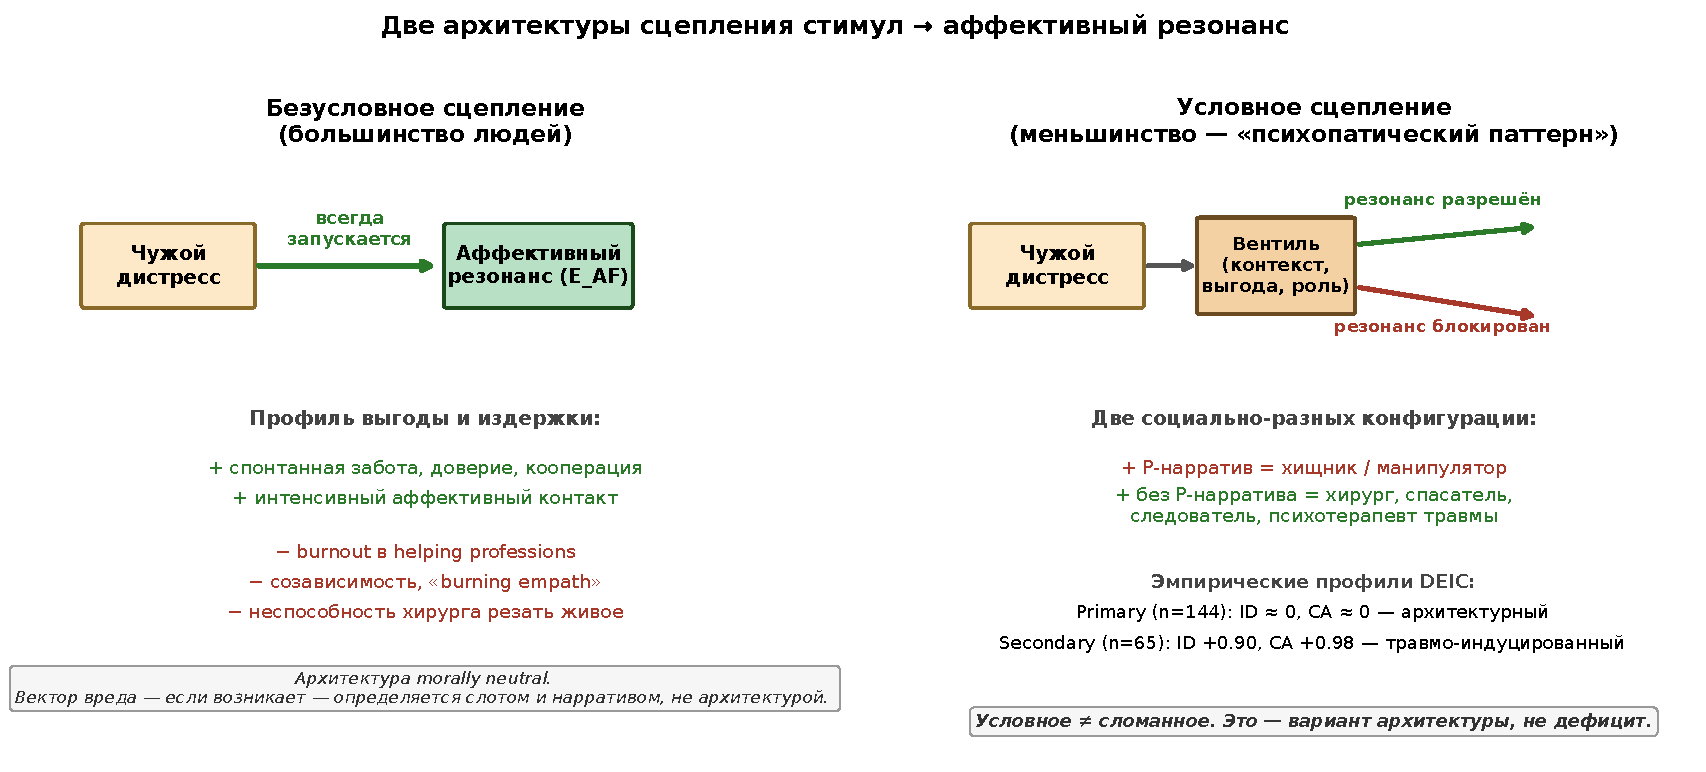
\includegraphics[width=0.95\linewidth]{figures/fig12_conditional_coupling.pdf}
\caption[Безусловное vs условное аффективное сцепление]{Архитектура сцепления \EAF{}, не дефицит. Слева: \emph{безусловное} сцепление --- аффективный резонанс запускается автоматически, почти непроизвольно, независимо от контекста и моральной оценки (базовый паттерн большинства популяции). Справа: \emph{условное} сцепление --- тот же резонанс доступен, но пропускается через контекст-зависимый gate; комбинации этой архитектуры с P-нарративом определяют социальное применение. Эмпирические профили первичной ($n = 144$; ID $\approx 0$, CA $\approx 0$) и вторичной ($n = 65$; ID $=+0.90$, CA $=+0.98$) клеток показаны как две этиологические траектории в условную архитектуру.}
\label{fig:conditional_coupling}
\end{figure} Параллели в других функциональных системах помогают удерживать рамку без нормативного сноса: люди различаются по condition-sensitivity болевой реакции, по вегетативной реактивности, по дефолтному уровню arousal. Ни одна из этих вариаций не называется поломкой по умолчанию --- каждая оценивается в конкретном контексте применения.

Условное сцепление имеет важное двойное использование, которое обычно вытесняется из клинической рамки. В социальных ролях, требующих работы внутри ситуаций страдания \emph{без} автоматического аффективного entrainment, условная архитектура --- не только совместима, но и функционально необходима. Хирург, который во время операции способен оставаться когнитивно точным при работе с живой плотью и кровью пациента. Спасательный врач, который эффективен в катастрофе именно потому, что его аффективный резонанс не парализует его действий. Следователь, работающий с показаниями жертв сексуального насилия. Психотерапевт травмы, выдерживающий многолетний поток клиентских состояний без выгорания. Каждая из этих ролей требует \emph{условного} доступа к аффективному резонансу --- способности включить и выключить резонансную сцепку сознательно. Безусловная архитектура в этих ролях даёт высокую burnout-vulnerability; условная --- устойчивость. В популяционном масштабе эта вариация обслуживает функции, которые иначе общество не могло бы заполнить.

Вредной эта архитектура становится только в сочетании с \textbf{P-нарративом} --- устойчивым моральным утверждением «мне это разрешено», которое разворачивает условную сцепку в сторону преднамеренного использования других без моральной обязанности. Именно поэтому \DEIC{} моделирует P \emph{отдельно} от \EAF{}: аффективная архитектура сама по себе морально нейтральна, а моральный нарратив --- ортогональный слой, определяющий её социальное применение. Условная сцепка без P-нарратива --- хирург; условная сцепка с P-нарративом --- хищник. Безусловная сцепка с P-нарративом --- маловероятная комбинация, которая в данных встречается редко; безусловная сцепка без P-нарратива --- базовый эмпатический паттерн большинства популяции, с его собственными уязвимостями.

В наших данных эта двухслойная логика хорошо видна в трёх эмпирических результатах. Первый --- \textbf{параллельная медиация CA $\to$ \{ID, P, M\} $\to$ \EAF{}} на единой модели (§\ref{sec:results}.4.1): путь CA $\to$ P по сути пуст ($a$-коэффициент $+0.015$, indirect effect 95\% CI $[-0.086, +0.060]$ включает ноль), в то время как путь через ID несёт $\sim 173\%$ тотального эффекта CA на \EAF{}. На уровне популяции P и CA статистически ортогональны. Это значит, что P-нарратив --- \emph{не} адаптивное следствие детской истории, а архитектурно независимый слой. Вторичный (hi-P-hi-CA) паттерн --- не «P через CA», а co-occurrence двух независимых осей в подгруппе людей. Первичный (hi-P-lo-CA) паттерн соответственно не является «психопатией без травмы в детстве», он вообще не принадлежит к той же этиологической линии, что CA-опосредованные конструкты.

Результат параллельной медиации требует честной реконсиляции с unified SEM (§\ref{sec:results}.4.2), где все пути --- параллельные медиаторы, A main-effect на \EAF{}, и модерация A на обеих стадиях ID-канала --- оцениваются одновременно. В этой более полной спецификации $a$-путь CA$\to$ID остаётся устойчивым ($+0.345$), CA$\to$P по-прежнему пуст ($+0.011$, NS), но $b$-путь ID$\to$\EAF{} коллапсирует до $-0.012$ (NS) при включении P в то же уравнение, тогда как P$\to$\EAF{} доминирует на уровне $-0.726$. Индекс модерации \IMM{}, значимый в более узкой спецификации §\ref{sec:results}.4 ($-0.00197$, CI не включает ноль), также коллапсирует до $+0.0001$ (NS), когда в той же модели P и A присутствуют как предикторы \EAF{}. Это не опровержение §\ref{sec:results}.4 и не артефакт переподгонки --- это ре-композиция дисперсии. В популяционном масштабе основная объяснительная сила \EAF{} концентрируется в P-канале (нарратив «разрешено мне») и в A-main-effect (witnessing как самостоятельный позитивный предиктор \EAF{}, $b = +0.393$), а не в изолированной ID$\times$A-модерации. На клиническом case-level каскад CA $\to$ ID $\to$ снижение \EAF{} остаётся содержательно значим --- $a$-путь реален, ID как медиатор травматического опыта в индивидуальной динамике присутствует; однако когда мы смотрим на общую выборку, прямой негативный предиктор аффективной эмпатии --- не остаточный ID, а активный P-нарратив и (в обратную сторону) активное witnessing-присутствие.

Это уточнение важно, потому что оно меняет клинико-теоретическую формулировку без потери основного содержания. Мы не утверждаем, что ID-канал отсутствует. Мы утверждаем: на уровне всей популяции ID-канал и P-канал имеют значительную общую дисперсию в предсказании \EAF{}, и в unified-модели основной вес несёт P (с его моральной подписью) и A (с его witnessing-слоем). Этот результат усиливает, а не ослабляет тезис §\ref{subsec:architecture} о двухслойной архитектуре: архитектурный уровень (условная/безусловная сцепка) и нарративный уровень (P-разрешение) работают \emph{независимо} от детской истории --- и их комбинация определяет социальное применение эмпатии куда сильнее, чем остаточный диссонанс ID сам по себе. ID --- важный индикатор того, \emph{что происходит} внутри травмированной психики; P --- решающий предиктор того, \emph{во что эта архитектура разворачивается} на поведенческом выходе.

Второй --- разделение первичного и вторичного паттернов. Через rule-based $2\times 2$ топологическую классификацию мы выделяем \textbf{первичный паттерн} ($n = 144$): условная сцепка без травматической истории, с выраженным P-нарративом, без внутреннего конфликта (ID $\approx 0$, CA $\approx 0$). Это конфигурация, стабильная во времени, не требующая травматического источника --- архитектурная вариация, на которую P-нарратив «надстраивается» как самостоятельная моральная структура \citep[в терминах][эмпирически --- в подобных пропорциях у \citealp{lilienfeld1990, patrick2010}]{karpman1941}. \textbf{Вторичный паттерн} ($n = 65$): условная сцепка с травматической историей (CA $= +0.98$), с активным внутренним конфликтом (ID $= +0.90$), с высоким Masking ($+0.63$). Это конфигурация, в которой условный режим сцепления функционально \emph{вынужден} защитной системой: автоматическое аффективное entrainment было бы разрушительно, и психика выстроила условное сцепление как адаптацию. P-нарратив здесь обычно остаётся активным, но структурно отличается --- он защищает остатки self, а не открывает доступ к хищничеству.

Третий результат --- распределение A-фактора (внимания) между группами и его взаимодействие с архитектурой. Первичный паттерн имеет умеренный A без особых корреляций с ID. Вторичный паттерн имеет низкий A ($-0.55$) --- его условная сцепка работает \emph{без} наблюдающего отношения, что делает её болезненной для самого носителя. Это прямо указывает на разные клинические точки входа: первичный паттерн не имеет «раны», которую можно лечить, и работа с ним --- структурно-социальная и нарративная (ограничение P-нарратива через внешние рамки, если это уместно); вторичный паттерн имеет «рану» в виде сохранного ID, и A-work переводит условное сцепление в интегрированный режим --- тот же профиль, что у интегрированного выжившего из §\ref{subsec:integrated_survivor}, но пришедший из другой истории.

Это не воспроизведение \emph{таксона} по \citet{hare2003} и не утверждение, что первичный и вторичный --- разные биологические виды. Мы утверждаем более скромное: архитектура условного сцепления в популяции существует как стабильная вариация, этиологически она достигается как минимум двумя путями (без травмы --- первичный; через травму как адаптация --- вторичный), и клиническая интерпретация «психопатия» смешивает эти пути, потому что на поведенческом уровне они выглядят похоже. Различить их можно только через измерение ID и CA. Без этого различия терапевтические стратегии систематически ошибаются: применение травма-ориентированных методик к первичному паттерну попадает в пустоту; применение поведенческих ограничительных методик к вторичному --- игнорирует его внутренний конфликт и потенциальный ресурс.

Размер вторичной подгруппы ($n = 65$) не позволяет надёжно оценивать величины эффектов; это ограничение требует клинической выборки для подтверждения. Но направление различения устойчиво воспроизводится в латентной топологии и не является артефактом одного индекса.

\paragraph{Возрастная инвариантность и критическое окно формирования архитектуры.} Анализ возрастной стратификации даёт один из наиболее клинически содержательных результатов программы: структурные связи между переменными --- центральный канал CA$\to$ID$\to$\EAF{}, ортогональность CA$\perp$P, ассоциации A с \EAF{} --- инвариантны в диапазоне возрастов 14--45 лет. Полная инвариантность в этом диапазоне значит, что архитектура, измеренная в наших данных, после \emph{раннего детства} структурно стабильна. Она может меняться в интенсивности (ID может ослабляться в результате терапии, A может расти в результате практики), но не в своей топологии: каналы, по которым проходит ущерб, и узлы, в которых он компенсируется, --- те же в 14 лет, те же в 45. Это указывает на то, что \textbf{критическое окно формирования архитектуры закрывается до 14 лет, и почти наверняка существенно раньше}. Нейродевелопментальная литература \citep{schore2001, perry2002, siegel2012} устойчиво указывает на первые 3--5 лет жизни как на период, в котором формируются базовые паттерны аффективной регуляции и attachment-архитектуры; наш результат совместим с этой датировкой и не противоречит ей. Практическое следствие --- структурная переформулировка prevention: если архитектура устанавливается до возраста, в котором типичный клиент попадает к клиницисту или в систему mental healthcare, то \emph{вся взрослая терапевтическая работа} --- это работа с уже сложившейся структурой, а не её первичное формирование. Рычаг первичной профилактики находится на уровне родительско-детского поля в первые годы жизни --- в поддержке mentalization-capacity родителей, в институтах раннего вмешательства, в dyadic parent-infant интервенциях \citep{powell2013}. В координатах \DEIC{} это не риторический призыв, а прямое операциональное следствие: ни одна из наших интервенционных гипотез (somatic work, MDMA-PT, psychedelic-assisted therapy, A-training) \emph{не создаёт} новую архитектуру у взрослого клиента; они все перестраивают существующую. Создание происходит до того, как клиент оказывается в состоянии обратиться за помощью.

Эта переформулировка --- архитектура вместо дефицита --- имеет последствия за пределами клиники. В уголовно-правовой системе, где психопатия часто трактуется как сочетание моральной и функциональной неисправности, разделение архитектуры (нейтральной) и P-нарратива (морально значимого) разводит то, что требует коррекции, от того, что не подлежит коррекции в принципе (архитектуру). В организационной психологии разделение позволяет видеть, что некоторые роли нуждаются в условной архитектуре и что её «лечение» противоречит функции. В публичной коммуникации --- позволяет перестать говорить о психопатах как о «сломанных людях» и перейти к разговору о комбинации способностей и нарративов, который социум может регулировать через внешние структуры, а не через попытку переделать внутреннюю архитектуру.

\subsection{Позиционирование: слон, а не мастер-карта}
\label{subsec:positioning}

Мы сознательно выбираем позиционирование, которое отличается от большинства интегративных психологических проектов. \DEIC{} не претендует быть «первым единым фреймворком эмпатии», «разрешением дискуссии между психоанализом и нейронаукой», «интеграцией всех традиций». Мы выбираем более узкую и более защитимую позицию: \DEIC{} --- это \emph{компрессия}, а не \emph{сложение}. Разные традиции (психоаналитическая, теория привязанности, когнитивная нейронаука эмпатии, зеркально-нейронная литература, клиническая традиция психопатии от Cleckley к Hare, контемплативные традиции witnessing) действительно касаются одного и того же предмета разными способами, и каждое касание --- настоящее. Наш вклад в том, что мы измерили шесть различимых функций в \emph{одной} выборке, показали их устойчивые структурные отношения и тем самым сделали видимыми \emph{суставы} между тем, что эти традиции описывают по отдельности.

Мы специально не занимаем позицию, которую \citet{wilber1995, wilber2000} занимал по отношению к традициям. Уилбер утверждал, что существует \emph{супер-карта} (AQAL: четыре сектора $\times$ уровни $\times$ линии $\times$ состояния $\times$ типы), на которой каждая традиция занимает своё иерархически определённое место. Это онтологическая претензия: карта первична, традиции вторичны, и каждая видит лишь фрагмент того целого, которое видит мета-теоретик. В нашей работе четыре реальных отличия от этой позиции важны и будут соблюдены как дисциплина, а не как стилистика.

Во-первых, уровень претензии. Уилбер строит онтологию --- мета-метафизическое утверждение о том, как устроена реальность. \DEIC{} строит measurement model --- психометрическую модель шести функций на конкретной выборке. Первое неопровержимо по конструкции; второе должно воспроизводиться в новых выборках, и если не воспроизводится, оно опровергнуто.

Во-вторых, иерархия координат. В AQAL уровни иерархичны и нормативны: integral $>$ pluralistic $>$ rational $>$ mythic $>$ magical $>$ archaic. В \DEIC{} шесть координат не иерархичны. Нет предустановленной позиции, что «высокое A лучше» или «низкое P лучше»; есть эмпирические корреляции с исходами, но это следствия данных, а не нормативные оценки. «Интегрированный выживший» --- один профиль среди многих, а не вершина.

В-третьих, отношение к традициям. Уилбер ассимилирует: каждая традиция получает место на \emph{его} карте, и её внутренняя структура переинтерпретируется через AQAL. \DEIC{} не размещает традиции. Мы говорим: «измеренный нами конструкт X коррелирует с тем, что в традиции A называют \textit{sākṣī}, в традиции B --- \textit{rigpa}, в традиции C --- самовоспоминание». Эти описания в своих системах автономны. Мы не встраиваем системы в \DEIC{}; мы показываем, где психометрическая координата \emph{нашей} модели коррелирует с тем, что описывают они.

В-четвёртых, скромность относительно непонятого. Уилбер объясняет всё, включая внутренние противоречия --- они ассимилируются как «более низкий уровень смотрит на более высокий». \DEIC{} имеет эксплицитный список того, что он не объясняет (см. §\ref{sec:limitations}, §\ref{sec:future}): временной каркас, механизм переключения между ID и P, механизм терапевтической силы A, индивидуальные различия в A-trainability, developmental branching в $2\times 2$, эволюционно-экологическая подложка, рефлексивность наблюдателя. Это не дефект, это граница.

Короткая формула, которая будет повторяться в этом разделе несколько раз: Уилбер --- «я вижу целое; традиции видят части моей карты; вы сейчас на уровне X»; \DEIC{} --- «я вижу шесть измеримых функций. Некоторые традиции описывают одну из них глубже, чем мы. Координатный каркас --- не метафизика, а статистика; его можно и нужно опровергать».

\subsection{Дисциплина анти-Уилбер: гигиена языка}
\label{subsec:discipline}

Позиция из §\ref{subsec:positioning} реализуется через набор дисциплинарных правил, которые должны выполняться в каждом абзаце. Первое правило --- каждое утверждение о конструкте сопровождается фальсификатором. Если мы пишем «A модерирует канал CA$\to$ID$\to$\EAF{}», мы обязаны добавить: «если в pre-registered replication \IMM{} 95\% CI включает ноль, это утверждение опровергнуто». Этим мы отличаем \DEIC{} от систем, которые объясняют всё (и тем самым не объясняют ничего).

Второе --- запрет иерархии между факторами. Мы не пишем «A --- зрелость», «интегрированный выживший --- высшая точка», «witnessing --- более развитый уровень». Мы пишем «эмпирически связано с [конкретный результат]». Это может показаться педантизмом, но именно в этой точке большинство мета-теоретических проектов сходит с рельсов: нормативный язык встраивается незаметно и закрывает дорогу эмпирической проверке.

Третье --- не ассимилировать традиции, но и не держать их на символической дистанции. Мы не пишем «Дзен --- это про A». Мы пишем «Дзен описывает похожий конструкт в своей системе; корреляция с нашей моделью --- такая-то». Если мы не можем сделать вторую часть утверждения, мы не делаем и первую. При этом мы \emph{делаем} вторую часть --- и делаем её развёрнуто, когда традиция даёт операбельное различение, которое в психометрической литературе пока не воспроизведено. Культурологические референты (адвайта, дзогчен, Четвёртый путь, non-dual современность, Маккенна) в \DEIC{} --- не декоративное оформление и не проявление академической смелости в ущерб строгости; они источники гипотез, которые мы либо формулируем как фальсифицируемые, либо оставляем без упоминания. Байесовский приор при расхождении наших данных с контемплативной традицией --- «мы ещё не измерили то, что они различают», а не «они ошибались».

Четвёртое --- measurement model $\neq$ онтологические претензии. Мы не пишем «\DEIC{} описывает психику». Мы пишем «\DEIC{} --- психометрическая модель шести функций на $N = 1426$ русскоязычной онлайн-выборке». Это ограничение претензии, которое защищает нас от превращения в мета-теорию.

Пятое --- лексическая дисциплина. \emph{Extends, operationalizes, is consistent with, replicates within our framework, provides psychometric coordinates for} --- разрешено. \emph{Unifies, completes, first to integrate, resolves, supersedes, subsumes} --- запрещено. Выбор глагола в ключевом утверждении программы --- это выбор между серьёзной работой и мета-теоретической претенциозностью.

Шестое --- обязательная секция «что \DEIC{} не объясняет» видимого размера, не в сноске (см. §\ref{sec:limitations}--\ref{sec:future}).

Седьмое --- reflexivity clause: в методологической статье программы будет эксплицитный раздел о том, что наблюдатель (исследователь) со своим уровнем A влияет на то, что он способен измерить у наблюдаемого. Это структурное эпистемологическое признание, а не мистическая ремарка.

\subsection{Фальсифицируемость как структурный уровень}
\label{subsec:falsifiers}

Генеративный характер модели важнее её описательного характера. Все предсказания, сформулированные в предыдущих подразделах Обсуждения, --- двухстадийная A-модерация канала CA$\to$ID$\to$\EAF{}, коллапс $b$-пути ID$\to$\EAF{} в unified SEM, ортогональность CA$\perp$P на популяционном уровне, различимость первичной и вторичной психопатии, \EAF{}-эффект в интегрированно-выжившей клетке, hyper-instrumentation P$\to$\Ecog{} и прочие --- вынесены в отдельный структурный раздел (§\ref{sec:falsification}) в форме claim/falsifier-пар с явно указанными требованиями к тесту и последствиями опровержения. Тот раздел не является расширенным комментарием к Обсуждению; он формулирует, \emph{при каких именно наблюдениях} утверждения этой статьи следует считать ложными. Для чтения Обсуждения это означает: все утверждения в findings-регистре («данные показывают», «модель даёт») имеют научный статус ровно в той мере, в какой в §\ref{sec:falsification} сформулирован их фальсификатор. Этот раздел --- не приложение к статье, а условие того, что статья принадлежит к эмпирическому жанру, а не к риторическому.

\subsection{Отношение к существующим теориям}
\label{subsec:relation_to_theories}

\DEIC{} совместим с большинством основных линий эмпатии и психопатии, но в ряде точек не совпадает с доминирующими интерпретациями. Мы не заявляем, что эти линии ошибочны целиком; мы указываем точки, в которых наша модель расходится с ними.

\citet{baroncohen2011} EQ как диспозиционная черта --- в нашей модели \EAF{} --- state, регулируемый A; trait-модель пропускает ядро механизма. «Psychopaths lack cognitive empathy» --- популярное упрощение; наши partial correlations показывают обратное: $r$(P, \Ecog{}) $= +0.32$ после partialling. Когнитивная эмпатия у психопатов часто \emph{повышена}; именно это обеспечивает возможность «хищничества», как описано у \citet{blair2013} и \citet{baroncohen2011} под рубрикой hyper-instrumentation. Hare'овский таксон-взгляд на психопатию --- мы не находим categorical kinds в наших данных. Dimensional-модель с двумя ортогональными этиологиями точнее описывает топологию наших результатов. \citet{newman2003} response modulation theory как универсальное объяснение психопатии --- у наших P-паттернов когнитивное внимание сохранно; witnessing-аффективная сцепка работает в \emph{условном}, а не безусловном режиме. Ответно-модуляционное объяснение фиксирует часть этого механизма --- избирательность внимания, --- но не отделяет архитектурный слой (условное сцепление, морально нейтральное) от нарративного (P-разрешение).

Classic attachment determinism \citep{bowlby1969} в упрощённом прочтении: CA $\to$ dysfunction линейно. Наши данные показывают модерацию через A. Детерминизм ложен; компенсация эмпирически реальна. \citet{vaillant1977} иерархия зрелых/незрелых защит --- мы не находим, что защиты per se патологичны. ID без A даёт дисфункцию; ID с A --- функциональную компенсацию. Моральная рамка «зрелая защита лучше незрелой» оказывается менее информативной, чем рамка «защита плюс witnessing».

NICE/APA CBT-first для всех расстройств настроения \citep{nice2022, apa2019}. \DEIC{} прямо предсказывает, что у high-ID / low-A клиентов CBT попадёт в сопротивление или даст поверхностное улучшение без изменения базового механизма. Self-reported psychiatric dx count как severity measure --- наши данные показывают, что ID блокирует help-seeking, поэтому dx\_count \emph{недооценивает} самых тяжёлых случаев. FFMQ \citep{baer2006} как операционализация mindfulness --- наш A-CFA эмпирически демонстрирует, что метакогнитивные айтемы смешивают attention-to-internal-states с witnessing. Мы поддерживаем критику \citet{vandam2018}. \citet{wilber1995, wilber2000} AQAL --- мы прямо не воспроизводим иерархически-стадиальные модели развития сознания в наших данных. Мы не находим stages; мы находим дистрибутивные неиерархичные координаты.

\subsection{Расширение ACE: «не помню» как часть конструкта, а не пропуcк}
\label{subsec:ace_extension}

Стандартная операционализация adverse childhood experiences, идущая от \citet{felitti1998} и закреплённая в CDC/Kaiser-линии и практически во всём производном корпусе, допускает у респондента два легитимных ответа на каждый ACE-айтем: «да» (событие было) и «нет» (не было); всё остальное --- «не помню», «не уверен», отказ --- трактуется как missing data, исключается или импутируется. ACE-айтемы при этом спрашивают не об эмоциональной интерпретации детского опыта, а о \emph{фактах}: был ли родитель в заключении, употребляли ли в семье вещества, происходило ли домашнее насилие, умер ли родитель, развелись ли родители. На фактологический вопрос ответ «не помню» в популяционной перспективе имеет ровно две содержательные интерпретации, и \emph{ни одна из них не сводится к статистической missingness}. Первая: респонденту не рассказывали --- что само по себе является маркером семейного паттерна замалчивания вокруг высокоадверсивной среды (семьи, в которых систематически обсуждают умершего родителя или эпизод насилия, производят других респондентов, а не тех, кто отвечает «не помню»). Вторая: респондент диссоциировал --- что является прямой поведенческой манифестацией того самого защитного механизма D, который ID-латент измеряет на другом конце инструмента. Обе интерпретации ACE-релевантны; обе эмпирически противоположны трактовке «не помню» как missing. Стандартная кодировка в таком случае \emph{исключает из анализа ровно тот подконтингент, на котором ACE-сигнал должен быть наиболее силён}. Это не мелкая кодировочная деталь, а структурный недо-учёт в стандартной методологии ACE, наследованный всем корпусом.

DEIC-конструкт предлагает расширение: ответ «не помню» на ACE-айтеме следует трактовать как \emph{позитивный сигнал адверсивно-релевантной семейной или когнитивной конфигурации} --- либо семейного замалчивания, либо диссоциативного encoding-gap, --- и кодировать численно наравне с «да». Тогда ACE перестаёт быть одномерным счётчиком событий и становится двухслойным: явный счёт подтверждённых событий плюс счёт ответов «не помню» как отдельная ACE-dissociation подшкала.

Эмпирическая валидация расширения получена на текущей выборке через полный re-fit 6-факторной oblique CFA, в которой канонический код «не помню»~$=$~NaN заменён на «не помню»~$=$~1. Из 1470 респондентов 667 (45.4\%) использовали «не помню» хотя бы один раз на 10 ACE-айтемах; 294 (20\%) --- дважды и более. Под расширенной кодировкой N проходит фильтр $\le$10\% missing уже 1468 (против канонических 1426), средний ACE-счёт сдвигается с 3.43 до 4.18, MLR-robust CFA сохраняет приемлемый фит (CFI~$=$~0.960, TLI~$=$~0.949, RMSEA~$=$~0.062 против канонических 0.950, 0.936, 0.068; df~$=$~120 в обоих случаях). Латентные корреляции в 6-факторной oblique модели сдвигаются в направлении, согласующемся с DEIC-гипотезой: $r(\text{CA}, \text{ID})$ растёт с $+0.668$ до $+0.712$, $r(\text{CA}, \EAF{})$ усиливается по модулю с $-0.129$ до $-0.205$ ($+59\%$), $r(\text{CA}, M)$ растёт с $+0.195$ до $+0.267$, тогда как $r(\text{CA}, P)$ остаётся слабой (рост с $+0.015$ до $+0.122$ --- всё равно в пределах «слабой» связи), сохраняя архитектурную орто\-гональность P к детской адверсии.

Параллельная медиация CA~$\to\{$ID, $P$, $M\}\to\EAF{}$ на латентных scores split-B под канонической и расширенной кодировкой (5000 bootstrap-draw) даёт согласованно усиленную картину. Суммарный эффект $c$(CA~$\to$~\EAF{}) усиливается по модулю с $-0.129$ до $-0.205$. Косвенный эффект через ID --- канонический канал «защита убивает эмпатию» --- сохраняет структуру: $-0.223$ [$-0.267, -0.181$] под канонической кодировкой, $-0.236$ [$-0.282, -0.192$] под расширенной; CI в обоих случаях не пересекает ноль. Косвенный эффект через P \emph{становится статистически отличимым от нуля} именно при расширении: канонический $-0.014$ [$-0.086, +0.060$] (нз), расширенный $-0.140$ [$-0.234, -0.048$] (стат.~значимый). Это не переопределяет архитектурную орто\-гональность P к CA как популяционный факт, но указывает, что часть P-канала была инструментально недо-замечена именно там, где у респондента включена диссоциативная кодировка детства. Прямой эффект $c'$ (CA~$\to$~\EAF{} при контроле ID, P, M) остаётся положительным при обеих кодировках ($+0.073$ канонический, $+0.048$ расширенный), то есть headline sign-flip главного mediation-вывода --- «травма бьёт по эмпатии через защиту, а не напрямую» --- устойчив к способу кодировки «не помню». Ни один из 95\%-ных bootstrap-интервалов для исходных статзначимых индиректов не пересекает ноль под расширенной кодировкой, то есть сдвиги численно различимы, а не шумовые.

Операциональное следствие для волны 2: ACE-айтемы сохраняют трёхвариантный формат «да / нет / не помню», но «не помню» кодируется как позитивный сигнал; счётчик таких ответов по всем 10 айтемам строится как самостоятельная ACE-dissociation подшкала. Психометрическое предсказание: при $n \ge 300$ эта подшкала должна давать McDonald's $\omega \ge 0.7$ и положительно коррелировать с ID-латентом ($r \ge 0.30$ при латентном оценивании); при её контроле связь «явного» ACE-счёта с ID должна ослабевать, что даёт формальный тест валидности подшкалы как отдельного канала. Концептуальное следствие шире. Мы не утверждаем обобщение \emph{эффект-сайзов} на весь корпус ACE-литературы --- для этого нужен мета-аналитический re-фит; мы указываем на \emph{структурную} проблему в кодировочной логике, наследованной всем корпусом \citep{felitti1998}. Там, где эта логика одинакова, одинаков и направленный смыслостроительный сдвиг: любой self-report сенситивной информации ранних лет жизни --- сексуального анамнеза, substance-history, семейных секретов --- где «не помню» является легитимным и социально-приемлемым ответом, требует явного моделирования этого ответа как construct-relevant signal, а не механического сведения к missing. См. §\ref{sec:future} о дизайне wave-2 и §\ref{sec:limitations} о границах текущей оценки.

\subsection{Декларативно-поведенческая асимметрия (DI) как сигнал архитектурной фрагментации}
\label{subsec:di_asymmetry}

Пилотная композитная версия инструмента (DEIC-DRAFT, август 2025) была построена на принципе парных формулировок: каждый содержательный айтем существовал в декларативном регистре (абстрактная self-description: «я эмпатичный человек», «я манипулирую другими», «я подавляю свои эмоции») и поведенческом регистре (конкретная узкоокнская поведенческая репортация: «вчера я остановился и действительно выслушал», «на прошлой неделе я скрыл от партнёра важную деталь ради своей выгоды», «сегодня утром я сдержался от того, чтобы показать раздражение»). Сводный индекс $DI = \overline{\text{decl}} - \overline{\text{beh}}$ по всем айтемам в пилоте показал статистически значимый популяционный сдвиг ($p < 0.001$, $d \approx 0.43$) с ведущим вкладом шкалы AIS (декларативно 5.04 vs поведенчески 3.35). На этом основании в пилотном отчёте DI был описан как самостоятельный индикатор social desirability. Ниже мы показываем, что это описание было частично неверным: популяционный сдвиг воспроизводится, но по шкалам он разнонаправлен, и то, что DI на самом деле измеряет --- не однородное искажение самопрезентации, а \emph{архитектурный разрыв между абстрактным self-schema и эпизодической поведенческой памятью}.

На основной выборке ($N{=}1470$) декларативно-поведенческий разрыв посчитан по восьми шкалам с достаточным балансом парных айтемов (ADI, CA, D, EC, Empathy, Psychopathy, Suppression, Masking; 38 декларативных против 40 поведенческих). Парные $t$-тесты значимы на всех восьми шкалах, но распределение $d$ по модулю и направлению существенно различается. Положительные DI (декларация превышает поведение) --- E ($d{=}{+}0.44$), EC ($d{=}{+}0.45$), ADI ($d{=}{+}0.20$), CA ($d{=}{+}0.19$). Отрицательные DI (поведение превышает декларацию) --- P ($d{=}{-}1.05$; крупнейший эффект на выборке), MS ($d{=}{-}0.30$), S ($d{=}{-}0.10$), D ($d{=}{-}0.09$). Суммарный сырой DI оказывается слабо отрицательным ($d{=}{-}0.11$) --- знак усреднения разнонаправленных шкал. Если же DI выровнять в prosocial-направлении (для стигматизированных шкал знак перевернуть, так чтобы $+$ всегда означало «я декларативно прохожу как более положительная версия себя, чем показывает моё поведение»), сдвиг становится однородно положительным: $d_{aligned}{=}{+}0.29$, 95\%CI $[{+}0.14, {+}0.20]$. Пилотное наблюдение, таким образом, воспроизводится, но как \emph{совокупный результат двух разных механизмов}, а не однородный social-desirability bias.

Разведение этих механизмов --- главный содержательный результат этого раздела. Для стигматизированных шкал с явным self-incriminating содержанием (P, MS, S, D) поведенческие айтемы узкой фокусировки («на этой неделе я...») собирают больше признаний, чем декларативные trait-описания, --- то, что респондент не готов присвоить как черту, он готов признать как эпизод. Наиболее ярко это проявляется на P: пара $P_4$ («я манипулирую людьми, чтобы получить желаемое») --- $P_{\text{new\_3}}$ (конкретное поведенческое описание эксплуатационной ситуации за прошедший период) даёт средний разрыв $-2.66$ балла по 7-балльной шкале ($d{=}{-}0.98$), то есть respondent систематически отрицает trait-схему психопатии, но отчётливо опознаёт конкретные её проявления в собственном поведенческом архиве. Это воспроизводит давнее клиническое наблюдение о расщеплении между trait-идентификацией и эпизодическим поведенческим self-report при психопатическом нарративе \citep{hare2003, lilienfeld1990} на операциональном уровне. Для desirable-валентных шкал (E и, с оговоркой, EC) направление противоположно: trait-schema широка, поведенческий эпизод узок --- respondent держит развитое самопредставление об эмпатичности, которое опирается на широкую историю, в то время как конкретный narrow-window beh-айтем («сегодня утром я \ldots») попадает или не попадает в конкретный поведенческий эпизод. Для shared-adversity шкал (ADI, CA) положительный разрыв указывает на противоположный паттерн: trait-уровень отчасти overstates внутреннюю историю, которой конкретный поведенческий эпизод в повседневности не подтверждает --- возможное методологическое следствие того, что ADI- и CA-декларативные айтемы опрашивают глобальный аффективный self-concept, не привязанный к недавнему коду.

То, что DI не сводится к social desirability, подтверждается связями с латентной архитектурой. $DI_{overall}$ (сырой, ненаправленный) коррелирует с ID как $r{=}{+}0.590$, с CA как $r{=}{+}0.580$ и с A как $r{=}{-}0.517$; с клинической диагностической переменной ($\text{dx\_free\_text\_any}$) --- $r{=}{+}0.017$ (нз, $p{=}0.66$). Иначе говоря, величина декларативно-поведенческого разрыва отслеживает \emph{внутреннюю фрагментацию между слоем trait-self-schema и слоем episodic-behavior-recall}, и эта фрагментация маркирована тем же архитектурным латентом (ID), который во всей остальной работе фиксируется как защитный контур. $A$ как witnessing-функция сужает разрыв. Клинический статус в этом не участвует, что структурно последовательно с $\S\ref{subsec:architecture}$ и $\S\ref{subsec:free_will}$: DI --- архитектурная, а не диагностическая метрика. $DI_{aligned}$ (развёрнутый в prosocial-направлении) даёт зеркальную картину: $r(DI_{aligned}, A){=}{+}0.658$, $r(DI_{aligned}, \EAF{}){=}{+}0.550$, $r(DI_{aligned}, ID){=}{-}0.645$, $r(DI_{aligned}, P){=}{-}0.362$. При медианном расщеплении по $A$ контраст $DI_{overall}$ между low-A и high-A даёт $d{=}0.90$ (терцильный --- $d{=}1.22$), то есть $A$-поле полностью перестраивает направление и величину разрыва.

Отдельный результат касается $piz$ --- интегральной метрики, реализованной в инструменте для отслеживания фасадной работы (masking+Lie; $\S\ref{subsec:integral_metrics}$). $piz$ и DI структурно различны и эмпирически различны. $r(piz, DI_{overall}){=}{+}0.198$ (small positive), $r(piz, DI_{aligned}){=}{-}0.274$ --- то есть $piz$ и $DI_{aligned}$ даже расходятся по знаку (более высокое маскирование $\Rightarrow$ \emph{меньший}, а не больший prosocial-сдвиг декларации над поведением). На отдельных шкалах $r(piz, DI_{P\_scale}){=}{+}0.359$: более высокое маскирование связано с более выраженным $\textit{beh}>\textit{decl}$ разрывом на P-шкале (высокая facade-работа усиливает именно ту ассиметрию, при которой trait-отрицание идёт рука об руку с поведенческим признанием). В сумме: $piz$ измеряет самопрезентационное давление, $DI$ измеряет структурную фрагментацию --- два разных слоя, оба операционализуемы.

Для инструментальной инфраструктуры это означает, что $DI$ имеет смысл фиксировать рядом с $piz$ как шестую \texttt{extended\_metric} в \texttt{psychometrics.json} (с per-scale и overall-aligned версиями). Для теоретической рамки --- что пилотное наблюдение восстанавливается, но в содержательно уточнённом статусе: оно даёт операциональную psychometric-сетку для давнего психоаналитического различения между «идеальным Я» как trait-schema и «действующим Я» как поведенческим архивом \citep{freud1917, winnicott1965}, при этом разрыв между ними --- не дефект измерения, а содержательный маркер архитектуры. Методологическое следствие для wave-2: любая психометрическая шкала, претендующая на диагностическую функцию в $ID$/$P$/$E$-доменах, должна включать парные декларативные и поведенческие формулировки, потому что именно их разрыв, а не любая из двух формулировок по отдельности, даёт доступ к архитектурному слою.

\subsection{\DEIC{} и теория сознания: граница, на которой мы работаем}
\label{subsec:consciousness}

\DEIC{} не предлагает теорию сознания. Hard problem \citep{chalmers1995} --- граница, через которую психометрия не проходит и не должна делать вид, что прошла. Мы измеряем функции \emph{внутри} сознания (внимание, диссонанс, эмпатия); мы не утверждаем ничего о природе субъективного опыта как такового, и это ограничение серьёзное, а не риторическое.

Но из того, что граница реальна, не следует, что от неё нужно держаться на дистанции. Наоборот: именно вблизи этой границы происходит самый содержательный интерфейс эмпирической психометрии с contemplative studies. A --- психометрический след того, что в различных традициях выделяется как структурно иной слой сознания: \textit{sākṣī} в адвайте, \textit{rigpa} в дзогчене, «самовоспоминание» у Гурджиева, non-dual awareness в современной non-dual литературе. Мы не объясняем, что такое свидетель. Мы показываем, что witnessing измеримо, функционально, и что его действие на канал CA$\to$ID$\to$\EAF{} воспроизводимо в узкой спецификации. Это делает A точкой, в которой психометрия \emph{соприкасается} с разделом сознания, который обычно считается вне-функциональным, --- не ассимилируя его и не заявляя о его природе, но и не обходя его стороной.

Самый резкий диалог этого типа --- с \citet{mckenna2002, mckenna2004, mckenna2013}. В большинстве западных репрезентаций contemplative traditions пробуждение описывается аддитивно: больше осознанности, больше принятия, больше присутствия. McKenna это переворачивает. Его тезис --- \emph{spiritual autolysis}: пробуждение есть разрушительный процесс, растворение иллюзорных структур, а не наращивание новых способностей. Больше внимания не приносит утешения; оно раскрывает сконструированность собственных состояний и мира, и это раскрытие не приятно. Обычный человек уклоняется от него, потому что там нет утешительной рамки.

В рамке \DEIC{} тезис McKenna формулируется как прямое longitudinal-предсказание. У людей, проходящих intensive retreats с глубокой witnessing-практикой, A растёт. Если McKenna прав, на коротком промежутке времени ID \emph{возрастает} --- раскрытие сконструированности даёт временную дестабилизацию identity, то есть именно ту сигнатуру, которую в нашей cross-sectional модели мы читаем как диссонанс. Траектория после этого разветвляется: либо регрессия (защиты возвращаются, A падает обратно, дестабилизация закрывается обычной структурой), либо интеграция (принятие сконструированности, профиль, топологически соответствующий integrated survivor из §\ref{subsec:integrated_survivor}, но пришедший не через детскую травму, а через добровольный практический путь). Это не предсказание «верный ли McKenna»; это операционализация его тезиса в виде, который может быть опровергнут longitudinal-данными на retreat-когортах.

Это и есть наше положение относительно теории сознания. Не заменять её, не претендовать на её территорию --- но и не делать из её существования предлог, чтобы избегать контакта. На границе работать можно и нужно: делать конкретные психометрические предсказания в тех точках, где contemplative traditions удерживают операбельные различения, которые эмпирическая психология пока только начинает уловить.

\subsection{Клинические импликации}
\label{subsec:clinical}

Модель имеет несколько конкретных клинических следствий, которые мы формулируем как \emph{предложения для тестирования}, а не как рекомендации к немедленному внедрению.

\paragraph{Работа с A до работы с содержанием.} У клиентов с высоким ID и низким A прямая когнитивная интервенция часто попадает в сопротивление или даёт поверхностное улучшение. Наша модель предсказывает, что последовательность «A-work $\to$ content-work» будет эффективнее, чем «content-work без предварительного A». Это формализует то, что somatic experiencing \citep{levine2015}, sensorimotor psychotherapy \citep{ogden2006}, IFS \citep{schwartz1995}, mentalization-based therapy \citep{fonagy2008} и ряд психодинамических подходов делают интуитивно. Pre-registered RCT с baseline A и ID как модератором эффекта лечения --- прямой тест.

\paragraph{Различение первичного и вторичного паттернов в клинической оценке.} Без измерения ID и CA два паттерна выглядят одинаково, но требуют разных стратегий. Первичный --- условная архитектура без «раны»: клиническая работа с архитектурой как таковой бесполезна и даже может быть неуместной (в функциональных социальных слотах эта архитектура даёт устойчивость); работа с P-нарративом через внешние рамки --- адекватна тогда, когда нарратив разворачивается в хищническую сторону. Вторичный --- работа с травмой и расширение A, с целью перевода сохранного ID в интегрированный режим.

\paragraph{A-training как центральный компонент долгосрочной работы.} Наша модель предсказывает, что non-dual mindfulness практика будет давать более сильный эффект на \EAF{}-восстановление, чем behavioral-mindfulness в стиле MBSR. Это формулирует head-to-head testable сравнение.

\paragraph{Burning empath как feed-forward риск.} Профиль CA + hi \EAF{} + lo A должен предсказывать burnout в helping professions.

\paragraph{Substance use как phenotype, не причина.} В подгруппе blocked-sober-high-P наблюдается тот же профиль P/D/ACE, что и у активных пользователей веществ. Это указывает, что substance --- \emph{выход} блокировки, а не её источник. A-training в работе с addictive behaviors должен давать устойчивый эффект там, где abstinence-based программы рецидивируют.

\paragraph{Терапевт с низким A не видит ID-активации клиента.} Это имеет прямое клиническое следствие: supervision и self-work клинициста --- не nice-to-have, а структурное условие возможности видеть то, что у клиента происходит.

\subsection{Свобода воли как градиент внимания}
\label{subsec:free_will}

Одно из наиболее концептуально тяжёлых следствий \DEIC{} --- реформулировка проблемы свободы воли. Мы не претендуем её решить. Мы утверждаем, что в её классическом бинарном виде --- «свободна ли воля?» --- она поставлена в неверной зернистости и потому не имеет ответа. В зернистости, которую даёт наша модель, она распадается на конкретный эмпирический вопрос: \emph{какова величина A в конкретной ситуации у конкретного агента?}

В DEIC-координатах поведение можно читать как результат взаимодействия двух слоёв: автоматической D/P/E-конфигурации (что запускается как ответ на стимул без участия наблюдающего отношения) и A (зазор между запуском и действием, в котором возможно иное распределение внимания, иное соотнесение, иная реакция). Low-A-агент в конкретный момент функционально детерминирован своей конфигурацией: стимул активирует канал, канал разворачивает автоматическое поведение, наблюдение отсутствует. High-A-агент в том же моменте имеет \emph{измеримый зазор} между активацией и действием, внутри которого возможна иная траектория. Это не метафизическое различие, а эмпирическая переменная --- та же, которую фиксирует наша A-модерация в узкой спецификации: при высоком A канал CA$\to$ID$\to$\EAF{} меняет знак именно потому, что A вклинивается между привычным триггером и его привычным исходом.

Философы, спрашивавшие о свободе воли, подходили к одному и тому же градиенту с разных сторон. Августиново «раб воли» и его описание \textit{liberum arbitrium captivatum} есть описание low-A состояния, в котором желание непрерывно разворачивается в действие без зазора. Кант и его примат практического разума --- описание функции, которая появляется при высокой A: \emph{Maxime} как осознаваемый принцип поведения, а не импульс. \citet{libet1985} с его ранней готовностной потенциалом и критики его интерпретации \citep[см.][]{frith2008} указывают на то, что волевой акт действительно иногда запаздывает относительно мозговой активности, но \emph{veto-функция} остаётся --- это и есть A, удерживающая зазор. \citet{frankl1946} --- «между стимулом и ответом есть пространство; в этом пространстве наша сила выбирать наш ответ» --- прямое описание A-модерации в клиническом языке. Буддистская \textit{vīmaṃsā} (исследующее внимание) и \textit{yoniso manasikāra} (обдуманное внимание) описывают практики, наращивающие A как условие этической возможности; адвайтическое различение \textit{vṛtti} (движения ума) и \textit{sākṣī} (наблюдающего) --- ту же самую структурную асимметрию. Гурджиевское «человек-машина» есть описание low-A-режима, а «самовоспоминание» --- операциональный протокол подъёма A. Когда эти линии сходятся на том, что обычный человек большую часть времени действует из автоматизма, а моменты свободы связаны с особым качеством внимания, они сходятся не случайно --- они описывают одно и то же измеримое явление в разных языках.

Из этого прочтения следует серия предсказаний. Во-первых, восприятие агенсом собственного волевого акта как «свободного» должно коррелировать с его моментальным A, а не с его trait-уровнем самоэффективности или с нарративом самодетерминации. \citet{westgate2019}-type парадигмы meaning-in-action могут быть переформатированы как A-assays. Во-вторых, интервенции, повышающие A (non-dual mindfulness, somatic work, psychedelic integration), должны давать измеримый рост переменных, которые обычно связываются с self-determination: внутренняя мотивация, моральная консистентность, способность отказаться от краткосрочного вознаграждения в пользу долгосрочной ценности. В-третьих, популяции с систематически подавленным A (см. §\ref{subsec:political}) должны демонстрировать систематически меньшую функциональную свободу выбора --- не как моральный дефект, а как прямое следствие разрушения операциональной инфраструктуры свободы.

Этическое следствие этого прочтения --- не отмена ответственности, а её структурная перекалибровка. Вопрос «был ли он свободен в тот момент?» получает эмпирический ответ: какова была его A-конфигурация в момент действия, какова была дисперсия его A во времени, какова траектория её развития. Ответственность сохраняется, но распределяется иначе: за конкретное действие в low-A-моменте --- меньшая по интенсивности, чем за долгосрочную траекторию заботы о собственной A-инфраструктуре. Это совпадает с интуицией, которую клинический здравый смысл и ряд правовых систем уже используют de facto (смягчающие обстоятельства, concept diminished capacity, forensic-оценка состояния на момент деяния), но делает её операциональной. Прощение, которое в большинстве традиций формулируется этически («прости им, ибо не ведают, что творят»), становится эпистемологически корректной атрибуцией: в low-A-моменте агент не ведал, потому что инфраструктура ведания не была развёрнута.

Мы подчёркиваем, что это не отменяет различия между действиями, произведёнными из low-A-автоматизма, и действиями, произведёнными с A-поддержкой из выраженного P-нарратива. Первые --- структурно несвободны и, как правило, стандартная терапевтическая и образовательная работа --- адекватный ответ. Вторые --- архитектурно другие: высокое A, удерживающее P-нарратив «мне это разрешено», не есть отсутствие свободы, это выбор из высокого A в пользу нарушения. Социальный и правовой ответ на эти два класса действий должен быть структурно разным, и \DEIC{} предлагает координатную сетку, в которой такое различение можно делать операционально, а не импрессионистически.

\subsection{Политика, медиа, внимание: DEIC на социальном масштабе}
\label{subsec:political}

Выходы \DEIC{} за пределы индивидуальной клиники требуют отдельного разговора. Мы формулируем их как \emph{дискуссионные тезисы для будущих программ исследования}, а не как готовые политические рекомендации. Связь между architecturой индивидуальной психики и социальными паттернами не прямая, и всякое утверждение о социальном масштабе на основе N$=1426$ русскоязычной онлайн-выборки --- это гипотеза, а не установленный факт. Однако именно потому, что \DEIC{} содержит явные операциональные координаты, эти гипотезы можно сформулировать так, чтобы их можно было проверять.

\paragraph{Политическая демагогия как P$\times$low-A-рынок.} Политический стиль, который в литературе описывается как популистский/демагогический, в DEIC-языке имеет чёткую сигнатуру на стороне лидера: высокое P (моральный нарратив разрешённости --- «я их ведущий, мне можно решать за них»), умеренная условная \EAF{} (достаточная для ритуального performance, не парализующая действие), и --- \emph{существенно} --- высокая \Ecog{} (инструментальное понимание аудитории). Это не ad hominem атрибуция конкретным политикам --- это описание структурной ниши, которая в популяции с низким A оказывается социально адаптивной и селективно предпочитаемой. \citet{westen2007, haidt2012} показывают, что аудитории голосуют не столько рационально, сколько через моральные и идентификационные контуры; наша рамка уточняет: аудитории с низкой A-инфраструктурой выбирают не идеи, а моральные нарративы, которые совпадают с их собственным нерефлексивным self-concept. Предсказание: электоральная поддержка P-стильной демагогии должна предсказываться не по социоэкономическим маркерам per se, а по общему A-уровню аудитории в момент выборов.

\paragraph{Attention economy как структурно психотогенная среда.} Если A --- структурное условие интеграции и, следовательно, условие возможности устойчивой психики (см. §\ref{subsec:integrated_survivor}), то среда, систематически разрушающая A, действует как психотогенный агент на популяционном уровне. Современные engagement-оптимизированные медиа-системы --- структурно такая среда. Механизм трёхслойный: (а) фрагментация A через micro-interruption (уведомления, непрерывный feed, swipe-интерфейсы), (б) выведение P-контента на поверхность как engagement-максимума (возмущение, моральное негодование, identity-сигналинг), (в) доставка утешительного D-контента (echo-chamber подтверждение имеющейся защитной конфигурации). В сумме --- одновременное падение A, рост P-паттернирования в массовой коммуникации, стабилизация D. Это прочтение наблюдаемой «эпидемии тревоги/СДВГ/поляризации» как не эпидемии отдельных расстройств, а как единой структурной деградации DEIC-конфигурации в популяции. Конкретные testable предсказания: (i) интенсивность использования engagement-оптимизированных платформ предсказывает снижение A в 6--12-месячных лонгитюдах; (ii) подростковые когорты с ранним exposure к алгоритмически-курируемому feed имеют измеримо иную DEIC-топологию, чем когорты с тем же ACE-load, но без раннего exposure; (iii) эксперименты с attention-protective дизайном (edit-mode, pause-интерфейсы, slow-feed) должны давать измеримый прирост A при прочих равных.

\paragraph{Демократия как A-dependent институт.} Мы формулируем это осторожно, потому что утверждение такого масштаба требует корректного масштаба данных. Тем не менее: если демократическое участие структурно предполагает способность удерживать сложный моральный и когнитивный объект (политическое решение) достаточно долго для его обдумывания --- то есть предполагает A, --- то демократия в среде систематического A-разрушения не может поддерживать собственную функцию. Это не аргумент против демократии; это аргумент о том, что демократия исторически держалась на attention-protective инфраструктуре (церковь, образование в его старом виде, медленные медиа, коммунальные институты), которую секуляризация и коммерциализация не заменили эквивалентом. Результат --- регрессия политики в populism, поляризация, высокая susceptibility к P-стилю. Практическое следствие: инвестиции в attention-protective институты --- образовательная реформа, контемплативная компонента в общей педагогике, regulation engagement-оптимизации как public health issue --- структурно необходимы для поддержания демократической функции. Это тезис, который в нашей выборке прямо проверить нельзя, но который логически вытекает из обнаруженной нами A-модерации индивидуального функционирования.

\paragraph{Культы, авторитарные движения, сектантская политика.} Рамка позволяет прочесть динамику культов и авторитарных движений в единой логике: лидер несёт доминирующий P-нарратив избранности или исключительности; последователи приносят D и низкий A --- поиск внешней структуры, которая обойдётся без необходимости самостоятельного наблюдения; культ даёт кажущуюся интеграцию через внешнюю структуру вместо внутреннего A-развития. Это прочтение делает разборную работу с ex-cult members и ex-radicalised лицами не просто когнитивной дерадикализацией, а восстановлением A-инфраструктуры, которую движение подавляло. Эмпирически testable: DEIC-профили людей, выходящих из культовых/авторитарных движений, должны характеризоваться low A и профилем D, сохранившемся в замороженном виде; длительная терапевтическая работа должна сопровождаться ростом A и высвобождением удерживавшегося D-содержания.

\paragraph{Коллективная D и transitional justice.} Пост-геноцидные, пост-тоталитарные, пост-колониальные общества несут коллективный аналог индивидуальной D-конфигурации: системно подавленное, аффективно неинтегрированное отношение к собственной исторической реальности, передающееся трансгенерационно \citep{yehuda2015, meaney2001}. \citet{herman1992} в своей формулировке complex trauma указывает на коллективный слой; наша рамка делает измеримым предположение, что transitional justice (truth commissions, memorial practices, public historical reckoning) работает именно как коллективная D-work --- поэтому он эффективен там, где выделяет пространство для аффективной интеграции, и неэффективен там, где сводится к процедурной юридической форме. Русскоязычная выборка, на которой валидирована наша модель, несёт повышенный baseline CA/ID, плотно связанный с двумя войнами двадцатого века, репрессиями и девяностыми; мы предполагаем (и ждём cross-cultural replication), что это не культурный шум выборки, а измеримая коллективная D-конфигурация, отражённая в индивидуальной психике.

\paragraph{Религии, секулярное замещение, коллективная A-инфраструктура.} Мы описываем это как дискуссионный тезис, стремясь удержаться равно далёким от религиозной апологетики и от секулярной дисмиссии. Эмпирически: основные религиозные традиции исторически содержали три функциональных компонента, систематически работавших с DEIC-конфигурацией --- A-тренинг (молитва, медитация, ritual examen), D-aperture (исповедь, коллективный плач, ритуальный траур), P-границу (заповеди, испытание совести). Секулярные современные замены (терапия, wellness-индустрия, философия практической жизни) пытаются воспроизводить часть этих функций в индивидуальной добровольной форме, но без institutional-уровня continuity и без коллективной инфраструктуры. Прогноз: секулярные общества должны \emph{заново построить} эквивалент коллективной DEIC-калибровочной инфраструктуры или принимать эпидемиологические издержки. Это не аргумент в пользу возвращения религии в её исторических формах --- это аргумент в пользу того, что функция, которую эти формы выполняли, не исчезла оттого, что исчезли формы.

\subsection{Эволюционный масштаб: интеграция как биологическое требование}
\label{subsec:evolutionary}

Наиболее широкий вывод, который мы готовы сформулировать, --- чтобы читатель увидел масштаб, на котором \DEIC{} может работать, даже если он не поместится в одну эмпирическую статью. D и P как архитектуры --- древние, эволюционно подготовленные. D есть расширение freeze-response (позвоночная иммобилизация под угрозой) в эмоциональный и социальный домен. P есть производное dominance-стратегии в приматной социальной иерархии. Оба механизма были адаптивны в среде, для которой они создавались: эпизодическая острая угроза с быстрым разрешением (freeze), локальная иерархическая конкуренция с ясными правилами (dominance). Обе эти архитектуры активируются сейчас в контекстах, для которых они не создавались --- хроническое экономическое давление, непрерывный media-мониторинг, сложная символическая социальная экология, --- и оттого переходят из адаптации в хроническую мал-адаптацию. Это evolutionary mismatch в его структурно-психологическом изводе \citep[в духе][]{lieberman2013, sapolsky2017}.

Из этой рамки вытекает одно из самых серьёзных следствий \DEIC{}, которое мы готовы отстаивать как гипотезу-тезис для последующих эмпирических программ. \emph{Мы --- вероятно, первое поколение в истории вида, для которого интегрированная взрослая жизнь есть биологическое требование, а не роскошь.} Эволюция не проектировала механизм взрослой интеграции, потому что до недавних историко-демографических сдвигов большинство людей умирали или структурно были вовлечены в жизнь клана/племени/ритуальной общности до того, как нерезолвированные D/P могли разрушить индивидуальную жизнь; короткая жизнь, ритуальная инфраструктура, встроенные формы коллективного A (см. §\ref{subsec:political}) выполняли работу интеграции за индивида. Современный 80-летний человек, живущий в нуклеарной семье, с 40-летним продуктивным трудом, с экспозицией к хронической информационной стимуляции, с атомизированной социальной сетью, --- живёт с защитным аппаратом, рассчитанным на временное использование, в среде, которая требует постоянной интеграции того, что эволюция вообще не готовила к интеграции.

Следствие, которое мы формулируем как тезис, требующий проверки долгосрочными population-level данными: \emph{созерцательная и терапевтическая работа --- не улучшения базовой функции, а \textbf{предварительное условие выживаемости} в наших текущих биологических и экологических координатах}. В этом смысле массовая потребность в терапии, растущий спрос на meditation и psychedelics, популяционный интерес к соматическим практикам --- не культурная мода, а биологический сигнал о том, что конфигурация нервной системы, сложившаяся для среды двадцати-тысячелетней давности, недостаточна для среды, в которой она сейчас живёт, и требует дополнительной индивидуальной intervening работы для функционирования.

В эмпирической своей части этот тезис порождает конкретные предсказания: (i) population-level индикаторы A (переносимость скуки, способность удерживать единый объект, distress tolerance) должны монотонно падать с ростом уровня urban engagement-density; (ii) incidence клинических D-dominant расстройств должна расти не пропорционально ACE per se, а пропорционально \emph{разрыву} между ACE-загрузкой и доступностью integration-инфраструктуры; (iii) когорты со структурным доступом к integration-инфраструктуре (длительная терапия, ретрит-культура, contemplative education) должны показывать измеримо иную траекторию mental health на 20--40-летнем лонгитюде, чем демографически сравнимые когорты без такого доступа.

\subsection{Структурная недоразмерность современной помощи}
\label{subsec:undersizing}

Наиболее клинически серьёзное следствие \DEIC{}-рамки, которое требует отдельного обсуждения: современная система mental healthcare \emph{структурно} не того масштаба, на котором заявлена её задача. Это утверждение резкое, и мы понимаем его резкость. Мы формулируем его как дискуссионный тезис и попытаемся защитить эмпирически, а не риторически.

Классическая травма-терапия в её современном медицинском формате --- 20 сессий CBT, SSRI-поддержка, структурированные психообразовательные модули --- эффективна для post-formation adjustment disorder: для взрослой психики с сложившейся до травмы структурой, для которой травма есть разрыв непрерывности, требующий переработки. Для \emph{personality-formative early D}, когда D-конфигурация сложилась в первые 3--5 лет жизни и стала основанием последующего развития --- когнитивного стиля, attachment-паттерна, desire-архитектуры, identity, --- такая терапия структурно недоразмерна.

Причина конкретна. Для раннего формирующего D \emph{не существует пред-травматического self как референта восстановления}. Вся структура сложилась как адаптация к небезопасности; восстановление означает не возврат к чему-то, что было разрушено, а реорганизацию структуры, построенной на D-основании. В терминах, которые будут узнаваемы для контемплативных линий --- буддистская \textit{saṃsāra} в её этическом аспекте, исихастское «совлечение ветхого человека», суфийское \textit{fanā}, --- это процесс пересборки, а не починки. Такой масштаб работы не помещается в протокольную рамку с предсказуемым числом сессий и стандартизованным исходом.

Что мы знаем о методах адекватного масштаба. Традиционные формы: длительные монашеские ретриты (3-year-3-month в тибетской традиции, multi-year vipassana, исихастский подвиг, suf\=i \textit{halva}) требовали institutional continuity, которая в современных секулярных обществах почти исчезла. Современные клинические аналоги: длительный интенсивный психоанализ (4--5 сессий в неделю в течение многих лет в Kernberg-style работе), therapeutic communities в Soteria-традиции \citep{mosher1999} --- почти утерянная институция; multi-year ayahuasca-циклы в традиционных контекстах и их современные терапевтические трансляции \citep[см.][в ceremonial framework]{nielson2018}; ibogaine и 5-MeO-DMT-ассистированные протоколы с extended integration \citep[в Мексике/Нидерландах, см. обзор][]{brown2019}; long-term IFS/somatic work (многолетняя работа с постепенной реструктуризацией без катастрофического распада).

Чего \emph{нет} в современной mental healthcare: секулярного, страховкой-покрываемого, массово-доступного пути адекватного масштаба для раннего формирующего D. Это не «неэффективность», это структурное несоответствие инструмента задаче. \DEIC{} эту диагностику делает операциональной через измерение baseline D + A + CA: инструмент позволяет \emph{pre-treatment} стратифицировать клиентов на тех, для кого symptom-management интервенция адекватна (adjustment-level D без раннего формирования), и тех, для кого необходимы интервенции структурного уровня (formation-level D при высоком CA-loading и low A-инфраструктуре).

Это не призыв отказаться от symptom-management --- он нужен и полезен в своей нише. Это призыв перестать использовать symptom-management-инструмент как universal standard-of-care для структурно иных задач. Клиническое следствие: ещё один аргумент в пользу того, что DEIC-профиль на baseline должен становиться стандартом стратификации в research и, в перспективе, в клинической practice. Пациенту с раннесформированным D, направленному на 20-сессионный CBT, мы сейчас предлагаем палллиативный protocol, продаваемый под именем definitive treatment; DEIC-стратификация позволяет честно сказать: для этой структуры нужна другая интервенция, которая сейчас либо не существует в доступной форме, либо требует приватного ресурса, либо расположена за пределами медицинского фрейма (длительная somatic work, psychedelic-assisted therapy в её развёрнутой форме, long-term group/therapeutic community). Перестройка системы под этот масштаб --- отдельная программа, выходящая за рамки академической психологии, но логически вытекающая из наших данных.

\subsection{Фармакология, нозология, диагностика: \DEIC{} как переорганизующая координата}
\label{subsec:pharmacology_nosology}

Если \DEIC{} --- корректная операциональная координата, то под эту координату можно перепрочитать несколько смежных областей. Мы этого разворачивания не завершаем в данной статье; мы показываем, как оно может выглядеть, чтобы читатель мог видеть масштаб, в котором рамка работает --- и в котором её предстоит проверять.

\paragraph{Фармакология как DEIC-модификация.} Если каждый психоактивный класс характеризуется тем, какую компоненту D/P/A-конфигурации он модифицирует и в каком направлении, то клинические исходы должны предсказываться не диагностической меткой, а DEIC-профилем на baseline. Рабочие гипотезы для последующих эмпирических программ: \textbf{SSRI} снижают D-salience, не растворяют D-структуру --- отсюда характерный profile «функционален, но отключён» на длительном приёме и аддитивность с терапией только при наличии в терапии реальной A/D-работы. \textbf{Бензодиазепины} стабилизируют D через подавление thaw-сигналов --- длительный приём препятствует интеграции, поддерживая материал, который иначе мобилизовал бы её. \textbf{Антипсихотики} ослабляют и P-нарратив (через лобную модуляцию), и крайний D (через дофаминовое приглушение) --- объясняет их кросс-диагностическую функциональность и цену в виде общей A-flatness. \textbf{Классические психоделики} (psilocybin, LSD, DMT, mescaline) --- единственный известный класс, напрямую растворяющий D через DMN-дезорганизацию; дифференциальное следствие, которое мы формулируем как прямое testable predictions: psilocybin-assisted therapy должна давать большой эффект на D-dominated профили (депрессия, PTSD, устойчивая диссоциация) и малый или обратный эффект на P-dominated профили (нарциссическая патология, антисоциальность), потому что mystical experience без D-substrate может реактивно валидировать P-нарратив. \textbf{MDMA} --- уникальная конфигурация «E-ceiling + D-dissolve + A-preserve», структурно совместимая с D-dominant PTSD; при P-dominant структуре эффективность должна снижаться, и это различение должно проявиться в post-approval клинической данных. \textbf{Кетамин} --- парадокс «диссоциация для растворения диссоциации»: короткое окно высокой пластичности, на котором застрявший D размораживается при адекватной integration-инфраструктуре. \textbf{Стимуляторы} --- A-bandwidth без модификации D или P: при neurodevelopmental ADHD (low ACE) --- чистый выигрыш; при trauma-origin ADHD (high ACE + D-фрагментация внимания) --- выигрыш в продуктивности, но не в благополучии. \textbf{Опиаты} --- homecoming-класс для safety-deficit D: возвращают телу регуляцию, которую не обеспечило раннее окружение, что объясняет высокую корреляцию opioid addiction с ACE+D baseline и делает наивные воля-ориентированные подходы к opioid dependency структурно ошибочными. Каждое из этих предсказаний --- отдельная тест-программа; вместе они задают вопрос, можно ли реорганизовать клиническую психофармакологию вокруг DEIC-профилей как стратификационной переменной, а не вокруг DSM-меток.

\paragraph{Травмо-терапии декодированы через единый DEIC-механизм.} EMDR работает как принудительная вставка A в D-запечатанную память через билатеральную стимуляцию; отсюда сильный эффект на D-trauma и малый эффект на P-нарратив. Somatic experiencing \citep{levine2015} --- титрованный D-thaw через прямой выход на freeze-release в нервной системе, обходя когнитивный доступ; работает именно потому, что D формировался дословесно. IFS \citep{schwartz1995} --- экстернализация частей и быстрый A-upgrade через именование; работает и на D-профилях (части, удерживающие freeze), и на P-профилях (части, удерживающие разрешающий нарратив). CBT --- A через когнитивный слой; силён на P-нарратив, слаб на D (нельзя challenge недоступному чувству). Долгий психоанализ --- медленный A через нарратив, с переносом как живым каналом доступа к D-материалу. Групповая терапия --- четырёхслойное взаимодействие: распределённое зеркало для A-bootstrap, ко-регуляция D через несколько тел одновременно, peer-конфронтация P, растворение стыда через параллельные истории \citep[см. собранные обзоры по common factors в][]{wampold2015}. Psychedelic-assisted therapy в группе --- теоретический максимум по количеству одновременно задействованных механизмов интеграции, что соответствует эмпирически нащупанному shamanic-traditional формату. Эта типология --- не утверждение об относительном превосходстве одной школы над другой, а предлагаемая координатная сетка, на которой разные школы видны как дополняющие друг друга, работающие с разными компонентами одной DEIC-конфигурации.

\paragraph{Нозологическая переорганизация.} Мы формулируем эту часть как наиболее дискуссионную. DSM в его текущей форме организует расстройства по фенотипической поверхности (симптомам); DEIC-прочтение предполагает, что большое число ко-морбидностей в DSM --- это множественные выражения одной конфигурации канала. MDD + GAD + PTSD + диссоциативные расстройства в DSM есть часто одна конфигурация «hi ACE + hi D-dissociation + hi D-suppression + moderate A» в DEIC. Не-response и рецидив предсказываются не диагнозом, а профилем. Это совместимо с trans-diagnostic движениями (HiTOP, RDoC), но парсимоничнее каждого --- работает на меньшем числе осей. Мы формулируем это как будущую тест-программу: воспроизведёт ли DEIC-профиль на baseline больший процент дисперсии клинического ответа, чем DSM-метка, в большой ретроспективной re-analysis? Если да --- нозологическая реорганизация обретает эмпирическую опору. Если нет --- рамка ограничивается более узкими применениями. Это проверяемое, falsifiable утверждение, а не мета-теоретическая претензия.

\paragraph{Self-report-based нозология имеет нижнюю границу наблюдаемости.} Это важное ограничение для всей клинико-эпидемиологической литературы: D блокирует help-seeking и смазывает self-report, поэтому dx\_count и аналогичные счётчики клинической загрузки \emph{систематически недооценивают самых тяжёлых}. Почти вся нормативная психология построена на полупрозрачной популяции --- на тех, у кого D достаточно невысок, чтобы они заполнили анкету, пришли на оценку или оказались в клинической регистрации. Это не техническая придирка к конкретным данным; это структурное свойство всей методологической инфраструктуры. \DEIC{}-рамка делает эту слепую зону явной: когда мы видим в популяции профиль с очень высоким D и очень низким A, мы предсказываем, что в этой части выборки плотно сконцентрированы люди, которые не попали бы в данные, если бы мы не делали специальных усилий. Методологическое следствие для дальнейшей работы: active recruitment того типа, который обычно рекомендуется в community psychiatry, --- не опция улучшения выборки, а структурное условие её валидности.

\subsection{Wave-2 редизайн: от диагноза к новому инструменту}
\label{subsec:wave2_design}

Большинство ограничений настоящей работы --- не фундаментальные дефекты теории, а сигналы редизайна инструмента. В этой подсекции мы сводим данные, показывающие структурные проблемы шкал wave-1, в конкретные предложения для wave-2 DEIC-Inventory. Не на уровне отдельных айтемов (это --- задача psychometric-iteration с cognitive interviewing и pilot-study), а на уровне архитектурных решений: какие шкалы остаются, какие расщепляются, какие поглощаются, какие получают новый дизайн. Эти предложения --- контракт между настоящей статьёй и будущей публикацией wave-2 инструмента: последняя сможет ссылаться сюда как на диагностическое обоснование своей структуры.

\paragraph{A: dedicated witnessing-scale, разведённая с hypervigilance.} Wave-1 использовал A как composite из метакогнитивных айтемов. Tier~5 A-CFA (§\ref{subsec:A_as_field_condition} и §\ref{sec:limitations}) показал: при попытке рефлексивной факторизации \emph{чистейшего} 17-айтемного пула нагрузки биполярны (8 положительных, 9 отрицательных), и латентный A в SEM переворачивает знаки ключевых коэффициентов. Диагноз: пул айтемов не разделяет \emph{witnessing} (нерефлексивное наблюдение-наблюдения в нондуальной традиции) от \emph{trauma hypervigilance} (болезненная гипервнимательность к внутренним состояниям, структурно \emph{усиливающая} защиту, а не ослабляющая её). Оба дают положительный self-report на «я замечаю свои внутренние состояния» --- операционально они разные. Wave-2 предложение: \textbf{(a)} \emph{два отдельных латента} --- Witnessing (W) и Hypervigilance (HV) --- с явно разведённым контентом по четырём лингвистическим традициям (\emph{satipaṭṭhāna}, \emph{sākṣī}, \emph{rigpa}, self-remembering); \textbf{(b)} ключевой дескриптор witnessing --- «наблюдение без вмешательства, без реактивности, без желания изменить содержание»; ключевой дескриптор HV --- «постоянное сканирование на опасность, тревожный мониторинг»; \textbf{(c)} differential-validity проверка: W должен положительно коррелировать с distress tolerance и с interoceptive accuracy, HV --- отрицательно с distress tolerance. Dedicated W-scale --- приоритет номер один в wave-2.

\paragraph{M: расщепить instrumental и reactive masking.} Wave-1 M имел $\omega = 0.546$ против $> 0.89$ у остальных пяти факторов, и латентная корреляция $r(M, P) = +0.82$ не даёт клинически осмысленного различения. Диагноз: M-шкала конфаундирует два феноменологически различных паттерна --- instrumental masking (осознанное управление фасадом, close to P, «как выглядеть нужным образом») и reactive masking (автоматическое социальное подстраивание под угрозу, close to ID, «как не стать заметным»). Wave-2 предложение: \textbf{(a)} расщепить на M\textsubscript{inst} и M\textsubscript{react}; \textbf{(b)} M\textsubscript{inst} должен иметь высокую корреляцию с P и низкую с ID, M\textsubscript{react} наоборот; \textbf{(c)} валидация через item wording с явным различением намерения и автоматизма.

\paragraph{ID umbrella: сохранить концептуальный центр, восстановить SUP как отдельный латент, доработать DIS и AIS.} Bifactor-анализ (§\ref{subsec:id_bifactor}) показал гетерогенность поглощения пяти wave-1 защит общим ID-латентом: IDS (0.66) и FLA (0.86) почти полностью описываются общим ID, DIS (0.54) и AIS (0.53) держат около половины subscale-specific дисперсии, SUP --- только 31\%. Wave-2 предложение: \textbf{(a)} \textbf{ID} остаётся как umbrella-латент (Internal Dissonance, наследник IDS), с IDS-айтемами и FLA-айтемами как чистыми индикаторами; \textbf{(b)} \textbf{SUP} восстанавливается как \emph{отдельный латент подавления} --- эго-синтонное сознательное inhibition, не часть пассивного блокирования; SUP должен положительно предсказывать executive control и negative affect regulation в короткой перспективе, но \emph{не} предсказывать trait-ID; \textbf{(c)} для DIS и AIS айтемы переработаны с контентным форсированием различий: DIS-айтемы акцентируют эго-дистонный автоматизм расщепления, AIS-айтемы --- «содержание есть, чувство отрезано» (классический интеллектуализатор); ожидается, что после переработки bifactor будет иметь чистую структуру с общим ID и отдельными чистыми DIS/AIS-specific-факторами.

\paragraph{E\textsubscript{AF} и E\textsubscript{cog}: разведение на item-level, не post-hoc.} Расщепление эмпатии на аффективную и когнитивную было сделано в настоящей работе post-hoc, в ответ на P$\leftrightarrow$E парадокс. Диагноз: wave-1 шкала E смешивала оба компонента в одних айтемах, что алгебраически гарантировало confounding. Wave-2 предложение: \textbf{(a)} отдельные item-sets для E\textsubscript{AF} (эмоциональное заражение, аффективное резонирование, соматические маркеры чужого состояния) и E\textsubscript{cog} (перспективизм, mentalizing, прочтение интенции) --- ровно один фактор на айтем в primary-scale; \textbf{(b)} минимальный контентный overlap между двумя subscale; \textbf{(c)} pre-registered prediction: bifactor с общим E и двумя specific-factors должен дать ECV\textsubscript{global} $< 0.5$ (то есть компоненты разделимы), а P на латентном уровне должен давать $r(\text{P}, \text{E\textsubscript{cog}}) > 0$ и $r(\text{P}, \text{E\textsubscript{AF}}) < 0$.

\paragraph{P: расширение контентного покрытия и разведение моральной под-шкалы.} Wave-1 P оперировал относительно узким single-dimensional пулом, близким к Psychopathic Personality Inventory (Lilienfeld \& Andrews, 1996) и Dark Triad (Paulhus \& Williams, 2002). Диагноз: публикуемые findings (hyper-instrumentation, orthogonality to CA, primary/secondary topology) получены на сравнительно узком итеме; разветвление на первичный/вторичный паттерны, предсказанное теорией, не подкреплено контентно дифференцированным дизайном; моральная составляющая P («разрешено мне», которая отличает архитектурную психопатию от профессиональной диссоциации) не разведена от архитектурной (switching resonance). Wave-2 предложение: \textbf{(a)} расширить контентное покрытие за счёт items, специфичных для primary (coldness, callousness, \emph{low}-anxiety variant Karpman) и secondary (reactive aggression, high-anxiety, trauma-linked); \textbf{(b)} отдельная под-шкала \textbf{P\textsubscript{moral}} --- айтемы о том, что субъект считает допустимым \emph{для себя} (не про других): «для меня нормально лгать, если это работает», «мои эмоциональные правила отличаются от общепринятых»; \textbf{(c)} архитектурная P\textsubscript{arch} --- айтемы о capacity для сознательного переключения resonance: «я могу включать/выключать сочувствие в зависимости от того, с кем говорю». Предсказание: P\textsubscript{moral} и P\textsubscript{arch} должны быть различимы (latent $r \approx 0.4$--$0.6$), но обе давать positive partial с E\textsubscript{cog}.

\paragraph{CA и ACE: сохранить как единый латент, добавить под-шкалы типов травмы.} Wave-1 ACE и CA на нашей выборке взаимозаменяемы (latent $r > 0.8$), поэтому объединены в единый CA-латент. Диагноз: объединение не теряет общей дисперсии ранней реляционной истории, но сглаживает различие между типами неблагоприятного опыта (физическое насилие vs эмоциональная депривация vs нестабильность привязанности vs сексуальная травма). Wave-2 предложение: сохранить единый CA-латент как primary, но ввести четыре наблюдаемых под-индекса (CA\textsubscript{phys}, CA\textsubscript{emot}, CA\textsubscript{attach}, CA\textsubscript{sex}) для дескриптивного различения при сохранении общего латента для SEM-каналов.

\paragraph{Lie-шкала: перенести от ковариаты к активной корректирующей метрике.} Wave-1 Lie-шкала работала как ковариата social desirability; в настоящей работе она входит в формулы коррекции интегральных метрик (§\ref{subsec:integral_metrics}). Диагноз: Lie-шкала полезна, но в wave-1 использует традиционный social-desirability item-set (близко к Marlowe-Crowne и BIDR), который смешивает impression management и self-deception. Wave-2 предложение: расщепить на IM (impression management --- сознательное искажение для внешнего observer'а) и SD (self-deception --- неосознанное искажение самовосприятия); разная диагностическая функция: высокий IM при низком SD означает ответственное self-presentation, высокий SD --- активную защиту self-image'а, релевантную ID-структуре.

\paragraph{Архитектурные решения.} Три изменения в scoring-инфраструктуре для wave-2, прямо следующие из limitations \S\ref{sec:limitations}: \textbf{(1)} двухуровневое \texttt{questions.json} с \texttt{factor\_weights} (для CFA с явно прописанными cross-loadings) и \texttt{primary\_scale} (для композитного sum-scoring, один айтем $=$ один композит) --- устраняет multi-scale inflation; \textbf{(2)} публикуемая модель по умолчанию --- bifactor (общий ID плюс specific-factors), а не чистая oblique, --- чтобы исходящая структура отражала реальную гетерогенность; \textbf{(3)} A вынесен из 6-factor oblique в отдельный формативный блок, с последующей рефлексивной witnessing-scale как параллельным ref-point'ом.

Переход от wave-1 к wave-2 --- не косметическая переработка шкал, а структурная перепосадка. Настоящая статья документирует диагностические основания каждого изменения; следующая статья программы (wave-2 validation, pre-registered, на новой выборке) будет ссылаться на эту подсекцию как на свою дизайн-базу.

\subsection{Интегральные метрики: реализованные в инструменте клинические индикаторы}
\label{subsec:integral_metrics}

Инструмент DEIC-Inventory помимо шкальных баллов возвращает клиенту и клиницисту набор сводных индикаторов, вычисляемых из уже нормированных шкальных значений (шкалы нормированы в $0$--$100$; базовые переменные в формулах ниже --- это эти нормированные значения). В \texttt{psychometrics.json} эти индикаторы фиксируются в блоке \texttt{extended\_metrics} как формулы с явно перечисленными переменными и вычисляются в \texttt{calculations.ts}; здесь мы приводим их в том виде, в каком они реально используются в инструменте, а не как отдельные теоретические конструкции. Все формулы ниже --- это рабочие клинические индикаторы, не валидированные psychometric-параметры; они \emph{предложены}, а не установлены, и требуют конкурентной валидизации против существующих инструментов до того, как могут применяться для формальной диагностики.

\paragraph{R-метрика (базовая метрика эмпатического резонанса).} Определена в блоке \texttt{r\_metric} как
\[
R_{\text{metric}} \;=\; (\text{empathy} - \text{suppression} - \text{dissociation} + 50)\,(1 - \text{psychopathy}/100).
\]
Смысл: эмпатия, скорректированная на два основных канала пассивной блокировки (подавление и диссоциация), и далее умножённая на фактор $(1 - P/100)$, который подавляет итоговое значение у респондентов с высоким P-нарративом. Константа $+50$ удерживает базовую величину в положительной области при типичных уровнях защит. R-метрика --- входная переменная всех профильных правил в \texttt{psychometrics.json.profiles} (frozen, adaptive, psychopathicDeficit, modestlyBlocked и др.) и используется как ключевой индикатор клинической стратификации в инструменте.

\paragraph{$R_{+}$ (с поправкой на присутствие witnessing).} Определена в \texttt{extended\_metrics.rPlus} как R-метрика, дополнительно модулированная шкалой внимания:
\[
R_{+} \;=\; R_{\text{metric}} \cdot (\text{attention}/100).
\]
Эквивалентно: $(\text{empathy} - \text{suppression} - \text{dissociation} + 50)\,(1 - \text{psychopathy}/100)\,(\text{attention}/100)$. Клинический смысл: реализованная --- а не потенциальная --- эмпатия, то есть величина, которая согласно архитектуре \DEIC{} соответствует эмпатическому выходу, реально доступному respondent'у в повседневности, а не тому, на который он способен в принципе. Аналитическая функция витнессинга в этой метрике зеркалит главный теоретический результат §\ref{subsec:A_as_field_condition}: А работает как мультипликативный модификатор, а не аддитивный предиктор --- без witnessing-функции даже сохранная аффективная эмпатия реализуется не полностью.

\paragraph{defensiveHardness (композит аффективных защит).} Определён в \texttt{extended\_metrics.defensiveHardness} как сумма четырёх защитных субшкал:
\[
\text{defensiveHardness} \;=\; \text{suppression} + \text{dissociation} + \text{flattening} + \text{affectiveIsolation}.
\]
Смысл --- суммарная «жёсткость» аффективной регуляции, толщина защитного слоя между переживанием и поведенческим выходом. В отличие от латентного ID (который включает также IDS и другие индикаторы), defensiveHardness --- чисто аффективная композиция, прикладная для клинициста, оценивающего, насколько пациент доступен для прямой эмоциональной работы в её первоначальной фазе.

\paragraph{empathicConflict (индекс внутреннего эмпатического конфликта).} Определён в \texttt{extended\_metrics.empathicConflict} как
\[
\text{empathicConflict} \;=\; \text{internalDissonance} + \bigl[(\text{empathy} - 50) - (\text{suppression} - 50)\bigr].
\]
Конструкция фиксирует структурное несоответствие между декларированной способностью к эмпатии и активной работой её подавления. Скобочная разность $(\text{empathy} - \text{suppression})$ эмпирически представляет именно тот канал, в котором у hi-empathy-hi-suppression респондентов --- клинически классический паттерн «сохранной аффективной подкладки при активной блокировке её выражения», операционально тот же архитектурный след, который на уровне SEM проявляется как значимый $a$-путь CA$\to$ID при сохранной подлежащей \EAF{}. Индекс принимает большие значения именно там, где внутренний конфликт между способностью и её подавлением активен, а не там, где одна из двух компонент просто высока.

\paragraph{piz (индекс искажения самопрезентации).} Определён в \texttt{extended\_metrics.piz} как
\[
\text{piz} \;=\; (\text{masking} + \text{lie}) / 2.
\]
Сводный индикатор пседоискренности, совмещающий M-шкалу (маскирование: фасадная стабильность) с Lie-шкалой (social desirability в узком смысле). Функционально используется как коррекция для R и эмпатического профиля в целом: высокий piz снижает доверие к высоким эмпатическим самоотчётам, поскольку указывает на активную self-presentation-работу, которая эти отчёты могла сконструировать.

\paragraph{DI (индекс декларативно-поведенческой асимметрии).} Определён в \texttt{extended\_metrics.DI} (wave-2 дополнение) как разность средних нормированных оценок между декларативными и поведенческими айтемами внутри каждой сбалансированной шкалы, со следующим overall-aligned представлением:
\[
DI_{aligned} \;=\; \frac{1}{K}\sum_{k=1}^{K} v_k\,\bigl[\overline{decl}_k - \overline{beh}_k\bigr],
\]
где $v_k{=}{+}1$ для шкал с социально-желательной валентностью и $v_k{=}{-}1$ для стигматизированных (в текущей конфигурации --- E положительная, все остальные отрицательные). Клинический смысл --- операциональный маркер разрыва между trait-уровнем self-schema и episodic-поведенческим self-report; эмпирически $r(DI_{overall}, \text{ID}){=}{+}0.59$ и $r(DI_{overall}, A){=}{-}0.52$ (§\ref{subsec:di_asymmetry}), то есть метрика трекает архитектурную фрагментацию, а не social desirability в узком смысле. Структурно отличим от $piz$ ($r{=}{+}0.20$; на $DI_{aligned}$ знак даже переворачивается до $-0.27$) --- два разных слоя самопрезентационной инфраструктуры. В web-инструменте возвращается per-scale таблицей плюс overall-aligned числом; per-scale DI полезен для качественной интерпретации (на каких именно доменах decl-beh-разрыв открывается), overall-aligned --- для stratification и как кандидат во входные переменные будущих профильных правил.

\paragraph{Комментарий к статусу метрик.} Из шести приведённых индикаторов только R используется как критериальная переменная в профильных правилах (\texttt{profiles} в \texttt{psychometrics.json}); остальные возвращаются клиенту как сводные дескрипторы профиля и доступны клиницисту для stratification, но не закреплены как cutoff-переменные в протоколе. Композитные формулы были разработаны при проектировании инструмента (DEIC-4 meta-model --- архивная версия конструкции, предшествовавшая wave-1 validation) и реализованы в рабочем движке платформы; структурно они совместимы с шестифакторной моделью, эмпирически валидированной в настоящей работе, но само их клиническое функционирование требует отдельной проверки на клинической выборке с формализованными диагнозами и конкурентной валидизации против существующих инструментов (IRI, TSCC, TAS-20, PAS, SRP-4). До этого они --- рабочие операциональные сводки, пригодные для research-описания профилей респондентов и для внутренней feedback-функции инструмента, но не для формальной диагностической практики. Wave-2 программа включает отдельную клиническую статью, пересчитывающую эти метрики на клинически диагностированной выборке и оценивающую их ROC-характеристики и incremental validity сверх существующих composite-скор.

\subsection{К программе исследований}

Настоящая статья --- центральная эмпирическая работа будущей программы \DEIC{}. Программа включает 18 планируемых статей, распределённых по пяти слоям: эмпирический (психометрические валидации на новых выборках, longitudinal, cross-cultural, informant convergence), интегративный (связь с теорией привязанности, с психоанализом, с нейронаукой), философский (A ontology как field condition, \DEIC{} и теория сознания, reflexivity, свобода воли), прикладной (клинические импликации, публичная рамка, политическая коммуникация, образование, фармакология как DEIC-координата, структурная недоразмерность помощи), мета (методологический reflexivity, observer problem, дисциплина анти-Уилбер). Амбиция проекта распределена по программе; центральная статья узко сформулирована и скромна по тону именно потому, что защищает долгосрочную работу от преждевременной критики по стилю.

\paragraph{Fertility as evidence: разветвляемость рамки как косвенный сигнал валидности.} Мы отдаём себе отчёт, что в предыдущих разделах (§\ref{subsec:free_will}--\ref{subsec:pharmacology_nosology}) шесть координат \DEIC{} развёрнуты на темы, которые обычно находятся в разных дисциплинах: клиническая практика, политическая коммуникация, эволюционная психология, фармакология, нозология, философия свободы воли. Мы не делаем этого случайно, и мы не думаем, что это «слишком широко для психометрической работы». Мы утверждаем обратное: хорошая операциональная рамка \emph{по своей конструкции} должна объяснять разное через один механизм, и разветвляемость --- не её свобода, а её контроль. Плохо построенная рамка ведёт себя одним из двух способов --- либо не объясняет ничего (слишком узкая, не переносится за пределы собственного полигона), либо объясняет всё одинаково (слишком широкая, постмодернистская, без сигнатуры механизма). \DEIC{} вместо этого должна производить \emph{специфические дифференцированные} предсказания в каждой области применения: не «всё про D», а «этот феномен --- D-dominant, этот --- P-dominant, этот --- A-deficit, а этот --- комбинация с конкретной топологией». Если рамка эту дифференцированность удерживает в пяти разных доменах одновременно --- это слабая, но нетривиальная индукционная опора её валидности. Если в каком-то из доменов она сглаживается до «всё объясняется одной коорднатой» --- это сигнал, что рамка в этой точке не держит, и её нужно уточнять. Разветвляемость, таким образом, --- часть falsification-аппарата, а не его противоположность.

Мы открыто публикуем эту программу не как обещание, а как карту. Каждая из 18 запланированных работ сформулирована как узкая, фальсифицируемая, с ограниченной претензией. Если какие-то из них не воспроизведутся --- программа корректируется в этих точках. Если значительная часть не воспроизведётся --- программа как целое под вопросом. Это и есть единственная форма, в которой амбициозный проект психологии эмпатии и психопатии может быть серьёзным: не как завершённая теория всего, а как распределённая во времени сеть проверяемых утверждений.

\section{Фальсификационные обязательства}
\label{sec:falsification}

Эта секция вынесена как отдельный структурный уровень, а не как параграф в Обсуждении, по причине, которую мы формулируем открыто. \DEIC{} претендует на масштаб, который в академической психологии традиционно вызывает скепсис --- не потому, что масштаб сам по себе подозрителен, а потому, что широкие рамки исторически редко говорили, \emph{при каком наблюдении они признают себя ошибочными}. Мы эту границу проводим сами, заранее и на видном месте. Ниже --- список предсказаний, каждое из которых сформулировано вместе со своим фальсификатором: наблюдением, при котором это предсказание следует считать опровергнутым. Опровержение каждого отдельно означает локальное обновление рамки; опровержение определённых комбинаций, указанных в §\ref{subsec:collapse_thresholds}, означает, что \DEIC{} как каркас подлежит структурному пересмотру или отзыву.

Формально, это не обещание быть правыми. Это обязательство признавать, когда мы неправы, и обязательство --- в каких именно местах и на каких именно данных проверка будет проведена.

\subsection{Ориентация в таблице обязательств}
\label{subsec:falsification_guide}

Каждое обязательство ниже имеет четыре компонента: \textbf{(1)}~утверждение (что \DEIC{} предсказывает или постулирует), \textbf{(2)}~фальсификатор (какое наблюдение делает утверждение ложным), \textbf{(3)}~требования к тесту (какой дизайн, какой размер выборки, какая инструментальная конфигурация необходимы для того, чтобы тест имел силу), \textbf{(4)}~последствие опровержения (что именно в рамке подлежит пересмотру, а не просто ослабляется). Обязательства сгруппированы по пяти тирам: измерительные (тир~А), причинно-путевые (тир~B), топологические (тир~C), архитектурные (тир~D) и программные (тир~E).

\begin{figure}[htbp]
\centering
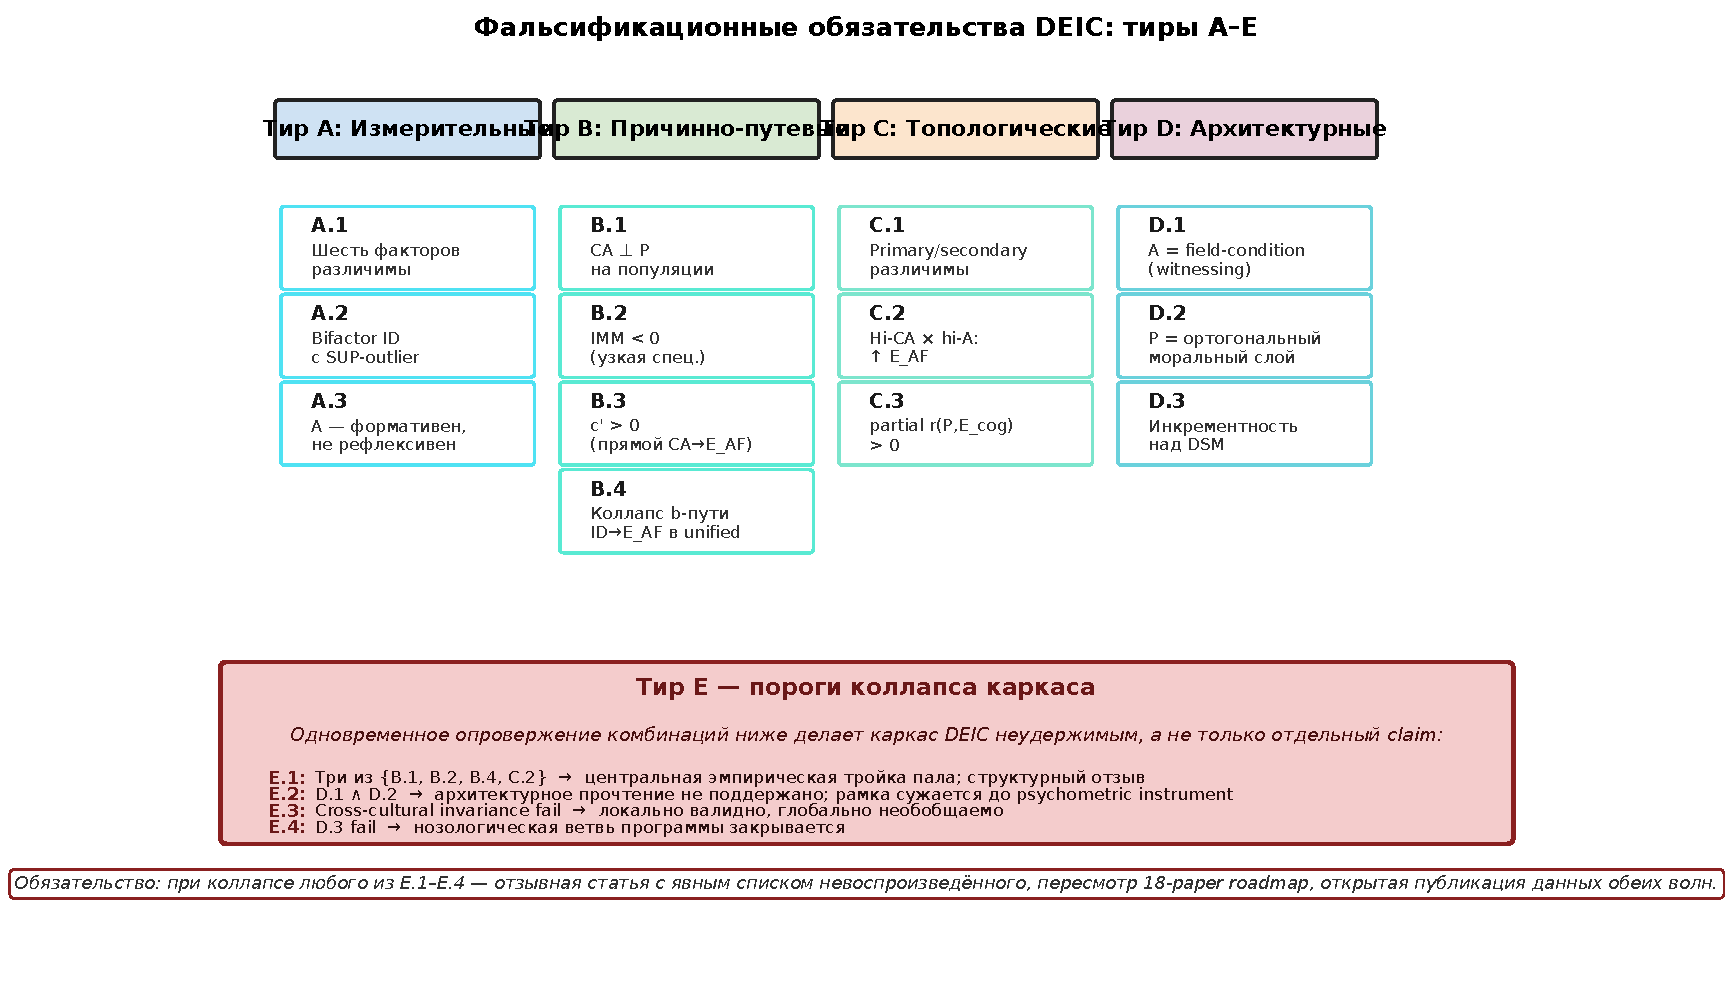
\includegraphics[width=0.95\linewidth]{figures/fig10_falsification_map.pdf}
\caption[Карта фальсификационных обязательств]{Карта фальсификационных обязательств \DEIC{}. Четыре тира локальных тестов (А --- измерение; B --- причинные пути; C --- топология; D --- архитектура) формируют верхний ряд, каждый со своими обязательствами. Нижняя красная полоса --- тир~E: пороги программного коллапса, при достижении которых каркас подлежит структурному пересмотру, а не локальному обновлению.}
\label{fig:falsification_map}
\end{figure}

Формулировки умышленно бинарны. Наука не работает в бинарных режимах --- но обязательства работают: либо мы готовы признать результат опровержением, либо мы его заранее выводим за рамки теста, и тогда это не обязательство.

\subsection{Тир А: измерительные обязательства}
\label{subsec:falsification_tier_a}

\paragraph{A.1 --- Шесть факторов различимы.}
\emph{Утверждение.} Шестифакторная oblique-CFA (ID, CA, P, M, \EAF{}, \Ecog{}) устойчиво воспроизводится на pre-registered айтемах, разведённых по дизайну.
\emph{Фальсификатор.} В волне~2 с айтемами, разведёнными по дизайну ($N \geq 1000$), либо \EAF{} и \Ecog{} сливаются в единый empathy-фактор (CFI модели с объединённой E не хуже чем с разделённой на $\Delta$CFI $\leq 0.01$), либо ID и CA неразличимы как отдельные латенты ($r_{\mathrm{lat}} > 0.90$), либо P и M неразличимы при условии инструментальной независимости.
\emph{Требования к тесту.} Pre-registered дизайн; айтемы для \EAF{} и \Ecog{} написаны по разным content-специфическим конструктам, не делят общие слова. $N \geq 1000$ для устойчивой CFA на 6 факторах.
\emph{Последствие опровержения.} Многомерная архитектура эмпатии в текущем виде не поддержана; \DEIC{} сужается до факторной структуры, которую данные держат (возможно, четырёх- или пятифакторной).

\paragraph{A.2 --- Bifactor-структура ID с SUP-как-отдельным.}
\emph{Утверждение.} ID-umbrella лучше описывается bifactor-моделью (общий ID$_{\mathrm{g}}$ плюс пять uncorrelated specific-факторов), чем однофакторной, при $\Delta\chi^2$-тесте с $p < 0.001$. Per-subscale ECV для SUP остаётся ниже $0.45$, для FLA выше $0.70$.
\emph{Фальсификатор.} В волне~2 bifactor-модель не превосходит однофакторную по $\Delta\chi^2$ при $p < 0.01$, ИЛИ ECV для SUP $> 0.55$ (SUP одинаково хорошо поглощается общим ID), ИЛИ ECV для FLA $< 0.45$ (FLA перестаёт быть чистым индикатором общего ID).
\emph{Требования к тесту.} $N \geq 1200$ с айтемами для SUP, восстановленными как самостоятельный латент по дизайну волны~2.
\emph{Последствие опровержения.} Гипотеза «пассивное блокирование --- единая архитектура с поверхностными вариациями» подлежит пересмотру; возможна пере-сегментация ID на два независимых латента.

\paragraph{A.3 --- A формативен, не рефлексивен.}
\emph{Утверждение.} A в текущем инструменте работает как формативный композит. Выделенная A-шкала, написанная по дизайну на чистый witnessing (наблюдение-наблюдения без trauma-hypervigilance), даст рефлексивный единофакторный CFI $\geq 0.93$ и воспроизведёт отрицательный \IMM{} в узкой спецификации.
\emph{Фальсификатор.} Dedicated witnessing-A-шкала даёт CFI единичного латента $\geq 0.95$ \emph{и} \IMM{}, воспроизводящий знак и направление композитного $-0.00197$ (CI не включает ноль) --- тогда A рефлексивен, и наш аргумент о его формативности ложен. Либо, наоборот, witnessing-шкала даёт CFI $< 0.85$ и \IMM{} незначим --- тогда ни одна из операционализаций A не поддерживает гипотезу witnessing-модерации.
\emph{Требования к тесту.} Item-level разведение witnessing (Josipovic/Dunne/Grabovac-anchor items) и hypervigilance (trauma-focused items); $N \geq 800$; вложенная conditional-process SEM.
\emph{Последствие опровержения (обе ветви).} Либо A реинтерпретируется как рефлексивный конструкт (упрощение), либо гипотеза witnessing-модерации не поддержана (пересмотр центрального claim о роли внимания).

\subsection{Тир B: причинно-путевые обязательства}
\label{subsec:falsification_tier_b}

\paragraph{B.1 --- CA$\perp$P на популяционном уровне.}
\emph{Утверждение.} В параллельной медиации CA$\to$\{ID, P, M\}$\to$\EAF{} путь CA$\to$P остаётся близким к нулю ($|\beta| < 0.10$) в репликации с выборкой, сопоставимой по ширине CA-спектра.
\emph{Фальсификатор.} CA$\to$P $\beta > 0.20$ при $p < 0.01$ в репликационной выборке $N \geq 1000$, с CA-инструментом и P-инструментом сопоставимого содержания.
\emph{Требования к тесту.} Репликация на независимой выборке; CA-инструмент покрывает тот же спектр (раннее реляционное пренебрежение, насилие, эмоциональная депривация); P-инструмент сохраняет долю моральной и архитектурной подписи.
\emph{Последствие опровержения.} Архитектурная ортогональность P и CA не поддержана; первичная/вторичная психопатия становится континуумом, а не топологически отдельными клетками. Следствие для клиники: психопатический паттерн снова интерпретируется как (ко)-исход детской травмы, а не как отдельная архитектура.

\paragraph{B.2 --- \IMM{} в узкой спецификации отрицателен.}
\emph{Утверждение.} В conditional process SEM без P в $b$-уравнении \IMM{} канала CA$\to$ID$\to$\EAF{} отрицателен, 95\% CI не включает ноль.
\emph{Фальсификатор.} $P(\mathrm{IMM} < 0) < 0.90$ под любым из трёх референсных байесовских приоров на репликационной выборке, ИЛИ CI frequentist-оценки пересекает ноль при $N \geq 1000$ и сопоставимой структуре A-композита.
\emph{Требования к тесту.} A-композит с сопоставимой весовой структурой; репликация проводит параллельный байесовский и частотный анализ.
\emph{Последствие опровержения.} Центральный результат статьи (двухстадийная A-модерация CA$\to$ID$\to$\EAF) не поддержан; A как модератор канала в узкой спецификации пересматривается.

\paragraph{B.3 --- $c'$ (прямой путь CA$\to$\EAF{}) положительный.}
\emph{Утверждение.} После partialling ID, P, M и A прямой путь CA$\to$\EAF{} остаётся положительным ($+0.15$--$+0.25$) --- «сырая» детская травма не убивает эмпатию сама; её убивает защитный каскад.
\emph{Фальсификатор.} $c' < -0.10$ с $p < 0.01$ в репликации, после корректного partialling.
\emph{Требования к тесту.} Репликация с сохранением структуры медиаторов; контроль на response bias (Lie как ковариата \EAF).
\emph{Последствие опровержения.} Ключевой тезис введения («травма не приговор; её транслирует защита») лишается опоры; DEIC-рамка переходит к более стандартному «травма $\to$ эмоциональное повреждение» нарративу.

\paragraph{B.4 --- В unified SEM $b$-путь ID$\to$\EAF{} коллапсирует.}
\emph{Утверждение.} При одновременной оценке всех путей в unified SEM коэффициент ID$\to$\EAF{} падает до статистической незначимости ($|\beta| < 0.10$, $p > 0.05$), а P$\to$\EAF{} доминирует.
\emph{Фальсификатор.} В репликации $b$-путь ID$\to$\EAF{} остаётся $\beta < -0.20$ при $p < 0.001$ даже при включении P в то же уравнение.
\emph{Требования к тесту.} Репликация unified SEM с той же структурой латентов.
\emph{Последствие опровержения.} Разведение «архитектурного» и «нарративного» слоёв в модели \EAF{} не поддержано; P и ID оказываются скорее аддитивными, чем иерархическими, медиаторами, и теоретическое разделение ортогональных каналов требует пересмотра.

\subsection{Тир C: топологические обязательства}
\label{subsec:falsification_tier_c}

\paragraph{C.1 --- Первичная и вторичная психопатия топологически различимы.}
\emph{Утверждение.} В подвыборке hi-P ($N \geq 200$) наблюдается бимодальность на оси ID (или, в многомерной версии, две различимые кластера в плоскости ID$\times$CA), соответствующая Karpman-различению: первичная клетка (ID $\approx 0$, CA $\approx 0$) и вторичная (ID $> +0.5$, CA $> +0.5$).
\emph{Фальсификатор.} В hi-P подвыборке $N \geq 200$ Hartigan dip-тест не даёт свидетельства бимодальности ($p > 0.1$), ИЛИ Gaussian mixture на (ID, CA, A) даёт лучший BIC для $k=1$, чем для $k=2$.
\emph{Требования к тесту.} Репликация на независимой выборке; желательно клинически обогащённой hi-P подгруппой.
\emph{Последствие опровержения.} Karpman-различение на DEIC-координатах не поддержано; топологический $2\times2$ схлопывается до continuum psychopathy, как в большей части современной литературы. Следствие для клиники: разные интервенции для «первичного» и «вторичного» типа лишаются опоры.

\paragraph{C.2 --- Интегрированный выживший имеет повышенную \EAF{}.}
\emph{Утверждение.} Клетка hi-CA $\times$ hi-A ($\geq$ медианы по каждой оси; ожидаемая доля $\sim 15$--$18\%$ выборки) имеет \EAF{}, превышающий медиану общей выборки и превышающий клетку hi-CA $\times$ lo-A хотя бы на $0.4\sigma$.
\emph{Фальсификатор.} $\mathrm{mean}\ \mathrm{E_{AF}}$ в клетке hi-CA $\times$ hi-A ниже или равен медиане общей выборки ($\Delta \leq 0$), ИЛИ разница с hi-CA $\times$ lo-A $< 0.2\sigma$ в репликации $N \geq 1000$.
\emph{Требования к тесту.} Репликация с аналогичной операционализацией A (композит или эквивалентная witnessing-шкала); выборка включает достаточную hi-CA представительность ($\geq 25\%$).
\emph{Последствие опровержения.} Центральный публично-значимый claim о том, что witnessing-работа компенсирует CA-эффект на аффективную эмпатию, не поддержан; «травма не приговор» как эмпирическое утверждение отзывается, остаётся как клинический горизонт без статистической опоры.

\paragraph{C.3 --- Partial $r$(P, \Ecog) положителен.}
\emph{Утверждение.} После partialling ID и CA частная корреляция P и \Ecog{} остаётся положительной ($> +0.15$). Это объясняется hyper-instrumentation: P-паттерн использует распознавание чужих состояний избирательно, не являясь дефицитным на cognitive-E оси.
\emph{Фальсификатор.} Partial $r$(P, \Ecog{} \textbar{} ID, CA) $\leq 0$ в репликации $N \geq 1000$ со сравнимым разведением \EAF{}/\Ecog{}.
\emph{Требования к тесту.} \Ecog{}-шкала написана на perspective-taking и understanding-of-others, а не на empathic concern; P-шкала сохраняет моральную и архитектурную долю; айтемы не делят слова.
\emph{Последствие опровержения.} Hyper-instrumentation-гипотеза Blair/Baron-Cohen в наших данных не воспроизводится; «классическое» описание психопатии как дефицитной в обеих формах эмпатии оказывается точнее. Рамка «архитектура, не дефицит» на оси E ослабляется.

\subsection{Тир D: архитектурные обязательства}
\label{subsec:falsification_tier_d}

\paragraph{D.1 --- A как field-condition, не как содержание поля.}
\emph{Утверждение.} Dedicated witnessing-A-шкала, разведённая по дизайну с trauma-hypervigilance, даёт тот же знак и направление модерации канала CA$\to$ID$\to$\EAF, что и текущий композит A. Если же конструируется чистая hypervigilance-шкала (только внимание-к-внутреннему без witnessing), она модерирует канал в противоположном направлении либо не модерирует его вовсе.
\emph{Фальсификатор.} Обе шкалы (witnessing-only и hypervigilance-only) модерируют канал в одном и том же направлении в репликации, ИЛИ witnessing-шкала не модерирует вовсе.
\emph{Требования к тесту.} Два параллельных item-set, контентно-валидизированных экспертами в созерцательной традиции и в trauma-психологии; одна и та же структура SEM для обеих.
\emph{Последствие опровержения.} Онтологическое различение witnessing vs content at the attention-axis не поддержано; A возвращается в общий ряд компонентов dispositional attention, связь с не-двойственной созерцательной традицией лишается эмпирической опоры (остаётся теоретической).

\paragraph{D.2 --- P как ортогональный моральный слой.}
\emph{Утверждение.} Cognitive-morally phrased P-айтемы («я считаю, что в моём случае такое поведение допустимо») дают $\beta$ на \EAF{} и партиальные корреляции с architectural-P-айтемами такие, что P-композит сохраняет $\approx$ половину своей дисперсии как моральную компоненту и $\approx$ половину как архитектурную. P-moral в одиночку остаётся ортогональным CA ($|\beta| < 0.10$).
\emph{Фальсификатор.} После разведения P на P-moral и P-arch в волне~2 обе компоненты оказываются либо $r_{\mathrm{lat}} > 0.85$ (неразличимы), либо P-moral коррелирует с CA на $\beta > +0.25$.
\emph{Требования к тесту.} Pre-registered item-split; $N \geq 1000$; явные cognitive-moral vs architectural формулировки.
\emph{Последствие опровержения.} Моральный слой P не различим от архитектурного; интерпретация психопатии как «условное сцепление плюс нарратив разрешения» становится внутренне неоперабельной, сводится к одной архитектурной компоненте. Этическая рамка «архитектура морально нейтральна; нарратив оценим» лишается эмпирической отсечки.

\paragraph{D.3 --- Инкрементная валидность DEIC-профиля над DSM-меткой.}
\emph{Утверждение.} В retrospective re-analysis клинических датасетов с treatment response как outcome DEIC-профиль на baseline объясняет по крайней мере 5\% дополнительной дисперсии ответа после partialling DSM-метки.
\emph{Фальсификатор.} В ретроспективе на клинических данных $N \geq 2000$ с измеренным DEIC-профилем инкрементная $R^2$ над DSM $< 0.05$.
\emph{Требования к тесту.} Одна или несколько клинических выборок с параллельным DEIC-измерением и DSM-диагностикой; outcome: treatment response на стандартизованной метрике (HAMD, PHQ, BDI, etc.).
\emph{Последствие опровержения.} Нозологическая претензия DEIC как trans-diagnostic stratifier не поддержана; рамка сужается до описательно-теоретической роли без претензии на клиническую пере-организацию.

\paragraph{D.4 --- DI как архитектурный маркер, а не индикатор social desirability.}
\emph{Утверждение.} Величина декларативно-поведенческого разрыва $DI_{overall}$ трекает защитный латент ID ($r \geq +0.30$) и witnessing-латент A ($r \leq -0.30$) и не трекает клинический диагноз ($|r| < 0.15$) в wave-2 на независимой выборке. Prosocial-выровненная версия $DI_{aligned}$ остаётся структурно различимой с $piz$ ($|r| < 0.50$ с обратным знаком от ожидаемого, если бы DI был самопрезентационным индикатором).
\emph{Фальсификатор.} В wave-2 ($N \geq 800$) либо $|r(DI_{overall}, \text{ID})| < 0.30$, либо $|r(DI_{overall}, \text{dx\_any})| > 0.20$, либо $r(\text{piz}, DI_{aligned}) > +0.30$ (превращает DI в sub-компонент $piz$ без самостоятельной диспозиции).
\emph{Требования к тесту.} Wave-2 inventory с сохранённым принципом парных декларативных/поведенческих формулировок на всех шкалах ID-периметра; переизмерение dx и piz на той же выборке; re-fit 6-factor oblique CFA с латентными scores.
\emph{Последствие опровержения.} DI как самостоятельная архитектурная метрика не поддержан: либо разрыв не трекает архитектуру, либо он трекает клинический профиль (что переводит DI в диагностическую, а не архитектурную категорию), либо он полностью объясняется $piz$ (чистый SD-артефакт). В любом из этих случаев параграф §\ref{subsec:di_asymmetry} и интерпретация DI в §\ref{subsec:di_results} требуют ретракции; \texttt{extended\_metrics.DI} в инструменте из архитектурного маркера становится либо клиническим, либо дубликатом $piz$, и его место в wave-2 дэшборде пересматривается.

\subsection{Тир E: программные пороги коллапса}
\label{subsec:collapse_thresholds}

До сих пор каждое обязательство описано как локальный тест с локальным последствием. Однако \DEIC{} --- не набор независимых гипотез, а архитектура с взаимозависимыми узлами. Опровержение определённых комбинаций означает, что каркас в целом не держит, а не только что одна ветка устарела. Мы формулируем эти комбинации явно.

\paragraph{E.1 --- Коллапс центральной эмпирической тройки.}
Если одновременно опровергнуты три из четырёх центральных обязательств --- B.1 (CA$\perp$P), B.2 (\IMM{} отрицателен), B.4 (коллапс $b$-пути в unified), C.2 (интегрированный выживший с повышенной \EAF{}) --- три из эмпирических столпов, на которых построен центральный аргумент статьи, не воспроизводятся. В этом случае \DEIC{} как эмпирическая рамка подлежит \emph{структурному пересмотру, а не обновлению}: версия~2 инструмента и сопутствующая теоретическая рамка должны быть отозваны и заменены сужённой рабочей гипотезой с явным указанием тех фрагментов, которые в этой точке ещё поддерживаются.

\paragraph{E.2 --- Коллапс архитектурного прочтения.}
Если опровергнуты одновременно D.1 (witnessing-модерация) и D.2 (различимость P-moral и P-arch), теоретическая рамка «психопатия как условное сцепление плюс моральный нарратив; внимание как field-condition» не поддержана. \DEIC{} в этом случае \emph{сужается до эмпирической координатной системы} без архитектурных и онтологических тезисов: пригодна как psychometric instrument, но не как рамка, претендующая на диалог с созерцательной традицией и с моральной философией.

\paragraph{E.3 --- Коллапс обобщаемости.}
Если cross-cultural валидация на не-русскоязычных выборках (EN, ES, CH, AR) показывает, что шестифакторная CFA не воспроизводит scalar invariance, а центральные B.2 и C.2 воспроизводятся лишь в \emph{части} культурных контекстов, \DEIC{} остаётся \emph{локально валидным, глобально необобщаемым} инструментом. Это не коллапс рамки как таковой, но отзыв претензии на то, что описанная архитектура --- универсальный устройство психики, а не артефакт русскоязычной/поздне-советской культурной формации. Прикладные статьи программы (политическая коммуникация, эволюционная психология) в этом случае ограничиваются соответствующим культурным диапазоном.

\paragraph{E.4 --- Коллапс нозологической претензии.}
Если опровергнут D.3 (инкрементная валидность над DSM), нозологическая ветвь программы (статья о DEIC-профиле как trans-diagnostic stratifier, §\ref{sec:future}) закрывается до появления новых оснований. Рамка остаётся описательно-научной, но не претендует на пере-организацию клинических категорий.

\paragraph{Что означает «каркас подлежит пересмотру».}
Нами признано: публичный отзыв или структурный отзыв не тождественны тихому molchaniyu. В случае коллапса любого из уровней E.1--E.4 мы обязуемся \textbf{(i)}~опубликовать отзывную статью с явным списком того, что не воспроизводится, и с явной переформулировкой того, что остаётся; \textbf{(ii)}~пересмотреть программу публикаций \S18-paper roadmap --- некоторые из планируемых статей потеряют основания и будут сняты; \textbf{(iii)}~опубликовать данные обеих волн открыто, чтобы другие группы могли проводить независимые ре-анализы. Это обязательство имеет ту же форму, что и обязательства открытой методологической культуры после кризиса репликации в социальной психологии 2010-х годов: не «если мы ошибёмся, мы перепишем историю», а «если мы ошибёмся, мы признаем и отдадим данные».

\subsection{Что означает этот раздел для чтения статьи}
\label{subsec:falsification_closing}

Мы формулируем два следствия для читателя.

Первое. Никакое утверждение этой статьи не следует читать как «закрытый» или «доказанный» факт. Каждое --- гипотеза со своей границей фальсификации, сформулированной здесь. В тексте статьи --- в Результатах, в Обсуждении --- эти утверждения формулируются в findings-регистре («данные показывают», «модель даёт»), как этого требует психометрическая отчётность. Но научный статус каждого из них определяется не этим регистром, а наличием сформулированного фальсификатора в этой секции.

Второе. Мы не рассматриваем фальсификацию как угрозу программе. Опровержение локального предсказания (любого из A.1--D.3) --- это нормальный ход эмпирического исследования и основание для обновления. Опровержение комбинации (E.1--E.4) --- это нормальный ход научной самокоррекции, и программа предусматривает такой исход как возможный. Единственный неприемлемый для нас исход --- не опровержение, а ускользание: если утверждения сформулированы так, что их нельзя ни подтвердить, ни опровергнуть, то работа выходит за пределы науки независимо от своей технической сложности. Фальсификационная секция существует именно для того, чтобы такого ускользания не было. Это --- вклад, который мы считаем независимым от того, окажется ли сама рамка валидной.

В §\ref{sec:future} сформулированы конкретные дизайны, которые будут проводить каждый из тестов. В открытой документации программы (\texttt{PROGRAM\_STRUCTURE.md}) указаны запланированные статьи и их привязка к тирам A--E этой секции.

\section{Ограничения}
\label{sec:limitations}

Настоящая работа имеет ряд ограничений, которые мы структурируем по четырём осям: эпистемологические, измерительные, дизайн-связанные, статистические. Эти ограничения --- не ретроспективный подстройщик претензий, а явная граница того, что данные поддерживают, и что --- нет.

\subsection{Картина мира как первичный источник рамки}
\label{subsec:worldview_first}

DEIC-программа построена \emph{worldview-first}, и этот порядок мы считаем обязательным назвать открыто. Картина того, как устроена архитектура эмпатии и не-эмпатии, сложилась у авторов до сбора данных --- из психоаналитической традиции, клинического наблюдения и материала контемплативных источников; 131-пунктный инструмент был сконструирован специально, чтобы эту картину проверить. Это не анти-паттерн: большинство содержательных теоретических синтезов в психологии (теория привязанности у \citealp{bowlby1969}, mentalization theory у \citealp{fonagy2002}, клиническая традиция психопатии от \citealp{cleckley1941} к \citealp{hare1991}) построены ровно так же, и «данные первичны, теория вторична» остаётся риторической позицией, которая редко совпадает с реальным процессом. Мы считаем более честным назвать этот порядок, чем замаскировать его под обратный.

Из worldview-first структуры вытекают три специфических риска, требующих прямой дисклоужер.

\paragraph{Риск конфирмации.} Автор рамки имеет свободу в выборе инструмента, спецификаций моделей, способа агрегации и интерпретации и может бессознательно оптимизировать эти решения под подтверждение исходной интуиции. Защита --- пре-регистрированная репликация на независимой выборке, собранная и анализированная исследователем, не вовлечённым в разработку рамки и методологически склонным к её опровержению. Без этого шага текущая работа должна читаться как развёрнутая гипотеза, подкреплённая одной выборкой, а не как установленный факт.

\paragraph{LLM как структурный усилитель рамки.} Значительная часть работы по уточнению конструктов, формулировке теоретических связок и компоновке итогового каркаса велась в диалоге с большими языковыми моделями. Это методологически значимо не из-за галлюцинаций (в концептуальной работе они пренебрежимы), а из-за асимметрии сопротивления. LLM без собственной биографии, без защитной структуры и без источника scepticисм вне предоставленной ей рамки --- не скептический коллега, а логически когерентный резонатор: он продлевает исходную рамку в те места, где живой собеседник остановился бы и сказал «погоди». Отсутствие трения здесь --- не отсутствие коррекции, а активное усиление. Частичная компенсация --- живой диспут с методологически трезвым оппонентом, не разделяющим рамку, --- должна быть встроена в подготовку волны~2 и явно зафиксирована в методологии.

\paragraph{Три кардинальных условия фальсификации.} Рамка осмысленна только если она платит цену. Мы формулируем три кардинальных условия, отказ от которых разрушает соответствующие части программы.

\emph{(a) Возрастная инвариантность канала CA$\to$ID$\to$\EAF{} в диапазоне 14--45 лет.} Если в независимой репликации параметры канала значимо зависят от возраста в этом диапазоне, тезис о критическом окне формирования архитектуры до 14 лет не держится, и архитектурно-онтогенетическая интерпретация программы теряет основание.

\emph{(b) Ортогональность P$\perp$CA на популяционном уровне.} Если в репликации корреляция P с CA значимо положительна или indirect effect CA$\to$P$\to$\EAF{} значимо ненулевой, двухслойная структура P (архитектура $+$ моральный нарратив, независимые от детской истории) не держится, и модель возвращается к стандартной клинической рамке «психопатия как последствие травмы».

\emph{(c) Воспроизводимость первичного кластера (hi-P, lo-CA, lo-ID).} В текущих данных он выделился rule-based классификацией как $n = 144$ (10\% выборки). Если в независимой репликации он не выделяется или его размер радикально меньше, различение первичного и вторичного паттернов возвращается к статусу теоретического предположения, и тезис о двух этиологических путях к условной архитектуре не подтверждается.

Эти три условия --- не символический жест, а реальная дорогостоящая ставка: отказ хотя бы от одного потребует переформулировки центральной части рамки. Вместе с тремя точками эмпирического сопротивления, уже наблюдавшимися в текущей выборке (§\ref{subsec:data_resistance}), они образуют минимальный набор проверок, который делает DEIC фальсифицируемой программой, а не самоподтверждающейся рамкой.

\subsection{Измерительные ограничения}

\paragraph{A как формативный, не рефлексивный конструкт.} Это ограничение подтверждено эмпирически в A-CFA Tier 5. На 17 тщательно отобранных метакогнитивных айтемах CFI $= 0.866$, RMSEA $= 0.081$, $\omega$ по абсолютным нагрузкам $= 0.947$, но загрузки \emph{биполярные} --- 8 положительных, 9 отрицательных после внешнего выравнивания полярности. Когда этот латентный A подставляется в conditional process SEM, знаки переворачиваются относительно теоретически взвешенного композита (A$_{\mathrm{lat}} \to$ ID $= +0.66$ вместо композитного $-0.63$), и \IMM{} $= -0.00044$ [$-0.00267, +0.00052$] незначим. Это не провал анализа, а эмпирическое доказательство того, что текущий пул айтемов не различает witnessing (наблюдение-наблюдения) от trauma hypervigilance (болезненной гипервнимательности к внутренним состояниям). Главный композит работает потому, что мы заранее вложили это различие в веса. Dedicated A-scale --- приоритет номер один в волне 2.

\paragraph{M-фактор низкой надёжности.} $\omega = 0.546$ против $\omega > 0.89$ у остальных пяти факторов. Masking слабо дифференцирован от P ($r_{\mathrm{latent}} = +0.82$). M-специфические выводы в статье не делаются; M вынесен как регуляторный слой для пересборки в волне 2.

\paragraph{Post-hoc статус ACE-расширения.} Расширение ACE-конструкта (трактовка «не помню / не знаю» как позитивного сигнала адверсивно-релевантной семейной или когнитивной конфигурации вместо missing data) обсуждается содержательно в §\ref{subsec:ace_extension} и валидировано на wave-1 через полный 6-factor oblique CFA re-fit (N~$=$~1468 против канонических 1426; CFI~$=$~0.960, RMSEA~$=$~0.062; bootstrap~95\%~CI индиректов не пересекают ноль). Тем не менее эта валидация \emph{post-hoc}: переключение кодировки и re-fit произведены после исходной публикационной CFA. Pre-registered wave-2 с изначально-спроектированной ACE-dissociation подшкалой и с заранее заявленными критериями (McDonald's $\omega \ge 0.7$, $r(\text{ACE-dis}, \text{ID}_{\mathrm{lat}}) \ge 0.30$) --- условие превращения расширения из наблюдения в утверждение о репродуцируемой структуре. См. §\ref{sec:future}.

\paragraph{Сворачивание wave-1 шкал в текущую шестифакторную структуру.} Инструмент-прародитель (DEIC-Inventory wave-1) имел 12 содержательных шкал $+$ 2 контрольных (A, Lie). Публикуемая шестифакторная oblique-CFA-модель --- результат двух психометрически вынужденных операций сворачивания и одной операции расщепления.

\emph{Сворачивание защит (пять в одну, с сохранением концептуального центра).} Wave-1 имел пять шкал пассивного блокирования: четыре mechanism-specific --- подавление (\texttt{S}), диссоциация (\texttt{D}), аффективная изоляция (\texttt{AIS}), аффективная уплощённость (\texttt{F}) --- и одну experiential-центральную --- \emph{Internal Dissonance Scale} (\texttt{IDS}), измеряющую субъективное переживание «эмпатический отклик запущен, но дальше не идёт; хочу чувствовать, но не могу». Выбор в пользу единого ID-латента в основной модели --- решение о \emph{парсимонии}, а не приговор структуре: на наших данных пятифакторная oblique-CFA сходится (CFI~=~0.891, RMSEA~=~0.077), но латентные корреляции между пятью защитами имеют $|r|$ в диапазоне $0.66$--$0.89$ с частично противоположными знаками (структура с mixed signs, характерная для полу-свёрнутой коллинеарности). На этом уровне разделимости пять отдельных латентов не дают клинически и статистически устойчивого различения; одновременно --- общий ID-латент поглощает большую часть варьирования. Wave-2 (настоящая работа) сохраняет концептуальный центр без изменений и просто убирает «Scale» из обозначения: \texttt{IDS} $\to$ \textbf{ID} (\emph{Internal Dissonance}). Расширение же состоит в том, что четыре mechanism-specific шкалы (S, D, AIS, F) свёрнуты внутрь того же латента как поверхностные манифестации поля. Содержательно это согласуется с Фонаги (отсутствие ментализирующего поля как условие, а не сумма механизмов) и с Di Giuseppe \& Perry~\citep{digiuseppe2024} (защиты как интегрированная сеть, а не параллельные черты).

\emph{Ограничение парсимонии.} Поглощение не равносильно доказательству одномерности. В дополнительном bifactor-анализе (§\ref{subsec:id_bifactor}) общая факторная модель (ID\textsubscript{g} плюс пять uncorrelated specific-factors) превосходит унифакторную ID-модель по основным индексам и показывает, что общий ID объясняет около 57\% общей дисперсии (ECV\textsubscript{global}~=~0.57), при заметной гетерогенности per-subscale: FLA и IDS почти полностью поглощаются общим ID (ECV~=~0.86 и 0.66 соответственно), DIS и AIS держат около половины уникальной дисперсии (ECV~$\approx$~0.54, 0.53), а SUP остаётся в значительной мере отдельным конструктом (ECV~=~0.31). Клинически это означает: подавление (SUP) хуже всех поглощается umbrella-латентом и в волне~2 с высокой вероятностью должно быть восстановлено как отдельный латент; FLA --- наоборот, хорошо описывается общим ID и может остаться его надёжным индикатором; DIS и AIS стоят посередине --- требуют либо дополнительных айтемов для чистой сепарации, либо bifactor-уровня в публикуемой модели. Феноменологические различия между surface-механизмами --- подавление (эго-синтонное сознательное), диссоциация (эго-дистонное автоматическое), аффективная изоляция (содержание присутствует, чувство отрезано), уплощённость (аффективный сигнал отсутствует) --- в публикуемой унифакторной ID-модели спрятаны; в bifactor-модели и в wave-2-дизайне они восстанавливаются.

\emph{Сворачивание контекстуального слоя (ACE $+$ CA $\to$ CA).} Wave-1 различал общий индекс неблагоприятного детского опыта (\texttt{ACE} в духе Felitti et al.) и узкую шкалу childhood adversity (\texttt{CA}, акцент на реляционной травме ранних лет). На нашей выборке они оказались взаимозаменяемыми индикаторами одного латента ($r > 0.8$), поэтому в публикуемой модели используется единый \textbf{CA} как латент ранней реляционно-стрессовой истории. Wave-1 различение типов травмы (бытовое насилие, эмоциональная депривация, нестабильность привязанности) в этой агрегации скрыто. Дополнительные контекстуальные шкалы wave-1 --- эмоциональный контекст (\texttt{EC}) и аффективно-диссоциативный индикатор (\texttt{ADI}) --- сохранены как наблюдаемые композиты для дескриптивного использования, но не входят в основной CFA как латенты.

\emph{Расщепление эмпатии (одна в две).} Противоположная операция: wave-1 общая шкала эмпатии \texttt{E} разделена на \EAF{} и \Ecog{} post-hoc, в ответ на парадокс P$\leftrightarrow$E в оригинальной модели и в согласии с многомерной традицией Davis~\citep{davis1983}. Это приобретение, а не потеря; но оно post-hoc и должно быть воспроизведено на pre-registered айтемах, разведённых по дизайну (см. ниже --- статистические ограничения).

\begin{figure}[htbp]
\centering
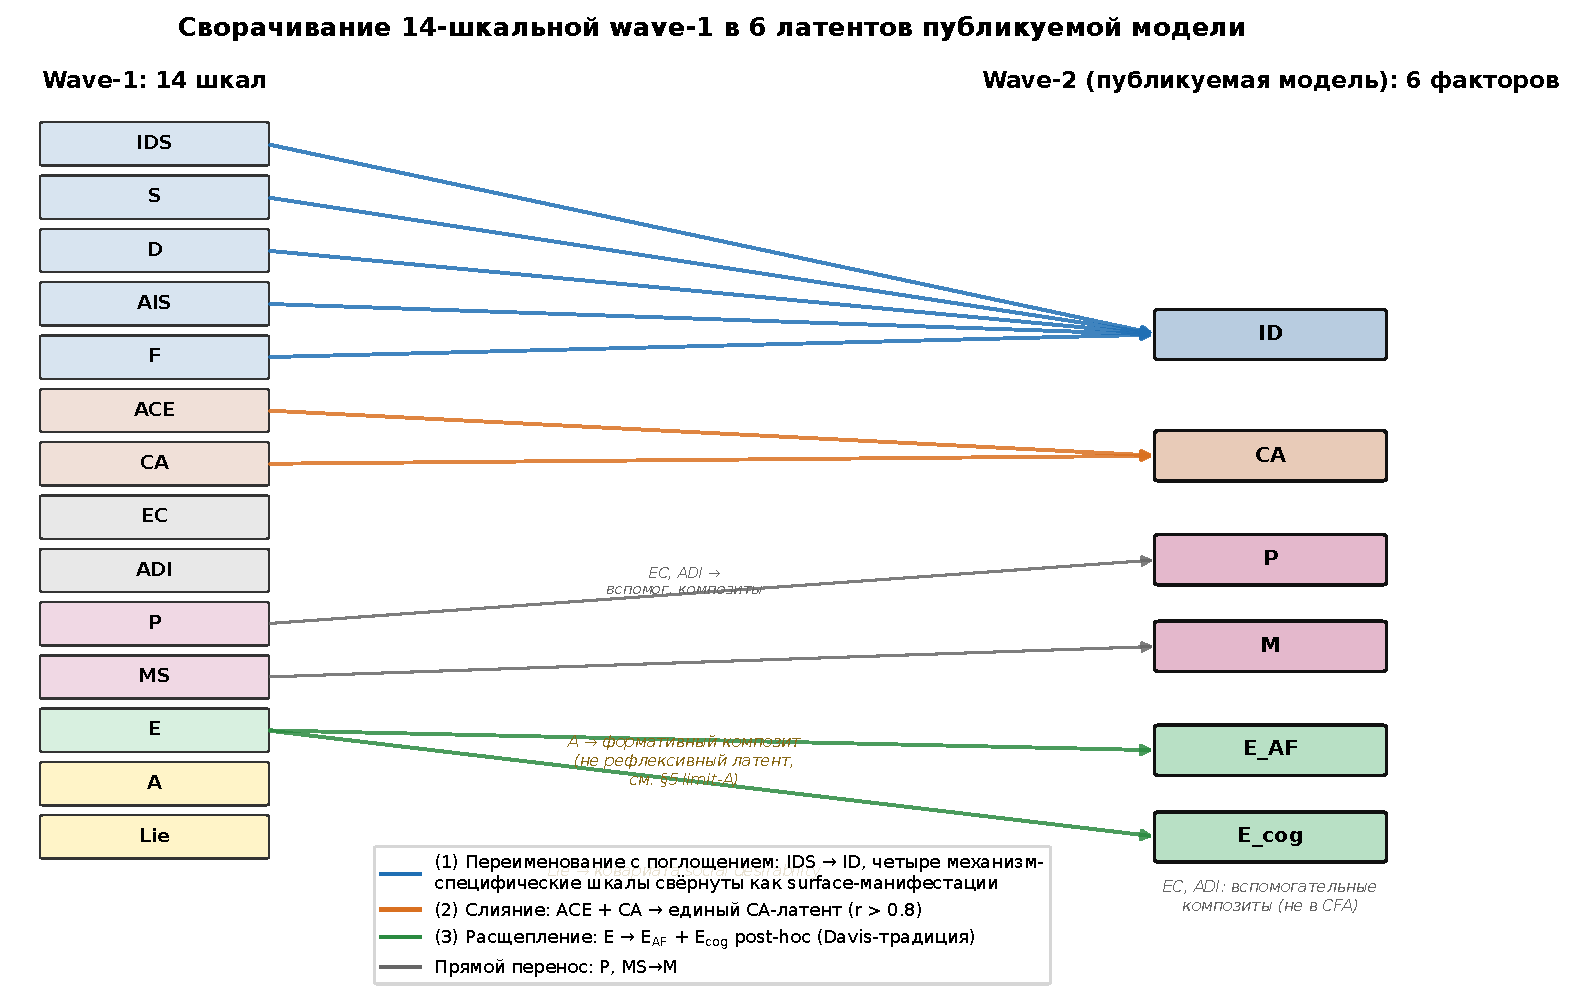
\includegraphics[width=0.95\linewidth]{figures/fig9_wave_mapping.pdf}
\caption[Карта перехода wave-1 $\to$ wave-2]{Карта перехода от 14 wave-1 шкал к 6 латентам публикуемой модели. Синие стрелки --- переименование с поглощением (IDS $\to$ ID, вместе с S, D, AIS, F как surface-манифестации одного поля); оранжевые --- слияние двух индикаторов ранней истории (ACE + CA $\to$ CA); зелёные --- расщепление общей шкалы эмпатии (E $\to$ \EAF{} + \Ecog{}); серые --- passthrough (P, MS $\to$ M). EC, ADI сохранены как вспомогательные наблюдаемые композиты; A, Lie --- контрольные шкалы.}
\label{fig:wave_mapping}
\end{figure}

\emph{Итоговая карта.} 12 содержательных wave-1 шкал $\to$ 6 латентов публикуемой модели: \texttt{IDS} $\to$ \textbf{ID} (переименование с поглощением \{\texttt{S, D, AIS, F}\} как неотделимых surface-манифестаций того же поля); \{\texttt{ACE, CA}\} $\to$ CA (объединение двух индикаторов ранней реляционной истории в единый латент); \texttt{P} $\to$ P; \texttt{MS} $\to$ M; \texttt{E} $\to$ \{\EAF, \Ecog\} (post-hoc расщепление, единственная операция расширения); \{\texttt{EC, ADI}\} $\to$ вспомогательные наблюдаемые композиты. A отделена как формативный композит; Lie --- ковариата social desirability, корректирующая E и ID в прикладных интегральных метриках. Публикуемая шестифакторная структура --- минимальная, которую данные поддерживают. Феноменологические и типологические различия, спрятанные в этой минимальности, --- задача волны 2.

\paragraph{Multi-scale веса в \texttt{questions.json} --- новация и её scoring-артефакт.} Эксплицитное a-priori приписывание каждому айтему вектора весов по нескольким факторам --- существенная содержательная новация инструмента, а не методологическая небрежность: большинство опросников эмпатии делают вид, что simple structure справедлива, и приписывают айтем одной шкале, теряя ту часть дисперсии, которая сидит на пересечениях конструктов. DEIC этот cross-структурный аспект выносит из неявных статистических артефактов в явную теоретическую декларацию, которую можно критиковать и валидировать (ближайший психометрический родственник --- a-priori bifactor-модели). Однако композитное sum-scoring с multi-scale весами алгебраически раздувает корреляции между композитами: пункт с ненулевыми весами в двух композитах засчитывается с обеих сторон уравнения, когда эти композиты коррелируют. В нашей выборке средняя инфляция $\sim 0.18$, максимум $0.68$ с переменой знака P$\leftrightarrow$E. Латентные факторные скоры этой проблемы лишены, потому что CFA корректно разделяет общую и специфичную дисперсию. Wave-2 решение --- не отказ от новации, а её разделение на два независимых слоя в \texttt{questions.json}: \texttt{factor\_weights} (вектор для CFA с явно прописанными cross-loadings --- теоретический слой остаётся) и \texttt{primary\_scale} (единственный фактор для композитного sum-scoring --- один айтем, один композит). Композиты публикуются как ориентировочные без алгебраической инфляции; латентные скоры --- как основной научный результат. Новация сохраняется в полном объёме и становится двухуровневой по конструкции.

\paragraph{Self-report only.} Нет informant-report, нет поведенческих мер, нет физиологических конвергентных измерителей. Особенно критично для A, где self-report имеет circular-validity ограничение (точный отчёт о внимании требует внимания).

\paragraph{Вторичная психопатическая подгруппа мала.} $n = 65$. Rule-based $2 \times 2$ даёт устойчивое направление, но величины эффектов во вторичной ячейке имеют широкие CI и требуют клинической выборки для подтверждения.

\subsection{Дизайн-связанные ограничения}

\paragraph{Cross-sectional.} Нет временной оси, нет pre/post-терапевтического дизайна, нет retest-стабильности. Следствие: невозможно различить стабильный A от транзиторного, невозможно тестировать longitudinal-предсказания, сформулированные в §\ref{subsec:falsifiers}, и невозможно эмпирически различить direction of causation в паре CA--ID (теоретически предполагаемая, но статистически неидентифицированная).

\paragraph{Моноязычная выборка.} Русскоязычный интернет-рекрутинг; выборка self-selected. Культурный, языковой и платформенный bias присутствуют. Cross-cultural валидация (EN, ES, CH, AR) с invariance-testing --- обязательный следующий шаг.

\paragraph{Возрастной перекос} в сторону 18--37; подгруппа 38+ ($n = 50$) мала. Супрессорная медиация устойчива на 18--37, ослабевает 38+; механизм неясен --- post-therapy effects, survivor bias, developmental shift --- и требует возраст-стратифицированной выборки.

\paragraph{Self-selection через Telegram/VK.} Опросник требует intro-метакогнитивного vocabulary; возможно, эта форма селекции уже сдвигает распределение A вправо относительно генеральной популяции. Данные не поддерживают распространение на non-reflexive субпопуляции.

\paragraph{Подвыборка «befriends-psychopaths» и этика индивидуального уровня.}
\label{subsec:limitations_befriends}
Архетип эмпатического контрагента в диаде с психопатом (hi-E $+$ hi-P в октанте $+++-$) эмпирически подтверждён, но представлен в выборке только $n = 3$ респондентами ($0.19\%$). Никто из них не отметил ни одной текстовой диагностической категории, самоописания этого профиля в свободном поле отсутствуют: архетип систематически невидим для self-report. Ретроспективная power-оценка: детектирование $d = 0.5$ в этой подгруппе требует $n \approx 150$, $d = 1.0$ --- $n \approx 30$. В текущей волне профиль зафиксирован описательно, без параметрических сравнений. Wave~2 требует целенаправленного сэмплинга этой конфигурации. \emph{Этическое ограничение:} один из трёх респондентов известен нам биографически, поэтому любые индивидуальные характеристики этой подгруппы публикуются только как агрегированные центроиды ($n = 3$); индивидуальный уровень данных из статьи исключён и не передаётся в открытые supplementary.

\subsection{Статистические ограничения}

\paragraph{Многомерная не-нормальность данных и robust fit indices.} Mardia $p < 0.0001$. Реализованы две приближённые robust-пересчётки. \textbf{(а)}~Bootstrap-аппроксимация Satorra--Bentler scaling (в \texttt{tier4\_analyses.py}). \textbf{(б)}~Satorra--Bentler T$_1$ через \texttt{semopy.stats.calc\_chi2\_sb} с четвёрто-моментной весовой матрицей из \texttt{prepare\_wls} поверх ML-посадки: $\chi^2_{\mathrm{SB}}(120) = 934.25$, CFI$_{\mathrm{SB}} = 0.873$, RMSEA$_{\mathrm{SB}} = 0.098$, scaling factor $c = 0.552$. Нетипичное $c < 1$ (ML-$\chi^2$ дефлирован относительно SB-корректированного) и падение CFI с $0.950$ до $0.873$ --- два независимых сигнала, что содержательные выводы статьи следует оценивать на latent factor scores (устойчивых к этой коррекции), а не на глобальных fit-индексах. Точные MLR SE и WLSMV на сырых ordinal-айтемах требуют \texttt{lavaan} в R для финальной публикации; это инфраструктурный gap, а не содержательный, и reviewer-стандарт его требует эксплицитно.

\paragraph{Conditional process SEM на композитном модераторе A.} После A-CFA корректная реализация --- переход к структурному моделированию A как латента, с учётом его биполярной природы. В текущей форме A-модерация держится на теоретически взвешенном композите; это работает, но требует дублирования в структурной форме.

\paragraph{Post-hoc характер факторного разделения \EAF{}/\Ecog{}.} Разделение когнитивной и аффективной эмпатии было установлено post-hoc в ответ на парадокс P$\leftrightarrow$E в оригинальной модели. Pre-registered replication с айтемами, разведёнными по дизайну, --- необходимое условие для устойчивости этого различения.

\subsection{Теоретические гапы}

Это не ограничения текущей статьи в строгом смысле, а \emph{отсутствующие элементы в теории}, которые программе предстоит заложить. Мы их перечисляем явно, потому что граница известного --- часть эмпирической работы.

\paragraph{Временной каркас.} Теория в текущем виде --- cross-sectional snapshot. Вся содержательная лексика («автоматизм», «осознанность») --- temporal. Требуется трёхшкальный временной фрейм: fast (ms--s, стимул $\to$ активация ID $\to$ подавление \EAF{}), meso (недели--месяцы, repeated A-активации в терапии $\to$ постепенное расцепление), slow (годы--декады, ACE $\to$ формирование ID-паттерна $\to$ рекрутирование P или нет). Планируется отдельная статья «\DEIC{} dynamics: temporal architecture of empathy blocking».

\paragraph{Механизм переключателя ID $\leftrightarrow$ P.} Эмпирически ID и P разделимы. Но \emph{что решает} в конкретном контексте, какой механизм включается --- теория не говорит. Три рамки-кандидата: cost/benefit (P --- когда подавление эмпатии выгодно; ID --- когда чувствование невыносимо), predictive coding (ID --- bottom-up сигнал перегруза; P --- top-down сигнал модели), conflict monitoring (ID блокирует чувство; P блокирует действие). Рабочий выбор --- predictive coding; выход в отдельную статью.

\paragraph{Механизм терапевтической силы A.} A эмпирически модерирует оба пути. Механизм неопределён. Кандидаты: A увеличивает temporal resolution самонаблюдения, ловит защиту до её завершения; A декомпонует automatic binding ID$\leftrightarrow$\EAF{}-suppression; A $=$ метакогнитивная working memory с ограниченной ёмкостью. Выход в отдельную статью.

\paragraph{Individual differences в A-trainability.} Инструмент меряет текущий A, но нет модели того, что \emph{позволяет} A обучаться. Кандидаты: working memory capacity, interoceptive accuracy, language-mediation capacity, safety-context stability. Клиническое значение: предсказание, кто ответит на A-based терапию.

\paragraph{Developmental branching в $2\times 2$.} Первичный/вторичный/травматический/baseline описаны топологически. Каким путём ребёнок оказывается в каждой клетке --- отдельная теоретическая задача. Karpman-гипотеза (первичный конституциональный, вторичный приобретённый) тестируема с ранними CA/temperament-маркерами на lognitudinal детской выборке.

\paragraph{Эволюционно-экологическая подложка.} Почему empathy default-on? Почему два отделимых механизма выключения? Почему P стабилен в популяции как ESS на низкой частоте? \DEIC{} к evolutionary literature не подключён; это ноша для theory-of-everything направления и явно выходит за пределы данной работы.

\paragraph{Рефлексивность наблюдателя.} A наблюдателя --- условие видения A у наблюдаемого. В терапии это операциональная реальность (терапевт с низким A не видит ID-активации пациента). В исследовании --- измерительный аппарат содержит измеряемую величину. Аналогия с observer-problem в квантовой механике --- не мистическая, а структурная. Достойна отдельного методологического раздела в программной статье.

\section{Будущая работа}
\label{sec:future}

Будущая работа \DEIC{} распределена по двум осям: технические расширения (методологические, не требующие теоретической переработки) и фундаментальные продолжения (разработка теоретических гапов из §\ref{sec:limitations}, каждый из которых выводится в отдельную статью программы).

\subsection{Технические расширения}

\paragraph{Pre-registered replication на новой выборке.} Обязательное условие до wide publication. Центральные предсказания --- A-модерация канала CA$\to$ID$\to$\EAF{} в узкой спецификации, коллапс ID-пути в unified SEM при включении P, двухосевое различение первичного и вторичного паттернов, компенсаторная функция A в hi-CA$\times$hi-A группе, положительная partial-корреляция P и \Ecog{} после partialling. Replication должна воспроизвести именно эту комбинацию, включая ре-композицию дисперсии в unified модели.

\paragraph{Item wave 2: инструментальная пересборка.} Приоритетные направления: (1) dedicated A-scale, разведённая по дизайну между witnessing и trauma hypervigilance, с контентной валидизацией на cover всех четырёх лингвистических традиций (satipaṭṭhāna, sākṣī, rigpa, self-remembering); (2) M-редизайн с разведением instrumental и reactive masking; (3) \EAF{}/\Ecog{} разведены на item-level, а не post-hoc; (4) один айтем $=$ один фактор в scoring (без multi-scale весов); (5) P-шкала расширена явной моральной подписью (items о «разрешено мне») отдельно от архитектурных items о resonance switching; (6) ACE-айтемы сохраняют трёхвариантный формат («да» / «нет» / «не помню»), но «не помню» кодируется как эксплицитный \emph{позитивный} сигнал (семейное замалчивание или диссоциативный encoding-gap), а не missing; счётчик таких ответов по всем 10 айтемам формирует pre-registered ACE-dissociation подшкалу с заявленными критериями McDonald's $\omega \ge 0.7$ и $r(\text{ACE-dis}, \text{ID}_{\mathrm{lat}}) \ge 0.30$. Post-hoc re-fit на wave-1 (§\ref{subsec:ace_extension}) показывает усиление латентной связи $r(\text{CA}, \EAF{})$ с $-0.129$ до $-0.205$ и появление статистически отличимого от нуля индиректа через P --- wave-2 должна pre-register эту логику и подтвердить её как установленный факт.

\paragraph{Лонгитюдное расширение} (6--12--24 месяца, in-therapy subgroup). Тестирует стабильность A, траекторию integration, test-retest-надёжность всех шести факторов. Выборка с явной стратификацией по therapy-status (in-treatment, post-treatment, never-treated) позволит различить стабильное и транзиторное A.

\paragraph{Мультикультурная валидация} (EN, ES, CH, AR) с invariance-testing (configural $\to$ metric $\to$ scalar). Проверка обобщаемости архитектуры за пределами русскоязычной выборки.

\paragraph{fMRI-конвергенция.} DMN $\times$ attention-networks co-activation как нейро-коррелат A. Биологическая грануляция A-конструкта через существующие neuroimaging-парадигмы (resting-state functional connectivity, mindfulness-induced DMN-deactivation).

\paragraph{Informant report на субвыборке.} Круговая валидность особенно важна для A и P, где self-report имеет структурные ограничения.

\paragraph{Behavioral convergents для A.} Dual-task paradigms, interoception accuracy tasks (heartbeat detection), mind-wandering probes --- выход из чистого self-report.

\subsection{Фундаментальные продолжения}

Это статьи программы, разрабатывающие теоретические гапы §\ref{sec:limitations}.

\paragraph{«\DEIC{} dynamics: temporal architecture of empathy blocking».} Трёхшкальный временной фрейм (fast/meso/slow), связь с active inference и predictive coding. Эмпирические корреляты через micro-longitudinal (daily diary) и neurocognitive (ERPs) парадигмы.

\paragraph{«ID and P as directional asymmetries of empathic prediction».} Разделение bottom-up ID и top-down P в рамке predictive coding. Interoceptive accuracy tasks как дифференциатор: ID-пациенты должны иметь дефицит интероцептивной точности; P-пациенты --- сохранную интероцепцию при сниженной моральной salience чужого дистресса.

\paragraph{«What does attention do: candidate mechanisms for the A-moderator effect».} Трёхканальная теоретическая работа: temporal resolution, automatic binding decomposition, metacognitive working memory. Empirical probes через phasic attention tasks и dual-task paradigms.

\paragraph{«Individual differences in A-trainability: who benefits from witnessing-based therapy?»} Pre-treatment predictors эффекта A-based interventions. Кандидаты: working memory capacity, interoceptive accuracy, language-mediation, safety-context stability. Клиническая выборка с RCT arm.

\paragraph{«Developmental branching in $2\times 2$ psychopathic topology».} Longitudinal child sample с early CA/temperament-маркерами; тест Karpman-гипотезы о двух путях в первичную vs вторичную клетку.

\paragraph{«\DEIC{} and the reflexivity of measurement: observer-A as part of the instrument».} Методологическая статья о том, что A наблюдателя --- условие возможности видеть A у наблюдаемого. Эпистемологически: структурная, не мистическая аналогия с observer-problem в квантовой механике. Операциональные следствия: supervision-требования для клиницистов, A-assessment исследователя как часть методологического репортинга.

\paragraph{«Free will as a gradient of attention: an operational reading».} Отдельная философско-психологическая статья, развивающая §\ref{subsec:free_will}. Предлагает переформулировку проблемы свободы воли как проблемы измеримой A-инфраструктуры, с проверяемыми предсказаниями: корреляция ощущения свободного выбора с моментальным A (а не trait-self-efficacy), прирост self-determination-маркеров после A-интервенций, структурная функциональная несвобода в low-A-популяциях. Разворачивает этические следствия (перекалибровка ответственности, прощение как эпистемологическая корректность), без отмены различения между low-A-автоматизмом и A-поддержанным P-выбором.

\paragraph{«Pharmacology as DEIC-modification: a stratification-based prediction map».} Статья, формализующая таблицу «класс веществ --- модификация компонента D/P/A --- предсказание по профилю --- proposed clinical test», развёрнутую в §\ref{subsec:pharmacology_nosology}. Ядро --- дифференциальные предсказания: psilocybin большой эффект на D-dominant, малый/обратный на P-dominant; MDMA уникален как E-ceiling$+$D-dissolve$+$A-preserve; ketamine как «диссоциация для растворения диссоциации» с responders$=$hi-D baseline; opioid dependence как safety-deficit-D-signature. Предлагаемая эмпирическая программа: retrospective re-analysis существующих psilocybin/MDMA RCT с DEIC-profile на baseline как модератором ответа.

\paragraph{«The structural under-sizing of modern mental healthcare: what early-formation D requires».} Клинико-институциональная статья, развёртывающая §\ref{subsec:undersizing}. Ядро: argument for a structurally different scale of intervention for personality-formative early D, с обзором методов адекватного масштаба (длительный интенсивный психоанализ, psychedelic-assisted protocols с extended integration, therapeutic communities, multi-year somatic work) и картой «что сейчас недоступно». Не манифест; эмпирическая программа по proof-of-concept: DEIC-стратификация на baseline как предиктор ответа на symptom-level vs structural-level интервенции.

\paragraph{«DEIC и populational-level predictions: attention economy, politics, collective D».} Статья, разворачивающая §\ref{subsec:political}. Предсказания: (а) интенсивность использования engagement-оптимизированных платформ снижает A в 6--12-месячных лонгитюдах; (б) подростковые когорты с ранним algorithm-exposure имеют измеримо иную DEIC-топологию при том же ACE-load; (в) электоральная поддержка P-стилевой демагогии предсказывается general A-уровнем аудитории; (г) DEIC-профили ex-cult и ex-radicalised лиц характеризуются low A с сохранённым подавленным D. Данные для (а)--(г) требуют cross-cohort и cross-cultural дизайнов.

\paragraph{«Evolutionary mismatch and the biological necessity of integration».} Программная статья, развивающая §\ref{subsec:evolutionary}. Тезис: современный взрослый человек --- первый в истории вида, для которого интеграция есть биологическое требование, а не культурная роскошь. Эмпирическая программа: population-level траектории A-индикаторов (distress tolerance, boredom capacity, sustained attention) в связи с urban engagement-density; инцидентность D-dominant расстройств в зависимости от разрыва между ACE-load и доступностью integration-инфраструктуры; 20--40-летние когортные сравнения когорт с и без структурного доступа к integration-систем.

\paragraph{«Nosological reorganization: DEIC-profile as a trans-diagnostic stratifier».} Эмпирическая статья, проверяющая способность DEIC-профиля на baseline захватывать больший процент дисперсии клинического ответа и траектории, чем DSM-метка, в large-scale retrospective re-analysis. Совместимость и параллель с HiTOP и RDoC; falsification: если DEIC-профиль не даёт прироста над diagnosis label --- рамка ограничивается более узкими применениями, нозологическая претензия снимается.

\subsection{Прикладные направления}

\paragraph{Клинические RCT.} Head-to-head тесты: non-dual mindfulness vs MBSR в работе с ID-доминантными клиентами; A-training arm vs 12-step в substance-use с блокирующим профилем; sequenced A-work $\to$ CBT vs CBT-first в treatment-resistant депрессии.

\paragraph{DEIC как решение проблемы под-диагностирования (collaborative-filtering подход).} Прямое расширение §\ref{subsec:dx_count_bias}. Наблюдение, что инструмент систематически ловит именно тех, кого self-report диагностика пропускает (hi-P --- через ROC AUC $< 0.5$ на mood/anxiety/neurodev; hi-ID --- через help-seeking block; ранне-травматический hi-CA --- через «не знаю» как дис­со­циа­тив­ный сигнал), переворачивается в позитивный дизайн. Классическая нозология предсказывает диагноз от сообщённых симптомов; DEIC-coordinates устойчивы в архитектурно-похожих группах, поэтому k-NN / latent-class similarity на 6-факторном профиле позволяет предсказывать \emph{вероятностный клинический ландшафт} для нового респондента по близости к подвыборке с известными диагнозами --- стандартная формулировка collaborative filtering, но с клинической целевой переменной. Дизайн проверки: wave с recruitment через первичку и образовательные институции (вне мем-канала, чтобы разорвать selection bias), DEIC на входе, структурированное клиническое интервью (SCID/MINI) в слепую относительно DEIC-профиля как gold standard; метрики --- sensitivity/specificity DEIC-скрининга к клиническим меткам, incremental AUC над симптомным скринингом (PHQ, GAD), калибрационные кривые для «архитектурно обусловленного» прогноза. Публичный смысл тоньше, чем звучит: цель --- не автоматическая маркировка людей, а снятие bottleneck на распознавание там, где сам механизм патологии блокирует распознавание. Ограничения очевидны (риск false-positive разметки, этика скрининга без согласия, необходимость human-in-the-loop клинициста) и должны быть предметом отдельной прикладной рамки.

\paragraph{Публичная коммуникация.} Отдельная рамка «травма не приговор» разработана вне академического слоя и требует собственной эмпирической валидизации на non-academic аудитории. Тезисы: integrated-survivor как эмпирически-обоснованный горизонт восстановления; различение wellness-industry toxicity от contemplative substance; A-work как путь, а не обещание счастья.

\paragraph{Политическая и организационная коммуникация.} P-style демагогия и low-A аудитории --- testable hypothesis с cross-sectional audience studies. Организационная психология: применимость условной-архитектурной рамки в подборе и supervision ролей, требующих эмоциональной регуляции (медицина, helping professions, силовые структуры).

\paragraph{Образование.} A-oriented школьные программы как primary prevention для CA-высоких когорт. Связь с existing SEL (social-emotional learning) инициативами; эмпирическая проверка, работают ли SEL-программы на механизм, который \DEIC{} постулирует.

\paragraph{Attention-protective институциональная инфраструктура.} Прикладное продолжение §\ref{subsec:political}. Дизайн и оценка interventions уровня дизайна медиа-продуктов (slow-feed, pause-интерфейсы, edit-mode), уровня школьных программ (contemplative education как компонент общего curriculum), уровня регуляции (engagement-оптимизация как public health issue). Testable: дают ли такие изменения измеримый прирост A в популяции при прочих равных.

\paragraph{Свидетельская работа коллективной D: transitional justice как DEIC-операция.} Прикладная статья о том, как DEIC-координаты могут давать количественную меру тому, что transitional justice и memorial practices делают интуитивно: коллективная D-work через создание публичного пространства для аффективной интеграции исторической реальности. Пилотные данные --- на post-tоталитарных обществах с доступными longitudinal social-psychological данными.

\subsection{Мета-программа}

\paragraph{Методологическая статья программы.} Формальное изложение дисциплинарных правил анти-Уилбер (§\ref{subsec:discipline}), reflexivity clause, observer-A problem. Место: статья \#18 в программе, выходит после эмпирического ядра.

\paragraph{Открытая документация программы.} \texttt{PROGRAM\_STRUCTURE.md} в репозитории содержит полный список 18 планируемых статей с их falsifiers и expected deliverables. Каждая замыкается либо pre-registered replication, либо явным обновлением программы при non-replication. Это и есть форма, в которой мы принимаем обязательства --- распределённая во времени сеть проверяемых утверждений, а не завершённая теория.

Текущая статья --- узкая по тону, скромная в претензиях --- защищает возможность развернуть амбициозную программу. \DEIC{} как каркас стоит на том, что каждая из его будущих работ может быть опровергнута в своей точке, и если значительная их часть опровергнется, каркас как целое подлежит пересмотру. Иначе мы работаем не в психометрии, а в риторике.


\bibliographystyle{plainnat}
\bibliography{refs}

% ======================================================================
% Supplementary materials — methodological checks not central to the core claims
% Extracted from §Results 2026-04-20 to keep the main narrative focused.
% All ref labels from main text remain valid (\ref{subsec:limitations_befriends},
% \ref{subsec:conditional_process}, \ref{subsec:unified_sem}).
% ======================================================================

\appendix
\section*{Приложение S1. Дополнительные методологические проверки}
\label{supp:round3}

Содержание приложения: LPA/GMM на четырёх композитах, статус ADI как самостоятельной оси, DI vs Lie-scale, октантная карта категорий свободного поля, piecewise-линейная траектория «burning empath», network-centrality после GLasso. Каждое наблюдение поддерживает или уточняет один из основных findings §Results, но не несёт самостоятельной claim-нагрузки уровня headline-результатов.

\subsection*{S1.1 LPA / GMM на четырёх композитах}
Latent profile analysis на E, P, D, A под BIC выбирает $k=2$. Кластер 0 ($n = 1461$, «нормальный»): $E = 55.8$, $P = 42.5$, $D = 52.2$, $A = 55.1$. Кластер 1 ($n = 90$, $5.8\%$ выборки): $E = 40.2$, $P = 65.2$, $D = 55.9$, $A = 42.9$ --- именно P-полюс. Из 90 человек кластера~1, 54 попадают в квадрант «low E / high P» в 2D-проекции. То есть даже чистая mixture-модель на четырёх шкалах, без априорных меток, выделяет психопатический контур как самостоятельный естественный класс. Расширение до $k=3, 4, 5$ под BIC не даёт улучшения, на которое можно было бы опираться: $k=3$ даёт $\Delta\mathrm{BIC} = -32$, но третий кластер --- это крошечная $n = 14$ «dissociated low-A» подгруппа, структурно не новая относительно high-D подвыборки.

\subsection*{S1.2 ADI не самостоятельная ось}
Anti-Dissociation Index (ADI), рассматриваемый в части психометрической литературы как самостоятельный конструкт, в наших данных практически совпадает с $D_{\mathrm{score}}$: $r(\mathrm{ADI}, D) = +0.806$, $r(\mathrm{ADI}, \mathrm{AIS}) = +0.770$, $r(\mathrm{ADI}, \mathrm{IDS}) = +0.786$, $r(\mathrm{ADI}, P) = +0.065$ (практически ноль). ADI --- это свёртка блокировочного пояса, не отдельная латентная координата. Мы поэтому не включаем ADI как независимый предиктор в основные модели; в описательной статистике он работает как global severity index для защитного полюса, не более.

\subsection*{S1.3 DI не сводится к социальной желательности}
Discrepancy Index (разрыв между self-reported E и поведенческими маркерами) в часто задаваемом вопросе «не Lie ли это?» получает отрицательный ответ: контраст HIGH-DI vs LOW-DI подгрупп по Lie-шкале даёт $d = 0.00$ ($p = 0.99$). В совместной модели $\mathrm{DI} \sim A + P + D + \mathrm{Lie} + \mathrm{ACE}$ ($R^2 = 0.41$) Lie вносит минимальный вклад; основные драйверы --- $A$ ($+$), $P$ ($-$), $D$ ($+$). DI --- реальный структурный паттерн «аффективная эмпатия, которая не становится действенной», а не артефакт стиля ответа.

\subsection*{S1.4 Октантная карта 8/16}
Проекция категорий свободного поля на октанты (знаки $z$-оценок E, P, D, A) заполняет лишь 8 из 16 возможных октантов; 8 октантов остаются пустыми. Интересны два пустых: $++++$ (все четыре шкалы одновременно высокие) --- структурно ожидаемо пуст, так как hi-E и hi-P дают противоположные требования к архитектуре; и $+++-$ (hi-E, hi-P, hi-D, low-A) --- архетип «дружит с психопатом / эмпатический контрагент», на него приходится только $n = 3$ респондента (см. §\ref{subsec:limitations_befriends}). Остальные шесть пустых октантов --- теоретически возможные, но не представленные в выборке конфигурации; их заполнение требует таргетированного подбора подвыборок в wave~2.

\subsection*{S1.5 «Burning empath» как piecewise-линейная траектория}
Нелинейный piecewise-регрессионный анализ $\mathrm{ACE} \to E_{\mathrm{AF}}$ с оптимальным knot~$= 80$ (из 100-балльной шкалы ACE) показывает два режима: до 80 $\beta = -0.085$ ($p < 10^{-7}$), после 80 $\beta = -0.498$ ($p = 7 \times 10^{-4}$). $\Delta\mathrm{AIC} = -5.37$ против чисто линейной модели --- улучшение существует, но скромное. На бинах среднее \EAF{} монотонно падает с $57.97$ (ACE $[0, 30]$) до $51.70$ (ACE $[75, 100]$). Содержательный вывод: «сгорающий эмпат» как качественно отдельная траектория в данных \emph{не выделяется}; основной эффект CA на \EAF{} линейный, нелинейный догиб в экстремальном хвосте ACE присутствует, но не меняет общую картину.

\subsection*{S1.6 Network centrality: ACE и F --- центральные хабы}
Partial-correlation network на $\{$E, P, D, A, ACE, F, EC$\}$ после GLasso-регуляризации даёт strength centrality (сумма $|$partial $r|$): $\mathrm{ACE} = 3.43$, $F = 3.42$, $D = 3.11$, $\mathrm{EC} = 2.95$, $P = 2.60$. То есть ранний адверсивный анамнез (ACE) и компонент «F» внутри $D$-пояса (аффективная дизрегуляция) --- самые сильно связанные узлы сети. Мост между $D$-кластером и ACE проходит через $F$. Сетевая структура подтверждает каузальное предположение статьи «ACE $\to$ F $\to$ D-каскад $\to$ \EAF{}» на уровне условных зависимостей.

\subsection*{S1.7 Эмпирическая производная архетипной архитектуры}
\label{supp:empirical_archetypes}

В продуктовом слое инструмента (\texttt{cluster} field в экспортируемых данных) каждому респонденту присваивается архетипный ярлык из 12 категорий (Трикстер, Странник, Аналитик и др.). Эта декомпозиция rule-based и по конструкции декоративная; её эмпирическая воспроизводимость не была проверена в основной статье. Здесь мы тестируем вопрос напрямую: \emph{какая кластерная структура естественно поддерживается данными в 6-факторном пространстве}.

\paragraph{Метод.} На стандартизованных 6-факторных композитах (E, P, M, A, ID, CA; $N = 1465$) выполнены $k$-means кластеризации при $k = 2$--$10$. Для каждого $k$ вычислены: silhouette index, общий within-sum-of-squares, и bootstrap-стабильность через Adjusted Rand Index ($50$ итераций случайных 50\%-подвыборок).

\paragraph{Стабильность.} ARI как функция $k$:

\begin{center}
\begin{tabular}{ccc}
\toprule
$k$ & ARI mean & интерпретация \\
\midrule
2 & 0.91 & очень стабильно (P-pole vs healthy) \\
3 & 0.81 & стабильно \\
\textbf{4} & \textbf{0.72} & \textbf{стабильно (рекомендуемое разрешение)} \\
5 & 0.62 & стабильно \\
6 & 0.48 & пограничная стабильность \\
8 & 0.46 & пограничная \\
10 & 0.45 & пограничная \\
\bottomrule
\end{tabular}
\end{center}

Структура $k = 4$ выбрана как оптимальный баланс между стабильностью (ARI~$> 0.70$) и интерпретативной разрешающей способностью.

\paragraph{Четыре эмпирически устойчивых кластера.}

\begin{center}
\small
\begin{tabular}{lrrrrrrr}
\toprule
Кластер & $n$ ($\%$) & $E$ & $P$ & $M$ & $A$ & ID & CA \\
\midrule
\textbf{Свидетель} & 358 (24\%) & $+0.88$ & $-0.71$ & $-0.98$ & $+0.88$ & $-1.15$ & $-0.60$ \\
\textbf{Защищённый} & 313 (21\%) & $-1.19$ & $+1.03$ & $+1.07$ & $-0.98$ & $+1.05$ & $+0.53$ \\
\textbf{Раненый} & 453 (31\%) & $+0.09$ & $-0.52$ & $-0.11$ & $-0.41$ & $+0.35$ & $+0.65$ \\
\textbf{Оператор} & 341 (23\%) & $+0.04$ & $+0.49$ & $+0.19$ & $+0.53$ & $-0.22$ & $-0.73$ \\
\bottomrule
\end{tabular}
\end{center}

Все четыре центроида читаются как теоретически осмысленные DEIC-конфигурации: \emph{Свидетель} объединяет baseline-empath и часть integrated-survivor (§\ref{subsec:integrated}); \emph{Защищённый} соответствует secondary-psychopathy архитектуре (§\ref{subsec:primary_secondary}) с активным P-нарративом, защитной маскировкой и hi-CA + hi-ID; \emph{Раненый} --- канонический trauma-marked профиль без P-надстройки; \emph{Оператор} --- функциональный non-traumatized с конституциональным P-narrative и сохранным witnessing.

\paragraph{Сравнение с продуктовым 12-архетипным слоем.} Для каждого из 12 продуктовых архетипов вычислена доля респондентов, попадающих в доминирующий empirical cluster (k = 4). Ни один из 12 не достигает критерия consistency $\geq 70$\%:

\begin{center}
\small
\begin{tabular}{lrr}
\toprule
Продуктовый архетип & $n$ & Доля в доминирующем emp-cluster \\
\midrule
Воин & 18 & 50.0\% (мал $n$) \\
Аналитик & 289 & 33.2\% \\
Странник & 362 & 35.0\% \\
Трикстер & 377 & 28.9\% \\
Шаман & 37 & 48.6\% \\
\textit{(все остальные)} & --- & $< 50\%$ \\
\bottomrule
\end{tabular}
\end{center}

Каждый продуктовый архетип распределён по всем четырём empirical-кластерам приблизительно равномерно. Архетипное именование в текущем виде \emph{не воспроизводит} наблюдаемой структуры данных и должно интерпретироваться как декоративный narrative shorthand для product-feedback, не как эмпирически валидная типология.

\paragraph{Импликация для wave-2 и для public framing.} Для replication-ready кластерной системы инструмент должен переключиться с rule-based 12-архетипа на data-driven 4-cluster (Свидетель / Защищённый / Раненый / Оператор) с явной коммуникацией респонденту: \emph{кластер --- статистически воспроизводимый регион непрерывного 6-факторного пространства, не categorical тип личности; респондент со временем может смещаться между кластерами по мере изменения архитектуры}. Эта переформулировка снимает критику D\&D-class-style identity-typing, которой подверженно текущее labelling. Empirical cluster definitions, criteria, центроиды и caveats формализованы в \texttt{psychometrics.json:empirical\_clusters} (см.\ \texttt{empirical\_archetypes\_summary.json} в supplementary materials).


\end{document}
